\documentclass[table]{dissertation}
\geometry{twoside=false}

\usepackage{syntonly}
%\syntaxonly

%\usepackage[none]{hyphenat}
%\sloppy

\usepackage{enumitem}
\renewcommand\labelitemi{---}

\usepackage{moreenum}

% Table configuration
\setlength{\tabcolsep}{14pt}
\renewcommand{\arraystretch}{1.5} 
\renewcommand\tabularxcolumn[1]{m{#1}}
%\setlength\arrayrulewidth{1pt}\arrayrulecolor{white}
%\rowcolors{2}{tudelft-dark-blue!20}{tudelft-dark-blue!10!anthracite!20}

% bibliography configuration
\usepackage{csquotes}
\usepackage[style=apa, natbib, backend=biber, bibencoding=utf8]{biblatex}
\DeclareLanguageMapping{american}{american-apa}
\usepackage[strings]{underscore}

\DeclareFieldFormat{doi}{%
%    \mkbibacro{DOI}\addcolon\space
    \mkbibacro{}
    \ifhyperref
    {\href{https://doi.org/#1}{\nolinkurl{https://doi.org/#1}}}
    {\nolinkurl{https://doi.org/#1}}}

%\usepackage[style=apa, natbib, backend=biber, bibencoding=utf8]{biblatex}
%\DeclareLanguageMapping{american}{american-apa}
\addbibresource{references/References.bib}

\usepackage[all]{nowidow}

\usepackage[capitalize, nameinlink]{cleveref}

\graphicspath{ {./images/} }

\begin{document}

%% Specify the title and author of the thesis. This information will be used on
%% the title page (in title/title.tex) and in the metadata of the final PDF.
\title[A Comparative Analysis]{Robust Decision Support Methods}
\author{Erin}{Bartholomew}

%% Use Roman numerals for the page numbers of the title pages and table of
%% contents.
\frontmatter

\newcommand\textcaps[1]{\textsc{\MakeUppercase{#1}}}

\begin{titlepage}

%%\begin{center}
%
%\makeatletter
%{\largetitlestyle\fontsize{18}{18}\selectfont\MakeUppercase{\@firstname{} \@lastname}}
%\makeatother
%
%%% Extra whitespace at the top.
%%\vspace*{2\bigskipamount}
%\vspace*{\fill}
%
%%% Print the title.
%{\makeatletter
%    \largetitlestyle\Huge\selectfont\MakeUppercase{\@title}
%%    \largetitlestyle\color{tudelft-cyan}\Huge\@title
%    \makeatother}
%
%%% Print the optional subtitle.
%{\makeatletter
%\ifx\@subtitle\undefined\else
%    \bigskip
%    \largetitlefont\titleshape\fontsize{18}{18}\MakeUppercase{\textbf{\@subtitle}}
%\fi
%\makeatother}
%
%%\end{center}
%
%\vfill
%
%\makeatletter
%{\largetitlestyle\fontsize{12}{12}\selectfont \MakeUppercase{Delft University of Technology}}
%\makeatother

\cleardoublepage
\if@twoside\else
    \thispagestyle{empty}%
    \vspace*{\fill}%
    \newpage%
\fi
\thispagestyle{empty}

\begin{center}

%% The following lines repeat the previous page exactly.

\vspace*{2\bigskipamount}

%% Print the title.
{\makeatletter
    \largetitlestyle\fontsize{24}{24}\selectfont\MakeUppercase{\@title}
%    \largetitlestyle\color{tudelft-cyan}\Huge\@title
    \makeatother}

%% Print the optional subtitle.
{\makeatletter
\ifx\@subtitle\undefined\else
    \bigskip
    \largetitlefont\titleshape\fontsize{18}{18}\MakeUppercase{\textbf{\@subtitle}}
\fi
\makeatother}

\bigskip
\bigskip
{\Large Master thesis submitted to Delft University of Technology

in partial fulfillment of the requirements for the degree of

\bigskip

\textbf{\LARGE Master of Science}

\bigskip

in Engineering and Policy Analysis 

Faculty of Technology, Policy and Management}

{\large by}
%door

\bigskip
\bigskip

%% Print the full name of the author.
\makeatletter
{\LARGE \@firstname{} \@lastname}
\makeatother

\bigskip
\bigskip

{\Large To be defended in public on August 28 2018}

\vfill

\end{center}

%\clearpage
\thispagestyle{empty}

%% List the committee members
\medskip\noindent
\begin{tabularx}{\linewidth}{lll}
    Student number:     &   4627237                                                 & \\
    Project duration:   &   9 February 2018 -- 29 August 2018                       & \\
    Thesis committee:   &   Prof.\ dr.\ A.\ Verbraeck,                              & TU Delft, Chair \\
                        &   Dr.\ J.\ Kwakkel,                                       & TU Delft, first supervisor \\
                        &   Dr.\ M.\ Warnier,                                       & TU Delft, second supervisor \\
\end{tabularx}

\vspace{4\bigskipamount}

\medskip
\noindent An electronic version of this thesis is available at \url{http://repository.tudelft.nl/}.

\end{titlepage}


\chapter{Preface}

This study presents the results of 6 months of research completed at TU Delft in partial fulfillment of a masters degree in Engineering and Policy Analysis. It is intended to be read by people with a basic background in exploratory modeling and policy analysis. This study seeks to provide an in depth comparative framework that guides the comparison of multiple methods of decision support, The framework is as applied to a series of three methods under conditions of three variations of a single problem to develop a stronger understanding of how each of the three methods responds to different forms of deeply uncertain problems. 

Anyone seeking insight into the trade-offs that exist between the methods of decision support considered in this study, or who are interested in comparing other methods of decision support is welcome to read this thesis. Included is a thorough background of exploratory modeling, robust decision making a detailed comparative framework, including a development package to replicate these results and run new comparisons, an innovative approach to multi-objective optimization, and a discussion of the trade-offs existing between the selection of methods used in this study.

An early version of this study was presented at the	9th International Congress on Environmental Modelling and Software in June 2018 with a presentation called "On the role of scenarios in designing robust strategies: a comparison of MORDM, multi-scenario MORDM and Robust Optimization".

\vspace{25pt}

This thesis would not have been completed without my friends and family, who provided advice, unending support, and an escape when work stalled and I desperately needed some perspective. 

I would also like to thank my graduation committee (chaired by Prof. Dr. Alexander Verbraeck and with second supervisor Dr. Martijn Warnier) and especially my first supervisor, Dr. Jan Kwakkel for their support and advice throughout the completion of this thesis. The idea for this thesis was first introduced to me by Dr. Kwakkel as an opportunity to explore a wide range of methodologies used in the growing field of decision making for problems with deep uncertainty. Through research into this topic, along with conversations with Dr. Kwakkel, the members of my committee, and other members of the faculty of Technology, Policy, and Management, I was able to gain a deeper understanding of both the power and limitations of decision making involving complex and wicked problems. 

I hope this study is helpful to all who read it, and good luck!

Erin Bartholomew 

28 August 2018

%\chapter{Acknowledgments}


Delft, 29 August 2018

\chapter{Summary}
Wicked problems like those identified as Millennium Development Goals by the United Nations require an innovative approach for analysis and solution development \citep{UnitedNations2015}. The characteristics of wicked problems, including no definitive problem formulation, no one solution to the problem, conflicting objectives, and no right to be wrong \citep{Rittel1973}. These problems, therefore, are characterized by a level of uncertainty greater that that which can be addressed with simple probabilities or statistics known as deep uncertainty. And these deeply uncertain problems demand new methods of analysis that go beyond a traditional predict-then-act format which seeks a single optimal solution. Instead of seeking the optimal solution, these new methods focus on finding a set of robust solutions that balance conflicting objectives and perform well under a variety of possible futures. 

Several methods have been developed that aim to do just that, identified in this thesis as robust decision support methods, several methods of which were developed following the structure of robust decision making, introduced by \citep{Lempert2002}. Each method developed takes its own approach to determining a set of robust policy alternatives to decision makers. The choice of which method to use, therefore, will have a significant impact on the results of analysis for both decision makers and policy analysts.  Though there has been some work to compare the efficacy of these methods, no structured comparative framework has been developed that supports the fair comparison of multiple methods of robust decision support. Furthermore, despite the fact that method performance is likely largely dependent on the problem and policy implementation structure, existing comparative literature has consistently made use of a single problem and policy structure. 

\vspace{\baselineskip}
{\Large {\color{title}Goal of Research}}
\vspace{0.5\baselineskip} \newline
To that end, the following research question will be addressed: 

\begin{researchquestion}{Research Question}
    What are the trade-offs between different methods of decision support when considering a wicked problems and varying policy implementation structures? 
\end{researchquestion}

This thesis is proposing a well structured comparative framework that supports a fair comparison of robust decision support methods when considering a wicked problem with multiple types of policy implementation structures. Comparison metrics include those related to the setup of the required models and method implementations, how and when each method communicates results of an analysis, and comparison of the results themselves (including robustness of recommended policies and computational cost of execution). 

\vspace{\baselineskip}
{\Large {\color{title}Methods Considered}} 
\vspace{0.5\baselineskip} \newline
This framework is then utilized to compare the efficacy of three robust decision support methods: MORDM, multi-scenario MORDM, and MORO. To support comparison of these methods, a common structure was established that is strongly rooted in the robust decision making structure \citep{Lempert2006}. This structure, visualized in \cref{fig:diff-flows-summary}, highlights the variation between the three methods, which lies in the policy alternative determination step. 

\begin{figure}[ht]
    \centering
    \captionsetup{justification=centering}
    
    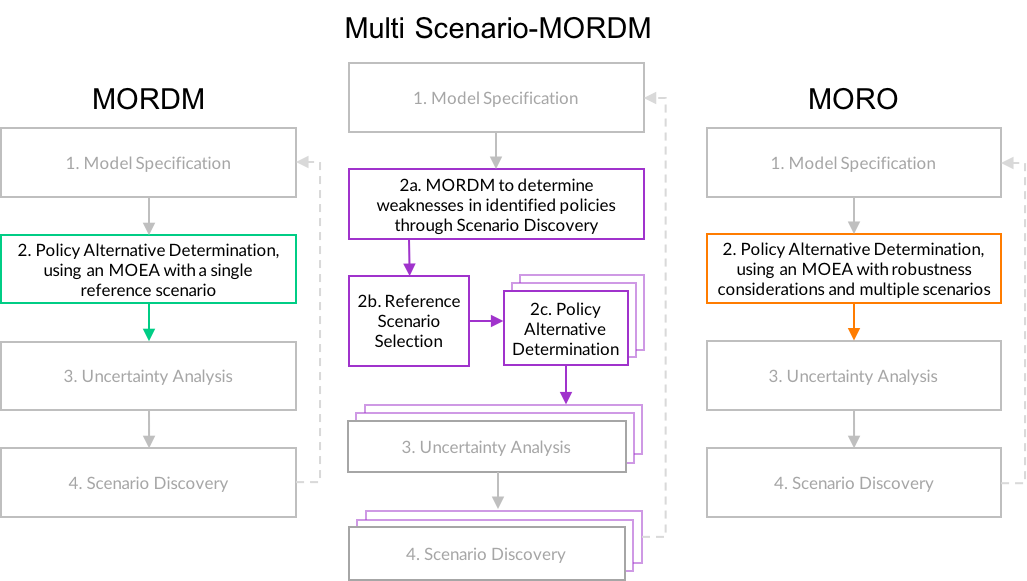
\includegraphics[width=\textwidth]{diff-flows}
    \caption{Comparison of robust decision support framework structures}
    \label{fig:diff-flows-summary}
\end{figure}

The policy alternative determination step in each of the three methods uses a common multi-objective evolutionary algorithm (MOEA) to build a library of potentially robust policy alternatives that will be studied further in the remaining steps of analysis. This thesis uses an algorithm called auto-adaptive $\epsilon$-NSGAII, an innovative MOEA that combines the best features of traditional $\epsilon$-NSGAII, a generational structure and epsilon dominance, with the strongest elements of Borg: auto-adaptive operator selection and adaptive population sizing.

Auto-adaptive $\epsilon$-NSGAII uses evolutionary search techniques to find potentially robust combinations of decision lever values. The fitness of these potential policies is compared using a comparison mechanism, with the alternatives that are not Pareto dominated being added to a set of policies which approximates the Pareto front of the decision lever space. This comparison mechanism is the element of each method that makes it unique. The other elements of each method, including model specification, MOEA parameterization, uncertainty analysis, and scenario discovery, are common to all three methods. 

MORDM uses a single reference scenario to compare the performance of potential policy alternatives, which is generally established with input from decision makers. Multi-scenario MORDM uses a set of reference scenarios that were selected from the vulnerable uncertainty space identified by scenario discovery in a traditional MORDM analysis. The search for alternatives is then run independently for each selected reference scenario. In this way, multi-scenario MORDM attempts to incorporate robustness into the search process. And finally, MORO directly considers robustness of potential policy alternatives by comparing the fitness of policies based on their robustness, calculated with the performance of a policy against a small ensemble of scenarios. 

\vspace{\baselineskip}
{\Large {\color{title}Problem and Policy Structures Considered}}
\vspace{0.5\baselineskip} \newline
The efficacy of each method was tested using a commonly referenced and highly stylized environmental planning problem called the shallow lake problem. 

Three variations of the lake problem are used, which provides the opportunity to compare the efficacy of each method given a wide range of policy structures. The first, labeled intertemporal, represents a static structure, where a predetermined set of decision levers equal to the number of time steps considered (100 in this study) that specifies the anthropogenic pollution released in each time step. The second, direct policy search (DPS), represents the other extreme, a highly adaptive policy structure that updates the anthropogenic pollution released in a time step based on a function that is parameterized with five decision levers. Both of these structures have established and analyzed previously in literature \citep{Quinn2017,Singh2015,Ward2015}, but are not reflective of real-world policy making. 

This study proposes a third policy implementation structure identified as planned adaptive DPS which attempts to match real-world behaviors more closely. This variation follows the structure of the DPS variation, using a function to determine anthropogenic pollution levels, but uses that function to update the amount of anthropogenic pollution after every 10 time steps, instead of after every time step. In this way, the planned adaptive DPS variation better approximates the slower pace of real-world policy structures, which rarely support decision changes every time step due. 

\vspace{\baselineskip}
{\Large {\color{title}Summary of Findings}} 
\vspace{0.5\baselineskip} \newline
The comparison framework establishes eleven points of comparison, and each were considered in the analysis of the results of the 9 pairings of model variation and method. As each of these methods are based on the same RDM structure and share a common robustness definition, many of the comparison metrics did not reveal any differences, especially with respect to model setup, and communication of results and robustness. The variance in comparison mechanisms for the MOEA-based search gives multi-scenario MORDM analysis much more complicated setup requirements, as the set of reference scenarios requires a full MORDM analysis and exhaustive search to find a series of maximally diverse scenarios. 

An analysis of the computational cost indicates that MORO is significantly more cost intensive than the other two methods as a result of the comparison mechanism used, creating significant runtime constraints when compared to the other two robust decision support methods. 

Generally, mean robustness per outcome of interest in \cref{fig:summary-robust-heatmap-mean} shows that for the more robustness is incorporated into the comparison mechanism of the search for potentially robust policy alternatives, the higher the robustness is for the final identified set of alternatives. The exception is for the newly proposed planned adaptive variation and multi-scenario MORDM pairing, which produced a set of policy alternatives that prioritized robustness of pollution and reliability and sacrificed utility to the town through a significantly more conservative approach to anthropogenic pollution release. These results indicate the impact that reference scenario selection can have on an analysis. 

Also compared is the size of each set of non-dominated policy alternatives, summarized in \cref{table:summary-pareto-size}. Both MORDM and multi-scenario MORDM based analyses lead to a significantly larger number of non-dominated policies that must then be considered throughout the remaining steps of analysis. Methods that recommend larger sets of policy alternatives can prove to be more difficult for decision makers to digest in order to reach a final plan of action. 

\begin{table}[b]
    \centering
    \captionsetup{width=0.85\textwidth}
    \caption[Size of non-dominated policy alternative sets]{Size of the Pareto non-dominated set of policy alternatives for each pairing.}
    \label{table:summary-pareto-size}
    
    \rowcolors{2}{odd-row-blue}{even-row-blue}
    \setlength\arrayrulewidth{1pt}\arrayrulecolor{white}
    \begin{tabularx}{.85\linewidth}{l|r|r|r}
        \rowcolor{tudelft-dark-blue!80}
        & \multicolumn{1}{c|}{\color{white} \textbf{MORDM}}
        & \multicolumn{1}{c|}{\color{white} \textbf{Multi-Scenario MORDM}}
        & \multicolumn{1}{c}{\color{white} \textbf{MORO}} \\ \hline
        
        Intertemporal       & 90    & 291   & 7     \\ \hline
        Planned Adaptive    & 48    & 113   & 6     \\ \hline
        DPS                 & 110   & 209   & 22    \\ \hline
    \end{tabularx}
\end{table}

Reflecting on the research question, this thesis developed a structured comparative framework to compare the effectiveness of multiple methods of robust decision support across multiple policy structure variations for a single deeply uncertain problem. That framework was applied to compare MORDM, multi-scenario MORDM, and MORO, and their efficacy for analysis of multiple variations of the stylized lake problem. A clear trade-off between computational cost and robustness and size of the discovered set of robust alternatives was identified, with MORDM and multi-scenario MORDM producing policy alternatives that are less robust, but with lower computational cost than MORO across lake problem variations. 

\begin{figure}[t!]
    \centering
    \captionsetup{width=0.8\textwidth}
    
    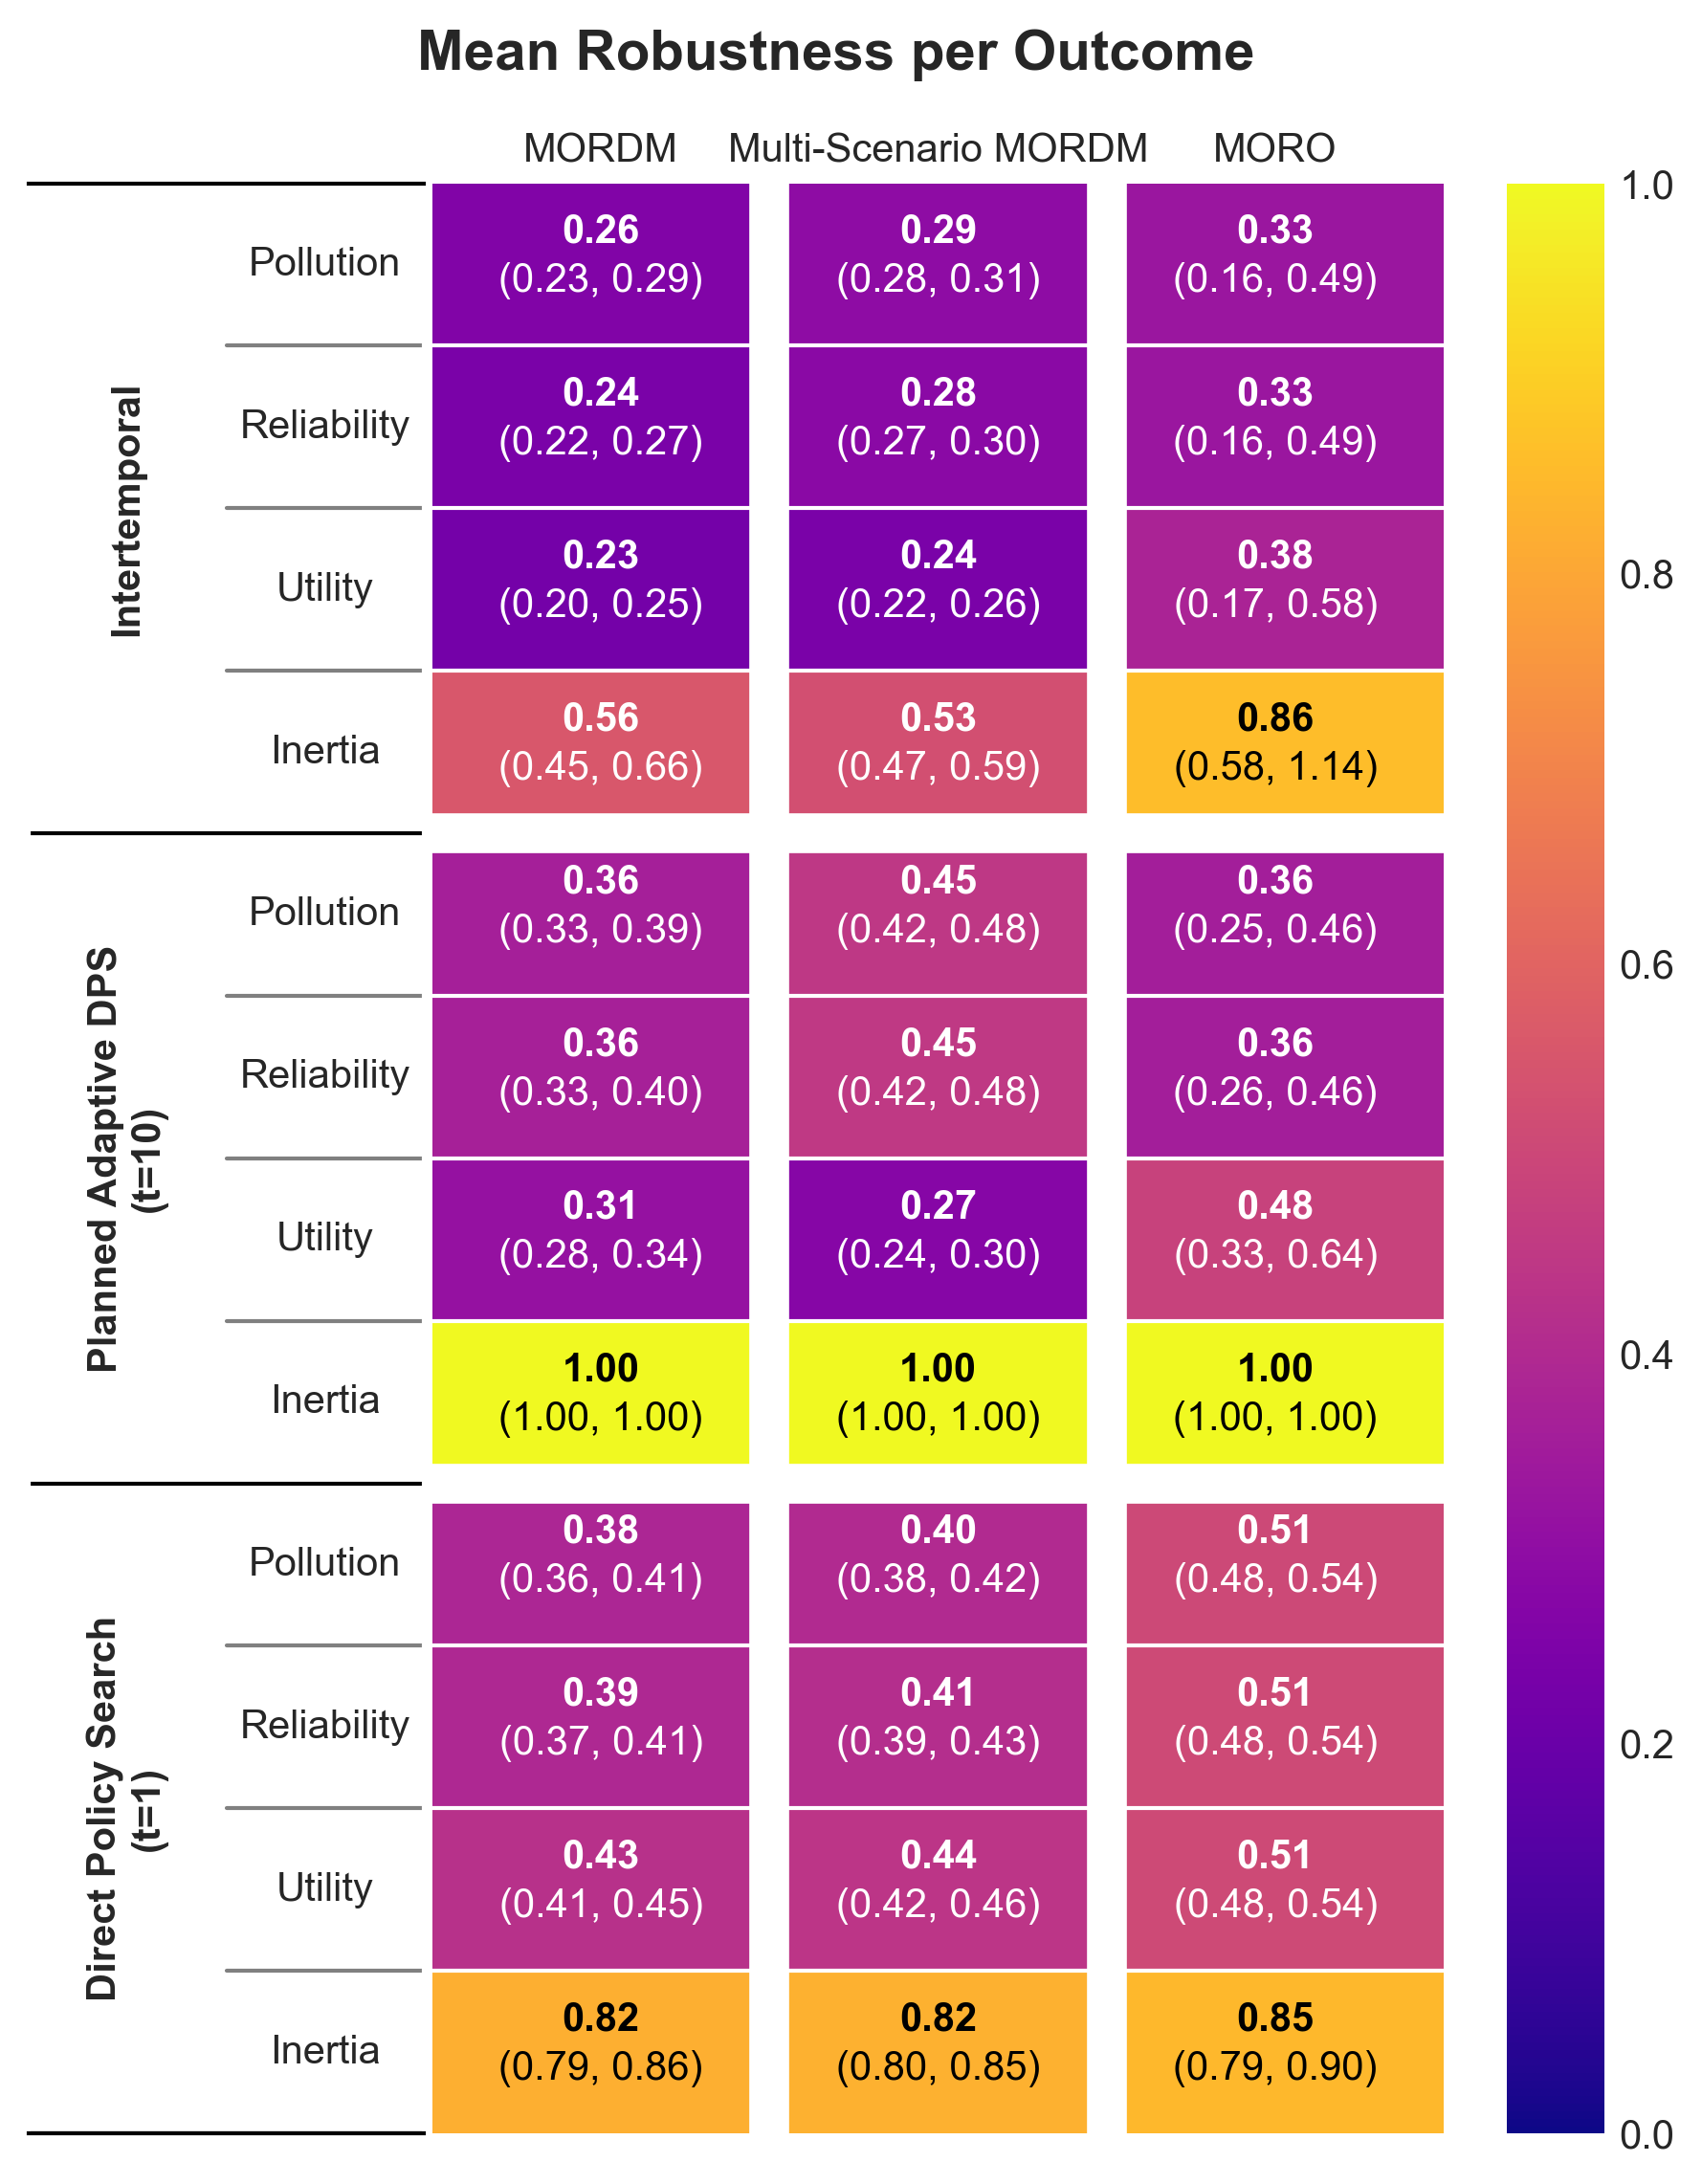
\includegraphics[width=0.8\textwidth]{compare/robust_heatmap_mean}
    \caption[Mean robustness per outcome of interest across all pairings]{Mean robustness per model variation and method pairing. This heat map is annotated to include the bounds of the 95 percent confidence interval surrounding the mean.}
    \label{fig:summary-robust-heatmap-mean}
\end{figure}

Two primary avenues for further research were also identified. First, it may be possible to mitigate the computational cost of MORO by investigating the interplay between the size of the reference scenario set used in optimization, the sampling techniques for that set, and the robustness metric used in an effort to reduce the size of the reference scenario set and therefore computational cost of that method. 

The use of the lake problem represents the second significant avenue of future research. Policy analysis and deep uncertainty literature has relied primarily on this single benchmarking problem to test and compare methods of robust decision making. The development of additional benchmarking problems would benefit both analysts and decision makers, who can leverage new problems to develop a stronger understanding of the efficacy of robust decision support methods than the use of one benchmarking problem can provide alone. 







\tableofcontents

\listoffigures
\listoftables

%% Use Arabic numerals for the page numbers of the chapters.
\mainmatter

\newpage

%% Turn on thumb indices.
\thumbtrue

\setlength{\tabcolsep}{5pt}

\part{Introduction} \label{part-introduce}
\newcounter{gapcounter}
\renewcommand{\thegapcounter}{\stepcounter{gapcounter} \Nwords{gapcounter}}

\chapter{Foundation}
\label{chapter-intro}

In 2000, the United Nations established the Millennium Development Goals \citep{UnitedNations2015}, eight goals that all United Nations members and several international organizations would work to achieve by 2015. In 2015, these goals were renewed and expanded under the name Sustainable Development Goals to a total of 17 objectives \citep{GAR2015}. Included in the list is eliminating poverty and hunger, ensuring clean water and sanitation, developing affordable and clean energy, improving infrastructure, addressing threats brought by climate change, encouraging sustainable living, and more \citep{GAR2015}. 

The manner in which to achieve each sustainable development goal can be considered a wicked problem. Characteristics of wicked problems include no definitive problem formulation, no immediate or ultimate test of a solution, and no single explanation for the cause of the problem or solution to address the problem \citep{Rittel1973}. Wicked problems also frequently demonstrate irreversible tipping point behaviors, where a rapid and significant change in a system can result from small initial changes to that system, and with no way to return to the previous behavior or system state after that tipping point is reached \citep{Gladwell2006, Lenton2013}. Tipping points in policy problems mean that solutions to wicked problems can be one-shot operations with no right for decision makers to be wrong \citep{Rittel1973}. 

Wicked problems, therefore, are subject not only to traditional types of uncertainty that can be addressed by incorporating probabilities and statistics into the analysis, but also to cognitive, strategic, and institutional uncertainties \citep{Bueren2003}. These sources of uncertainty cannot be treated as stochastic functions, but are the result of a lack of information or agreement among decision makers. This is known as deep uncertainty \citep{WalkerLempertKwakkel2013}. Given the deeply uncertain nature of achieving the UN's sustainable development goals, and of solving many other major policy problems, traditional methods of analysis and decision support almost always fall short. The traditional approach follows a predict-then-act structure, which attempts to build a single computational model that incorporates all known information, and uses that model as a surrogate for the real-world system \citep{Bankes1993}. This predictive model is then used in traditional decision analysis to find the optimal solution \citep{Weaver2013}. 

Instead of this traditional predict-then-act approach, methods of analysis have been developed to address the complexities brought by deep uncertainty that fall under the umbrella of exploratory modeling \citep{Bankes1993}. Given that analysis of deeply uncertain problems cannot reliably depend on a single description of the system under consideration, exploratory modeling uses a series of potential explanations, called computational experiments, to analyze a wicked problem and support the decision making process \citep{Bankes2002}. As wicked problems have no one right solution \citep{Rittel1973}, these computational experiments can be used explore the impact of various assumptions made related to identified deeply uncertain factors and to build a set of potential solutions that are perform well over the group of computational experiments, known as robust performance, instead of a single optimal solution \citep{Bankes2002, Kwakkel2016Compare}. 

These methods each provide a different approach to recommending satisfactory solutions to a deeply uncertain policy problem. These methods are identified as robust decision support methods in this study. Given the existence of many different approaches to robust decision support, the question, then, becomes how to determine which method is most appropriate for a specific policy problem. There is an emerging body of literature that compares robust decision support methods \citep{Hall2012, Gersonius2016, Kwakkel2016Compare, Matrosov2013a, Roach2015, Roach2016}. This study will add to that literature by comparing three different variations of Robust Decision Making, a foundational robust decision support method developed by \citet{Lempert2006}. 

\section{Robust Decision Support}
Whereas traditional predict-then-act methods focus on developing a single policy which is designed to maximize utility of the defined predictive model, robust decision support seeks a set of robust policies that achieve satisfactory performance across multiple potential future states of the world \citep{Herman2015, Popper2005, Walker2013}. Robustness can been operationalized in many ways, and each method prioritizes different policy properties, including flexibility, minimizing risk, avoiding regret, or satisficing \citep{McPhail2018}. 

Several methods of robust decision support have been developed, including decision scaling, info-gap, robust decision making, and robust optimization \citep{Herman2015}. The info-gap method focuses on quantifying how far future conditions must deviate from a most likely future state, where larger deviations from that most likely future state are what is used to indicate poor performance \citep{BenHaim2006}. However, when dealing with wicked policy problems that are deeply uncertain, it is extremely unlikely that the identified most likely future state from which to compare will be accurate \citep{Maier2016}. At the same time, decision scaling leverages decision maker feedback to reveal key uncertainties and improve projections made by existing models \citep{Brown2012}. However, decision scaling requires a system that is well-quantified \citep{Brown2012}, and pre-specified alternative policy solutions \citep{Herman2015}, both of which are not possible when addressing policy problems characterized by deep uncertainty. Each of these methods, therefore, require an analysis that incorporates significant assumptions that ignore the key characteristics of a deeply uncertain problem: no one future state of the world can be identified as more likely than another, and that there is fundamental disagreement between decision makers about the desired outcome behavior of a system.

Unlike info-gap and decision scaling, both robust decision making and robust optimization support decision making for policy problems that include deep uncertainty by minimizing the need for a priori assumptions of deeply uncertain factors.

\textit{Note: In this research, the name robust decision support methods is used to refer to the category of methods considered for comparison. This is to avoid confusion with the foundational method described in this study, which is called robust decision making.}

    \subsection{Robust decision making}
    Early efforts to address the complications brought by wicked policy problems and deep uncertainty use ensembles of models and sensitivity analysis to explore a wider spectrum of potential futures, or scenarios, and develop solutions that perform well under that wider spectrum of futures \citep{Bankes1993}. This technique of scenario-focused planning does allow for analysis to highlight the inherent variability in deeply uncertain policy problems. However, it does not include guidance on how to use that new knowledge to rank policy choices and make decisions \citep{Lempert2002}. What has become known as Robust Decision Making (RDM) builds on model-based scenario analysis to evaluate robustness of potential policy solutions over a wide range of plausible futures \citep{Lempert2002}. 
    
    RDM provides a structure for comparing previously identified policy alternatives and for discovering how changes in model properties affect each alternative's performance. That information can then be used to refine the initially identified set of policies to yield a more robust set of alternatives. This structure is iterative and interactive, allowing analysts and decision makers to work together to stress-test and refine potential policies. 
    
    The fact that RDM requires a list of promising policy alternatives from the start can prove a difficult challenge when considering problems with multiple conflicting objectives \citep{Kasprzyk2013}. As the presence of conflicting objectives is a common characteristic of wicked problems \citep{Rittel1973}, methods of decision support that incorporate the consideration of multiple objectives into a formal method are essential to the analysis of wicked problems. Combined with multi-objective evolutionary algorithms (MOEA), which aim to solve many objective problems with four or more objectives, the basic RDM method can be enhanced to support the development of promising policy alternatives despite conflicting objectives. This is known as multi-objective robust decision making \citep{Kasprzyk2013}. 
    
    Recently, multi-objective robust decision making (MORDM) was extended to address a recognized weaknesses: that the analysis must stem from a baseline scenario that is represented with a single set of input data \citep{Watson2017}. Doing so may yield invalid optimizations if the data changes significantly when compared to the original baseline scenario. Multi-scenario MORDM attempts to lower that risk by optimizing under multiple baseline scenarios \citep{Watson2017}.

    \subsection{Robust optimization}
    Different optimization methods may consider a single objective function or multiple objectives. Single objective optimization is rarely sufficient to address policy problems with deep uncertainty, as there are almost always several conflicting objectives that must be considered. Therefore, when supporting the decision making process of deeply uncertain policy problems, multi objective optimization is preferred. Several methods have been developed to support multiple objectives, including the weighted global criterion method, goal programming, Successive Pareto Optimization, and evolutionary algorithms \citep{Coello2006,Marler2004}. Each of the first three methods have significant shortcomings, including generating only one solution at a time or producing invalid results \citep{Coello2006}. Evolutionary algorithms are able to find the set of optimal solutions with one run and aren't affected by the shape of the Pareto front \citep{Coello2006}, and so will be the focus of multi-objective optimization methods that this research considers. 
    
    These traditional multi-objective optimization methods look for the Pareto optimal set of solutions, where each solution in the set is non-dominated by the other members of that set \citep{Deb2006}. However, when considering deep uncertainty, optimal solutions under one potential future can, following another possible path, lead to unacceptable outcomes \citep{Deb2006, McInerney2012}. Several studies have focused on single-objective optimization not for the optimal solution, but for a set of potentially robust solutions \citep{Branke1998, Mulvey1995, Parmee2002, TsutsuiGosh1997}. Ideas from these early approaches were then extended to develop methods for mathematical multi-objective robust optimization (MORO). The MORO method determines robustness by examining how each solution in the discovered Pareto optimal set of solutions responds to changes in key model variables \citep{Deb2006}.
    
    In the context of deep uncertainty, MORO techniques have been used as a small step within existing decision support methods. For example, to configure tipping points of dynamic policies developed using the adaptive robust design method \citep{Hamarat2013} or to determine the most promising sequence of pathways from a larger set defined through dynamic adaptive policy pathways analysis \citep{Kwakkel2015}. multi-objective optimization techniques, however, have not yet been codified into a formal method for decision support. This leads to the first gap that this research will address. 
    
    \begin{researchbox}{Research Gap \thegapcounter}\label{gap-moro}
        Robust optimization techniques have not yet been integrated into an RDM-based decision support process in literature. 
    \end{researchbox}

    \subsection{Comparing MORDM and MORO}\label{gap-comaprativework}
    MORDM has been well established in literature, as have the techniques that MORO requires. Though each method has the common goal of determining a set of policy alternatives that are maximally robust across many potential futures, the path each follows to determine a set of promising policy alternatives differs. MORDM seeks robust solutions by searching for solutions that perform best under uncertainty conditions defined by a base reference scenario and then determining robustness of those alternatives by examining the performance of each promising alternative under a much wider range of uncertainty conditions \citep{Kasprzyk2013}. In contrast, MORO focuses on determining the most robust solutions possible by incorporating robustness into the initial search process through evaluating a potential policy across a small ensemble of uncertainty settings and returning those policies which have the highest robustness for further analysis \citep{HamaratLoonen2014}. There are several articles that compare concepts held by MORDM and MORO to other decision support methods. \citet{Hall2012} and \citet{Matrosov2013b} compare RDM with the Info-Gap methodology and \citet{Roach2015} compares robust optimization with Info-Gap. \citet{Kwakkel2016Compare} compares RDM with a method called Dynamic Adaptive Policy Pathways, which leverages robust optimization techniques to build its recommendations. These articles all compare methods by leveraging real-world case studies. Additional literature compares concepts held by several methods \citep{Dittrich2016, Herman2015, Maier2016}. However, this existing body of work does not yet compare these two methods directly or with respect to policy problems characterized by tipping points, as many wicked problems are. This represents the second gap that this research will address.
    
    \begin{researchbox}{Research Gap \thegapcounter}\label{gap-comparativework}
        There is a lack of comparative analysis of the identified robust decision support methods that can help decision-makers determine which method is most suitable to their needs.
    \end{researchbox}

\section{Policies Developed with Robust Decision Support Methods}\label{gap-policies}
Robust decision support methods have been used to develop policies with different implementation structures, especially with respect to the type of adaptation considered. These methods have each been used to recommend sets of robust policy options that are static and do not change over time \citep{Sozuer2016,Kasprzyk2013}. Each has also been used to develop sets of robust policies that are adaptive, both through automatic responses to adaptation triggers and from manual adjustments at predefined points in time \citep{HamaratLoonen2014, Kwakkel2015, Trindade2017}.

Despite the flexibility of these robust decision support methods to develop policy alternatives following many different implementation structures, the comparative literature that exists and is discussed in \cref{gap-comaprativework} have generally focused on only one policy implementation structure at a time. This is the third and final gap in literature that this research will address.

\begin{researchbox}{Research Gap \thegapcounter}\label{gaptwo}
    Existing work that compares decision support methods focuses on one specific case and one policy implementation formulations, and not the impact of varying policy formulations on the results of analysis.
\end{researchbox}

\section{Thesis Structure}
This thesis will be structured in the following way. First, the remainder of \cref{part-introduce}: Introducing the Problem will establish the goals and methods used in this study (\cref{chapter-research}), and will provide a review of the concepts that are fundamental to answering the identified research question (\cref{chapter-review}). \cref{part-develop}: Design and Development will establish the implementation details for the methods and problem formulations identified in \cref{part-introduce}. Included in this part will also be a description of the points of comparison that will be used in the comparison, which can be found in \cref{dev-comparisons}. Finally, \cref{part-analysis}: Analysis and \cref{part-discussion}: Discussion, will describe the results of analysis, including comparisons as described in \cref{dev-comparisons}) and conclusions that can be made based on these results. \cref{part-discussion} will also answer this study's key questions in \cref{chapter-conclusion}, the implications of those answers for analysts and decision makers in \cref{chapter-reflection} and discuss future avenues of research related to the problem identified and results that were generated in \cref{chapter-futurework}. 

\chapter{Research Definition}
\label{chapter-research}

\section{Research Question}\label{research question}

The gaps identified in \cref{chapter-intro} provide the foundation for this masters thesis. The goal will be to develop a framework for and perform a comparative analysis that considers the trade-offs of different methods of decision support. Considerations will include trade-offs in computation, communication to decision makers, similarity of results, and method complexity. Therefore, the research question that will be answered is the following: 

\begin{researchquestion}{Research Question}\label{research-question}
    What are the trade-offs between different methods of decision support when considering a wicked problems and varying policy implementation structures? 
\end{researchquestion}

\section{Approach}
To answer the research question, three identified methods of robust decision support (MORDM, multi-scenario MORDM, and MORO) and their handling of three variations of a wicked policy problem that features tipping point characteristics will be considered. Therefore, a multiple case study approach will be used, which provides a structure for developing a deeper understanding of a theoretical framework or methodology, in this case robust decision support methods, through the analysis of a case or cases of interest \citep{Edwards1998}. The goal of following a structured case study approach and of considering a single case will be to develop generalized conclusions of method trade-offs that can be applied to wicked policy problems with tipping point characteristics \citep{Seawright2008}.

A comparative approach will be incorporated into the case study to ensure rigor in when comparing methods. The comparative method, as defined by \citet{Pennings2006} provides several guidelines to ensure rigor in a comparative analysis. This includes defining the important concepts and points of comparison, establishing the cases that will be used for comparison, and carefully developing causal statements from the established comparisons \citep{Pennings2006}. 

    \subsection{Case Selection}
    Case selection involves seeking a representative sample of cases that include variation along the key dimension under consideration \citep{Seawright2008}. In this case, the key dimension considered is the policy implementation structure of a system. To facilitate method comparison, a highly stylized problem known as the lake problem will be used. This problem features tipping point behavior and is commonly used in existing policy analysis research and bench-marking work. To test the response of each robust decision support method to different policy implementation structures, this stylized problem will be varied to support three levels of policy intervention: a policy with pre-determined and static decisions, a planned adaptive policy that is updated periodically based on a predetermined number of time steps, and a dynamic adaptive policy that is updated after every time step. 

    \subsection{Caveats}
    There are a few recognized pitfalls of using a case study approach to research that must be considered and guarded against. Case studies are often accused of a lack of rigor \citep{Yin2012}, so it will be imperative to monitor the data collection, method application, and results analysis to ensure that rigor is maintained. Second, generalization of results from the selected cases to the wider population can prove problematic \citep{Zainal2007}. Careful selection of the case considered and clear establishment of the research objectives can increase confidence of generalizing the results found \citep{Seawright2008, Yin2012}.

\section{Supporting Questions} \label{def-supporting-questions}
To support the primary research question, several sub-questions will be addressed. This study and, therefore, identified sub-questions, will be structured to follow the commonly accepted IMRAD research framework of Introduction, Methods, Results, And Discussion \citep{Nair2014}. Leveraging such an established framework for research provides structure and helps to ensure that this work is understood and accepted by other researchers.

\begin{enumerate}
    \item \textbf{Introduction}\newline
    Beyond the research definition, this will include establishing a thorough background for the key concepts identified in the research definition
        \begin{itemize}[label={--}]
            \item How is robustness defined in policy analysis? 
            \item What are the origins of the robust decision support methodology?
            \item How have stylized policy problems been leveraged in previous research? 
            \item Does the lake problem incorporate deep uncertainty tipping point behavior? 
            \item What policy implementation structures are commonly recognized in literature?
        \end{itemize}
        
    \item \textbf{Methods}
    Included in this part of the study are the implementation details for each method and problem variation. The framework for comparison is also included in the methodology.  
        \begin{itemize}[label={--}]
            \item What are definitions of the lake problem that represent the three essential types of policy implementation?
            \item How can robustness be determined for each selected robust decision support method?
            \item What are the implementation details for each robust decision support method identified for this study?
            \item What are the points of comparison which should be considered during analysis? 
        \end{itemize}
    
    \item \textbf{Results}
    Results include both an individual analysis of each method and problem variation pairing, as well as a comparison following the framework established in Methods. 
        \begin{itemize}[label={--}]
            \item What are the results from each pairing of robust decision support method and variation of the stylized policy problem?
            \item Based on the points of comparison defined in Methods, how do the results of each pairing compare? 
        \end{itemize}

    \item \textbf{Discussion}
        \begin{itemize}[label={--}]
            \item Based on the points of comparison and definitions of robustness that have been developed, what trade-offs exist between methods and how do methods respond to the different problem variations?
            \item How can the results from this analysis be generalized to other problems and analyses? 
        \end{itemize}
\end{enumerate}

\section{Research Methods}\label{research methods}
Continuing to follow the IMRAD format, this section will discuss methods used for each step in the research process. 

\subsection{Part 1: Introduction}
An extensive review of the literature about each of the robust decision support methods selected will establish the origins and intended implementation of each. Flow charts will be leveraged to identify the specific order of execution for each method. Additional literature review will explore how robustness can defined, both generally in the context of decision making and policy analysis and specifically for individual robustness metrics. The stylized problem and policy structure variations will also be developed from a review of previous applications of the lake problem and research regarding possible policy structures.

\subsection{Part 2: Method}
Development of the identified variations of each stylized policy problem will use Cython, a high performance programming language implemented as a superset of the Python language that allows for the compilation of extremely efficient C code. Using such a high performance language will reduce computing time for these computationally-intensive decision support methods by speeding up the most commonly used process: the problem itself.

This step will also define how each robust decision support method will be executed. The research required to identify proper algorithms for each step of a method will be completed with further literature review of the relevant concepts. Finally, methods will be implemented by leveraging open-source libraries wherever possible to avoid duplicated work and to leverage already well-tested functionality. This will be supplemented with code using Cython when there is potential for a beneficial reduction of processing time. By using Cython for coding needs whenever possible, additional computational power beyond what is available for student use will be minimized as much as possible.

As this research intends to compare multiple methods of robust decision support, it is important to establish how each method is evaluated and how those evaluation methods can be compared. Therefore, literature will be reviewed to determine and quantify points of comparison that will be tracked during execution of each pairing.

\subsection{Part 3: Results}
The results for each method and problem variation will first be determined in isolation, both through data analysis and visual interpretation of results. Visualizations will be built using python-based graphing libraries like Matplotlib and Seaborn. Comparison points established earlier will be then be considered, using mathematical formulas and visualizations where applicable.

\subsection{Part 4: Discussion}
The final step will involve several methods of communication. First, visualizations that summarize the significant results of comparison. Second, the development of a comprehensive thesis that describes the results of each step of research as described in the research definition. All word processing activities will use Latex and relevant templates. The thesis will be submitted to the TU Delft repository and will be made available for download. Finally, code developed for both policy problem variations and for method implementations will be made available through GitHub.

\section{Research Flow}\label{research flow and scheduled}
The research flow found in Figure \ref{fig:flow} provides a guide for the work completed to answer the identified research question. Notice that points of comparison are defined prior to method specification in practice to limit bias when defining metrics, which aims to add validity to the comparison performed in this study. For clarity, however, these metrics will be defined after method and problem development in text.

\begin{figure}[!h]
    \begin{center}
        \captionsetup{width=0.6\textwidth}
        
        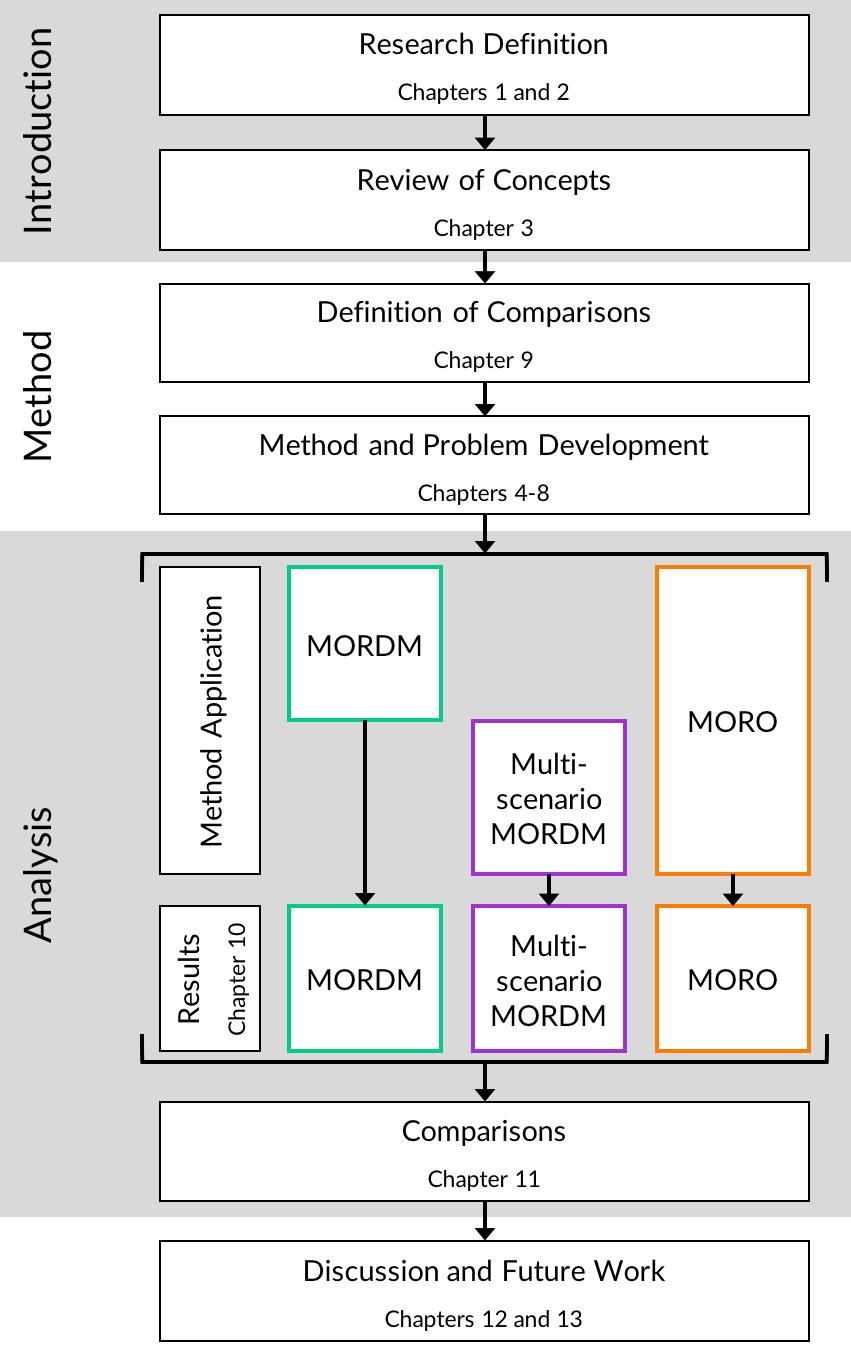
\includegraphics[width=0.6\textwidth]{research-flow}
        \caption{Structure of the work involved this research project}
        \label{fig:flow}
    \end{center}
\end{figure}

\chapter{Review of Concepts}
\label{chapter-review}

\begin{abstract}
    The purpose of this chapter is to provide background knowledge and definitions of key concepts that are essential when addressing the identified research question. First, the concept of deep uncertainty is codified in \cref{review-uncertainty}. \cref{review-robustness} investigates recognized definitions of robustness in literature. Then, \cref{review-methods} explores the foundations and key concepts for each of the selected robust decision support methods. Finally, the stylized policy problem identified in the research definition is discussed in \cref{review-problems}, along with the relevant policy implementation structures.
\end{abstract}

\newpage

\section{Deep Uncertainty}\label{review-uncertainty}
Uncertainty is generally defined as the state of something not being known or not being completely certain \citep{def:uncertain}. Uncertainty due to a lack of information, even despite growing scientific knowledge has long been discussed in philosophy and scientific research \citep{Tannert892}. Modern research into the concept began with Frank Knight, who was one of the first to distinguish types of uncertainty: knowable uncertainty or Knightian risk, which can be converted easily into effective certainty through probabilities or other means, and true uncertainty or Knightian uncertainty, which cannot be measured or described effectively \citep{Knight1921}. Similarly, Edward Quade developed two categories of uncertainty: stochastic and real. Stochastic uncertainty is similar to Knightian risk and can be quantified using probabilities, while real uncertainty is similar to Knightian uncertainty and is the result of unknowable futures or actions \citep{Quade1989}. Knightian or real uncertainty provides the foundation for a concept called deep uncertainty. The formal definition of deep uncertainty that has become commonly accepted in policy analysis research was developed by \citet{Lempert2003}: 

\begin{conceptbox}\label{def:deepuncertainty}
    Deep uncertainty exists in policy problems when analysts do not know or cannot agree on one or more of the following three elements:
    \newline
    \begin{enumerate}[leftmargin=*]
        \item The model(s) that correctly describe relationships between key system elements that will shape the future
        \item The probability distributions that best represent uncertainties in key system elements
        \item The manner in which to rank the desirability of potential outcomes
    \end{enumerate}
\end{conceptbox}

Given the nature of wicked policy problems as established in \cref{chapter-intro}, deep uncertainty is an unavoidable obstacle to the decision support process. Whereas traditional policy analysis focuses on using a predict-then-act model to find the optimal solution, the presence of deep uncertainty means that accurate prediction and determination of what an optimal solution is become extremely difficult, if not impossible. When the focus for problems with deep uncertainty is on the search for an optimal solution, assumptions must be made in several areas: 

\begin{itemize}
    \item To determine all possible future scenarios and of their likelihood
    \item To define the probabilities and value ranges that describe identified uncertain variables
    \item To understand and operationalize what criteria an optimal solution must meet. 
\end{itemize}

Each of the elements required for optimal search, therefore, directly contravene the properties of deeply uncertain problems defined here. Because the correctness of a model that describes potential futures cannot be agreed upon, there is no way to concretely determine future scenarios and their likelihood. And continuing to the second point, the presence of deep uncertainty means that is no agreement on specification of uncertainties and their quantitative values. So, there can be no certainty about the values of identified sources of uncertainty. And finally, because there is a lack of agreement on what makes a potential solution more desirable than another, there can be no concrete definition of what makes a solution optimal. Instead, policy making must focus on a different evaluation method that looks to satisfy stated goals instead of optimize the system at hand. 

\section{Robustness}\label{review-robustness}
As the search for an optimal solution is recognized as an impossible task when faced with deeply uncertain problems, policy makers have instead looked to an alternate mechanism to analyze the goodness of potential solutions: robustness \citep{Maier2016}. The concept of robustness has a long history in engineering, economics, supply chain management, and many other fields \citep{Capano2017, Maier2016}. Engineering considers a robust system as one who is able to maintain functionality in the presence of failure of a part of the system \citep{Capano2017}. In biological robustness is seen as the ability for a system to maintain development despite external perturbations \citep{Jen2003}. Robustness of organizations is viewed as the ability of that organization to maintain its function through changing internal and external conditions \citep{Capano2017}. Common among these definitions is that robustness of a system of any type exists when that system is able to maintain core functionality in the face of external change. This concept of robustness will be used as the foundation for robustness in policy analysis. 

Robustness in policy analysis can be defined in multiple ways. First, it is possible to define robustness at a system level, where the system is most often represented as a model that describes the uncertainties, policy levers, relationships, and desired outcomes that is used to analyze the problem of interest. Robustness of a system can be defined similarly to robustness of natural systems. A robust system has the ability to maintain its functions despite changes in internal or external factors \citep{Capano2017}. Defined in this way, robustness becomes distinct from other possible measures of system performance: resilience, stability, and adaptability. A robust system is able to maintain functionality but is not required to maintain the same state, where a resilient or stable system is able to maintain the same state. And in contrast to robustness, adaptability can be considered a property of a lever or policy that helps a system maintain robustness \citep{Capano2017}. 

Robustness can also be defined for a policy, which is generally represented as a set of possible lever values. This definition of robustness will be the focus of this research. The following is a general definition of robustness as defined for potential policies of a specific system: 

\begin{conceptbox}\label{def:robustness}
    A robust policy is one that performs well across a variety of possible future states of a system, due to both internal and external changes \citep{Herman2015,Kasprzyk2013,Matrosov2013a,WalkerLempertKwakkel2013}. 
\end{conceptbox}

Instead of searching for the optimum solution, by seeking a set of solutions based on robustness, the search process will better avoid finding solutions that are overly sensitive to changes in uncertain parameter values. It is possible for the optimum solution of a system to belong to the set of solutions that are considered robust (which is known as a super-robust solution). However, it is much more common that the robust solution to have lower performance than the optimum solution given a set of uncertain parameter and decision lever values \citep{Sniedovich2016}. This is known as \textit{the price of robustness} \citep{Bertsimas2004}. 

Robustness of a policy can be analyzed from multiple perspectives: resistance to change, avoidance of change, recovery from change and adaptability in response to change \citep{Durach2015,DeGoede2013,Twomey2012}. Because there are several facets to a policy's robustness, there exists many established robustness metrics, each prioritizing a different facet of robustness. Calculation of each of these metrics generally involve the same three elements: determination of the different decisions that could be made, outcomes of interest or performance metrics, and the scenarios or possible future states of the world that will be considered. Robustness metrics may determine performance as an absolute calculation or relatively to other policies. Each metric also employs differing levels of risk aversion: include more extreme scenarios in calculations to have a higher level of risk aversion. Finally, each metric has a different method of combining robustness calculations across scenarios for a specific policy option, including mean, standard deviation, skewness, or kurtosis \citep{McPhail2018}.

The following are a selection of robustness metrics that have been identified in previous policy and system analysis literature. The first group of methods listed below can be considered classical robustness metrics who use the absolute value of a performance measure to determine robustness, and report a robustness value with the same units as the performance measure under consideration \citep{McPhail2018}. The benefit of methods that directly communicate system performance mean that it is extremely simple to communicate the elements that make a policy alternative robust. 

\textbf{Minimax (strict robustness):} a worst-case approach that seeks the best performance under the worst case analyzed. Worst case scenarios are often black swan types of event \citep{Taleb2007}, where a black swan event is one that is rare, unexpected, and has a significant impact on a system. Because black swan events are inherently rare, they do not represent a good estimate of actual performance. Minimax is therefore an extremely conservative approach to determining robustness of a policy. The value of such a conservative approach depends on the problem under consideration. If costs of a worst case scenario are extremely high, then it makes sense to consider that worst case scenario in robustness calculations. However, under many other conditions, a worst-case scenario does not lead to catastrophically high costs, so determining a policy's robustness based on performance under the worst-case scenario may lead to unnecessarily expensive or conservative solutions. 

\textbf{Maximax:} follows a similar principle as the minimax criterion, but focuses instead on best case performance instead of worst case \cite{McPhail2018, Rosenhead1972}. By focusing the extreme positive range of values for an outcome, the maximax metric may ignore catastrophic conditions in the worst case scenario, leading to significant negative problems for decision makers. 

\textbf{Hurwicz optimism-pessimism rule:} representing the middle ground between minimax and maximax, Hurwicz rule involves a weighted average between the two metrics, with the weighting up to the decision maker to determine robustness \citep{Rosenhead1972}. Because the weighting is left up to decision makers, they are able to customize this metric according to their desired level of risk aversion \citep{McPhail2018}. 

\textbf{Laplace's principle of insufficient reason:} by assigning equal weight to all possible scenarios, robustness is determined as the mean of all values for an outcome \citep{Rosenhead1972}. This results in a robustness metric that has an average level of risk aversion. 

Other methods in this category include maximin, percentile-based skewness and peakedness, and mean-variance. 

The methods listed next calculate robustness based on relative performance, but produce outputs with the same units as the considered performance metric, making communication of robustness with decision makers a straightforward process. In this case, the robust option is one in which minimizes the maximum regret \citep{McPhail2018}

\textbf{Minimax Regret and 90th percentile minimax regret:} seeks to minimize regret with respect to the worst-case performance (or the 90th percentile of the worst case). Similar to the minimax metric, these metrics are conservative and have high risk avoidance.

\textbf{Undesirable deviations:} unlike minimax regret, this metric determines robustness as the deviation of the mean of the lower 50th percent of performance values from th median performance, given the set of performance measures over an ensemble of scenarios \citep{Kwakkel2016Robust}. This method results in a level of risk aversion that is lower than that found in minimax regret and 90th percentile regret, but still maintains a relatively high level of risk aversion \citep{McPhail2018}

Instead of determining robustness that indicate actual system performance, the final robustness calculation considered here indicates only whether the system is performing satisfactorily or not. Satisficing metrics use the value of performance measures directly, but will report a relative robustness value that indicates whether performance is satisfactory \citep{McPhail2018}. There are many satisficing metrics available, the most common of which is described below: 

\textbf{Starr's domain criterion:} defines robustness based on the number of scenarios in which a performance measure meets a decision maker's defined threshold \citep{Hadka2015}. Because the threshold for performance is determined by the decision maker, she is able to customize this metric according to her preferred level of risk aversion.

Common among these metrics is that each is defined with respect to some value or set of conditions that must be established based on the problem that is being analyzed. Therefore, a policy's robustness value is only valid under conditions specific to the system being analyzed and to the definition of robustness used. At the same time, selection of the appropriate metric to use is based primarily on decision maker objectives, but may also depend on limitations of the method that is used for analysis. Combining the wide variety of possible robustness metrics, each of which measure robustness in a different manner, the subjectivity of metric selection, and the fact that robustness values are only valid in the specific problem and analysis context under which they are calculated, it becomes difficult to asses the real-world robustness of a system, given a specific policy implementation. 

Several studies have been completed that compare different robustness metrics given a specific problem \citep{Giuliani2016, Herman2015, Kwakkel2016Robust, Roach2016}. These studies have generally concluded that each robustness metric indicates a different facet of the robustness of a potential policy. This makes it difficult to compare robustness across different metrics and can lead to confusion between decision makers, who must determine how to use the analysis and robustness values in their decision-making process. \citet{McPhail2018} propose a framework that categorizes the different robustness metrics based on several factors, including required inputs, method of calculation, unit of output, and level of risk aversion. This taxonomy aims to assist decision makers in determining the most appropriate metric to use when analyzing their own problems. And while this guidance may provide a stronger foundation with which to select a specific robustness metric, selection of a specific metric will still have a significant impact on the policy recommendation process. 

Given that it is impossible to identify a single optimum policy in the case of a deeply uncertain problem and armed with the knowledge required to define a policy's robustness instead of it's  absolute performance, a prescriptive method to determine policy alternatives and their robustness is required.

\section{Robust Decision Support Methods}\label{review-methods}
The search for robust solutions instead of the optimal one requires assessment of  different potential solutions over a large ensemble of possible future states of the world, also known as scenarios. Exploratory Modeling and Analysis (EMA), is a technique that can be used as a foundation for methods that support this process. This technique advocates the use of computational experiments that describe the range of potential future states of the world of a system and to use those experiments to explore the behavior of that system in response to different policy settings \citep{Bankes1993}. EMA techniques have integrated into the robust decision support methodology, which is descried next. 

    \subsection{Robust decision making}\label{review-rdm}
    Analysis of deeply uncertain wicked problems brings along with it several requirements. First, that policies should be analyzed with respect to robustness and not optimality (which was discussed in \cref{review-robustness}). Second, that the set of potential futures cannot be represented as a small number of possibilities (given the large amount of uncertainty that is frequently influenced by multiple input variables, it is generally impossible to codify a short list of possible futures for a problem), but has to instead be described using large ensembles of potential futures, with the number of scenarios stretching anywhere from a few hundred to several million. Analysis of these problems must also lead to results that can be clearly communicated to decision makers, to ensure that any conclusions are not just used to inform decisions, but are interpreted correctly. Furthermore, wicked problems characterized by deep uncertainty commonly involve multiple decision makers and always include conflicting views on model and input specification, and on output ranking. Because of these factors, any decision making process must be iterative, providing the opportunity for feedback from decision makers and model or policy refinement based on that feedback \citep{Tsoukias2008}. 
    
    \citet{Lempert2003} proposes a prescriptive and systematic method to support decision making of problems with characteristics similar to a wicked problem known as robust decision making (RDM) that attempts to address many of the factors listed above. The proposed method involves an iterative process of model and policy specification, computer aided computational experimentation that involves the generation and execution of a large ensemble of scenarios that span the defined uncertainty space, development of interactive visualizations, and decision maker input and refinement based on the results of computational experimentation and generated visualization \citep{Lempert2006}. For the purposes of this research, a description of the method flow can be found as \cref{fig:rdm-flow}. 

    \begin{figure}[ht]
        \centering
        \captionsetup{justification=centering}
        
        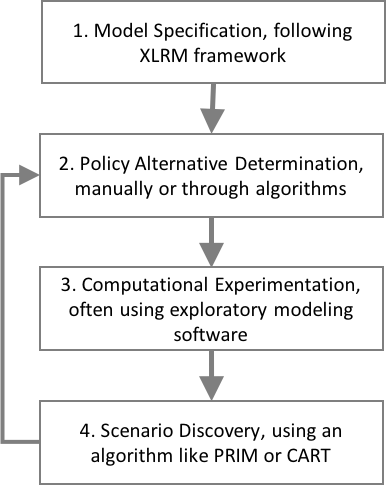
\includegraphics{rdm-flow}
        \caption{Robust Decision Making Process}
        \label{fig:rdm-flow}
    \end{figure}
    
    The first step of any formal analysis must be to organize any relevant information into a usable form. In the case of RDM, this step is referred to as model specification. To accomplish this, \citet{Lempert2003} proposes a 4-category structure with which to organize model elements, known as the XLRM framework. "X" refers to the exogenous uncertainties that are outside of the control of decision makers but still impact behavior of the system being considered. Variables that are controlled by decision makers are categorized under "L", also known as policy levers. The desired outcomes of interest are categorized as measures, or "M". Finally, relations ("R") describe how each of the elements in the "X", "L", and "M" categories relate to one another. Together, the items described by each of the 4 categories become the model that will be used for the remainder of analysis.

    \begin{figure}[ht]
        \centering
        \captionsetup{justification=centering}
        
        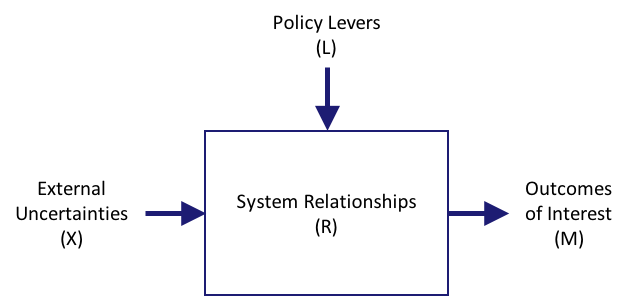
\includegraphics{xlrm}
        \caption{The XLRM Framework \citep{Kwakkel2017}}
        \label{fig:xlrm}
    \end{figure}
    
    As a part of the structuring of data and information, the second step of the RDM process involves identifying policy alternatives, also known as candidate strategies. The selection process can manifest in many different ways. Decision makers may contribute a set of initial strategies that will be considered \citep{Lempert2006}. Alternatively, analysis can leverage the specified model to determine policies based on sensitivities to identified sources of uncertainty or decision levers through a traditional sensitivity analysis.
    
    In step three, the XLRM specification is used to build a diverse ensemble of possible future states of the world (SOWs), or scenarios, that span the uncertainty space specified in the first step. The set of future SOWs are used to determine how the defined policies may react to a wide variety of possible futures. This stage generally involves the use of software to both build the ensemble of scenarios and to apply that ensemble to the set of policy options to build a data set that evaluates the potential effectiveness of a policy given the XLRM problem definition. 

    Once the evaluation data is built through computational experimentation in step 3, that information is used to calculate policy robustness and to discover vulnerabilities in the existing policy options based on the identified robustness measure (possible robustness metrics were discussed in \cref{review-robustness}, but RDM traditionally favors a satisficing measure \citep{Matrosov2013b}). The process of searching for vulnerabilities is known as Scenario Discovery. PRIM (the Patient Rule Induction Method) is typically identified as the most suitable scenario discovery method for RDM, as it produces simple rules that accurately determine the factors (both uncertainties and policy settings) which contribute to poor performance \citep{Lempert2006}. This information is used to refine both the model and policy options in an iterative process until the analyst and other decision makers reach a policy option or set of options that they can implement to address the problem. 
    
    Together, these four steps formed an iterative process that is one of the first attempts to develop a prescriptive method to guide the decision making process under conditions of deep uncertainty. The RDM method as it stands falls short in one key way. First, when there is deep uncertainty present in an analysis, there are going to be many decision makers involved who don't agree on the proper XLRM specification and who will have conflicting objectives \citep{WalkerLempertKwakkel2013}. Though the RDM process does support decision maker interaction throughout the process, it does not codify a formal mechanism for determining different policy options when faced with conflicting objectives \citep{Kasprzyk2013}. Other methods of decision support have been developed that build on the RDM structure but seek to address this shortcoming, which will be reviewed next. 

    \subsection{Multi-objective robust decision making (MORDM)}\label{review-multi}
    Building on the foundation of RDM, \citet{Kasprzyk2013} propose a decision support method called multi-objective robust decision making (MORDM), which provides a structure for managing a wide spectrum of decision maker perspectives and conflicting objectives. \cref{fig:mordm-flow} indicates how MORDM has been adapted from RDM. The most significant change is the introduction of a formal process to determine potential policy alternatives in step 2 through the application of a multi-objective evolutionary algorithm (MOEA). The MOEA searches for potential policy solutions and ranks them based on performance of the system at a base reference point (which is determined with decision maker input). A policy alternative is added to the Pareto non-dominated set of alternatives if its performance in the base reference scenario is not outperformed by another member of that set. By leveraging an MOEA, the MORDM process is able to quantify outcomes of interest that represent conflicting objectives and account for the conflict directly in this search phase. 
    
    \begin{figure}[ht]
        \centering
        \captionsetup{justification=centering}
        
        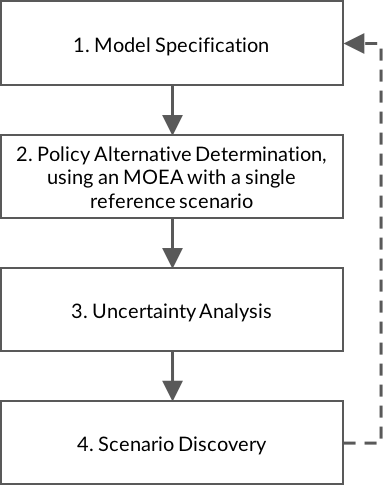
\includegraphics{mordm-flow}
        \caption{Multi Objective Robust Decision Making Process}
        \label{fig:mordm-flow}
    \end{figure}

    The MORDM method also codifies the process with which to help select a preferred solution from the set of solution alternatives generated with the MOEA, through uncertainty analysis, scenario discovery, and interactive visualizations \citep{Kasprzyk2013}. After model specification and an MOEA search for policy alternatives, the performance of the list of alternatives is tested under the recognized deep uncertainties through a process known as uncertainty analysis. This involves building a set of alternative future states of the world by sampling across the set of uncertainty parameters, a specified sampling method. Though there are many techniques available, from Monte Carlo to full and partial factorial, \citet{Kasprzyk2013} recommends using Latin Hypercube Sampling, which ensures that each member of the uncertainty set is represented evenly across the sampled set of SOWs \citep{Mckay1979}. 
    
    The data gathered from exercising each alternative policy over the set of SOWs provides the required information to perform a robustness analysis, in which a robustness metric is selected in a similar manner to the RDM method and robustness of each policy is calculated on a per-objective basis. This information is communicated through interactive visualizations that decision makers can leverage examine the robustness of policy alternatives and to better understand the trade-offs that exist between conflicting objectives. At this point, candidate strategies are selected by the decision maker for further analysis, through the scenario discovery process. Scenario discovery in the MORDM method is similar to that in the RDM method, where candidate policy alternatives are tested to determine potential vulnerabilities \citep{Bryant2010}. The MORDM method also supports an iterative structure wherein the information gathered in the uncertainty analysis and scenario discovery process can be used to refine potential policy alternatives. However, as MORDM leverages an MOEA to determine alternatives, any refinements occur at the model specification level, where new information can be used to adjust the uncertainty space or to influence the set of available decision levers, instead of the policy alternative determination phase (see \cref{fig:rdm-flow} and \cref{fig:mordm-flow}). 
    
    Because of the changes MORDM has made to the RDM process, the space for decision makers to impact the decision making process has also changed. Whereas RDM involves the decision maker in the early stages of the process to determine initial policy alternatives, by combining an MOEA with software-enabled uncertainty analysis and scenario discovery, the policy alternative selection process is not influenced by assumptions from decision makers until after the initial set of policy alternatives have been discovered and tested against a large ensemble of potential future SOWs. Given that problems analyzed with either RDM or MORDM methods are characterized by deep uncertainty, where there is conflict about the best way to achieve success, removing conflicting biases from the initial policy alternative selection process and focusing on optimizing over the set of conflicting objectives defined in the XLRM specifications directly can lead to the discovery of more robust solutions that might not have been considered otherwise. 

        \subsubsection{Applications of MORDM}\label{review-mordm-apps}
        Since its inception in 2013, the MORDM method has been tested and applied to several cases in policy analysis literature. As the MORDM method was designed to address challenges faced by problems relating to environmental systems management \citep{Kasprzyk2013}, many of the problems analyzed also fall within this domain (though this is not a requirement to apply MORDM). Though this is not an exhaustive list of all applications of MORDM, it provides an overview of the uses of MORDM and some of the extensions to the method that have been developed since its inception.
        
        In the initial proposal of MORDM, \citet{Kasprzyk2013} demonstrates the MORDM method through a case that considers options for dealing with the water supply in the Lower Rio Grand Valley in Texas, USA and applied a robustness metric that focuses on performance in the worst-case SOW (minimax). In this case, the application of the MORDM method was able to recommend a small and manageable set of policy alternatives, each of which includes robustness calculations for the conflicting outcomes of interest. 
        
        \citet{Herman2014} uses a case about water management in the Research Triangle region of North Carolina to demonstrate and extend the MORDM method. Proposed extensions include to more explicitly handle analysis of deeply uncertain problems with multiple interacting decision makers and to demonstrate how to use the lessons learned in scenario discovery to improve robustness by managing uncertainties that affect policy robustness. The analysis in this research led to the discovery of key vulnerabilities of the system under consideration, and indicated which elements of a comprehensive are common among the identified robust methods and will ensure the greatest chance for success \citep{Herman2014}. This application leverages a satisficing robustness metric that seeks the best performance over a range of possible futures, as recommended in the initial RDM literature \citep{Lempert2007}. Satisficing in this case is defined as the "fraction of sampled states of the world in which a solution satisfies all performance requirements" \citep{Herman2014}. 

        Finally, \citet{Trindade2017} uses an application of the same water management problem to extend the policy alternative search phase of the MORDM method; a satisficing definition of robustness similar to \citet{Herman2014} is also used. \citet{Trindade2017} determines if a policy alternative belongs in the non-domianted set of alternatives through each policy's performance under a random scenario that is changed every generation of the MOEA-based search. This random scenario is culled from a set built by sampling the uncertainty space. The goal of this effort is to provide a broader reference space with which to determine a policy's robustness earlier in the analysis. Policy alternatives discovered using a broader set of test scenarios in the search phase of the MORDM method were discovered to have a higher level of robustness. The set of policy alternatives was also more diverse with the modified MOEA search \citep{Trindade2017}. Together, these elements can provide decision makers with more detailed analysis of vulnerabilities and trends in recommended policies. 
        
        The use of different robustness metrics while applying MORDM indicate that the method is not tied to a specific metric. In fact, the MORDM method does not provide any guidance about the most appropriate robustness metric, leaving it to the decision makers and analysts to determine for themselves. Given the wide variety of robustness metrics that exist which test so many different facets of robustness (see \cref{review-robustness}), the chosen metric can have a significant impact on the recommendations made by the MORDM method. The enhancement made to the search phase of MORDM by \citet{Trindade2017} indicate that the proposed application of MOEA search in MORDM is not always sufficient to discover many valid robust policy alternatives. 

    \subsection{Multi-scenario MORDM}
    The MORDM method made significant strides toward developing a more effective process for handling policy problems characterized by deep uncertainty where there are multiple decision makers who are unable to agree on system details and solution objectives. The key to MORDM is the use of multi-objective evolutionary algorithms, which are responsible for determining potentially promising policy alternatives. 
    
    Based on the MORDM method as established by \citet{Kasprzyk2013}, the outcomes of a potential policy are compared with others based on a single base reference scenario. Policies that perform better than those belonging to the existing non-dominated set under the uncertainty settings established by the base scenario will be added to the non-dominated set, with conditions of deep uncertainty being included later in the analysis \citep{Eker2018}. \citet{Watson2017} recognize that this means the non-dominated set of options will be based on a single reference point and may not lead to policies that are robust if conditions change. This conclusion is similar to that of \citet{Trindade2017}, discussed in \cref{review-mordm-apps}. Remember that \citet{Trindade2017} addresses this by introducing multiple reference scenarios simultaneously to the selection of the scenario used to compare success of policy options. 
    
    In contrast, the multi-scenario MORDM method proposed by \citet{Watson2017} proposes to perform multiple iterations of the MOEA search process using distinct reference scenarios built based on the results of a sensitivity analysis in the traditional MORDM method, with the goal of building a set of policy alternatives that cover a more diverse range of decision levers, in an effort to discover policy alternatives that perform well under even the most extreme conditions. 
    
    \begin{figure}[ht]
        \centering
        \captionsetup{justification=centering}
        
        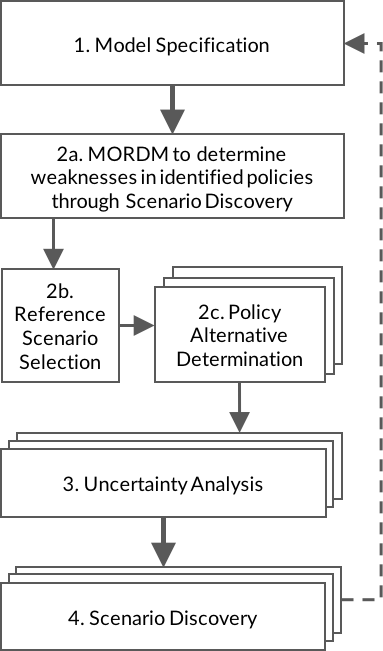
\includegraphics{multi-flow}
        \caption{Multi-Scenario MORDM Process}
        \label{fig:multi-flow}
    \end{figure}
    
    As \cref{fig:multi-flow} demonstrates, the key difference between MORDM and multi-scenario MORDM lies in the search for policy alternatives. The complete and distinct sets of non-dominated policies built from the search involving each reference scenario are all considered throughout the remainder of the method: uncertainty analysis and scenario discovery. 

    Given the proposal to repeat the search for policy alternatives with multiple reference scenarios, the most influential decision in this method will be the selection of reference scenarios. The initial proposal, which is illustrated in \cref{fig:multi-flow} is to use the results of sensitivity analysis performed during the course of MORDM-based analysis as boundaries with which to select the reference scenarios from \citep{Watson2017}. Through this method, \citet{Watson2017} are able to conclude that the use of multiple reference scenarios lead to the discovery of a more diverse set of policy alternatives that perform well under deep uncertainty to consider.
    
    The number of scenarios to select is left to the analyst to determine. By selecting a wide range of scenarios to use as reference points, it is more likely to discover a more diverse set of robust policy options. However, analysis is often limited by computational capabilities and other factors, which means that analysts should search for only a small number of reference scenarios \citep{Eker2018}. There are several criteria that can be considered during the selection process, including internal consistency, diversity of outcome indicators, extremeness, and policy relevance, which may be combined or considered separately depending on goals of the analysis or decision maker preference. \citet{Eker2018} use this information to develop an alternative method of reference scenario selection that is designed for the purpose of finding reference scenarios that, when used in the MOEA search, will lead to more robust solutions, focusing on policy relevance and maximum diversity (where policy relevance is defined as scenarios that lead to outcomes in the lower half of the scenario space and the diversity criterion is based on that which was defined by \citet{Carlsen2016}). \citet{Eker2018} also apply a random approach by selecting a number of scenarios randomly across the uncertainty space, with no consideration for policy relevance or diversity. 

    After applying each mechanism to an intertemporal version of the lake problem (for more details about the lake problem, see \cref{review-problems}), the results using policy relevant reference scenario selection mechanism were shown to lead to a more diverse set of policy alternatives, as well as larger variety of trade-offs in robustness metrics \citep{Eker2018}. The same analysis did not find a signficant difference between the results for the policy relevant scenario selection mechanism and the random mechanism, with both leading to similar increases policy alternative diversity and robust outcome trade-offs \citep{Eker2018}. 
    
    As multi-scenario MORDM is such an new method, there are currently no other applications in literature. Much remains to be learned with respect to the impact of differing scenario selection mechanisms or the effect of using a different number of scenarios on the diversity and robustness of discovered policy alternatives.

    \subsection{Multi-objective robust optimization (MORO)}
    Robust optimization has its roots in mathematical optimization of functions and systems. Traditional optimization algorithms seek the maximum (or minimum) solution(s) generated from a mathematical system and specified input space. In decision making, system optimization commonly refers to determining optimum values for levers which decision makers can use to create the conditions required for a system to reach the targeted outcome. As discussed in \cref{review-robustness} these optima can be unstable and sensitive to even small changes in parameter values. When the system under consideration includes uncertainty, let alone the deep uncertainty present in wicked problems with tipping point characteristics, an optimum that is sensitive to changes in parameter values may easily lead to outcomes that do not hit the desired target. In these cases, a robust solution is desired over an optimum one, which must be accounted for in the optimization process. Early attempts to combine a desire for robustness with a search for optimality occurred in the 1960s \citep{Dorato1966} with the consideration of insensitive optima, and 1970s with the development of an algorithm that seeks the optimum values of levers under worst-case performance settings, given a set of uncertain input parameters \citep{Soyster1973}. It was not until the 1990s, however, that what is now known as robust optimization began to take shape \citep{Sozuer2016}. 
    
    A robust optimization algorithm seeks solutions to a problem that perform reasonably across all potential future states of the world and performs best in worst-case scenarios. Two primary forms of robust optimization have been developed. Deterministic robust optimization uses numerical techniques to determine function optima explicitly. In situations with deep uncertainty, however, it is not possibly to explicitly define all robustness constraints and function variables. In this case, a randomized approach or simulation optimization approach is used \citep{Beyer2007}. Given that wicked problems with tipping point characteristics will always include deep uncertainty, the consideration of robust optimization in this research will focus on simulation optimization.
    
    Robust optima in uncertain models are found through direct evaluation. Robust solutions to the objective function are determined by sampling across the uncertainty space, which can be accomplished in three primary ways \citep{Beyer2007}:
    
    \begin{enumerate}
        \item Monte-Carlo strategies: this involves averaging the objective function values across a sample set of the uncertainty space. Sets of uncertainty values are determined through one of a variety of sampling techniques, including Latin hypercube, Monte-Carlo, and full- and partial-factorial. This method of simulation optimization quickly becomes computationally expensive. 
        \item Meta-model approach: generally used to reduce the computational cost of optimization, a meta-model is carefully constructed to represent the model of interest. Results of optimization using the meta-model are then generalized to estimate optimization results of the original model \citep{Zhou2017}
        \item Optimization using objective function directly: instead of calculating robustness values from the objective function, this method proposes to use the values of the objective function directly to compare policy alternatives \citep{Beyer2007}
    \end{enumerate}
    
    Evolutionary algorithms have been used in combination with Monte-Carlo strategies and noisy optimization to more efficiently obtain robust solutions to a model’s objective function. Evolutionary algorithms are discussed in more detail in \cref{step2-moea}. 

    Previous literature has applied robust optimization techniques as a small step in a larger method of designing policy solutions for a problem characterized by deep uncertainty. \citet{HamaratLoonen2014} uses multi-objective robust optimization as a method of fine-tuning tipping points during adaptive policy making. \citet{Kwakkel2015} makes use of multi-objective robust optimization in the development of Dynamic Adaptive Policy Pathways (DAPP). In this case, robust optimization is used to assess candidate pathways and find the most robust options. Extensions of the MORDM method have approached a multi-objective robust optimization implementation in the search phase by considering more than one reference scenario. In one case, the method continues to determine a policy alternative's dominance through its performance with respect to a single reference scenario at a time \citep{Watson2017}. The closest extension of MORDM is by \citet{Trindade2017}, who, in the context of MORDM, proposes the use of multiple states of the world to calculate robustness and determine whether an alternative is selected during the search phase. However, that approach is specific to the problem under analysis and is not formalized into a prescriptive method for decision support. 
    
    \begin{figure}[ht]
        \centering
        \captionsetup{justification=centering}
        
        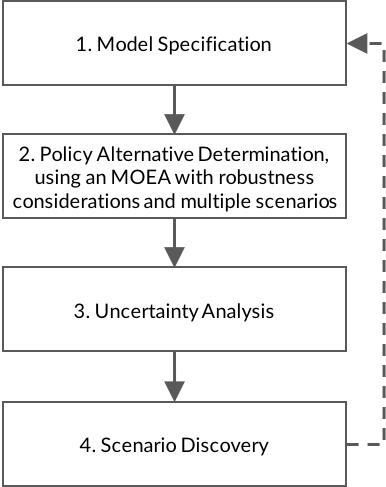
\includegraphics{moro-flow}
        \caption{Multi-Objective Robust Optimization Process}
        \label{fig:moro-flow}
    \end{figure}
    
    This research proposes a multi-objective robust optimization methodology that follows the structure of RDM and can be used as the primary method for analysis to determine the set of robust policy options to a deeply uncertain wicked problem with multiple conflicting objectives. Model specification follows the same XLRM format as was described in \cref{review-rdm}. Robust optimization takes place in the MOEA-based policy alternative determination phase of the method, as illustrated in \cref{fig:moro-flow}. In this stage, policies are compared based on the outcomes of defined robustness metrics, leading to the Pareto optimized set of policies based on robustness. This comparison is compatible with many robustness metrics, depending on the interests of decision makers or the analyst. To enable the calculation of a robustness metric, each policy identified in the MOEA search is evaluated against a set of pre-specified scenarios. The outcomes calculated are then used to determine robustness for each outcome according to the formula of the specified robustness metric. 

    %    A different implementation of the policy alternative determination process is described by \citet{Beh2017}, in which a meta model is used to evaluate robustness, which is determined using a single robustness function. However, by using the model under analysis directly, and by considering each outcome of interest as an independent element of robustness, the search phase is better able to both fully capture the dynamics of the model and consider conflicting objectives, making the robust optimization method proposed in this research a more direct method of incorporating robustness into the search phase of analysis. 
    
    After the search phase is complete, the result is a set of Pareto non-dominated policy solutions that are already considered robust against the set of evaluation scenarios specified for the search. These policies are further tested in uncertainty analysis and scenario discovery to both determine robustness against a significantly larger set of scenarios and find remaining vulnerabilities that can be used to refine the model specification in a new iteration of the analysis. 

    \subsection{The fundamental difference between MORDM, multi-scenario MORDM, and MORO}

    Each of the methods described, MORDM, multi-scenario MORDM, and MORO, are based on the foundations of robust decision support: the RDM method. Though there are many similarities between the three methods, there is one fundamental difference. As highlighted in \cref{fig:diff-flows}, each method takes a different approach to the policy alternative determination phase of the method.
    
    \begin{figure}[ht]
        \centering
        \captionsetup{justification=centering}
        
        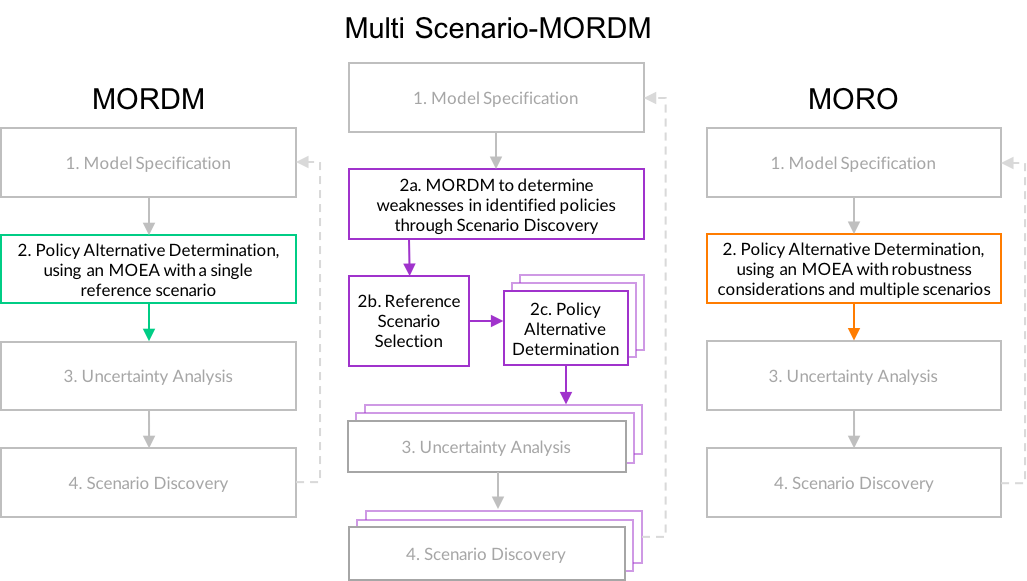
\includegraphics[width=\textwidth]{diff-flows}
        \caption{Comparison of robust decision support method structures}
        \label{fig:diff-flows}
    \end{figure}

    From left to right, the methods increasingly integrate robustness into the policy alternative determination process. MORDM selects policies based on outcomes of interest alone. While multi-scenario MORDM also selects policies based on outcome values, it performs the search using multiple reference scenarios identified from within the vulnerable uncertainty space as determined in scenario discovery of MORDM, thereby introducing small robustness considerations into the search phase. And finally, instead of using outcome values, MORO selects policies by testing each against a pre-defined set of scenarios and using the robustness metric for each outcome, which even more directly brings robustness considerations into the search phase of the method.
    
    As the model specification, uncertainty analysis, and scenario discovery processes are all constant across the three methods, this research will be examining the impact of considering robustness in the policy alternative determination step of an RDM-based method for decision support. 

\section{Problem and Policy Configuration}\label{review-problems}
This section will provide background on the stylized problem used in this study. It will also explore commonly used policy implementation structures, in an effort to select a subset of implementation structures that can be used to test the analytic power of each robust decision support method.

    \subsection{The lake problem}
    In order to compare the methods described in \cref{review-methods}, there must be a usable problem that is representative of the desired behavior. The type of wicked problem under consideration has been identified as including deep uncertainty, a threshold point of no return, where behavior of the system changes dramatically, and the consideration of many decision makers with multiple conflicting criteria. What is known as the shallow lake problem, a common reference problem in policy analysis research, incorporates all of these characteristics. This problem, developed into a policy analysis problem initially by \citep{Carpenter1999}, is a highly stylized decision problem in which a town must decide the amount of pollution to release into a nearby shallow lake over time. As \cref{fig:lake-model} illustrates, this hypothetical problem involves two sources of pollution: anthropogenic pollution generated by the town through industrial and agricultural waste, and natural inflows that are uncontrollable and come from the environment. There is also a natural outflow process based on the capability of the lake to recycle resources that is capable of naturally reducing pollution over time in the lake \citep{Hadka2015}. 

    \begin{figure}[ht]
        \centering
        \captionsetup{justification=centering}
        
        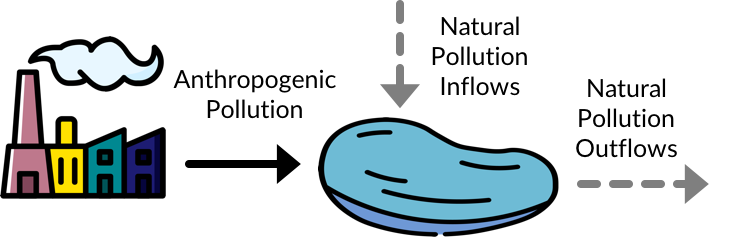
\includegraphics[width=\textwidth]{lake-model}
        \caption{Illustration of pollution flows in lake model}
        \label{fig:lake-model}
    \end{figure}
    
    Through the inflow and outflow processes, the lake's water quality will shift between two states \citep{Carpenter1999}: 

    \begin{itemize}
        \item Oligotrophic equilibrium, with low algae production, high oxygen content, and therefore high fish counts and drinking-water quality
        \item Eutrophic equilibrium, with high levels of algae production and therefore lower fish counts and drinking-water quality. A lake in the eutrophic state reduces the economic benefit of the lake to the nearby town. 
    \end{itemize}

    \begin{figure}[ht]
        \centering
%        \captionsetup{justification=centering}
        
        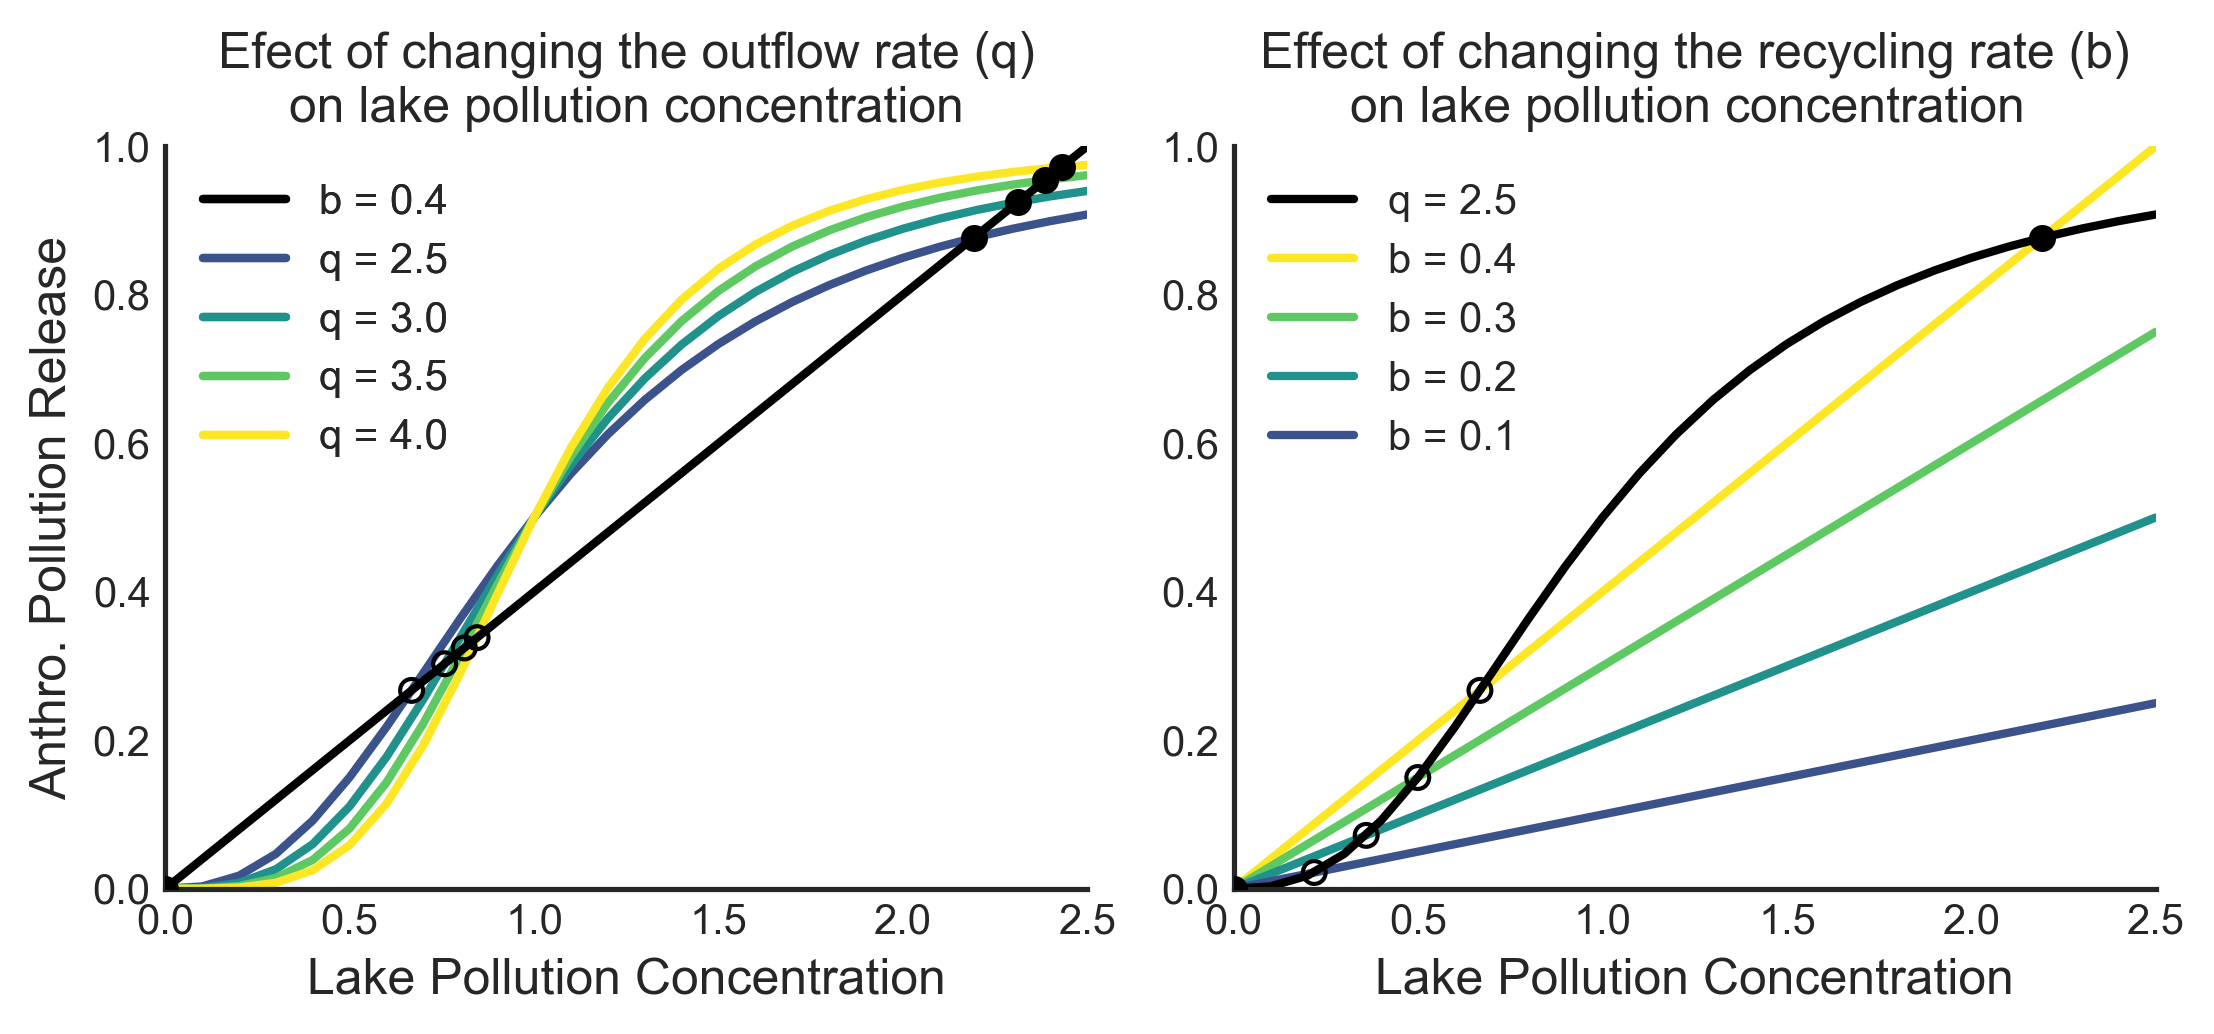
\includegraphics[width=\textwidth]{tippingpoint}
        \caption[Tipping point behavior integrated into the shallow lake problem.]{Illustration of the tipping point behavior present in the lake problem. These plots show the impact of changing the properties that allow the lake to naturally reduce the pollution level on the lake's pollution concentration. Hollow circles represent the unstable equilibrium or tipping point, of the system, while filled circles highlight the stable oligotrophic (at point (0,0) in both plots) and eutrophic equilibrium. Based on a plot found in \citet{Quinn2017}.}
        \label{fig:tippingpoint}
    \end{figure}
    
    Pollution levels are determined through \cref{eq:pollution}, where \textit{X} represents the concentration of pollution in the lake, \textit{a} is the anthropogenic pollution input for the time period, \textit{Y} refers to the natural inflows of pollution, \textit{q} indicates the recycling rate at which pollution is removed from the lake through recycling by the lake's sediment, and \textit{b} refers to the loss of pollution from the lake through natural outflows. The exact specifications for each of the parameters are based on the lake model developed by \citet{Quinn2017}. 

    \begin{equation}\label{eq:pollution}
        X_{t+1} = X_{t} + a_{t} + Y_{t} + \frac{X_{t}^{q}}{1+X_{t}^{q}} - bX_{t}
    \end{equation}

    Because the lake problem is designed to include tipping point behavior, the transition between the two states may be rapid and result from even a small change in inflow levels. When the critical threshold of pollution concentration is surpassed, the trend transitions toward eutrophic equilibrium, making impossible to return to a healthier oligotrophic equilibrium without active human intervention to reduce the pollution level in the lake \citep{Quinn2017}. This is visualized in \cref{fig:tippingpoint}. Both panels indicate that the more pollution a lake is able to remove naturally, the higher the lake's tipping point is, making it easier to avoid the point of no return and a eutrophic equilibrium. 
    
    The characteristics of the lake problem also allow it to incorporate competing desires between maximizing a town's economic productivity by maximizing anthropogenic pollution release, and minimizing negative impacts on the lake's water quality to ensure a healthy environment for fishing, leisure, and other activities \citep{Ward2015}. 
    
    There are several benefits from using this stylized problem over a case study based on specific real-world properties. First, the behavior described by the lake problem can be considered similar to the behavior of many other real-world issues that include a balance between generation of sources that can negatively impact a system with the loss of benefits when that system is negatively impacted. This dynamic is especially common in environmental problems like climate change and other pollution-related issues \citep{Carpenter1999}. Second, by using a relatively straightforward model, it is easy to catalog assumptions and omissions, which enables more rigor when assessing the effectiveness of different robust decision support methods. And finally, by using a stylized problem that has been used in research before, there is a stronger foundation for comparison and validity of results with respect to that problem and its characteristics. 

    \subsubsection{Sources of uncertainty}
    The lake problem that is used for this research includes five sources of uncertainty. As indicated in \cref{eq:pollution}, $b$ and $q$ indicate the ability of the lake to remove pollution through natural processes. Two additional sources of uncertainty relate to the natural inflows of pollution to the lake from the environment, where the inflow, $Y$ is represented as a function of $\mu$, the mean of natural inflows for the lake, and $\sigma^{2}$, the standard deviation of natural inflows \citep{Quinn2017}. The remaining source of uncertainty $\delta$, represents the future discount rate of utility. 

    \subsubsection{Objectives}
    Along with the five sources of uncertainty, the lake problem identifies four conflicting objectives: maximum pollution level, utility of the release policy to the town, reliability of the policy, and policy inertia. The multi-objective form of this problem was introduced by \citet{Singh2015} and further developed by \citet{Ward2015}, with the goal of introducing objectives that exemplify the conflicts that occur with a diverse group of decision makers and a problem characterized by deep uncertainty.
    
    \textbf{Maximum Pollution (minimize)}: Some decision makers are seeking to ensure that the maximum pollution level reached in the lake is kept to as low a value as possible. This objective represents the perspective of environmental regulators who strive to maintain the health of the lake \citep{Singh2015}.
    
    \textbf{Reliability (maximize)}: Representing the interest of key decision makers who are especially concerned with keeping the lake in an oligotrophic state, because they depend on it for income, recreation, or some other purpose. Reliability captures desire of decision makers to keep the lake below the critical pollution threshold. At the same time, in contrast with the maximum pollution objective which strives to strictly minimize pollution, a policy that has high reliability is also accepting of a small amount of pollution, as long as it remains under that critical threshold \citep{Singh2015}.

    \textbf{Utility (maximize)}: To contrast the objectives that relate the goals common among environmental regulators, utility represents the interests of the town's agriculture and industry, with the goal being to maximize the utility of a policy for those decision makers. This objective naturally conflicts with the objective of minimizing the pollution level in the lake, providing a valuable dynamic for robust decision support analysis \citep{Ward2015}. 
    
    \textbf{Inertia (maximize)}: Capturing the interests of the lake manager, this objective refers to the stability of the pollution release amount over time. As dramatic changes in pollution will require large infrastructure investments, it is in the lake manager's interest to maintain a steady level of pollution release over time \citep{Quinn2017}. 

    \subsection{Policy implementation structure} \label{review-structure}
    Given a deeply uncertain problem with several sources of uncertainty and multiple conflicting objectives, the next step of analysis is to establish a strategy or policy that helps decision makers reach their objectives. There are two approaches to policy development, each of which are fundamentally different and have varying internal characteristics \citep{Maier2016}.
    
    \textbf{Static}: A fixed strategy that is fixed and is not adjusted despite changes in the system. A static solution can be one decision that is being made at the start of the time horizon being considered. Alternatively, a static policy can consist of multiple decisions that are executed at predetermined points in the time horizon.
    
    \textbf{Adaptive}: A flexible strategy that responds to changing conditions or increased knowledge about the current or future state of the world. Adaptive policies can be implemented in different ways: 
    \begin{itemize}
        \item A static adaptive approach, in which there is a static policy in place that remains fixed and is supported by contingency actions to help keep the system in a good state. 
        \item A dynamic approach to adaptation, in which the available set of policy options itself changes based on changing conditions or new knowledge about the future state of the world. 
    \end{itemize}

    The comparisons made in this research will consider three policy structure alternatives, based on those identified above.

    \textbf{Intertemporal}: Also known as open-loop control, this variation of the lake problem has been used in research several times and involves a series of pre-determined static decisions made every time-step \citep{Hadka2015,Quinn2017,Singh2015,Ward2015}. This option represents a strictly static approach to solving the lake problem. 

    \textbf{Direct Policy Search}: Representing the other extreme in policy structure, direct policy search (DPS), or closed-loop control. Instead of building a policy that defines anthropogenic pollution release levels, the DPS structure involves optimizing a set of parameters that form a state-aware pollution release rule. This control rule is used to update the level of pollution released at every time-step, giving this policy structure the ability to quickly respond to changes in system conditions. The DPS structure has also been used as a part of the lake problem in research before \citep{Quinn2017}. 
    
    \textbf{Planned Adaptive DPS}: Given that both the intertemporal and DPS policy structures adapt the pollution release every time period, they do not necessarily represent real-world decision strategy, where it takes time to implement changes. Therefore, this research is proposing a third policy structure that follows the same fundamental structure of the DPS policy, but updates the level of pollution that is released every time step every N time steps (instead of every time step, as in traditional DPS), where N is a number set by the decision makers or policy analysts. 


\part{Methods} \label{part-develop}
\chapter{Step 0: Foundation} \label{dev-step0}

\begin{abstract}
    Part 2 of this dissertation defines specific implementations of each method considered: MORDM, multi-scenario MORDM, and MORO. It also specifies the value ranges of uncertainties and levers, practical definitions of the outcomes of interest, and the functional structure of each problem variation: intertemporal, DPS, and planned adaptive DPS. 
    
    This first chapter provides a background on how the implementations of both methods and problem variations were developed, and will describe the specific definition of robustness used across this analysis, which will be referenced in more than one step of the analysis.
\end{abstract}

\begin{figure}[h]
    \centering
    \captionsetup{justification=centering}
    
    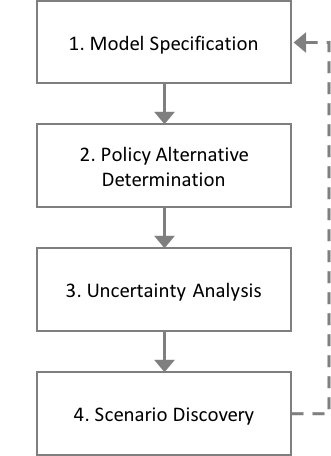
\includegraphics{structure-step0}
    \caption{Basic RDM analysis structure}
    \label{fig:structure-step0}
\end{figure}

\newpage

\section{Implementation Structure}
The implementation structure will follow the fundamental flow of the RDM process, with each of the next four chapters describing a step of an RDM-based decision support process, found in \cref{fig:structure-step0}. \cref{dev-step1} contains the model specification for all three variations of the lake problem. \cref{dev-step2} defines the policy alternative determination process for each of the three methods. As this step is where the key methodological difference lies, \cref{dev-step2} contains critical information that differentiates each method. Next, \cref{dev-step3} describes the process of uncertainty analysis, including the method of determining how robust each policy alternative is considered. The final step in the RDM process is scenario discovery, which is discussed in \cref{dev-step4}. Finally, this part concludes by establishing the points of comparison that will be considered in \cref{dev-comparisons}.

\section{Definition of Robustness}\label{step0-robust}
The review in \cref{review-robustness} described several options for determining robustness of policies under conditions of deep uncertainty. Traditionally, the desired robustness metric specification is determined through conversations between analysts and decision makers to ensure that goals of decision makers are being met. Often, the involved parties will consider multiple robustness metrics for the same analysis to provide a broader picture of the robustness of each policy \citep{Quinn2017}. 

To facilitate the comparison of results across methods in this study, a single common definition for robustness will be used: the domain criterion measure. The domain criterion measure, a satisficing metric, will provide the most effective and straightforward way to focus on policies that ensure minimum thresholds of performance are met when considering conflicting objectives. This metric is suitable wherever robustness is used in all three methods of analysis under consideration. 

As a reminder, domain criterion satisficing is defined as the fraction of all considered future states of the world (SOWs) in which a threshold of performance is met \citep{Starr1963}. This results in a metric value between 0 and 1, where 0 indicates that no set of uncertainty values produced an outcome that met the defined threshold given a specific policy configuration, and 1 indicates perfect performance. The threshold values and goal for each outcome can be found in \cref{table:robust-thresholds}. 

\begin{table}[h]
    \centering
    \captionsetup{width=0.55\textwidth}
    \caption{Robust threshold values for each outcome of interest of the lake problem}
    \label{table:robust-thresholds}
    
    \setlength\arrayrulewidth{1pt}\arrayrulecolor{white}
    \rowcolors{2}{odd-row-blue}{even-row-blue}
    \begin{tabularx}{0.55\textwidth}{l|l|l}
        \rowcolor{tudelft-dark-blue!80}
        \color{white}\bfseries Outcome  &  \color{white}\bfseries Goal  &  \color{white}\bfseries Threshold  \\ 
        \hline
        Pollution Level   & Minimize      & Critical Pollution Level            \\ \hline
        Utility           & Maximize      & \multicolumn{1}{|r|}{0.75}          \\ \hline
        Inertia           & Maximize      & \multicolumn{1}{|r|}{0.99}          \\ \hline
        Reliability       & Maximize      & \multicolumn{1}{|r|}{0.8}           \\
    \end{tabularx}
\end{table}

These values are generally based on previous research that has developed and tested the lake model \citep{Quinn2017, Singh2015}, save the pollution level. One difference relates to the threshold for the pollution level. Previous research has used a static value for the pollution threshold when determining robustness. This study proposes using the critical pollution level as defined by \citet{Quinn2017} as the threshold for the lake's pollution level.

\subsection{Minimizing the maximum pollution level}
The first outcome of interest, indicating the interests of environmental protection groups, is defined as the fraction of SOWs whose maximum level of pollution remains under the critical pollution threshold (the tipping point after which it is impossible to return the lake to al oligotrophic state without manual intervention). The critical pollution threshold is defined in \cref{eq:critp}, where b and q refer to specific values of the uncertainty inputs to the lake model, b and q, and X represents the level of pollution under consideration \citep{Quinn2017}. This function produces two intercepts, the first of which represents the critical pollution threshold, $Pollution_{crit}$. 

During execution, one experiment out of the set of N states of the world (which is a pairing of an SOW and a set of lever values that constitute a policy) generates T releases of pollution into the lake, the maximum value of which is returned. The robustness metric is then calculated by determine the fraction of experiments for which the pollution level remains under the critical P threshold. 

\begin{equation}\label{eq:critp}
    \frac{X^{q}}{(1+X^{q})}-b*X
\end{equation}

\subsection{Maximizing utility}
Also known as expected economic benefits for the town (through industry and agriculture), utility of robustness is determined as the fraction of experiments for which their average utility level is above the threshold defined in \cref{table:robust-thresholds}. The first component of this metric is to determine the utility of a policy in an experiment, known as the discounted economic benefits. This value is determined for every year in the time period of interest. Discounted economic benefit for one year of the simulation run is defined in \cref{eq:utility}, and involves two parameters from the set of uncertain parameters to be discussed in \cref{dev-step1}: $\alpha$ and $\delta$. The vector of expected utility values calculated using \cref{eq:utility} are then averaged to get a single value that is used to calculate robustness. 

\begin{equation}\label{eq:utility}
    \sum_{t=0}^{T-1}\alpha*a_{t}*\delta^{t}
\end{equation}

\subsection{Maximizing inertia}
As discussed in \cref{review-problems} the lake manager has an interest in maintaining as stead a release rate of pollution as possible, to avoid unnecessary expenses that occur from rapid changes in release levels. Therefore, the third robust outcome of interest is to maximize the average inertia of a policy. Like utility, inertia of an policy and for an experiment is first calculated for every time step involved. The mean of that vector of values is what is used to determine inertia-based robustness. Inertia for a single time step in an experiment is determined with \cref{eq:inertia}. 

\begin{equation}\label{eq:inertia}
    \sum_{t=1}^{T-1}\phi_{t}, \text{where } \phi_{t} = \begin{cases}
    1 & |X_{t}-X_{t-1}| < 0.01| \\
    0 & \text{otherwise}
    \end{cases}
\end{equation}

\subsection{Maximizing reliability}
The last robust outcome of interest to define is reliability. As reliability indicates the likelihood that a policy will lead to pollution levels remaining under the critical p threshold, the lake manager and other parties interested in keeping the lake healthy are seeking policies in which a high fraction of policies yield potential futures in which the pollution level stays consistently below the critical pollution level, and so it is another maximizing objective. The reliability of a single experiment is determined as the average of the reliability measures for each time step, shown as \cref{eq:reliability} \citep{Ward2015}.

\begin{equation}\label{eq:reliability}
\sum_{t=1}^{T}\theta_{t}, \text{where } \theta_{t} = \begin{cases}
1 & X_{t} < P_{crit} | \\
0 & \text{otherwise}
\end{cases}
\end{equation}
\chapter{Step 1: Model Specification}\label{dev-step1}

\begin{abstract}
    The model specification stage is common across the three methods identified for comparison. It involves using an XLRM structure to develop a model or models of the system under consideration. There are details of each of the policy structure alternatives identified that will lead to unique XLRM structures for each of the three versions of the lake problem. The specification will explain the model specification in the following order: exogenous uncertainties (\cref{step1-X}), decision levers (\cref{step1-L}), outcomes of interest (\cref{step1-M}), and relations (\cref{step1-R}), or XLMR. This is different from the commonly written order of XLRM, but is done for clarity and to ensure that each component of the model is specified before their relations are described. 
\end{abstract}

\medskip

\begin{figure}[h]
    \centering
    \captionsetup{justification=centering}
    
    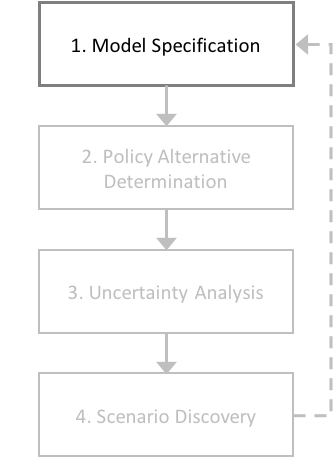
\includegraphics{structure-step1}
    \caption{RDM Structure - Step 1}
    \label{fig:structure-step1}
\end{figure}

\newpage

\section{General Approach}
The first step to each of the identified robust decision support methods is problem specification. This involves building a computer-based model of the problem identified by decision makers. Model development for the three methods compared in this study require an XLRM-based specification structure. The XLRM structure requires the identification of inputs, through uncontrollable uncertainties (X) and adjustable decision levers (L), outcomes of interest or performance measures (M), and relations (R) that describe how different combinations of input values lead to different potential future states of the system under consideration. 

Without an existing well-structured definition of a problem, the XLRM specification is developed through review of the relevant background information and existing literature. The analyst uses that information in combination with conversations among a variety of decision makers and subject-matter experts to ensure that all relevant data and views are incorporated into the defined system \citep{Lempert2003}. In addition to identifying the structure of the problem under consideration, the specification must operationalize decision levers and uncertainty parameters through identifying value ranges, probability distributions, or other means. 

Through research and discussion, a specification of the problem at hand will be developed, which will be used to determine a set of potentially robust policy alternatives. 

\section{The Lake Problem}
For the purposes of this study, a well-researched, well-defined and commonly referenced highly-stylized policy problem is used known as the lake problem. Using an existing well-defined and accepted policy problem allows the focus of the comparison to remain on the two factors under consideration: the impact of the robust decision support method and of the policy implementation structure. 

As such, literature that has previously defined and tested the specification and implementation of this problem is leveraged to build the specification of the lake problem for this study. This section will describe the details following the XLRM structure defined for all three methods of robust decision support. 

    \subsection{"X": Exogenous Uncertainties}\label{step1-X}
    There are five sources of uncertainty in the definition of the lake problem used for this study. The uncertainty ranges and base values have been selected based on the most commonly used settings in literature \citep{Carpenter1999,Eker2018,Hadka2015,Quinn2017,Ward2015}. The specific settings for each uncertainty parameter are found in \cref{table:uncertainties}. 

    \begin{table}[ht]
        \caption{Exogenous uncertainty settings}
        
        \label{table:uncertainties}
        
        \setlength\arrayrulewidth{1pt}\arrayrulecolor{white}
        \rowcolors{2}{odd-row-blue}{even-row-blue}
        \begin{tabularx}{\linewidth}{l|X|l|l}
            \rowcolor{tudelft-dark-blue!80}
            \color{white}\bfseries Name     &      \color{white}\bfseries Description   &
            \color{white}\bfseries Range    &      \color{white}\bfseries Baseline\\ \hline
            
            b               & Pollution rate of removal through natural outflows        & [0.1, 0.45]       & 0.42\\ \hline
            q               & Pollution recycling rate through natural processes        & [2.0, 4.5]        & 2.0\\ \hline
            $\mu$           & Mean of natural pollution inflows                         & [0.01, 0.05]      & 0.02\\ \hline
            $\sigma$        & Standard deviation of natural inflows                     & [0.001, 0.005]    & 0.0017\\ \hline
            $\delta$        & Utility discount factor                                   & [0.93, 0.99]      & 0.98\\
            
        \end{tabularx}
    \end{table}
    
    \subsection{"L": Decision Levers}\label{step1-L}
    The distinguishing piece of the three lake model variations, the decision levers and their implementations. are unique to each model variation. 

        \subsubsection{Intertemporal}
        The intertemporal variation of the lake model, as described in \cref{review-structure}, is defined by a series of independent and static decision levers equal to the number of steps in the time horizon of analysis. Each decision lever, $X_{i}$, with a value in the range of $[0, 0.1]$, specifies the amount of pollution that is released in that time step. 

        \subsubsection{Direct policy search (DPS)}
        The direct policy search variation of the lake problem aims to develop a rule for pollution release that is responsive to the current condition of the lake. This rule is developed using five decision levers, which are described in \cref{table:levers-dps}. These five decision levers combine with the level of pollution in the lake at the previous time step, $X_{t}$, to form a pollution release rule. In this research, as in previous research that concerns DPS policy structures, the release rule takes the form of a cubic radial function, described in \cref{eq:dps-rule}. In the DPS variation of the lake problem, the amount of pollution to release is updated at every step in the time horizon, and so unlike the intertemporal form of the lake model, the DPS variation is able to react to changes in pollution level in real time.

        \begin{equation}\label{eq:dps-rule}
        X_{t} = \begin{cases}
                    0.01 & \alpha < 0.01 \\
                    \alpha & 0.01 <= \alpha <= 0.1 \\
                    0.1 & \alpha > 0.1
                \end{cases}, 
                \text{where } \alpha = w_{1}*(\frac{(X_{t-1}-c_{1})}{r_{1}})^{3} + (1-w_{1})*(\frac{(X_{t-1}-c_{2})}{r_{2}})^{3}
        \end{equation}

        \begin{table}[h]
            %    \centering
            %    \captionsetup{justification=centering}
            \caption{Direct Policy Search Levers}
            
            \label{table:levers-dps}
            
            \setlength\arrayrulewidth{1pt}\arrayrulecolor{white}
            \rowcolors{2}{odd-row-blue}{even-row-blue}
            \begin{tabularx}{\textwidth}{l|X|l|l}
                \rowcolor{tudelft-dark-blue!80}
                \color{white}\bfseries Name     &      \color{white}\bfseries Description   &
                \color{white}\bfseries Range    \\
                
                \hline
                $c_{1}$          & Represents the center of the radial cubic function         & [-2, 2]       \\
                \hline
                $c_{2}$          & Represents the center of the radial cubic function         & [-2, 2]       \\
                \hline
                $r_{1}$          & Represents the radius of the radial cubic function         & [0, 2]        \\
                \hline
                $r_{2}$          & Represents the radius of the radial cubic function         & [0, 2]        \\
                \hline
                $w_{1}$          & The weight of the radial cubic function                    & [0, 1]        \\
                
            \end{tabularx}
        \end{table}

        \subsubsection{Planned adaptive DPS}
        Planned adaptive direct policy search is a proposed new variation of the lake problem that attempts to match policy behavior that is closer to real-world implementations. The fundamental structure of the decision levers match that of the DPS variation, with the same five levers used and following the same function as specified in \cref{eq:dps-rule}. However, instead of updating the amount of pollution released at every time step, the pollution release level is updated every 10 time steps. The slower update of the pollution level is intended to more closely match the fact that decisions like changing the pollution release level takes time to enact and will more than likely not reset after each time step, especially if that time step represents just a year of real-world time, as is the case in the current design of the lake problem \citep{Ward2015}. 

    \subsection{"M": Outcomes of Interest}\label{step1-M}
    The outcomes of interest are common across model variations. Functional definitions can be found in \cref{step0-robust}, but \cref{table:outcomes} describes the outcomes, the value that is returned from a single run of the lake problem, and whether the goal of the outcome is to minimize or maximize the value that is returned. These details, too, were taken from previous literature that has used the lake problem \citep{Quinn2017, Ward2015}. 

    \begin{table}[h]
    %    \centering
        %    \captionsetup{justification=centering}
        \caption{Outcomes of interest}
        
        \label{table:outcomes}
        
        \setlength\arrayrulewidth{1pt}\arrayrulecolor{white}
        \rowcolors{2}{odd-row-blue}{even-row-blue}
        \begin{tabularx}{\linewidth}{|\OutA|\OutB|\OutC|\OutD|}
            \rowcolor{tudelft-dark-blue!80}
            \color{white}\bfseries Name              &      \color{white}\bfseries Description   &
            \color{white}\bfseries Value Returned    &      \color{white}\bfseries Min/ Max       \\
            
            \hline
            Pollution Level   & A measure that tracks the pollution \newline levels in the lake.
                              & Maximum value over time  & Min     \\
            \hline
            Utility           & The economic benefits for the town's agriculture and industry. It is assumed that utility is uniformly discounted over time. 
                              & Mean value over time     & Max     \\
            \hline
            Inertia           & Indicates the stability of the pollution release level over time. 
                              & Mean value over time     & Max     \\
            \hline
            Reliability       & An indication of the percentage of time spent under the critical pollution threshold over time.
                              & Mean value over time     & Max    \\
            
        \end{tabularx}
    \end{table}

    \subsection{"R": Relations}\label{step1-R}
    Every exogenous uncertainty, decision lever, and outcome of interest in each variation of the lake problem is tied together through sets of relations. Additional parameters that are common amongst all three variations of the lake model and that tie these elements together are described in \cref{table:lakeadditional}. These relations are implemented using the Cython optimizing compiler for Python. By developing each lake model in Cython, the analysis will be able to reduce the time required for computation of model-specific values. The code used is based off of the lake model as designed for the EMA-Workbench, a python-based open-sourced toolkit that supports multi-objective optimization, uncertainty analysis, and scenario discovery \citep{Kwakkel2017}. The EMA-Workbench toolkit will be used throughout the analysis steps, along with the Platypus optimization library, which will provide the required optimization functionality. 
    
    Additional common properties tying these elements together are the length of the time horizon considered, which is set to 100 steps, and the number of repetitions for which each lake model will be run for a single experiment, also set to 100.

    \begin{table}[h]
        %    \centering
        %    \captionsetup{justification=centering}
        \caption{Additional Configuration for the lake problems}
        
        \label{table:lakeadditional}
        
        \setlength\arrayrulewidth{1pt}\arrayrulecolor{white}
        \rowcolors{2}{odd-row-blue}{even-row-blue}
        \begin{tabularx}{\linewidth}{l|X|l|l}
            \rowcolor{tudelft-dark-blue!80}
            \color{white}\bfseries Name     &      \color{white}\bfseries Description   &
            \color{white}\bfseries Value    \\
            
            \hline
            steps              & The length of the time horizon considered in this analysis             & 100\\
            \hline
            reps               & The number of repetitions over which each experiment is executed       & 100\\
            \hline
            $X_{-1}$           & The initial level of pollution in the lake                             & 0\\
            
        \end{tabularx}
    \end{table}

\chapter{Step 2: Policy Alternative Determination}\label{dev-step2}

\begin{abstract}
    The second step in an RDM-based analysis is the policy alternative determination process, also referred to as the search phase. This research divides step 2 into three distinct parts. \cref{step2-moea} will establish the search algorithm that is used to find policy alternatives. Next, the different mechanisms for comparing potential alternatives is discussed in \cref{step2-scenarios}. Because this research includes seed analysis to manage the impact of randomness on the MOEA search, the final stage, \cref{step2-pareto} describes the process in which alternatives that are identified in each search repetition are put through a final selection process using an $\epsilon$-based Pareto sorting algorithm. 
\end{abstract}

\medskip

\begin{figure}[h]
    \centering
    \captionsetup{justification=centering}
    
    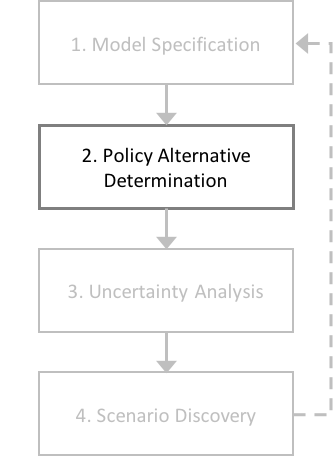
\includegraphics{structure-step2}
    \caption{RDM Structure - Step 2}
    \label{fig:structure-step2}
\end{figure}

\newpage

\section{Multi-Objective Evolutionary Algorithms (MOEAs)} \label{step2-moea}
Wicked problems characterized by tipping point behavior will generally involve multiple conflicting objectives due to their deeply uncertain nature. Because of this, there is no single optimal solution to these problems; instead, analysts must look for a set of potential alternatives, where each solution in the set is not dominated by any other solution in the set. This is known as Pareto optimality. To find the Pareto optimal set of solutions, analysis requires a search algorithm that is capable of handling conflicting objectives. The most common solution is what's known as a multi-objective evolutionary algorithm \citep{Maier2014, Reed2013}. A multi-objective evolutionary algorithm (MOEA) is one that takes a generic approach to optimization, where a population of potentially optimal items is generated through an iterative process of the following steps: 

\indent\textbf{Begin}: 
\begin{enumerate}[start=0]
    \item A set of options is randomly determined, the fitness of of which is determined based on the case-specific definition provided.
\end{enumerate}

\indent\textbf{Iterative Steps}: 
\begin{enumerate}[start=1]
    \item The most fit options are used to generate new options for consideration - the next generation of alternatives. 
    \item Fitness of those new options is determined using the same definition as in 0. 
    \item The options with the lowest fitness in the existing set are replaced with items of higher fitness in the newly discovered set. 
\end{enumerate}

Many MOEAs have been developed over the years, each of which aims to discover potential solutions to multi-objective problems. One of the earliest examples, NSGAII, is a generational algorithm that was developed by \citet{Deb2002}. A general MOEA replaces the entire population of currently tracked solutions after every search iteration \citep{Reed2013}. NSGAII uses a constant population size for each generation, and was one of the earliest to use Pareto dominance to search for and rank alternative solutions to a provided problem. 

After each search iteration, NSGAII uses a Pareto sorting algorithm to find the new population of non-dominated solutions when combining the existing set of solutions and the newly found population of potential alternatives. This results in a new set of non-dominated alternatives that is used in the next iteration \citep{Reed2013}. The goal of this search process is to find a set of non-dominated solutions that make up the Pareto optimal front, which would precisely describe the complex trade-offs between conflicting objectives. Due to the presence of uncertain behavior and conflicting objectives, however, it is impossible to reach the optimal front precisely. Therefore, the search process determines what is called an approximation of the Pareto front.  

To facilitate the search process, NSGAII makes use of a single operator that is responsible for maintaining diversity of solutions \citep{Reed2013, Ward2015}. The NSGAII algorithm has had solid performance in many optimization problems and is therefore still commonly used today \citep{Zheng2016}. 

The NSGAII algorithm was extended to create $\epsilon$-NSGAII by incorporating epsilon dominance in the sorting process and by using adaptive population sizing across the different generations. Together, these two characteristics have shown to reduce the need for extensive calibration of input parameters and to include more efficient search process \citep{Ward2015}. Epsilon dominance enables the decision maker to specify her desired level of precision for a policy to be considered dominant for each outcome of interest. With this property, solutions are only considered dominant if they fall outside the space defined by the epsilon value of an outcome of interest \citep{Horoba2008}. This allows for the elimination of alternatives that are considered similar and encourages diversity in the final set of recommended options \citep{Reed2013}. An epsilon value of 0 means that the Pareto sorting algorithm will behave similarly to one without any epsilon dominance considerations, as is found in traditional NSGAII. 

Along with epsilon dominance, adaptive population sizing allows for a more efficient search to be completed. The number of alternatives being tested can begin with a smaller population size to reduce computational cost. Once a more stable set of alternatives has been generated, the population size can be increased to put more pressure on the fitness and selection process, which ensures that the most fit solutions are being found in each generation \citep{Ward2015}. Other traditionally structured MOEA algorithms include SPEA2, $\epsilon$-MOEA, OMOPSO, MOEA/D, and GDE3 \citep{Reed2013, Ward2015, Zheng2016}. Each of these algorithms use a constant operator and some form of Pareto dominance to find solutions and maintain diversity.

An alternative to these traditional algorithms is a hybrid-MOEA known as Borg, which is built on the $\epsilon$-MOEA algorithm, a steady-state MOEA. Unlike a generational algorithm, a steady-state MOEA attempts to replace one solution in the existing set of alternative solutions after each search iteration, creating a highly efficient search process \citep{Ward2015}. 

Borg pairs the ideas of adaptive population sizing and epsilon dominance used in $\epsilon$-MOEA with a new auto-adaptive operator selection process and randomized algorithm restarts when search progress stalls to efficiently find well-performing solution alternatives \citep{HadkaReed2013}. By using auto-adaptive operator selection, as opposed to a single operator used as is used in earlier search algorithms, Borg is able to use operators based on their ability to select the strongest candidate solutions, leading to a more efficient and effective search process. The randomized restart function enables Borg, upon detecting that the search process has stalled, to inject new and diverse alternatives into the search process, ensuring the best chance for a diverse set of alternatives that more closely approximates the optimal Pareto front once the algorithm completes its run \citep{Reed2013}. 

Several studies have been completed that compare the success or failure of various MOEAs for a variety of policy problems. These studies have generally concluded that the auto-adaptive operator selection and adaptive population sizing together allow Borg to identify a more robust and diverse set of alternatives than other methods \citep{Reed2013, Ward2015, Zheng2016}. Algorithms apart from Borg that achieved at least some success are $\epsilon$-MOEA, NSGAII, and $\epsilon$-NSGAII, but none of these algorithms have provided results at the level of Borg. 

    \subsection{Auto-adaptive $\epsilon$-NSGAII} \label{hybridnsgaii}
    While Borg has been discovered to be quite successful at find a strong approximation of a problem's Pareto optimal front, it does so by leveraging a steady-state genetic algorithm. In this type of algorithm, only one new alternative is generated and folded into the existing non-dominated set at a time. This requires strategies to both select the desired parents from the existing set of alternatives and to prescriptively replace solutions in the existing set, both actions of which can significantly impact the outcome of the search process \citep{Vavak1996}, leading to the potential for additional uncertainty in analysis of a problem already fraught with uncertainty. Slow replacement of the non-dominated set can also contribute to slower convergence to the Pareto-optimal front \citep{Vavak1996}. 
    
    In contrast, a generational algorithm uses a much larger portion of the existing set of non-dominated solutions in each iteration of the search process to generate a new set of alternatives. These two sets are then compared to build an entirely new set of alternative solutions at the end of each iteration. This can lead to a faster convergence toward the Pareto optimal front \citep{Vavak1996}. 
    
    This research proposes an advancement of the traditional $\epsilon$-NSGAII algorithm that combines the strongest attributes of Borg: auto-adaptive operator selection and adaptive population sizing, with the best attributes of $\epsilon$-NSGAII: epsilon-dominance and a generational algorithm that has fast convergence to the Pareto optimal front. Instead of using a single operator as in the traditional $\epsilon$-NSGAII algorithm, auto-adaptive $\epsilon$-NSGAII uses a selection process similar to Borg to select an operator from the same group of operators that Borg considers. Each operator is assigned a probability of selection based on the number of solutions that an operator has produced that end up in the non-dominated set of alternatives after each search iteration. Operator elements and their parameter settings are indicated in \cref{table:nsgaii-hybrid}, and the complete operator definitions are listed below. 

    \begin{itemize}
        \item Simulated Binary Crossover (SBX) variator + Polynomial Mutation (PM) mutator
        \item Parent-centric Crossover (PCX) variator + PM mutator
        \item Differential Evolution (DE) variator + PM mutator
        \item Unimodal Normal Distribution Crossover (UNDX) variator + PM mutator
        \item Simplex Crossover (SPX) variator + PM mutator
        \item Uniform mutation (UM) mutator
    \end{itemize}

    \begin{table}[ht]
        \centering
        \captionsetup{width=0.57\textwidth}
        \caption[Auto-adaptive $\epsilon$-NSGAII configuration]{A sumary of the configuration details for the variant and mutator elements of the operators used in the proposed auto-adaptive NSGAII algorithm \citep{HadkaReed2013}}
        \label{table:nsgaii-hybrid}
        
        \setlength\arrayrulewidth{1pt}\arrayrulecolor{white}
        \rowcolors{2}{odd-row-blue}{even-row-blue}
        \begin{tabularx}{0.55\textwidth}{|l|X|r|}
            \rowcolor{tudelft-dark-blue!80}
            \color{white}\bfseries Name      &   \color{white}\bfseries Property Name   &   
            \multicolumn{1}{|l|}{\color{white}\bfseries Value} \\ \hline
            
                                   & probability            & $1.0 / L$        \\ \cline{2-3} 
            \multirow{-2}{*}{PM}   & distribution index     & $20$             \\ \hline
                                   & probability            & $1.0$            \\ \cline{2-3} 
            \multirow{-2}{*}{SBX}  & distribution index     & $15$             \\ \hline
                                   & nparents               & $3$              \\ \cline{2-3} 
                                   & noffspring             & $2$              \\ \cline{2-3} 
                                   & eta                    & $0.1$            \\ \cline{2-3} 
            \multirow{-4}{*}{PCX}  & Zeta                   & $0.1$            \\ \hline
                                   & crossover rate         & $0.1$            \\ \cline{2-3} 
            \multirow{-2}{*}{DE}   & step size              & $0.6$            \\ \hline
                                   & nparents               & $3$              \\ \cline{2-3} 
                                   & noffspring             & $2$              \\ \cline{2-3} 
                                   & zeta                   & $0.5$            \\ \cline{2-3} 
            \multirow{-4}{*}{UNDX} & eta                    & $0.35/\sqrt{L}$   \\ \hline
                                   & nparents               & $L+1$            \\ \cline{2-3} 
                                   & noffspring             & $L+1$            \\ \cline{2-3} 
            \multirow{-3}{*}{SPX}  & expansion              & $\sqrt{(L+1)+1}$  \\ \hline
            UM                     & probability            & $1.0/L$          \\
        \end{tabularx}
    \end{table}

    Alternative solutions are identified in the search process using tournament selection logic similar to what is found with the original $\epsilon$-NSGAII algorithm. As auto-adaptive $\epsilon$-NSGAII includes adaptive population sizing, the number of alternatives involved in each iteration of the tournament selection will change to match the size of the previously identified set of non-dominated alternative solutions. The initial population is determined using a Latin Hypercube sampling to build a set of alternatives based on the desired initial population size. A Latin Hypercube sampling ensures that each member of the decision lever set is represented evenly across the initial population \citep{Mckay1979}. In the case of this study, the initial population size will be 100. 
    
    The complexity of deeply uncertain problems and the large number of function executions needed mean that significant computing power is required for the MOEA to efficiently find as close an approximation to the Pareto front as possible. This can be accomplished through parallel computing. Borg, and other steady-state MOEAs can be parallelized through what is known as a master-slave architecture, in which a "master" process generates sub-problems that can run independently in their own processes. The results of these sub-problems are then returned to the master \citep{Zavoianu2013}. Such a scheme allows for a Borg-based search to make efficient use of CPU resources, as each sub-process is able to independently evaluate a single solution for potential replacement. However, there are limitations to the number of sub-processes that can be started at once to avoid  evaluating too many solution alternatives at the same time \citep{Hadka2013}. Furthermore, there is significant work required to develop a high-quality master-slave system to support parallelization of steady-state MOEAs \citep{Hadka2015Scale}. Parallelizing a generational algorithm like the proposed auto-adaptive NSGAII MOEA is much more straight forward, as each population member is independent from the others, with each iteration of the search process producing a new and independent population of alternatives with which to compare. Therefore, it is much simpler to take advantage of the computing power brought by parallelization for the proposed auto-adaptive $\epsilon$-NSGAII algorithm. A potential bottleneck does exist with a generational MOEA when the new population must be compared to the same existing set of non-dominated alternatives. Computational cost can be reduced here by using as efficient a Pareto sorting algorithm as possible. 
    
    The auto-adaptive $\epsilon$-NSGAII algorithm used for this study is implemented using the existing functions from the Python-based Platypus optimization package, which is a Python clone of the Java-based MOEAFramework. Platypus contains existing implementations of an epsilon-based search process, multi-operator management, tournament selection to determine potential solutions, and a Pareto-based sort to build the set of non-dominated solution alternatives. These pieces are combined to create the new auto-adaptive $\epsilon$-NSGAII algorithm. At the time of this thesis, Borg requires a paid license or special dispensation to use. Because the algorithm leverages existing open-source code, it is freely available for anyone to leverage in their own analysis. Details about where to find the implementation can be found in \cref{appendix-code}.

    \subsection{MOEA configuration}
    The auto-adaptive $\epsilon$-NSGAII algorithm is used for all three methods of robust decision support. Apart from the evaluation mechanism, which is discussed in \cref{step2-scenarios}, algorithm configuration is consistent across all methods under consideration to ensure a fair comparison by limiting the differences between methods as much as possible. Configuration is based on the parameters in \cref{table:moeaadditional}. This table also includes epsilon value settings, which were determined through referencing past research that has used the lake problem \citep{Quinn2017,Ward2015}, and by balancing the computational cost of having smaller epsilon values with the added benefit that smaller values may yield a closer approximation of the Pareto front. A study of the impact of different epsilon values on the search results for MORDM can be found in \cref{appendix-epsilon}. Traditionally, however, epsilon values are determined with input from the decision maker, who are able to indicate there preference for fine-grained control and computational efficiency. 

    \begin{table}[ht]
    \caption{Additional Configuration for the MOEA-based search}
    \label{table:moeaadditional}
    
    \setlength\arrayrulewidth{1pt}\arrayrulecolor{white}
    \rowcolors{2}{odd-row-blue}{even-row-blue}
    \begin{tabularx}{\textwidth}{|l|X|l|}
        \rowcolor{tudelft-dark-blue!80}
        \color{white}\bfseries Name          &
        \color{white}\bfseries Description   &
        \color{white}\bfseries Setting
        \\  \hline
        
        Population     & Starting number of policy alternatives that are tested each generation   & 100 \\ \hline
        
        \multicolumn{3}{|c|}{\cellcolor{tudelft-dark-blue!50}\color{white}Number Function Executions} \\ \hline
                                             & MORDM, multi-Scenario MORDM       & 500,000  \\ \cline{2-3} 
        \multirow{-2}{*}{Intertemporal}      & MORO                              & 300,000  \\ \hline
        Planned Adaptive DPS                 & All Methods                       & 100,000  \\ \hline
        DPS                                  & All Methods                       & 100,000  \\ \hline
        
        \multicolumn{3}{|c|}{\cellcolor{tudelft-dark-blue!50}{\color{white} Convergences}}  \\ \hline
        Epsilon Progress        & \multicolumn{2}{l|}{An indication of the search progress}           \\ \hline
        Operator Usage          & \multicolumn{2}{l|}{Usage of each operator as the search continues} \\ \hline
        \cellcolor{even-row-blue}    & MORDM                      & {[}2.5, 2, 1, 1{]}          \\ \cline{2-3} 
        \cellcolor{even-row-blue}    & Multi-Scenario MORDM       & {[}10, 2, 1, 1{]}           \\ \cline{2-3} 
        \multirow{-3}{*}{\cellcolor{even-row-blue}{ Hypervolume Limits}}  & MORO   & {[}1, 1, 1, 1{]} \\ \hline
        
        \multicolumn{3}{|c|}{\cellcolor{tudelft-dark-blue!50}{\color{white} Epsilon Settings}}  \\ \hline
        \multicolumn{2}{|l|}{Pollution Level}           & 0.1                                   \\ \hline
        \multicolumn{2}{|l|}{Utility}                   & 0.1                                   \\ \hline
        \multicolumn{2}{|l|}{Inertia}                   & 0.01                                  \\ \hline
        \multicolumn{2}{|l|}{Reliability}               & 0.01                                  \\
    \end{tabularx}
    \end{table}

    There are two small differences in configuration that are a part of \cref{table:moeaadditional}. Each of the problem iterations has its own setting for the number of function executions required for a single search to be completed. This number was established through testing of different values and was made large enough to ensure consistent convergence to a steady set of solution alternatives across independent search runs. The intertemporal variation of the lake problem requires a significantly larger number of function executions due to the much larger number of decision levers present in that variation (see \cref{step1-L} for details). The number of function executions configured for the intertemporal variation and MORO method pairing is lower than for the other two methods due to computational constraints, but consistent convergence was still achieved. 
    
    The second difference is in the hypervolume limits established for the convergence metrics. These values were established after testing of each robust decision support method and represent the approximate maximum values for each outcome of interest in the following order [pollution level, utility, inertia, reliability]. The hypervolume convergence metric does not affect the search process itself, but provides a mechanism for tracking stabilization of the search process. Hypervolume will be discussed further in \cref{results-convergence}. 

\section{Mechanism for Evaluation} \label{step2-scenarios}
The most critical element when configuring the search phase is the manner in which policies will be compared. Each of the RDM-based methods considered here have a different mechanism with which to accomplish this. MORDM and multi-scenario MORDM both use one reference scenario (at a time, in the case of multi-scenario MORDM) to test a policy against. The resulting values of the outcomes of interest are then used in the non-dominated selection process of the MOEA. In contrast, MORO test a policy against a set of scenarios and determines fitness by evaluating the robustness of the policy using the resulting sets of outcomes. These processes will be explained in more detail next. 

    \subsection{MORDM} \label{step2-mordm}
    MORDM is the earliest extension of the RDM method that introduced a formal mechanism to handle multiple conflicting objectives, through a multi-objective evolutionary algorithm-based search. Alternative policies that have been identified are compared in MORDM based on their performance in a single static reference scenario \citep{Kasprzyk2013}. That scenario is generally determined through conversation with decision makers, but in this case is based on the configuration used by \citep{Quinn2017}. Specific base values are found in \cref{table:uncertainties}. Policies are placed in the set of non-dominated options if they lead to stronger performance in that base scenario. This mechanism of evaluation, therefore, does not directly or indirectly incorporate robustness in the evaluation of alternatives. 

    \subsection{Multi-Scenario MORDM}
    As indicated in \cref{review-multi}, the fundamental difference between the MORDM and multi-Scenario MORDM methods is the repetition of the search process (as well as uncertainty analysis and scenario discovery) using more than one reference scenario. \cref{review-multi} discussed many potential ways to select the set of reference scenarios. This research uses a combination of two key techniques to select four scenarios that, when used in combination with the base reference scenario identified in \cref{step2-mordm}. The first is to leverage the uncertainty space that is revealed to cause vulnerabilities in policies found through the scenario discovery process in traditional MORDM, similar to the process discussed by \citet{Watson2017}. The second technique is to select a set of four maximally diverse scenarios from within a larger set of scenarios that fall within the identified vulnerable uncertainty space, as \citet{Eker2018} discussed. Specifically, this process involves steps listed below.
    
    \begin{enumerate}[leftmargin=*]
        \item Perform traditional MORDM-based analysis with a single reference scenario through the scenario discovery process. 
        \item Build a library of experiments that include uncertainty settings and how each set of uncertainty values respond under a group of different policies. This study examines how 500 sets of uncertainty values respond to a set of 10 different policies. These policies were determined by sampling across the lever space using a Latin Hypercube technique. The library of experiments will be used to select the four additional reference scenarios used in analysis. 
        \item Use the results of the scenario discovery process to select a subset of experiments with parameters that fall in the vulnerable ranges identified in scenario discovery. This subset of experiments will be used in the selection of four maximally diverse scenarios. 
        \item Given the subset of policy options, perform an exhaustive search of all possible combinations of four different policies to discover the maximally diverse set, based on the outcomes of interest. Diversity is determined in the same way as \citep{Eker2018}, who use euclidean distance between normalized values of the outcome indicators. Specifically, distance of a set of four policies is defined as in \cref{eq:step2-maxdistance} \citep{Carlsen2016}. The final set of policies selected is the one who has the largest calculated distance.
    \end{enumerate}
    
    \begin{equation}\label{eq:step2-maxdistance}
    distance = 1/2 * \underset{\forall j,k \in set}{min}{d_{k,j}} + 
               1/2 * \underset{\forall j,k \in set}{mean} {d_{k,j}}
    \end{equation}
    \begin{equation}\label{eq:step2-distancedef}
     d_{k,j} = \sqrt{\sum_{i} (\bar{o_{i,j}} - \bar{o_{i,k}})^{2}}
    \end{equation}

    The identified reference scenarios for each model variation are visualized in \cref{fig:selected-scenarios} and described in \cref{table:refscenario-inter,table:refscenario-adapt,table:refscenario-dps}. For all model variations, values are selected from the bottom half of the ranges for uncertainty parameters that relate to the removal of pollution from the lake, b and q, indicating that the policies discovered by the MORDM analysis tend to fail when the lake is not as successful at removing pollution on it's own. Values are selected from a a wide range for the other three uncertainty parameters. Also of note, the planned adaptive DPS variation revealed fewer uncertainty sets that resided in the vulnerable value ranges than the DPS or intertemporal variations, despite the selection being made from the same sized group of original scenarios as the DPS and intertemporal variations. It is unclear why that is at this point, whether it be that the model is more successful on it's own or that the MORDM process itself was more successful at discovering robust policies than the other two models. 
    
    Not included in this study is a comparison of different scenario selection techniques and the effect those techniques have on the results of analysis. The four selected scenarios are unique to each variation of the lake problem. These reference scenarios are then used to run the search process four separate times. This will result in four distinct sets of non-dominated strategies, each generated from a different reference scenario. 
    
    \begin{figure}[H]
        \centering
        \captionsetup{width=0.75\linewidth}
        
        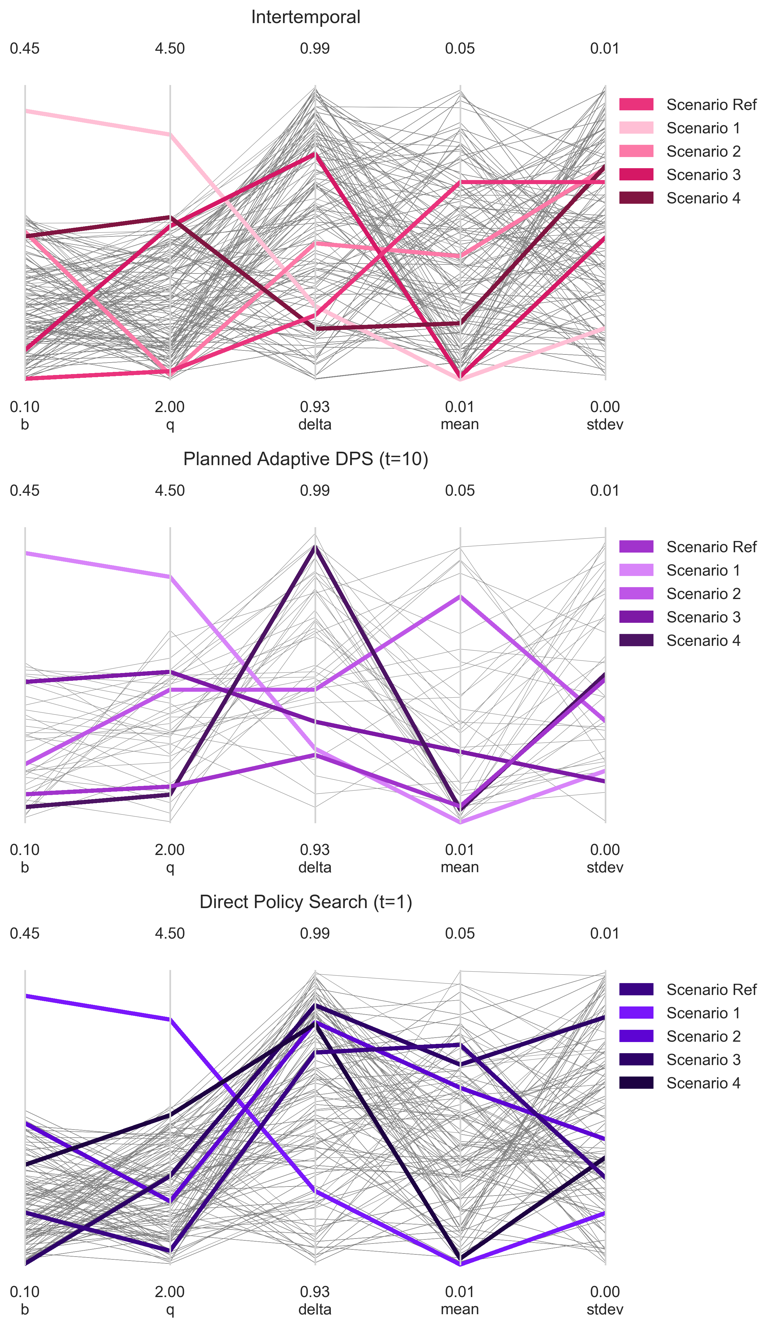
\includegraphics[width=0.75\linewidth]{scenarioselect/selected_scenarios}
        \caption[Uncertainty values used to select reference scenarios for multi-scenario MORDM]{Uncertainty values for the maximally diverse scenarios for each variation of the lake problem}
        \label{fig:selected-scenarios}
    \end{figure}
    
    \begin{table}[H]
        \centering
        \captionsetup{width=\textwidth}
        \caption[Reference Scenarios used for the intertemporal model variation]{Reference scenarios used for intertemporal analysis with the multi-Scenario MORDM method}
        \label{table:refscenario-inter}
        
        \setlength\arrayrulewidth{1pt}\arrayrulecolor{white}
        \rowcolors{2}{odd-row-blue}{even-row-blue}
        \begin{tabularx}{\textwidth}{|l|R|R|R|R|R|}
            \rowcolor{tudelft-dark-blue!80}
            {\color{white} Reference Scenario} & 
            \multicolumn{1}{|c|}{\color{white} b} & \multicolumn{1}{|c|}{\color{white} q} & \multicolumn{1}{|c|}{\color{white} mean} & \multicolumn{1}{|c|}{\color{white} stdev} & \multicolumn{1}{|c|}{\color{white} delta} \\ \hline
            
            1 & 0.2760 & 3.0490 & 0.0039 & 0.0039 & 0.9310 \\ \hline
            2 & 0.1350 & 2.0255 & 0.0407 & 0.0029 & 0.9613 \\ \hline
            3 & 0.2704 & 2.4783 & 0.0169 & 0.0039 & 0.9631 \\ \hline
            4 & 0.1009 & 3.6789 & 0.0187 & 0.0037 & 0.9317 \\ \hline
        \end{tabularx}
    \end{table}

    \begin{table}[H]
        \centering
        \captionsetup{width=\textwidth}
        \caption[Reference Scenarios used for the planned adaptive DPS model variation]{Reference scenarios used for planned adaptive DPS analysis with the multi-Scenario MORDM method}
        \label{table:refscenario-adapt}
        
        \setlength\arrayrulewidth{1pt}\arrayrulecolor{white}
        \rowcolors{2}{odd-row-blue}{even-row-blue}
        \begin{tabularx}{\textwidth}{|l|R|R|R|R|R|}
            \rowcolor{tudelft-dark-blue!80}
            {\color{white} Reference Scenario} & 
            \multicolumn{1}{|c|}{\color{white} b} & \multicolumn{1}{|c|}{\color{white} q} & \multicolumn{1}{|c|}{\color{white} mean} & \multicolumn{1}{|c|}{\color{white} stdev} & \multicolumn{1}{|c|}{\color{white} delta} \\ \hline
            
            1 & 0.1771 & 2.4274 & 0.0232 & 0.0048 & 0.9691 \\ \hline
            2 & 0.2084 & 3.3540 & 0.0399 & 0.0049 & 0.9872 \\ \hline
            3 & 0.3326 & 3.6983 & 0.0344 & 0.0040 & 0.9312 \\ \hline
            4 & 0.3939 & 4.0342 & 0.0257 & 0.0049 & 0.9522 \\ \hline
        \end{tabularx}
    \end{table}
    
    \begin{table}[H]
        \centering
        \captionsetup{width=\textwidth}
        \caption[Reference Scenarios used for the DPS model variation]{Reference scenarios used for DPS analysis with the multi-Scenario MORDM method}
        \label{table:refscenario-dps}
        
        \setlength\arrayrulewidth{1pt}\arrayrulecolor{white}
        \rowcolors{2}{odd-row-blue}{even-row-blue}
        \begin{tabularx}{\textwidth}{|l|R|R|R|R|R|}
            \rowcolor{tudelft-dark-blue!80}
            {\color{white} Reference Scenario} & 
            \multicolumn{1}{|c|}{\color{white} b} & \multicolumn{1}{|c|}{\color{white} q} & \multicolumn{1}{|c|}{\color{white} mean} & \multicolumn{1}{|c|}{\color{white} stdev} & \multicolumn{1}{|c|}{\color{white} delta} \\ \hline
            
            1 & 0.2683 & 3.5029 & 0.0430 & 0.0027 & 0.9429 \\ \hline
            2 & 0.1009 & 3.6998 & 0.0453 & 0.0044 & 0.9481 \\ \hline
            3 & 0.2187 & 2.0506 & 0.0428 & 0.0025 & 0.9504 \\ \hline
            4 & 0.1620 & 3.8685 & 0.0388 & 0.0022 & 0.9328 \\ \hline
        \end{tabularx}
    \end{table}

    \subsection{MORO}
    The MORO framework makes the most effort to incorporate considerations of robustness in the policy evaluation process, and does so in two steps. First, each alternative policy option is evaluated over a set of more than one scenarios; this study uses 50 scenarios for evaluation. Given the alternative's performance across those 50 scenario, policy alternatives are then used to calculate robustness values for each outcome of interest. These robustness values are then used to determine whether an alternative belongs to the set of non-dominated alternatives that the search process is building. The robustness definition in the search process is the same as is specified in \cref{step0-robust}, where a value between 0 and 1 is calculated that indicates the fraction of scenarios that meet the robustness threshold for each outcome of interest. By using robust values in the search process to determine the effectiveness of a potential policy alternative, it is more likely to build a set of alternatives that meet the robustness criteria that are targeted by decision makers. 

\section{Non-Dominated Selection of Alternatives} \label{step2-pareto}
Because there is an element of randomness to the MOEA's process, through the selection of the starting population of the search using a Latin Hypercube sampling across the decision lever space, this analysis will include multiple repetitions of each search in order to both study and manage the impact of the randomly selected starting population on the resulting set of non-dominated policy alternatives. Due to computational constraints, the number of variations changes depending on the method considered. Selected values are based on the computational requirements of that method and on the variation observed across searches. 

\begin{itemize}
    \item \textbf{MORDM}: 50 repetitions used
    \item \textbf{Multi-Scenario MORDM}: 20 repetitions per reference scenario used
    \item \textbf{MORO}: 10 repetitions used
\end{itemize}

Once the defined number of repetitions is complete, the resulting set of non-dominated policy alternatives is subjected to a final sort to build the ultimate set of non-dominated solutions. The algorithm used is also epsilon-based and uses the same configuration as the search algorithm \citep{Deb2002, Deb2005, Woodruff2013}. This final selection process results in a set of non-dominated policy alternatives that is not affected by the value of the random seed used. 
\chapter{Step 3: Uncertainty Analysis}\label{dev-step3}

\begin{abstract}
    Step 3 of an RDM-based analysis examines the performance of the set of non-dominated policy alternatives discovered during the policy alternative determination step across a large set of potential future states of the world (SOWs). This step is common for all three methods under consideration, with the only difference being that uncertainty analysis is repeated for each reference scenario used in multi-scenario MORDM. The first element of uncertainty analysis, computational exploration, is described in \cref{step3-explore}. In addition to exploring how each policy alternative responds to a variety of potential SOWs, the uncertainty analysis phase includes calculating the robustness of each policy based on the results of that exploration, which is discussed in \cref{step3-robust}.
\end{abstract}

\medskip

\begin{figure}[h]
    \centering
    \captionsetup{justification=centering}
    
    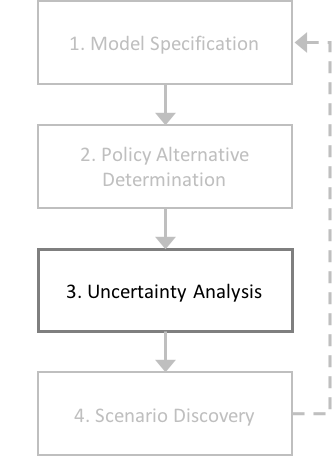
\includegraphics{structure-step3}
    \caption{RDM Structure - Step 3}
    \label{fig:structure-step3}
\end{figure}

\newpage

\section{Computational Exploration}\label{step3-explore}
The first part of uncertainty analysis, computational exploration, involves examining how each policy in the non-dominated set of alternatives behaves under an large ensemble of potential future states of the world. Remember that these alternatives were selected based on their performance in one, in the case of MORDM and multi-scenario MORDM, or only 50, in the case of MORO, scenarios. Computational experimentation, then, reveals how the identified alternatives behave given a much broader ensemble of potential future SOWs \citep{Kasprzyk2013}. 

The first part of computational exploration is to build a large ensemble of uncertainty vectors, accomplished through sampling across the uncertainty space identified in model specification. Several sampling strategies are available to build the ensemble of SOWs, including random sampling, importance sampling, and Latin Hypercube Sampling (LHS). This study makes use of LHS, as it provides an efficient way to divide the uncertainty space evenly with even a small sample size \citep{Helton2006}. The LHS technique ensures, that the entire range of each uncertainty parameter is equally represented in the sample set, which guarantees that no one uncertainty parameter is weighted more significantly in the exploration \citep{Mckay1979}. LHS is, therefore, ideal in cases involving a computationally expensive model as it can build an ensemble that describes the entire uncertainty space in with fewer scenarios than would be required with a purely random technique. 

The uncertainty space is defined in \cref{table:uncertainties}, and is sampled to build an ensemble fo 10,000 vectors of the five uncertainty parameters. Each policy from the non-dominated set of alternatives is tested against the generated ensemble of uncertainty vectors. This results in a large data set that describe how each policy behaves across the uncertainty space. That information is used in the next key part of uncertainty analysis, calculation of policy robustness. 

As a note, the individual sets of non-dominated policy alternatives generated in the second step of multi-scenario MORDM are evaluated separately for computational exploration, and result in separate results. 

\section{Robustness Calculation}\label{step3-robust}
Now that there is a large data set that describes each policy's performance across a broad set of potential future SOWs, robustness of each policy can be calculated. At this stage, the policy analyst selects their desired robust metric, or can select more than one metric, which may reveal different features of a policy's robustness. That decision, along with the exact configuration of the selected robust metric(s), should be made in conversation with decision makers, to ensure that their preferences and goals are accounted for \citep{Kasprzyk2013}. 

In this study, one robust metric is used: domain criterion satisficing. The exact implementation and configuration of this metric is specified in \cref{step0-robust}. Fundamentally, though, domain criterion satisficing involves determining the fraction of total scenarios for which a policy achieves the specific threshold for each outcome of interest. Each outcome of interest will have a separate robustness value, making it easier to communicate conflicts and trade-offs among the outcomes.

\chapter{Step 4: Scenario Discovery}\label{dev-step4}

\begin{abstract}
    The final piece in any RDM-based analysis is scenario discovery, which explores the data generated during uncertainty analysis to discover vulnerabilities that one or more of the identified policy alternatives does not address. This chapter will elaborate on the theory of scenario discovery in \cref{step4-scenariodiscovery} and will then detail the implementation used in this study \cref{step4-implementation}. 
\end{abstract}

\medskip

\begin{figure}[h]
    \centering
    \captionsetup{justification=centering}
    
    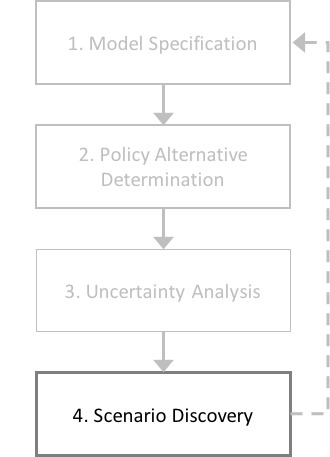
\includegraphics{structure-step4}
    \caption{RDM Structure - Step 4}
    \label{fig:structure-step4}
\end{figure}

\newpage

\section{Scenario Discovery Theory} \label{step4-scenariodiscovery}
The fundamental goal of scenario discovery is to determine which characteristics of a problem, including uncertainty and policy lever settings, lead to specific outcome behaviors \citep{Bryant2010}. When only a small number of scenarios are being considered at a time, it is easier to see patterns and determine which elements of those scenarios lead to a specific outcome behavior without further processing or cleaning. However, given the rise of computer-aided experimentation, the number of scenarios and policies considered can increase dramatically \citep{Lempert2008}. In the case of an RDM-based analysis, 10,000 or more scenarios can be considered, along with tens or even hundreds of policy options. This makes it impossible to detect patterns that affect system behavior. 

Scenario discovery within an RDM-based method aims to develop easy to understand descriptions of which areas of the uncertainty space remain vulnerable, despite searching for policy alternatives that are meant to be the most successful \citep{Kasprzyk2013}. This typically involves statistical and data-mining algorithms to discover patterns in a set of data. The two most commonly recognized scenario discovery algorithms are CART, a classification algorithm, and PRIM, a bump-hunting algorithm \citep{Lempert2008}. Research that has compared the two algorithms has discovered that while both PRIM and CART generally result in similar information, PRIM provides more opportunity for interaction and requires less initial configuration for the analyst \citep{Bryant2010}. Because of this, PRIM will be used for this analysis. 

\subsection{Patient rule induction method (PRIM)}
PRIM, also known as the Patient Rule Induction Method, uses a bump-hunting algorithm to identify a range of values that best predict the behavior of a subset of cases from the entire data set that fail to meet a specific goal \citep{Friedman1999}. To accomplish this, PRIM optimizes along three different axes: density, coverage, and interpretability, and attempts to maintain an even balance between density and coverage. Density refers to the fraction of cases in an identified cluster in which failure is recognized; coverage concerns the fraction of identified failure cases that are contained within that cluster; interpretability incorporates the ease with which users are able to understand what is discovered by the algorithm \citep{Lempert2013}. 

The algorithm involves initial configuration, followed by a series of two iterative and interactive steps that search for any common elements that correspond to a specific behavior of interest. 

\begin{enumerate}[leftmargin=*]
    \item Determine which experiments are of interest. This generally involves a classification mechanism in which experiments that lead to one or more outcomes of interest which doesn't meet a specific threshold. This can be, for example, the robustness thresholds specified in the configuration of the domain criterion metric in \cref{step0-robust}. 
    \item Search for regions
    \begin{enumerate}
        \item The algorithm constructs a series of boxes that are increasingly smaller and denser by slowly restricting the input space based on the removal of a small subset of elements that will lead to the greatest increase of the mean inside that new box. This step concludes with a series of boxes known as a "peeling trajectory" \citep{Lempert2008}
        \item The peeling trajectory is presented to the analyst, who is able to select one or more of the boxes that most effectively balances goals of having high density and high coverage \citep{Lempert2008}. These boxes are known as candidate boxes. Candidate boxes describe the ranges of various input parameters (whether that be uncertainties, decision levers, or both) that describe the behavior found in each box. 
        \item The analyst is able to restart the process to construct a new series of boxes. The algorithm will remove all data sets that are included in the first series and start again. The process can repeat until the analyst has discovered all useful information and ends the search. 
    \end{enumerate}
\end{enumerate}

%TODO describe this algorithm in more detail, including sample peeling trajectories....?

\section{Implementation Details} \label{step4-implementation}
PRIM has been implemented as an open-source algorithm using many different languages, including R and Python, making it easy to use; this analysis specifically will leverage the Python-based implementation found in the EMA-Workbench \citep{Kwakkel2016SD}.

This implementation of PRIM for this study involves developing a binary classification of the cases of interest, where 1 indicates that case should be considered by the PRIM algorithm, and a 0 means it does not include the behavior of interest and should therefore be ignored. Case classification will consider each outcome separately by selecting cases that do not meet the robustness threshold as defined in \cref{step0-robust} for each outcome of interest. Analysis will consider uncertainties and decision levers as drivers of behavior both separately and together.

Again, scenario discovery is executed for each set of non-dominated policy alternatives. This means that during multi-scenario MORDM, the scenario discovery process is run independently for each selected reference scenario. 

\chapter{Methods of Comparisons}
\label{dev-comparisons}

\begin{abstract}
    This chapter establishes framework for comparing robust decision support methods. This includes several points of comparison, both qualitative and quantitative. Measures will be grouped into categories that indicate the type of information being compared. This includes elements related to the setup and configuration process (\cref{compare-setup}), communication of the strength of results communication (\cref{compare-communication}), and comparisons of the results themselves (\cref{compare-results}).
\end{abstract}

\newpage

\section{Metric Selection Process}\label{compare-intro}
The metrics for comparison described in this chapter will provide a comprehensive look at the relative strengths and weaknesses of each problem variation and robust decision support method pairing. The metrics were developed based on a detailed review of existing work that compare various methods of decision support. As discussed in \cref{gap-comaprativework} and \cref{gap-policies}, previous literature has primarily focused on a comparison of two methods of decision support at a time for a single and specific problem variation \citep{Gersonius2016,Hall2012,Kwakkel2016Compare,Matrosov2013a,Matrosov2013b,Roach2015,Roach2016}. That literature has focused on points of comparison specific to the problem and methods under consideration at the time. The goal of this comparison framework is to build a library of comparison metrics that will facilitate a comprehensive comparison of multiple problem variations and multiple methods of decision support. 

\section{Setup Complexity} \label{compare-setup}
The first set of measures relates to the complexity of setup and use of each method. These are both qualitative measures that are related to each method and are independent of the problem variation under consideration. 

\begin{enumerate}[leftmargin=*,align=left,label=\textbf{Comparison \arabic* :}]
    \item Complexity of problem setup \newline
          Based on earlier work comparing methods of decision making, this metric draws attention to the effort required to prepare the problem under consideration for analysis \citep{Kwakkel2016Compare,Roach2015}. This metric considers the following: what elements must be specified before execution and how the model must format uncertainties, decision levers, and outcomes of interest. The end result will be an inventory of the model-specific configuration which focuses on elements that are unique to each method. 
    \item Complexity of method setup \newline
          This metric considers any method-specific setup that is required for the decision support method to be executed. Similar to metrics used in comparative research completed previously, complexity of method setup considers the availability of tools and software packages required to execute each method \citep{Gersonius2016, Kwakkel2016Compare}. Under this metric, the amount of work (through additional code and analysis beyond what is provided directly by any available tools), will be considered. The end result will be an inventory of the method-specific configuration which focuses on elements that are unique to each method.
\suspend{enumerate}

\section{Communication}\label{compare-communication}
Both quantitative and qualitative, these metrics describe the strength of method and results communication. 

\begin{enumerate}[resume,leftmargin=*,align=left,label=\textbf{Comparison \arabic* :}]
    \item Results communication \newline
          This metric refers to whether methods communicate results throughout execution or only upon completion of the entire analysis. This metric will examine differences in the recommended policy set if it is reported progressively. Also considered is the type of information that is communicated at different points during the analysis apart from the set of recommended policies. 
          
    \item Robustness communication \newline
          This metric, specific to the robustness metric used in the execution of each method, indicates whether the robustness metric is an abstract or direct representation of policy measures. Similar measures have been used in the past to indicate the ability of a method to effectively recommend robust policy solutions \citep{Gersonius2016, Roach2015}.

    \item Ease of results updating if the model specification changes \newline
          Wicked problems with tipping point logic are characterized by deep uncertainty, so the models that describe these problems can never be exact. These models are subject to frequent changes based on new data or additional input from decision makers, whether it be to uncertainty ranges, model structure, or policy levers. Therefore, it is important to consider how decision support methods respond to these changes \citep{Gersonius2016}. This metric examines how each method is able to respond to changes in the model under analysis by describing the way in which a change to the model specification can be incorporated in each of the three steps following specification for each method. Then, that information is compared to discover the elements that are unique to a specific method, which reveals how easily a model specification change can be reflected in analysis.

    \item Ease of results updating if desired robustness measure changes \newline
          As discussed in \cref{review-robustness}, the selected robustness measure has a significant impact on the recommendations made by each decision support method. A change in robustness measure may occur due to changing interests of the decision maker, or a desire to consider multiple robustness perspectives for the same problem. This metric supports the previous by indicating the ability for each method to quickly and easily respond to a change in robustness measure. 
\end{enumerate}

\section{Results}\label{compare-results}
The final set of metrics are quantitative in nature and focus on comparing the resulting recommended policy sets for each method and problem variation pairing. 

\begin{enumerate}[resume,leftmargin=*,align=left,label=\textbf{Comparison \arabic* :}]
    \item Computational cost \label{compare-computationcost} \newline
          Computation cost will be measured in the number of model executions required for both the policy alternative determination and uncertainty analysis steps. This is also known as the number of function executions.

    \item Convergence of search \newline
          This metric examines the impact of each method on the convergence of the MOEA-based search to a stable set of non-dominated policy alternatives in the policy alternative determination step. Examining the impact of different MOEA searches on the ability to reach a stable result will provide guidance on the necessary number of function executions required for future analyses.

    \item Robustness of recommended policy sets \label{compare-robustness} \newline
          When methods use similar robustness measures to evaluate policy options, as is the case for the methods considered in this study (see \cref{step0-robust}), this metric examines the differences in robustness calculated for each set of recommended solutions by comparing the mean, minimum, and maximum robustness values for each outcome of interest per model variation and method pairing.
    
    \item Similarity of recommended policy sets \newline
          Once final sets of policy alternatives are determined for each pairing, this metric compares the similarity of policy options in each set. This provides a mechanism for determining whether each pairing reaches similar insights independent of the robustness calculation for each policy in the final set \citep{Hall2012}. \Cref{compare-policysimilarity} describes the mechanism used to determine similarity for this and other comparison methods described. Given that measure, overall similarity of policy sets will be determined by comparing the mean of all measures for a pairing. The 10\textsuperscript{th} and 90\textsuperscript{th} percentile values will be compared, which should provide an idea of the level of similarity between two sets of policy alternatives. Because this metric involves comparing policy lever values, comparisons will be made within a specific variation of the problem under consideration.

    \item Similarity of robustness \newline
          For cases where methods use the same robustness measure but involve different procedures to calculate robustness for identified policy alternatives. This metric compares the robustness value of policies that are considered similar (based on the similarity mechanism defined in \cref{compare-policysimilarity} and the policy alternatives that fall in the 10\textsuperscript{th} percentile of similarity values). This communication, paired with the analysis of overall robustness of recommended policy sets (see \hyperref[compare-robustness]{\textit{Comparison 9}}), provides an guideline for how selection of a specific method may affect final robustness values. For example, this may indicate that one method leads to lower robustness values, despite similar policies being recommended. Given that the robustness values, like the policy values, are a vector of multiple distinct values, a mechanism must be defined to determine similarity. A description of this mechanism can be found in \cref{compare-policysimilarity}. 
\end{enumerate}

\section{Determining Similarity} \label{compare-policysimilarity}
Each recommended policy is represented as a vector of values. Therefore, similarity must be determined through a clearly defined distance measure. The selection of similarity measure will have a large impact on the comparisons made in this study, as it will be used in more than one of the comparison metrics defined in \crefrange{compare-setup}{compare-results}. 

In the case of the problems under consideration, policy and robustness data are both quantitative and dimensionless vectors. Based on two studies that compare several similarity and dissimilarity metrics, both qualitatively and quantitatively, the similarity measure identified as the most appropriate for this research is Euclidean distance \cite{Buttigieg2014, Shirkhorshidi2015}. Euclidean distance is one of the most well-known methods for determining the distance of numerical data sets \citep{Shirkhorshidi2015} and is most appropriate when considering quantitative value sets of homogeneous data \citep{Buttigieg2014}, which is what is found in both the policy and robustness vectors. 

Euclidean distance has a few recognized disadvantages, each of which is addressed and mitigated in this study. First, that it may indicate two vectors of distinct values are closer together than another pair of vectors that share one or more common values \citep{Shirkhorshidi2015}. Similarity comparisons in this research involve continuous data. Because of this, vectors sharing common values are not necessarily more similar if other values have larger differences. For example, the vectors <0.05, 0.20, 0.34> and <0.05, 0.015, 0.34>, with two common values, should not be considered as more similar than vectors <0.05, 0.20, 0.34> and <0.04, 0.21, 0.33>, with no common values. Therefore, this first disadvantage will not negatively affect the similarity calculations in this research. 

Related to the how difference in values of a vector element should be perceived when determining the similarity of two policies is the potential impact that a small change in value of a decision lever may have on the developed model. Due to the fact that the lake problem includes non-linear behavior characteristics, even a small change in a decision lever can lead to a significant impact to the system. A Euclidean distance calculation may indicate that two policies are quite similar, but those same two policies may yield significantly different results due to the presence of that non-linear behavior. A calculation of the similarity of policy vectors, therefore, indicates only that the policies themselves are similar and does not indicate anything about the similarity of the outcomes of the system when these policies are applied. 

Second, Euclidean distance can be dominated by the element with the largest potential value. Therefore, values should be normalized when vectors include members of different scales \citep{Shirkhorshidi2015}. Based on the defined mechanism for determining robustness (see \cref{step0-robust}), the robustness vector contains values of the same scale and do not need to be normalized. However, the policy vector is defined with variables that have varying ranges of possible values. Therefore, policy similarity will be determined using normalized policy vectors. 

Finally, Euclidean distance is strongly impacted by the size of the vectors being considered. Vectors that have many elements will often have larger distance values than vectors with a smaller number of values. As \cref{eq:euclid} shows, Euclidean distance is based on a summation of matching terms of the two vectors, represented by X and Y. 

\begin{equation} \label{eq:euclid}
distance(X, Y) = \sqrt{ \sum_{i=1}^{n}(x_i - y_i)^n}
\end{equation}

It is vital to be aware this property of a Euclidean distance calculation when comparing distance values to one another. A distance value of a pair of vectors with 4 elements can be smaller than a value calculated from a pair of vectors with 100 elements, for example, simply due to the significantly larger number of terms involved in the latter case. This study addresses this issue by ensuring that distance values are compared to each other only when calculated for vectors of the same length. For example, a distance calculation over vectors of decision levers for the intertemporal and DPS problem variations will never be directly compared to each other, because the DPS variation has only 5 elements, while the intertemporal variation has 100 elements.  

To contrast, an alternative and also commonly used distance measure is the Mahalanobis distance. Unlike Euclidean distance, which treats each element of a vector as independent and equally weighted, the Mahalanobis distance calculation uses the covariance matrix of the two vectors to account for an correlation that exists between two elements. The correlation matrix is represented by $S$ in \cref{eq:mahalanobis}, the equation for calculating Mahalanobis distance of two vectors, X and Y. Using the covariance matrix also means that there are no issues relating to the scale of different elements in a vector. However, as the three measures described previously reduce the impact of the recognized weaknesses of a Euclidean distance calculation, and because the Euclidean distance is much simpler to calculate, it will be used in this study instead of the Mahalanobis distance. 

\begin{equation} \label{eq:mahalanobis}
distance(X, Y) = \sqrt{ (X - Y)S^-1(X-Y)^T }
\end{equation}

Euclidean distance will be calculated practically with the Python-based SciPy library and using the method \texttt{scipy.spatial.distance.euclidean}. This method will accept two normalized policy vectors and will return the Euclidean distance. In \cref{eq:euclid}, the two normalized policy vectors are represented by X and Y. 

Each policy and robustness vector will be compared with every other vector, which results in a two-dimensional matrix of Euclidean distance values. The following holds true for distances in this matrix: $distance(X,Y) == distance(Y,X)$, so the resulting matrix will be bisymmetric, where the upper triangle will be equal to the lower triangle, separated by a diagonal of zeros. Because of this, an upper triangular matrix will be constructed where the lower triangular values are set to zero, which will be further processed in the targeted comparison method. 


\part{Results} \label{part-analysis}
\label{analysis-results}
\chapter{Initial Results} 

\begin{abstract}
This chapter will present individual results of each of the model+method pairings without any direct comparisons made. Each pairing combines one model variation with one decision support method, both based on the configurations developed in \cref{part-develop}. The individual results provide a foundation for the comparisons made next, in \cref{chapter-comparison}. Results will be presented in three stages: policy alternative determination in \cref{results-step2}, uncertainty analysis in \cref{results-step3}, and finally scenario discovery in \cref{results-step4}. As the model specification phase does not include any direct results apart from the development of models that are used in the remaining steps, and as the model variations do not change based on the method used, there is no specific section that covers that step in this chapter. For details on the implementation of each model variation, see \cref{dev-step1}. 
\end{abstract}

\newpage

\section{Step 2: Policy Alternative Determination} \label{results-step2}
Given a model, the next step of the analysis for each of the three methods under consideration is to search for a set of non-dominated policy alternatives. This section examines the outcome of that search, including convergence behavior and the resulting set of non-dominated alternatives. 

    \subsection{Convergence of the search process} \label{results-convergence}
    The search process used in this analysis included several convergence metrics, which are used to track the progress and stabilization of the search process. This section will discuss the results of two of the most commonly used metrics: epsilon progress and hypervolume convergence \citep{Reed2013,Ward2015}. Epsilon progress indicates whether new policies are being added to the set of non-dominated alternatives as the search progresses \citep{Ward2015}. Of interest for this metric is the slope of the epsilon progress line. A flat slope means that few or no new policies are being added to the set of non-dominated alternatives, indicating that the search process is no longer finding new alternatives. The goal of an MOEA-based search in the context of epsilon progress is to use enough functional executions to reach the point when the slope flattens out.
    
    Hypervolume provides a picture of the possible objective space that is being covered by a set of policy alternatives, given the boundaries of the space that is provided to the search algorithm \citep{Reed2013}.  See \cref{table:moeaadditional} for the hypervolume settings used in this analysis. Again, of interest is the slope of hypervolume curves. A flatter slope indicates that, even if new policies are being added to the set of non-dominated alternatives, those policies are not contributing to the diversity of the set of non-dominated alternatives. Therefore, those new additions do not reveal any significantly new information about potentially successful combinations of decision lever settings.
    
    Both of these metrics are plotted for every model+method pairing. Given that multiple independent repetitions were performed for each model+method search in order to reduce the impact of randomness that exists in the MOEA, one curve in a plot corresponds to one search repetition. In addition to the two plots that show the epsilon progress and hypervolume as the number of function executions builds, there is a plot of the relationship between hypervolume and epsilon progress. Of interest here is a positive correlation between hypervolume and epsilon progress, indicating that as the search adds new alternatives to the non-dominated set, it also increases the diversity of that set. A flat, horizontal slope here indicates that even though new alternatives are being added to the set of non-dominated policies, those new alternatives are not contributing to the diversity of the set. This is another indication of the stabilization of the search process. For a discussion of the other convergence metrics that were configured, which track the use of each of the five operators in the auto-adaptive NSGAII algorithm, see \cref{appendix-operatorconvergence}.
    
    As a note, the convergence metrics for all five reference scenarios of multi-scenario MORDM are plotted on the same chart. The reference scenarios each display different convergence trends. For example, the hypervolume and maximum epsilon progress of the non-dominated sets of policy alternatives found using each reference scenario converge to different values. The difference in values with respect to stabilization is important to keep in mind as the convergence plots for multi-scenario MORDM are presented.
    
        \subsubsection{Intertemporal}
        Due to computational and memory constraints, the number of functional executions for the intertemporal lake model changes per method. For both MORDM and multi-scenario MORDM, 500,000 functional executions are used. For the MORO method, 300,000 functional executions are used. \cref{fig:convergences-inter-planned} contains the convergence visualization for each method.
        
        In general, these plots show that the MOEA search is able to reach a stable epsilon progress and hypervolume, with quite consistent results for MORDM-based analysis. The MORO convergence plots do indicate a fairly significant early difference in the hypervolume, but that this value trends toward a much more similar final hypervolume (save one exception).

        \begin{figure}[H]
            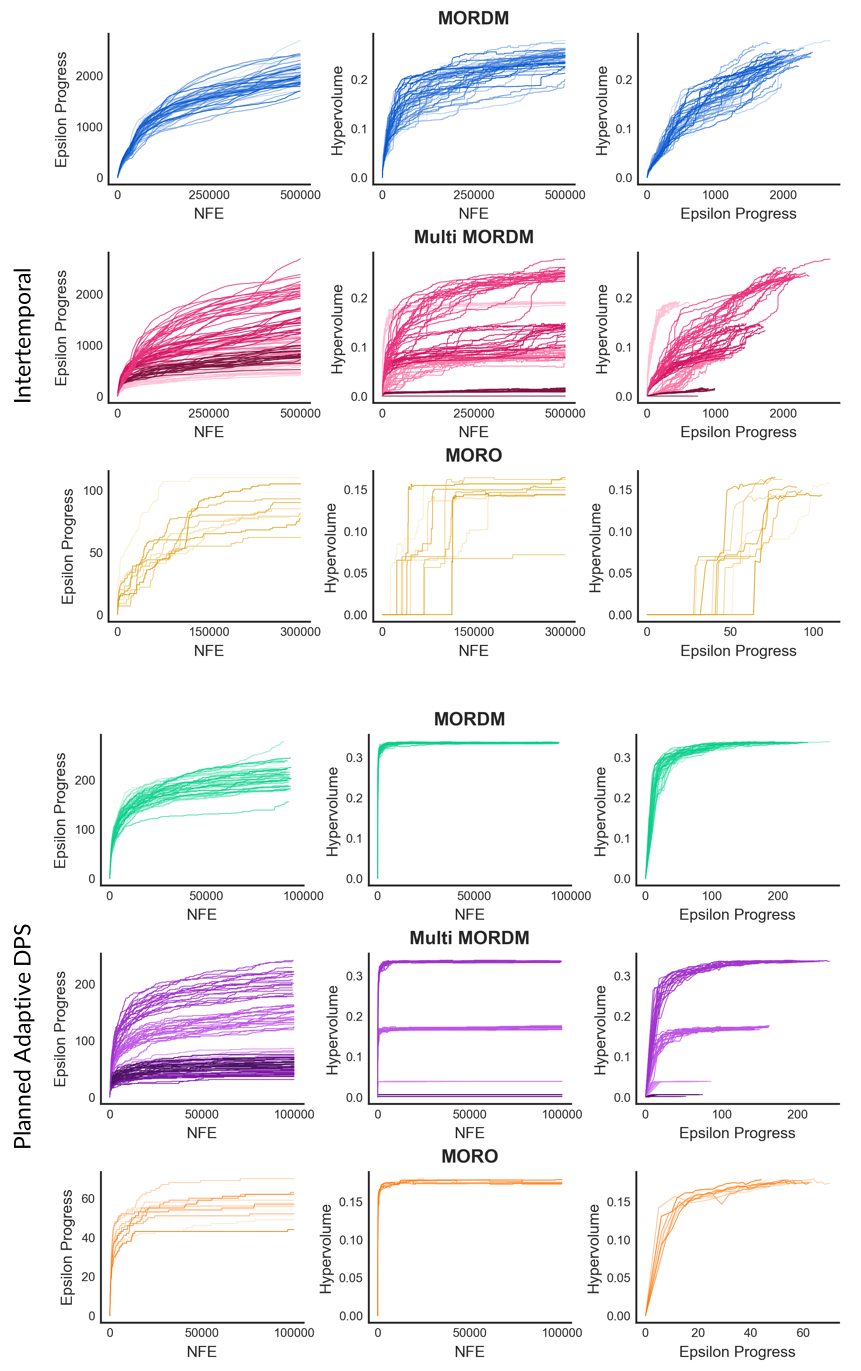
\includegraphics[height=\dimexpr
            \textheight-2\baselineskip-\abovecaptionskip-\belowcaptionskip\relax]{convergences/convergences_inter_planned}
            \caption[Convergences for the intertemporal and planned adaptive DPS variations]{Intertemporal and Planned Adaptive DPS convergences for each method. The first two plots in each row show the the relationships between epsilon progress, hypervolume, and number of function executions (NFE). The third shows the relationship between hypervolume and epsilon progress.}
            \label{fig:convergences-inter-planned}
        \end{figure}
        
        \begin{figure}[H]
            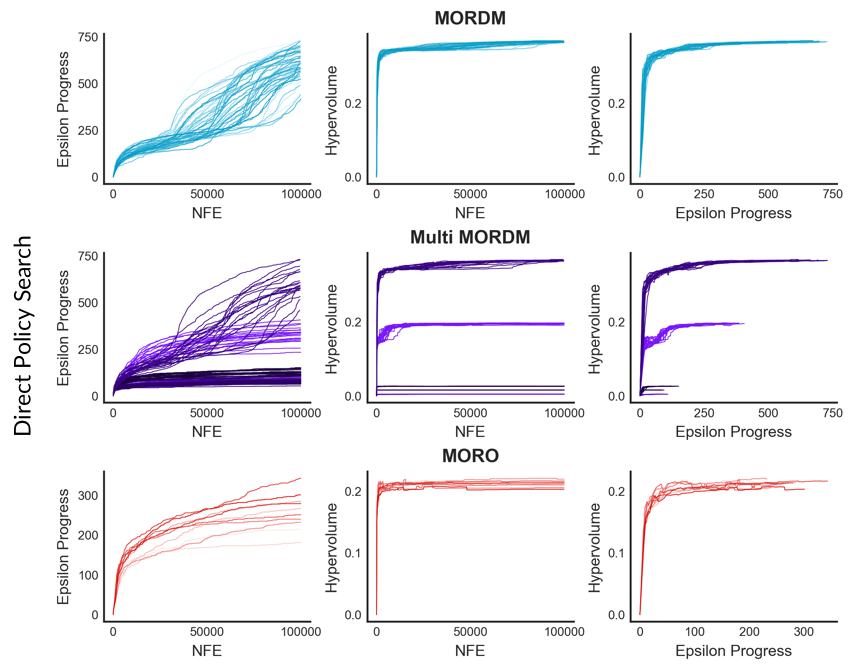
\includegraphics[width=\textwidth]{convergences/convergences_dps}
            \caption[Convergences for the DPS variation]{DPS convergences for each method. The first two plots in each row show the the relationships between epsilon progress, hypervolume, and NFE. The third shows the relationship between hypervolume and epsilon progress.}
            \label{fig:convergences-dps}
        \end{figure}

        As noted, the multi-scenario MORDM convergences for the intertemporal problem variation include convergences to different maximum epsilon progress values and hypervolumes. Despite the differences in maximum values seen between the different reference scenarios, each scenario independently reaches stabilization. 

        \subsubsection{Planned adaptive DPS}
        The planned adaptive lake problem used 100,000 function executions in each method's search phase to build non-dominated sets of policy alternatives. The search processes built convergences that are plotted in \cref{fig:convergences-inter-planned}, where each curve represents one repetition of the search process. 
        
        Across all methods, these plots indicate rapid and fairly consistent convergence to a stable hypervolume. Additionally and similar to the intertemporal problem, each reference scenario in multi-scenario MORDM analysis yield different but rapidly converging hypervolumes. Epsilon progress also levels off quite quickly for all methods, and there is a consistent and stable correlation between hypervolume and epsilon progress. All of these pieces of information, together, indicate a consistently successful search process, in terms of convergence. Furthermore, similar behavior is seen for the multi-scenario MORDM method in the case of planned adaptive DPS as was described for the intertemporal problem variation. Though each reference scenario stabilizes at a different value for hypervolume and epsilon progress, stabilization still occurs at a similar rate and by the final function execution of the search process. 

        \subsubsection{DPS}
        The DPS lake problem also used 100,000 function executions in each method's search process to build non-dominated sets of policy alternatives. The search processes built convergences that are plotted in \cref{fig:convergences-dps}, where each curve represents one repetition of the search process. 
        
        The hypervolume values of each method converge quite quickly to a small range of values. Epsilon progress also flattened out as the search process continued in the MORO and for most reference scenarios in the multi-scenario MORDM methods. The MORDM search process, using the base reference scenario specified in \cref{table:uncertainties} and which corresponds to the reference scenario in the multi-scenario MORDM plots with similar behavior, indicates both flat stretches and significant increases in epsilon progress throughout the search process, depending on the repetition. However, when the hypervolume convergence and relationship between epsilon progress and hypervolume are considered along with isolated epsilon progress, the changes in epsilon progress do not seem to add diversity to the non-dominated set of policy alternatives after the very early stages of search. This indicates that an NFE of 100,000 is sufficient to determine as diverse a set of non-dominated policy alternatives as possible. 
        
        Finally and similar to the intertemporal and planned adaptive DPS variations, the plots for multi-scenario MORDM for the DPS variation indicate that each reference scenario converges to a different hypervolume and epsilon progress. However, each reference scenario is still able to reach stabilization. 
        
    \begin{table}[ht]
        \centering
        \caption[Size of non-dominated policy alternative sets]{Size of the final non-dominated set of policy alternatives for each method and variation of the lake problem}
        \label{table:paretosize}
        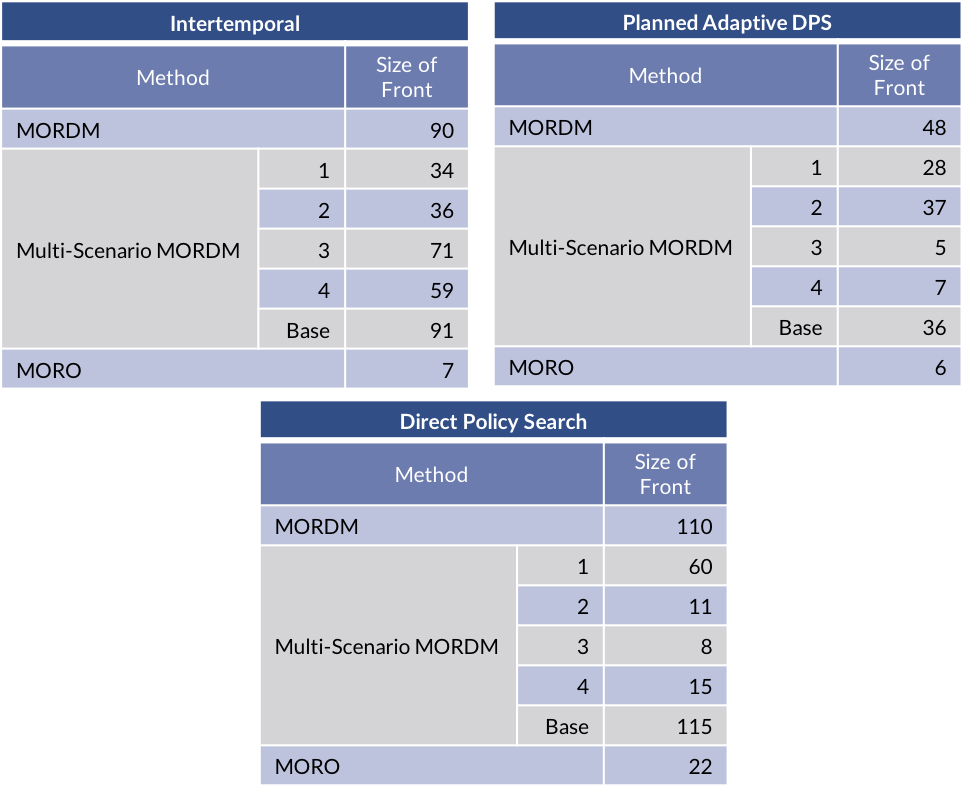
\includegraphics[width=\textwidth]{convergences/pareto_front}
    \end{table}
    
    \begin{figure}[ht]
        \centering
        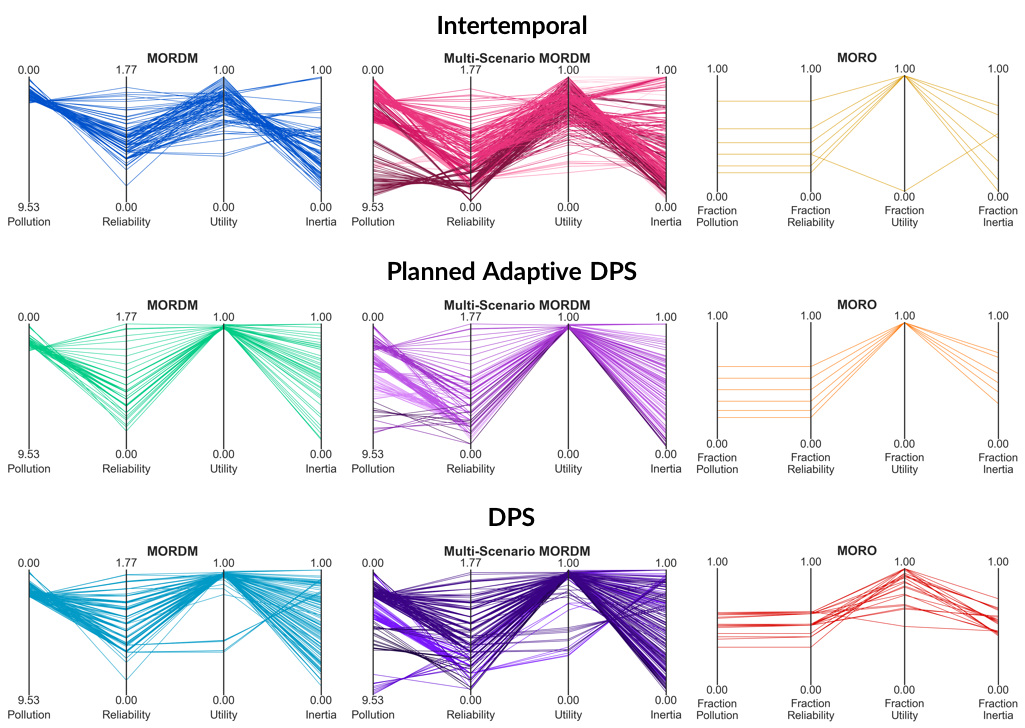
\includegraphics[width=\textwidth]{convergences/nondominated_outcomes_all}
        \caption[Outcome value ranges across all pairings]{Ranges of outcome values for each member of the non-dominated set of policy alternatives. The desirable values for each outcome are at the top. The outcomes of interest for MORDM and multi-scenario MORDM analysis are absolute values that indicate the performance of that policy given the reference scenario. The outcomes of interest for MORO-based analyses is based on robustness, where a single value is the fraction of cases that meet the identified threshold from the set of scenarios used in a MORO-based search.}
        \label{fig:nondominated-outcomes}
    \end{figure}

    \subsection{Final non-dominated front}
    The non-dominated sets of alternatives generated for each search repetition are a final time to determine the super-set of alternatives that will be considered. The sizes of each final set of policy alternatives are indicated in \cref{table:paretosize}, and the ranges of outcome values that identified each policy are found in \cref{fig:nondominated-outcomes}. 
    
    There are a few key features of these results to point out, listed below. However, for a deeper exploration of the impact of the random seed on the discovered set of policy alternatives, see \cref{appendix-seedanalysis}. 
    
    \begin{itemize}
        \item For all model types, multi-scenario MORDM results produce scenarios over a broader range of maximum pollution levels than the other two methods. 
        \item Planned adaptive DPS and DPS lake models include non-dominated policy alternatives that seem to perform much better at inertia than the intertemporal model. 
        \item MORO results in a significantly smaller number of policy alternatives than the other two methods for all variations of the lake problem. 
    \end{itemize}

\section{Step 3: Uncertainty Analysis} \label{results-step3}
The third phase of analysis for each of the methods under consideration is to explore how each policy reacts to a variety of potential future states of the world through uncertainty analysis. As indicated in the methodology from \cref{dev-step3}, the uncertainty analysis stage is divided into two parts, the first of which is computational exploration. An in depth review of the results of this part can be found in \cref{appendix-uncertainty}. After building an library of experiments and their corresponding outcomes, which indicate each policy alternative's behavior across an ensemble of 10,000 uncertainty settings, policy robustness can be calculated according to the metrics that have been selected. This is the second part of uncertainty analysis. 

In this case, robustness is implemented using Starr's domain criterion measure \citep{Starr1963}. The domain criterion measure is defined as the fraction of experiments that lead to an value that exceeds a specified threshold for an outcome of interest. Specific definitions of robustness for each outcome of interest and their thresholds of acceptability are found in \cref{step0-robust}. The parallel plots in \cref{fig:robust-parallel-all} summarize the robustness of each set of non-dominated policy alternatives, where a robustness value of 1 (at the top of each axis) indicates perfect robustness, while a robustness value of 0 (at the bottom of each axis) indicates a complete failure to meet the threshold for all uncertainty vectors in the ensemble of possible SOWs constructed during computational exploration. 

\begin{figure}[ht]
    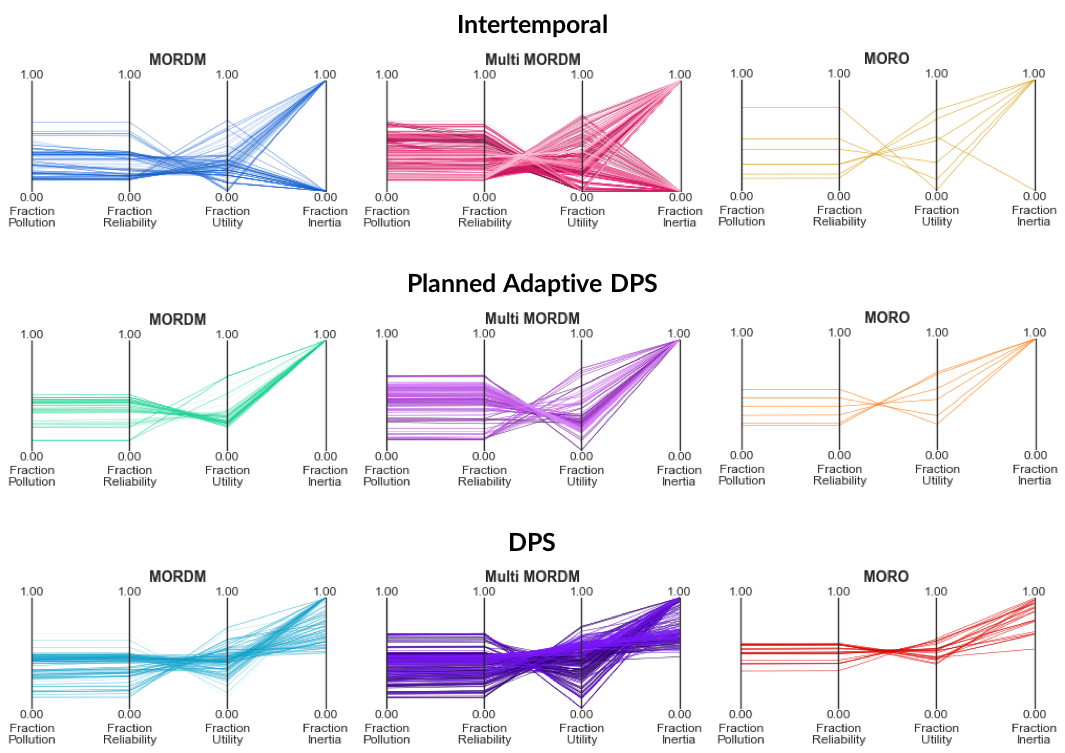
\includegraphics[width=\textwidth]{uncertainty/robust_parallel_all}
    \caption[Robustness value ranges across all pairings.]{Robustness values for policy alternatives across all model and method pairings. Robustness is determined using Starr's domain criterion \citep{Starr1963}. The desirable robustness value is at the top of each axis.}
    \label{fig:robust-parallel-all}
\end{figure}

These plots reveal that all policy alternatives for the planned adaptive DPS lake problem have high levels of inertia-based robustness. They also indicate the primary conflict between the selected outcomes of interest: there is a distinct crossing point between the reliability and utility axes for most, if not all policy alternatives across the board. This would indicate that those two outcomes of interest are generally in conflict with each other. The parallel plot can also reveal outcomes of interest that support one-another through horizontal curves that connect two axes. This is the case with the pollution and reliability outcomes of interest. Both of these trends follow the definitions of each outcome. Both the pollution and reliability metrics reflect on a desire to maintain low or manageable levels of pollution in the lake. And given that utility reflects the desire for industry and agriculture to release pollution into the lake in order to increase their profits, a conflict with the reliability and pollution metrics is expected. 

\begin{figure}[ht]
    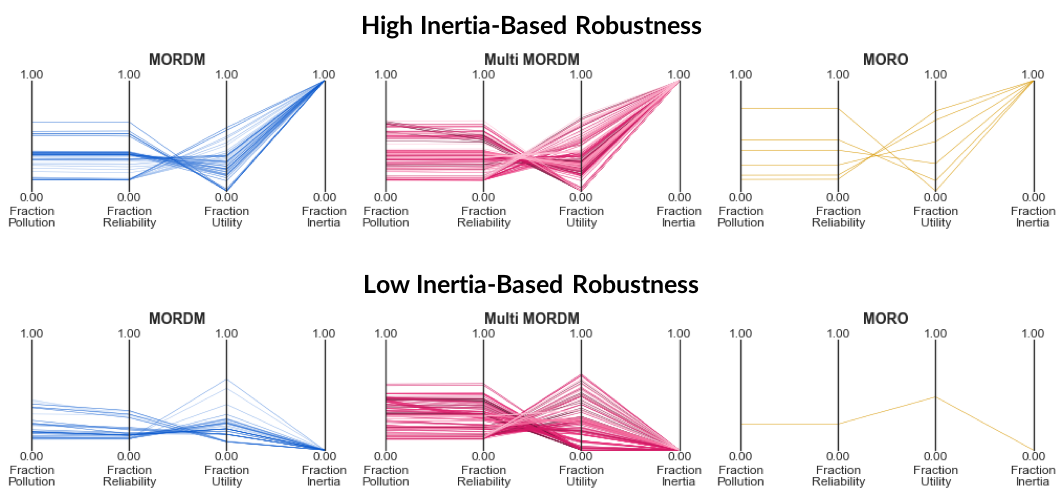
\includegraphics[width=\textwidth]{uncertainty/robust_parallel_moro_inertia}
    \caption{Robust outcome values for the intertemporal lake problem, isolating high and low inertia values.}
    \label{fig:robust-parallel-moro-inertia}
\end{figure}

Interestingly, the non-dominated policy alternatives selected for the intertemporal lake problem result in a wide range of robustness results for inertia that is not seen in the DPS and planned adaptive DPS lake models. Furthermore, the two extremes of inertia seem to be paired with utility robustness values that span the entire active value range. Separating policies that lead to high and low inertia, seen in \cref{fig:robust-parallel-moro-inertia}, does not lead to an obvious trend in robustness values that may indicate common behavior that leads to inertia that is consistently above or below the defined threshold. This type of discovery is what the next step, scenario discovery, is meant to explore and, hopefully, explain.

%TODO EEB scenario discovery on this property in an effort to determine why that happens. 

\section{Step 4: Scenario Discovery} \label{results-step4}
The final component of an RDM analysis as defined by this study is scenario discovery, which involves using PRIM to discover lingering vulnerabilities in the model after the initial search for theoretically robust alternatives. Unlike traditional RDM, which uses the information learned about lingering vulnerabilities to readjust the set of policy alternatives under consideration, these robust decision support methods must return to the model specification step to adjust decision levers or other model characteristics. Only then will the MOEA be able to determine new policy alternatives that may address the vulnerabilities identified. 

Once uncertainty analysis has been completed, the data set generated can be used for scenario discovery. Because this study uses PRIM, the first configuration step involves determining which entries in the data set are of interest. The threshold values of robustness are used here, where an entry is considered of interest if the outcome under consideration falls below its robustness threshold. The scenario discovery process will examine uncertainties in isolation, to determine what ranges of uncertainties may contribute to failure, independent of the policy in effect. Also under consideration is the potential effect of both uncertainties and lever values together, which provides an indication of a common lever and uncertainty pairing that leads to vulnerabilities in the system under consideration. Because the intertemporal variation involves so many decision levers, the policy name is used instead of the set of decision levers to simplify PRIM's search process and to provide a more straightforward way to communicate whether or not a policy impacts the system's vulnerabilities. 

The scenario discovery results for every method and lake problem pairing have indicated that there is no simple rule that explains failure in utility or inertia, given the classification settings used. Each MORDM-based study found that undesirable reliability and pollution outcomes are caused by a range of values for the pollution rate of removal, $b$. \cref{fig:mordm-PRIM} indicates the box limits and quasi-p value (in parenthesis next to the parameter name) for each application of the MORDM method that supports this conclusion. The scenario discovery results for multi-scenario MORDM based analysis and MORO based analysis reach similar conclusions, but with slight variations in the range of values for $b$ that are considered explanatory. 

\begin{figure}[ht]
    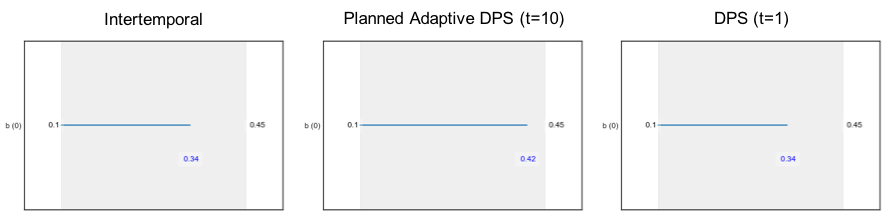
\includegraphics[width=\textwidth]{scenariodiscovery/allmordm_inspect}
    \caption[Results of PRIM Analysis]{Results of the PRIM analysis of the MORDM method applied to each variation of the lake problem. Each figure indicates the box limits when attempting to explain failures of the combined set of outcomes. Failure is indicated when an experiment does not produce an outcome of interest above the robustness threshold defined in \cref{step0-robust}.} 
    \label{fig:mordm-PRIM}
\end{figure}

This scenario discovery process can be enhanced by considering varying thresholds for each outcome of interest, to determine potential causes for different levels of failure. For example, despite not finding any explanatory behavior that caused failure in utility or inertia when classification uses the original robustness threshold, there may be ranges of uncertainties or decision levers that explain failure when robustness does not meet a lower standard (i.e. there are fewer failures to meet the desired utility or inertia setting). By selecting a smaller group of experiments that are of interest, PRIM may prove more effective, as it has been known to struggle with larger sets of experiments that are of interest \citep{Kwakkel2017}. 
\newcounter{comparison} \setcounter{comparison}{1}

\chapter{Comparison of Results}\label{chapter-comparison}

\begin{abstract}
     This chapter will analyze and compare the results of each method and model variation pairing, according to the comparison metrics established in \cref{dev-comparisons}. In the same way that \cref{dev-comparisons} separated metrics into three main categories, the comparisons will also be discussed in three primary sections. The first, \cref{results-compare-complexity}, will discuss the two identified comparison methods that involve the setup needs for each method. Next, \cref{results-compare-communication} will cover the metrics related to method communication. Finally, the results themselves will be compared in \cref{results-compare-results}. 
\end{abstract}

\newpage

\section{Setup Complexity}\label{results-compare-complexity}
    \subsection{Comparison \thecomparison : Complexity of problem setup}\stepcounter{comparison}
    Based on the definition of this metric in \cref{dev-comparisons}, problem setup involves two components: setup requirements that are identified by method structure and setup requirements specific to the tooling used to perform an analysis. Because the three methods considered in this study are all based on an RDM structure, the requirements for model specification are the same. Each follows the XLRM structure that supports a series of uncertainties and levers connected through relationships to the identified outcomes of interest. Therefore, there is no significant difference in terms of method-required problem setup. 
    
    The second element of problem setup relates to the requirements of any software packages that are used to execute analysis. For example, a tool like OpenMORDM provides a well-structured implementation of the MORDM method, which can also support multi-scenario MORDM, but is not able to support the functionality required for MORO \citep{Hadka2015}. Given that multi-objective robust optimization has not yet been presented as a formal RDM-based method in literature until now, there is no well-structured package similar to OpenMORDM for MORO. 
    
    This study makes use of the Exploratory Modelling and Analysis (EMA) Workbench for all three methods, which provides a highly customization interface with which to implement the steps required for all methods \citep{Kwakkel2017}. This package is not as precisely structured as OpenMORDM, which provides for a higher level of customization and flexibility, but correspondingly requires more work to establish the required configuration. Because this package is able to support all three methods considered in this study, model configuration is similar. The differences lie in the lake problem variations themselves. The EMA Workbench provides native support for several model implementations, including Vensim, NetLogo, and Python, which is the implementation used in this study. The Python implementations require uncertainties and decision levers to be specified as individual parameters of the method function. This process can get unwieldy given a large number of uncertainties and levers, as in the case of the intertemporal lake problem, but is quite straightforward. 
    
    \begin{comparisonbox}{Summary: Complexity of Problem Setup}
        The fact that the methods considered all have a foundation in robust decision making, and that the same software package can be used for each method, means that there is no significant differences in the complexity of problem setup. 
    \end{comparisonbox}

    \subsection{Comparison \thecomparison : Complexity of method setup}\stepcounter{comparison}
    The complexity of method setup refers primarily to the effort involved in steps 2-4 of the RDM process. Because steps 3 and 4 are common to all three methods, setup for these will not be compared here. The difference in each method lies in the policy alternative determination, or search phase, and specifically in two elements of the search phase that make each method unique. 
    
    The first is the manner in which data is gathered to compare potential policy alternatives, which will be referred to as the reference scenario or scenarios. With respect to MORDM, this is quite straightforward: a single predefined reference scenario is used, called the base reference scenario. The work required to setup alternative comparison is also quite straightforward in MORO, where a constant and small ensemble of uncertainty vectors is used throughout the entire search. This only requires a sampling across the uncertainty space that is already defined in model specification. As described in \cref{dev-step2}, Latin Hypercube Sampling was used to build this small ensemble, which is a well-established sampling technique built into EMA Workbench. By leveraging built in sampling functionality, the effort required to set up the alternative comparison component of the search remains quite small for MORO. 
    
    Reference scenario configuration is more complex in multi-scenario MORDM, as this method involves the specification of multiple scenarios that are independently used to locate potentially robust policy alternatives. As discussed in \cref{step2-scenarios}, there are many possible ways to select scenarios. If the analyst decides to use a random set of scenarios selected from a large ensemble of uncertainty settings, or if those scenarios are determined exclusively through decision maker input, the reference scenario selection process does not significantly add to the complexity of setup for multi-scenario MORDM. 
    
    This study uses a significantly more time intensive method of selection that requires the completion of an MORDM analysis before selecting reference scenarios. In the initial MORDM run, scenario discovery is used to determine the boundaries of vulnerability that remain in that discovered set of policy alternatives. Once those boundaries are determined, that information is used to select a set of maximally diverse alternatives from within those boundaries. This involves first building a larger ensemble of uncertainty vectors and selecting those vectors that fall within the vulnerable range. Then, an exhaustive search is used from within the identified group to determine which set of uncertainty vectors are maximally diverse. As this is an exhaustive search, each possible combination of policies must be examined. This process can get extremely computationally expensive very quickly, as indicated by \cref{fig:trend-policycombinations}. As the size of the set of uncertainty vectors with which to select a set of reference scenarios from increases, the number of combinations of maximally diverse policy alternatives grows exponentially. This computational cost has a significant impact on the cost and complexity of the search phase in multi-scenario MORDM. 
    
    \begin{figure}[ht]
        \centering
        \captionsetup{width=0.5\textwidth}
        
        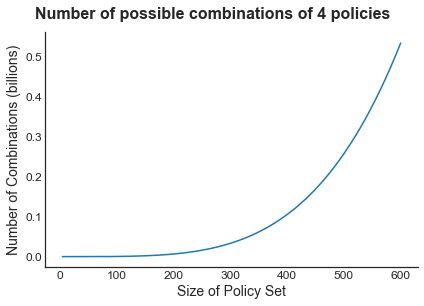
\includegraphics[width=0.5\textwidth]{compare/trend_combinations}
        \caption[Trend in computational cost when selecting maximally diverse policies]{The number of possible combinations of 4 policies given a set of available policies. This demonstrates the rapid increase of combinations and therefore of computational cost when determining maximally diverse scenarios.}
        \label{fig:trend-policycombinations}
    \end{figure}

    The second configuration element of the search phase is the manner in which policies are compared. Both MORDM and multi-scenario MORDM use the same outcome definitions as in the model specification phase, requiring no additional configuration work. MORO requires a custom comparison definition, which depends on the robustness method used. If it involves a comparison to another specific scenario (worst or best case performance, for example), then that worst or best case scenario must be found before the search can begin. If the robustness metric instead looks at performance below a threshold, as in the case of this study, then the comparison definition involves defining how to compare each outcome to the relevant threshold in order to begin the search. 
    
    \begin{comparisonbox}{Summary: Complexity of Method Setup}
        The elements of setup complexity are summarized in \cref{table:setupcomplexity}. This table provides a quick view of the differences in the two interesting elements of configuration for the search phase. The value in parentheses indicates the effort required for this study, specifically. So, for this study, multi-scenario MORDM involves the most complexity with respect to method setup. 
    \end{comparisonbox}
    
    \begin{table}[ht]
        \centering
        \captionsetup{width=0.70\textwidth}
        \caption[Setup Complexity of Methods]{Complexity of configuration in the policy alternative determination phase. Effort provides a qualitative idea of the amount of work required to configure the search, given an already specified model. }
        \label{table:setupcomplexity}
        
        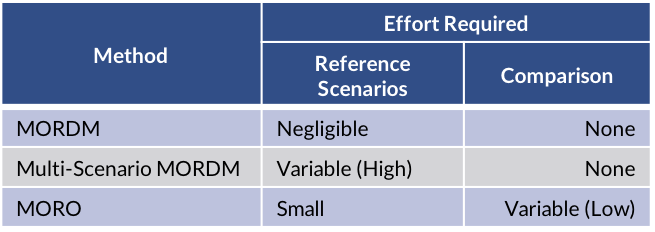
\includegraphics[width=0.7\textwidth]{compare/complexity_table}
    \end{table}
        
\section{Communication}\label{results-compare-communication}
    \subsection{Comparison \thecomparison : Results communication} \stepcounter{comparison}
    As described in \cref{dev-comparisons}, results communication refers to the way in which each method communicates results during execution. In the case of this study, each method considered is following the same RDM-based structure. Correspondingly, results communication is common across each of the methods. For review, the communication of each step is described here. The first step, model specification, involves setup for the following three RDM phases, and so does not involve communication of any results. The end of step 2, policy alternative determination, involves the reporting of the complete set of potentially robust policy alternatives that will be used in the remaining two steps. At this point in the analysis, therefore, analysts and decision makers will know the set of alternatives that has been identified. In the remaining two steps of the analysis, more information about the policy alternatives, including the assessed robustness of each alternative when considering a wide array of potential future states of the world in step 3 and remaining vulnerabilities that the alternatives still have in step 4. 
    
    \begin{comparisonbox}{Summary: Results Communication}
        Results communication is common across all three methods. Policy alternatives are reported in step 2 of each method, the robustness of each alternative is revealed in step 3, and potential vulnerabilities are communicated at the conclusion of step 4, scenario discovery.
    \end{comparisonbox}
    
    \subsection{Comparison \thecomparison : Robustness communication} \stepcounter{comparison}
    Each method, based on the RDM structure, is able to use the same robustness metric to determine policy robustness in the uncertainty analysis stage, so there is no method-specific difference in robustness communication. As this is then dependent on the robustness metric selected, it is not applicable to this study, which is focusing on the impact of selection of a robust decision support method on the analysis process. 
    
    \begin{comparisonbox}{Summary: Robustness Communication}
        The robustness metric used is common across all three methods, and therefore there is no difference in robustness communication for this study. 
    \end{comparisonbox}

    \subsection{Comparison \thecomparison : Ease of results updating if model specification changes} \stepcounter{comparison}
    The impact of a change in model specification will be explored for steps 2-3 of each robust decision support method. Fundamentally, a change in model specification will impact all methods in a similar way, due to the fact that they each follow the same basic RDM structure. The decision about how much of the process should be repeated relates more to decision maker goals, as described below. 
    
    \textbf{Step 2: Policy Alternative Determination}: For every method, a change in method specification will require a complete restart of the search process in the policy alternative determination phase, especially if the analyst or decision makers think that the change will have a significant impact on the resulting set of non-dominated policy alternatives. 
    
    \textbf{Step 3: Uncertainty Analysis}: If decision makers are primarily interested in how these changes will affect the robustness of an existing set of non-dominated policy sets, a specification change need only lead to a new ensemble of uncertainty settings with which to test the efficacy of each policy alternative. Again, this is common to all methods that are being studied here.
    
    \textbf{Step 4: Scenario Discovery}: A change in model specification does not directly result in an alteration to the scenario discovery process. It is impacted through changes to the previous two steps of analysis and must be reran to determine the impact of specification changes on any previously identified vulnerable regions.
    
    \begin{comparisonbox}{Summary: Ease of results updating if model specification changes}
         The impact of a change in the model specification affects all three methods under consideration in the same way. Updates may be required in steps 2 or 3 depending on they type of change and decision maker goals.
    \end{comparisonbox}
    
    \subsection{Comparison \thecomparison : Ease of results updating if robustness metric changes} \stepcounter{comparison}
    The impact of a change in the robustness metric will be explored for steps 2-3 of each robust decision support method. Fundamentally, a change in robustness metric most affects the uncertainty analysis step. However, because MORO directly incorporates robustness into the policy analysis determination process, a change in robustness metric may also force a re-run of that step as well. 
    
    \textbf{Step 2: Policy Alternative Determination}: A change in robustness metric will have no impact on this step for MORDM. Because the MORO method incorporates robustness into the search process, if the change relates to the definition of robustness used to sort policy alternatives, a change in robustness metric demands that the search process be repeated. 
    
    It is also possible that a change in robustness metric will impact multi-scenario MORDM. Because such a change may affect what is identified as a vulnerable region in the scenario discovery process of an MORDM analysis, the range with which to select a set of reference scenarios from may change for the multi-scenario MORDM analysis. Such a change would require a complete restart of the search process for each newly identified reference scenario.
        
    \textbf{Step 3: Uncertainty Analysis}: For all methods, a change in the robustness metric will not force a repeat of the computational exploration phase of uncertainty analysis, which simply builds a large data set that indicates the performance of each policy alternative over a wide range of potential states of the world. A change in the robustness metric would require recalculation of the robustness of each policy at this stage for each decision support method. 
    
    \textbf{Step 4: Scenario Discovery}: This step will be directly affected by a change in robustness metric if that change results in a different definition of which policy and uncertainty sets lead to "interesting" outcome values. For example, in the case of a domain criterion metric, a change in threshold value may affect how "interesting" data points are identified. For the most part, though, scenario discovery will be repeated based on changes in the search phase or uncertainty analysis. 

    \begin{comparisonbox}{Summary: Ease of results updating if robustness metric changes}
        As the robustness metric is common for all three methods, a change in robustness metric requires the recalculation of the robustness of each policy alternative in Step 2: Uncertainty Analysis for all. Furthermore, because MORO uses robustness to compare policy alternatives in the search phase, a change in the definition of robustness there will require a total restart of the search phase. 
    \end{comparisonbox}

\section{Results}\label{results-compare-results}
    \subsection{Comparison \thecomparison : Computational cost} \stepcounter{comparison}
    The comparison of computational cost will primarily consider the number of model executions required to complete the policy alternative determination step of each method. Also discussed is the computational cost of uncertainty analysis, which revolves around the number of model evaluations required to build the complete data set of experiments (where an experiment is the sets of uncertainty and lever values, and associated outcomes of interest). 
    
    \begin{table}[t!]
    \captionsetup{width=\textwidth}
    \caption[Computational cost for all pairings]{Computational cost determined for each model variation and method pairing. Total computational cost, calculated as number of model function executions, can be found in the last rows.}
        
    \begin{subtable}{\textwidth}
        \centering
        \captionsetup{width=\textwidth}
        \caption{Step 2: Policy Alternative Determination}
        \label{table:computationalcost}
        
        \rowcolors{2}{odd-row-blue}{even-row-blue}
        \setlength\arrayrulewidth{1pt}\arrayrulecolor{white}
        \begin{tabularx}{\textwidth}{l|l|R|R|R}
            \hline
            \rowcolor{tudelft-dark-blue!80}
            \multicolumn{2}{l|}{\color{white} \textbf{}} 
            & \multicolumn{1}{c|}{\color{white} \textbf{MORDM}} 
            & \multicolumn{1}{c|}{\color{white} \textbf{\begin{tabular}[c]{@{}c@{}}Multi-\\ Scenario \\ MORDM\end{tabular}}}
            & \multicolumn{1}{c}{\color{white} \textbf{MORO}} \\ \hline
            
            \cellcolor{even-row-blue}   & Intertemporal    & 500,000   & 500,000  &  300,000    \\ \cline{2-5} 
            \cellcolor{even-row-blue}   & \cellcolor{odd-row-blue}Planned Adaptive &
            \cellcolor{odd-row-blue}100,000   & \cellcolor{odd-row-blue}100,000  & \cellcolor{odd-row-blue}100,000     \\ \cline{2-5} 
            \multirow{-3}{*}{\cellcolor{even-row-blue}\begin{tabular}[c]{@{}l@{}}Number of \\ Function \\ Executions (NFE)\end{tabular}} & DPS             & 100,000   & 100,000  & 100,000      \\ \hline
            
            \multicolumn{2}{l|}{\cellcolor{odd-row-blue}Per Policy Executions} & 1 & 1 & 50 \\ \hline
            \multicolumn{2}{l|}{\cellcolor{even-row-blue}Search Repetitions} & 1 & 5 & 1 \\
            
            \noalign{\global\arrayrulewidth=4pt} \arrayrulecolor{tudelft-dark-blue!80}
            \hline
            \noalign{\global\arrayrulewidth=1pt} \arrayrulecolor{white}
            
            \cellcolor{odd-row-blue}    
            & \textbf{Intertemporal}    & 500,000  & 2,500,000 & 15,000,000  \\ \cline{2-5} 
            \cellcolor{odd-row-blue} 
            & \cellcolor{even-row-blue}\textbf{Planned Adaptive} & \cellcolor{even-row-blue}100,000  & \cellcolor{even-row-blue}500,000   & \cellcolor{even-row-blue}5,000,000    \\ \cline{2-5} 
            \multirow{-3}{*}{\cellcolor{odd-row-blue}\textbf{\begin{tabular}[c]{@{}l@{}}Computational \\ Cost (NFE)\end{tabular}}}
            & \textbf{DPS}              & 100,000  & 500,000   & 5,000,000           \\ \hline
        \end{tabularx}
    \end{subtable}
    \newline
    \vspace*{0.3 cm}
    \newline
    \begin{subtable}{\textwidth}
        \centering
        \captionsetup{width=\textwidth}
        \caption{Step 3: Uncertainty Analysis}
        \label{table:cost-uncertainty}
        
        \rowcolors{2}{odd-row-blue}{even-row-blue}
        \setlength\arrayrulewidth{1pt}\arrayrulecolor{white}
        \begin{tabularx}{\textwidth}{l|l|R|R|R}
            \rowcolor{tudelft-dark-blue!80}
            \multicolumn{2}{l|}{\color{white} \textbf{}} 
            & \multicolumn{1}{c|}{\color{white} \textbf{MORDM}} 
            & \multicolumn{1}{c|}{\color{white} \textbf{\begin{tabular}[c]{@{}c@{}}Multi-\\ Scenario \\ MORDM\end{tabular}}}
            & \multicolumn{1}{c}{\color{white} \textbf{MORO}} \\ \hline
            
            \cellcolor{even-row-blue}   & Intertemporal  & 90 & 291 & 7 \\ \cline{2-5} 
            \cellcolor{even-row-blue}   & \cellcolor{odd-row-blue}Planned Adaptive &
            \cellcolor{odd-row-blue}48   & \cellcolor{odd-row-blue}113  & \cellcolor{odd-row-blue}6     \\ \cline{2-5} 
            \multirow{-3}{*}{\cellcolor{even-row-blue}\begin{tabular}[c]{@{}l@{}}Number of \\ Nondomianted \\ Alternatives\end{tabular}} & DPS             & 110 & 209 & 22 \\ \hline
            
            \multicolumn{2}{l|}{\cellcolor{odd-row-blue}Uncertainty Ensemble Size} & 10,000 & 10,000 & 10,000 \\
            
            \noalign{\global\arrayrulewidth=4pt} \arrayrulecolor{tudelft-dark-blue!80}
            \hline
            \noalign{\global\arrayrulewidth=1pt} \arrayrulecolor{white}
            
            \cellcolor{even-row-blue}   & Intertemporal  & 900,000 & 2,910,000 & 70,000 \\ \cline{2-5} 
            \cellcolor{even-row-blue}   & \cellcolor{odd-row-blue}Planned Adaptive &
            \cellcolor{odd-row-blue}480,000   & \cellcolor{odd-row-blue}1,130,000  & \cellcolor{odd-row-blue}60,000     \\ \cline{2-5} 
            \multirow{-3}{*}{\cellcolor{even-row-blue}\textbf{\begin{tabular}[c]{@{}l@{}}Computational \\ Cost (NFE)\end{tabular}}} & DPS             & 1,100,000 & 2,090,000 & 220,000 \\ \hline
        \end{tabularx}
    \end{subtable}
    \end{table}
    
    A catalog of the computational cost for the search phase can be found in \cref{table:computationalcost}. The results indicate that methods that more directly include robustness considerations incurr a larger computational cost in the search phase of analysis. Given the configuration details used, multi-scenario MORDM is 5 times more expensive than MORDM (because 5 scenarios are considered here), and MORO is 50 times more expensive, based on the use of an ensemble of 50 uncertainty settings in the search process. Therefore, computational cost in this step seems to incorporate a trade-off between efficiency and robustness. 
    
    There is also a variation in computational cost in step 3, based on the size of each set of non-dominated policy alternatives. As \cref{table:cost-uncertainty} indicates, multi-scenario MORDM appears to have the largest computational cost in uncertainty analysis due to the larger number of non-dominated alternatives identified through 5 separate reference scenarios.
    
    The translation of computational cost to physical processing time is not consistent for both steps. There is additional work outside of model execution in the search phase that also contribute to processing time. The MOEA used in this study involves a non-dominated epsilon sort after every generation. This sorting stage takes more time with larger sets of non-dominated alternatives, due to the need for more comparisons each time. It does still contribute a smaller fraction to the total processing time than model execution, so despite sorting taking longer for MORDM due to the larger sets of non-dominated solutions, the overall search process for MORO still takes much longer in total. The uncertainty analysis does not have the same addition of processing time, so physical processing time will be less per model execution
    
    \begin{comparisonbox}{Summary: Computational cost}
        Analysis using MORO has a significantly higher computational cost when compared to the other two methods. Because multi-scenario MORDM involves repeating an MORDM analysis the number of times equal to the number of reference scenarios used (in this case 5), multi-scenario MORDM is also more computational expensive than MORDM. 
    \end{comparisonbox}

    \subsection{Comparison \thecomparison : Convergence of search} \stepcounter{comparison}
    Convergence of an MOEA-based search, as discussed in \cref{results-convergence}, tracks the stabilization of the search for policy alternatives. \cref{fig:compare-convergence} directly compares the epsilon progress and hypervolume convergence trends of each method for a specific model variation. In these plots, a single line represents the mean across all repetitions of the search for each method. In the case of multi-scenario MORDM, each line of the color shown in the legend represents the search for one of the reference scenarios used. For clarity, the multi-scenario MORDM search involving the base reference scenario is left out, as its convergence matches convergence of the MORDM-based search.
    
    There is a difference in mean hypervolume convergence for the intertemporal + MORO pairing as compared to the other two methods. Both epsilon progress and hypervolume stabilize more slowly. This indicates that the minimum number of function executions to ensure stability is higher when using the MORO method for the intertemporal lake problem. It is possible that difference is due to the small size of the set of non-dominated alternatives (6) as compared to the number of decision levers involved (100). The hypervolume of such a small set of alternatives with so many levers can be more significantly impacted by additions or alterations to the set. Furthermore, as changes hypervolume indicate that new policies are being added to the set of non-dominated alternatives, it follows that epsilon progress will have a similarly slower time to convergence. 
    
    The other data point of interest is the epsilon progress of the MORDM-based search with respect to the DPS lake problem variation. Though the epsilon progress here seems to stabilize much more slowly, because the hypervolume convergence is not significantly different, the search process does not seem to be adding policy alternatives that increase the diversity of the non-dominated policy set. When a newly found alternative does not increase diversity of the non-dominated set, no significantly different alternative courses of action are being added to consideration. Therefore, the difference in epsilon progress can be discounted and the stabilization of hypervolume convergence with respect to the DPS + MORDM pairing would seem to have a similar rate of stabilization to the other two pairings involving the DPS model variation. 
    
    There is no significant difference in the convergence of an MOEA-based search when considering the planned adaptive DPS model variation. Each of the methods stabilize at a similar point in the search process in this case. This indicates that no method considered in this study is able to analyze the planned adaptive DPS model with more efficiency than the others. 
    
    \begin{figure}[t!]
        \centering
        \captionsetup{width=\textwidth}
        
        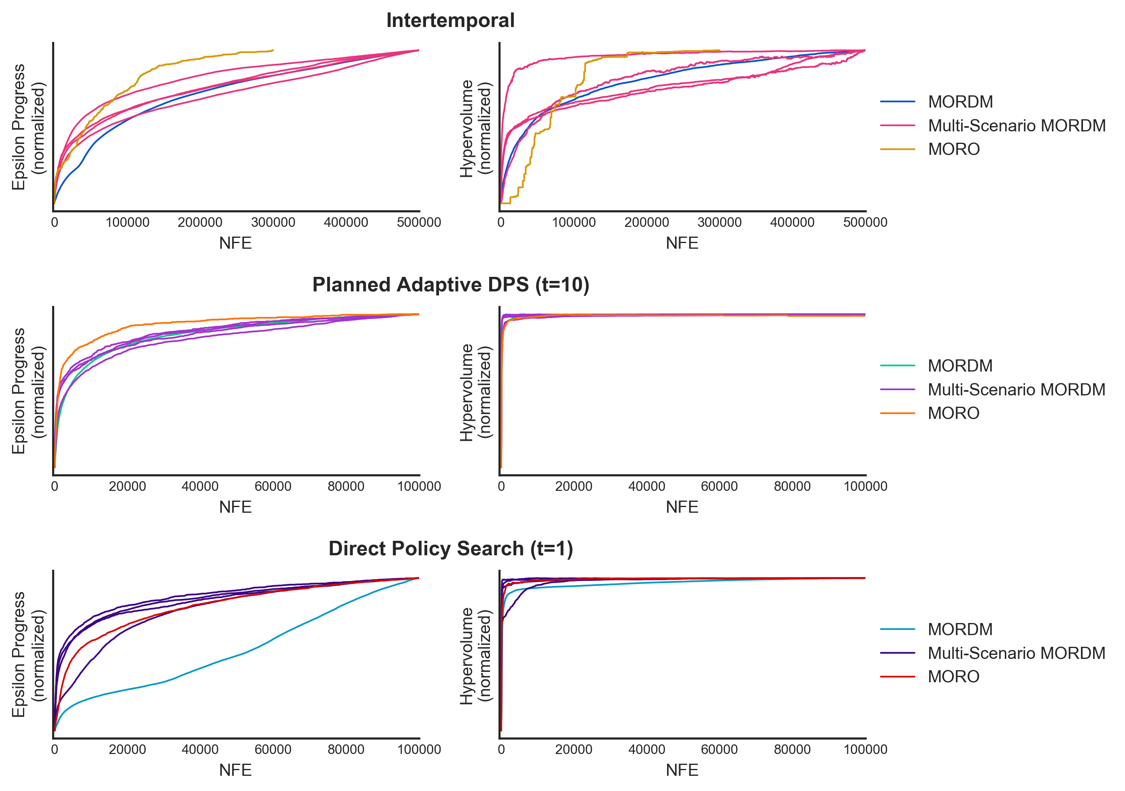
\includegraphics[width=\textwidth]{compare/convergence_normalized}
        \caption[Mean epsilon progress across all pairings and search repetitions]{Mean epsilon progress and hypervolume convergence per model variation and method pairing. Normalized with respect to the maximum value within an individual search process.}
        \label{fig:compare-convergence}
    \end{figure}
    
    \begin{comparisonbox}{Summary: Convergence of search}
        In the case of the planned adaptive DPS model variation, search convergence is very similar across all three methods. The same can be said for the DPS variation, given that the epsilon progress differences for the MORDM method appear to not lead to an increased diversity of the non-dominated set of alternatives, and therefore do not uncover previously unknown combinations of potentially robust decision lever settings. Finally, MORO seems to stabilize more slowly for the intertemporal variation, possibly due to the combination of a large number of decision levers and small size of set of the non-dominated policy alternatives. 
    \end{comparisonbox}
    
    \subsection{Comparison \thecomparison : Robustness of recommended policy set} \stepcounter{comparison}
    As a reminder, this comparison involves examining the overall robustness values for each model variation and method pairing. \cref{fig:robust-heatmap-mean} shows an overall picture of the mean robustness values for each outcome of interest across pairings.
    
    \begin{figure}[ht]
        \centering
        \captionsetup{width=0.8\textwidth}
        
        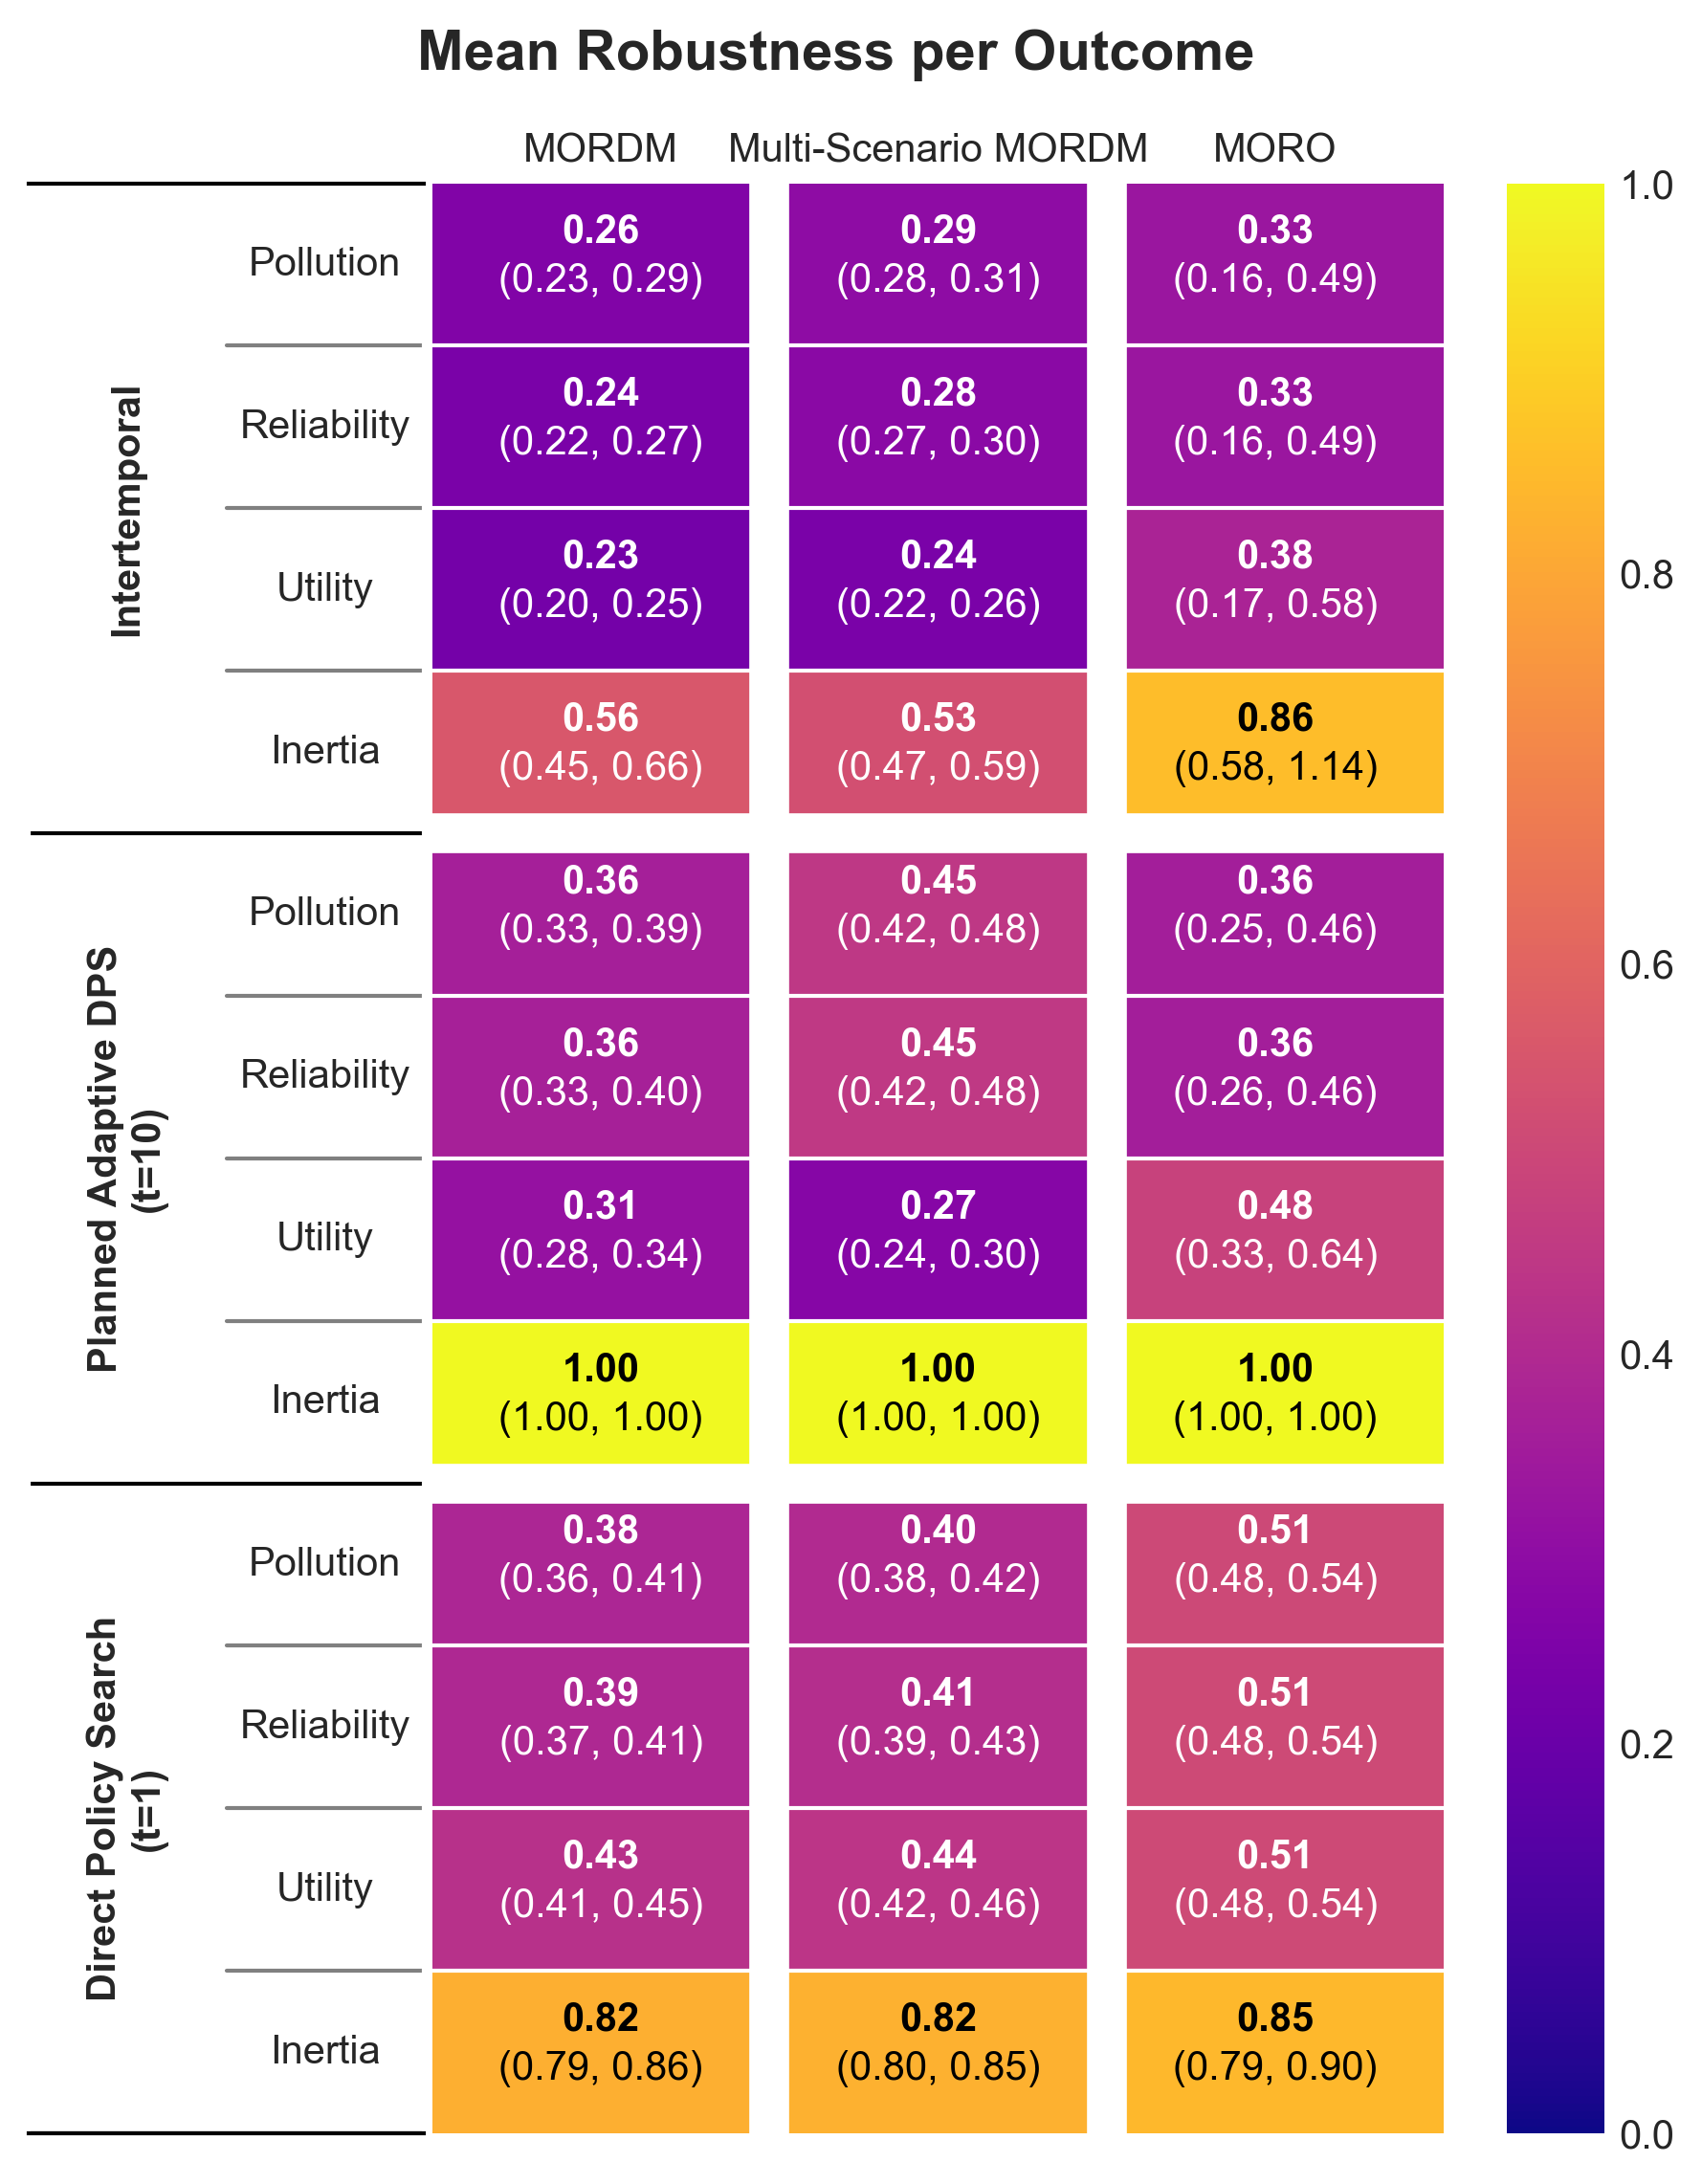
\includegraphics[width=0.8\textwidth]{compare/robust_heatmap_mean}
        \caption[Heatmap of mean robustness across all pairings.]{Mean robustness per model variation and method pairing. This heat map is annotated to include the bounds of the 95 percent confidence interval surrounding the mean.}
        \label{fig:robust-heatmap-mean}
    \end{figure}
    
    The intertemporal and DPS model variations show a general trend of increasing mean robustness from MORDM to MORO, which confirms that the more robustness is incorporated into the search process, the more robust the resulting policy alternatives will be. 
    
    Unlike the intertemporal and DPS model variations, however, the planned adaptive DPS variation shows a sharp increase in robustness of pollution level and reliability, along with a drop in utility from MORDM to multi-scenario MORDM. No increase in robustness of pollution and reliability is seen with respect to the MORDM and MORO methods, also unlike the results seen with the other two variations. Inertia remains constant in this case, with perfect robustness. This result is expected because inertia relates to the consistency of the release decision, and as the release decision changes only every 10 time steps in the planned adaptive DPS variation, inertia of those policies will be high. 
    
    Given that there seems to be an inverse relationship between the pollution or reliability outcomes and utility, it is expected that an increase in the robustness of the first two is associated with a decrease in robustness of the last (\cref{results-step3}). The question then becomes a matter of what caused the change in behavior of robustness in the case of the planned adaptive DPS model variation. 
    
    Examining the release rules that are configured using decision lever values sheds some light onto the potential reason for the different robustness behavior in the case of the planned adaptive DPS model. \cref{fig:release-rules} plots the release rules of the non-dominated policy alternatives for both the DPS and planned adaptive DPS variations and for all three robust decision support methods. These rules show the amount of pollution that would be released for a variety of existing pollution concentrations, as defined by \cref{eq:release-rules} \citep{Quinn2017}. 
    
    \begin{equation}\label{eq:release-rules}
        \alpha_{t} = \frac{X_{t-1}^{q}}{(1+X_{t-1}^{q})} - b*X_{t}
    \end{equation}
    
    \begin{figure}[ht]
        \centering
        \captionsetup{width=\textwidth}
        
        \begin{subfigure}[b]{\textwidth}
            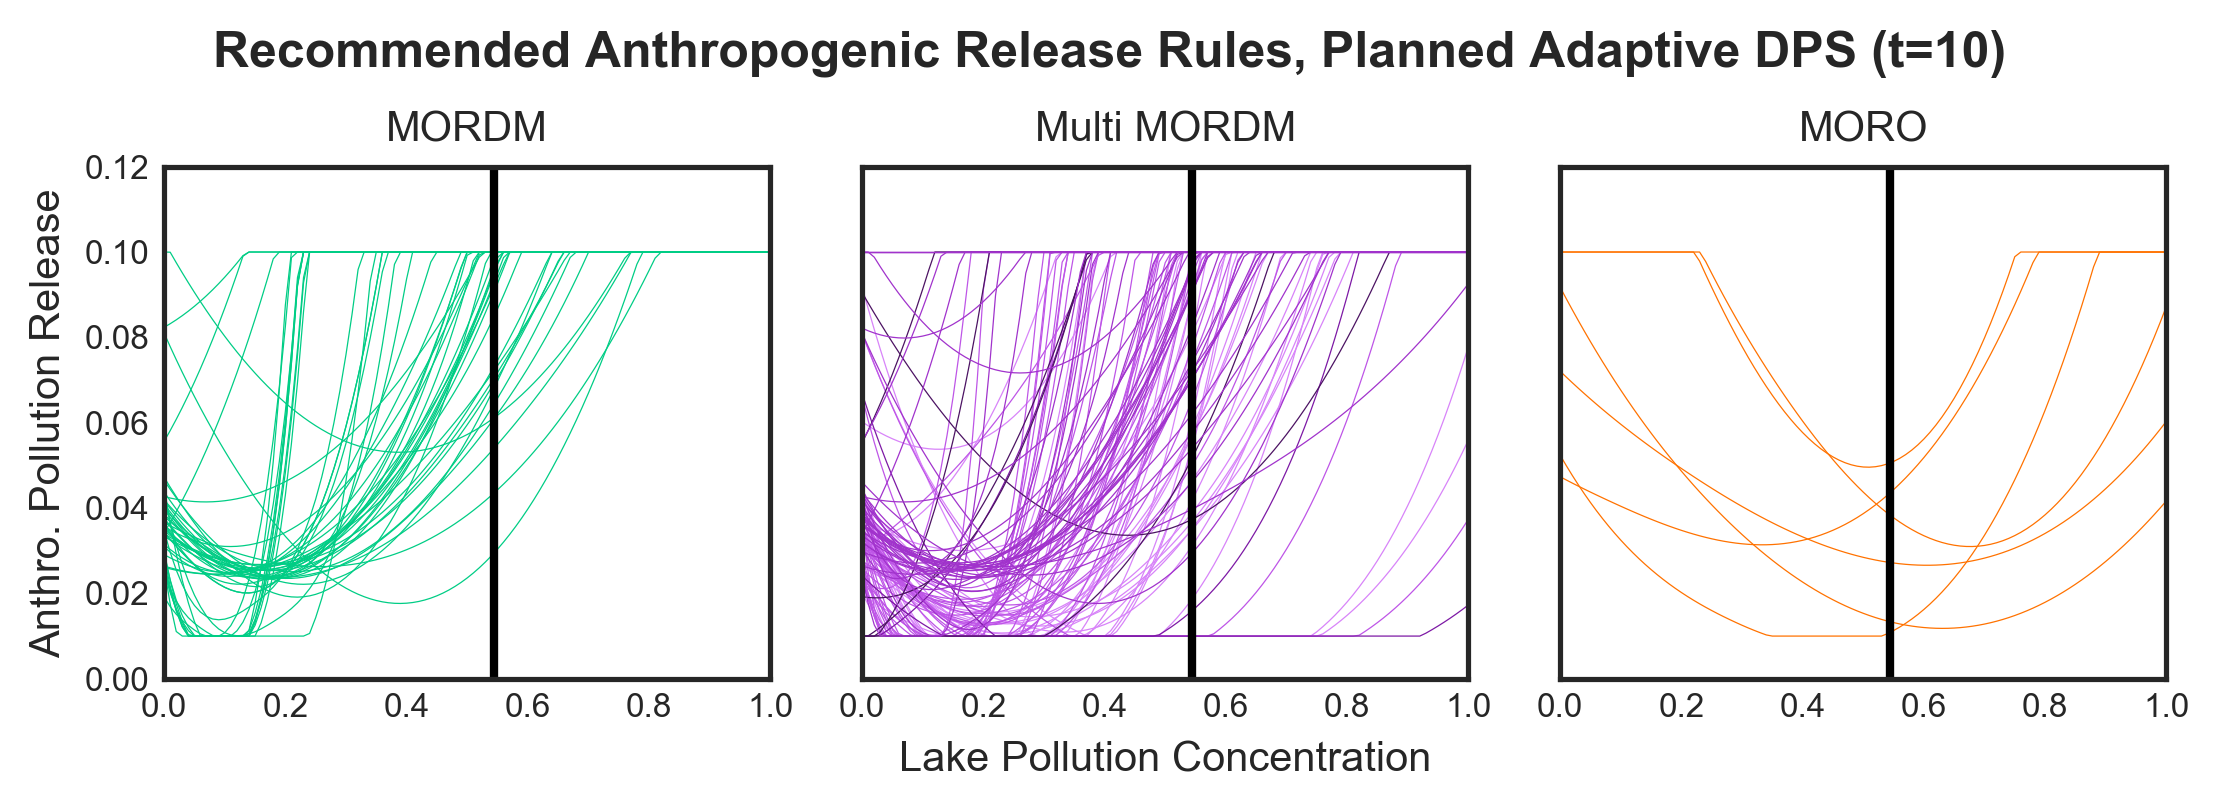
\includegraphics[width=\textwidth]{compare/rules_plannedadaptive_highres}
            \label{fig:planned-releaserules}
        \end{subfigure}
    
        \begin{subfigure}[b]{\textwidth}
            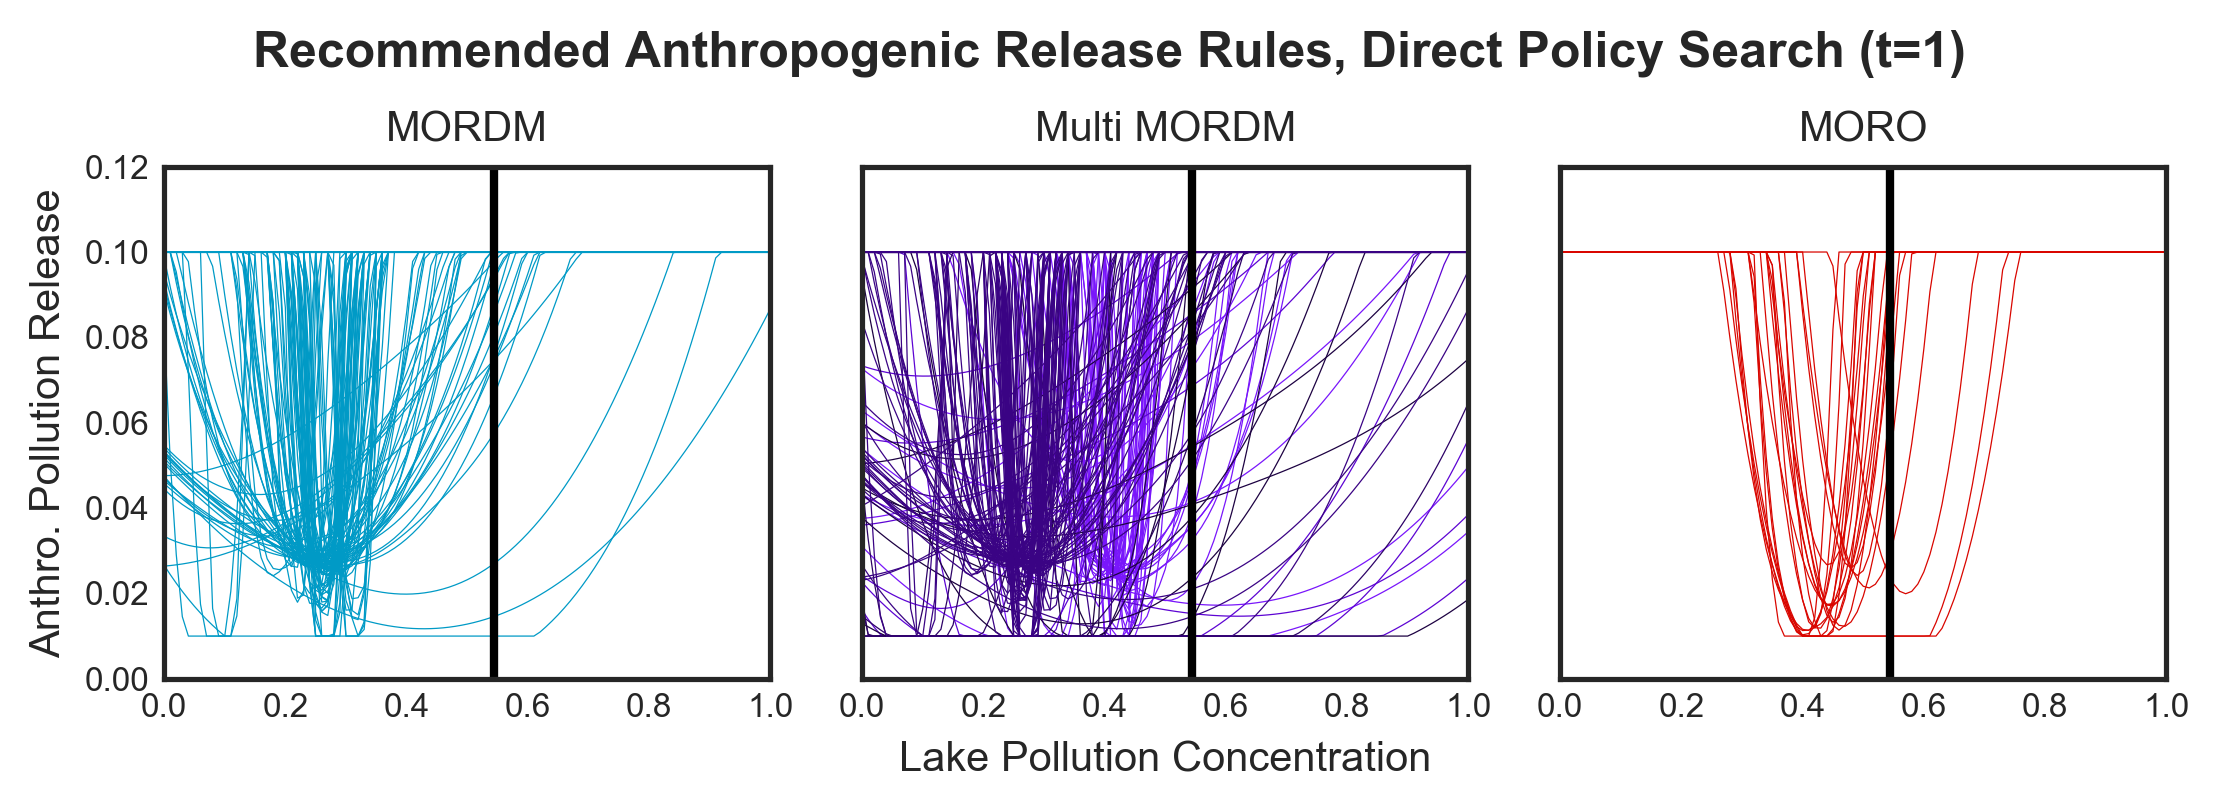
\includegraphics[width=\textwidth]{compare/rules_dps_highres}
            \label{fig:dps-releaserules}
        \end{subfigure}
        
        \caption[Release rules for DPS and planned adaptive DPS variatons]{Release rules for the DPS and Planned Adaptive DPS model variations. The vertical black line indicates the critical pollution level for the reference uncertainty settings (b=0.42, q=2.0).}
        \label{fig:release-rules}
    \end{figure}

    This information indicates that the policy alternatives found through a Multi-MORDM search, especially, produce much more conservative pollution release decisions when compared to the DPS variation, indicated by the pollution concentration which triggers the minimum pollution release amount (which is lower in the planned adaptive DPS variation). The more conservative policy selection would contribute to higher robustness in pollution level and reliability, as well as lower utility robustness, which is what is seen in \cref{fig:robust-heatmap-mean}. 
    
    \begin{figure}[H]
        \begin{subfigure}[b]{\textwidth}
            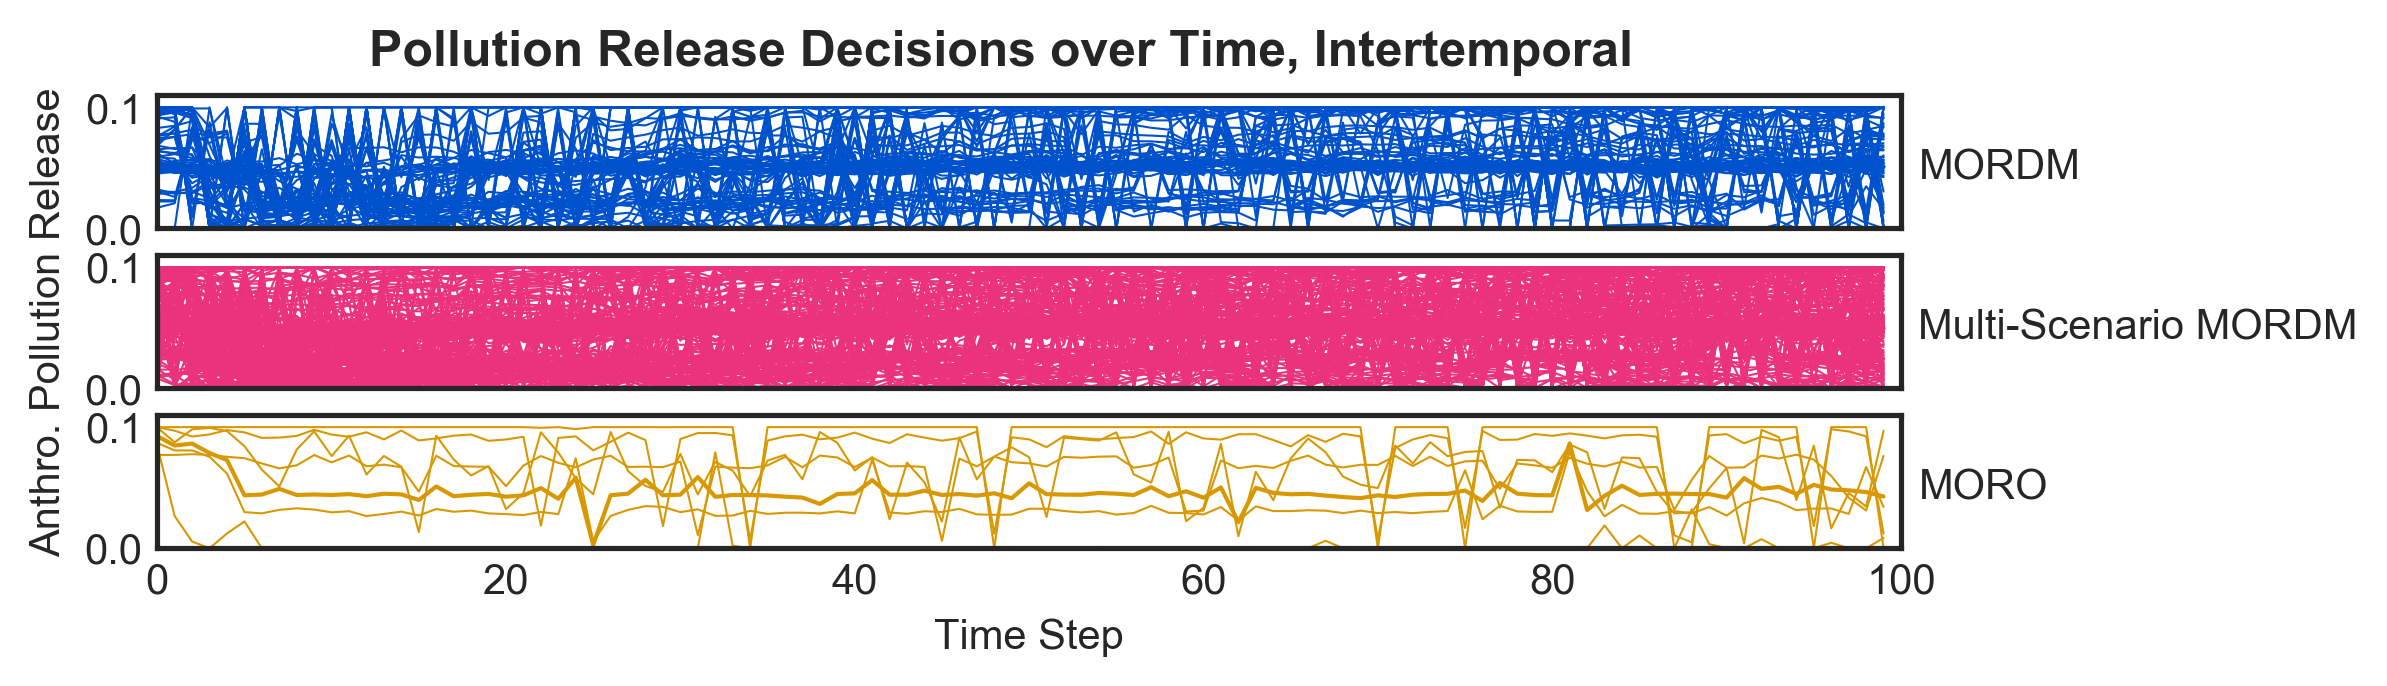
\includegraphics[width=\textwidth]{compare/overtime_intertemporal_highres}
            \label{fig:intertemporal-overtime}
        \end{subfigure}
        \begin{subfigure}[b]{\textwidth}
            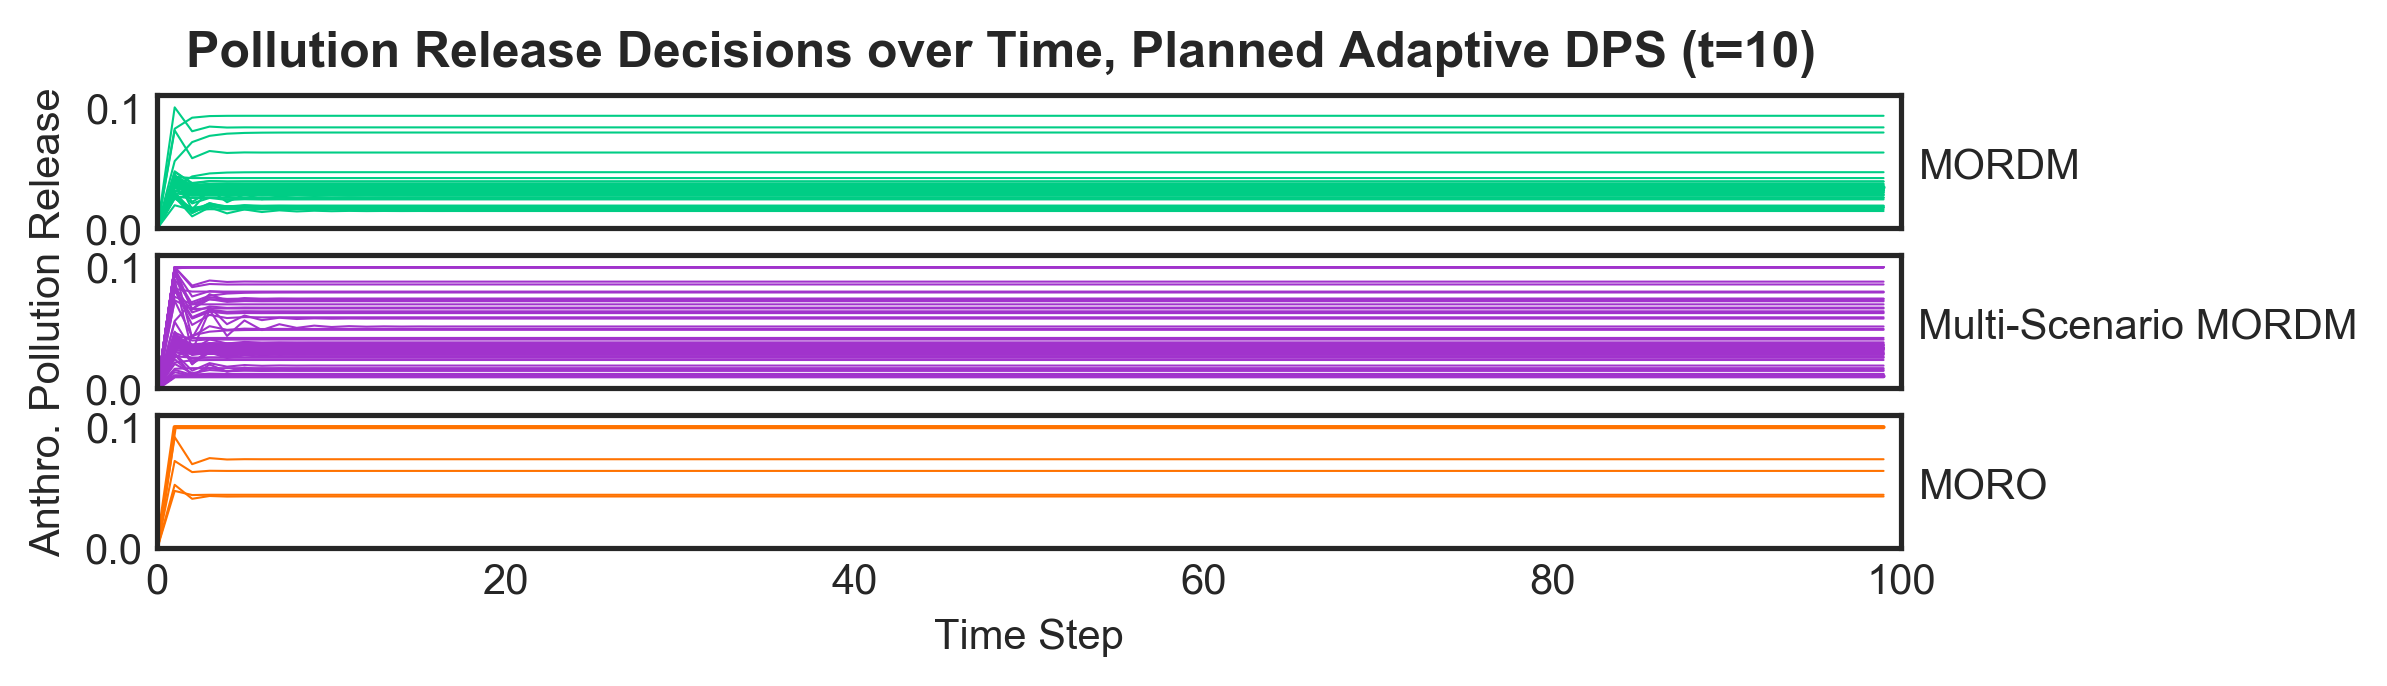
\includegraphics[width=\textwidth]{compare/overtime_plannedadaptive_highres}
            \label{fig:planned-overtime}
        \end{subfigure}
        \begin{subfigure}[b]{\textwidth}
            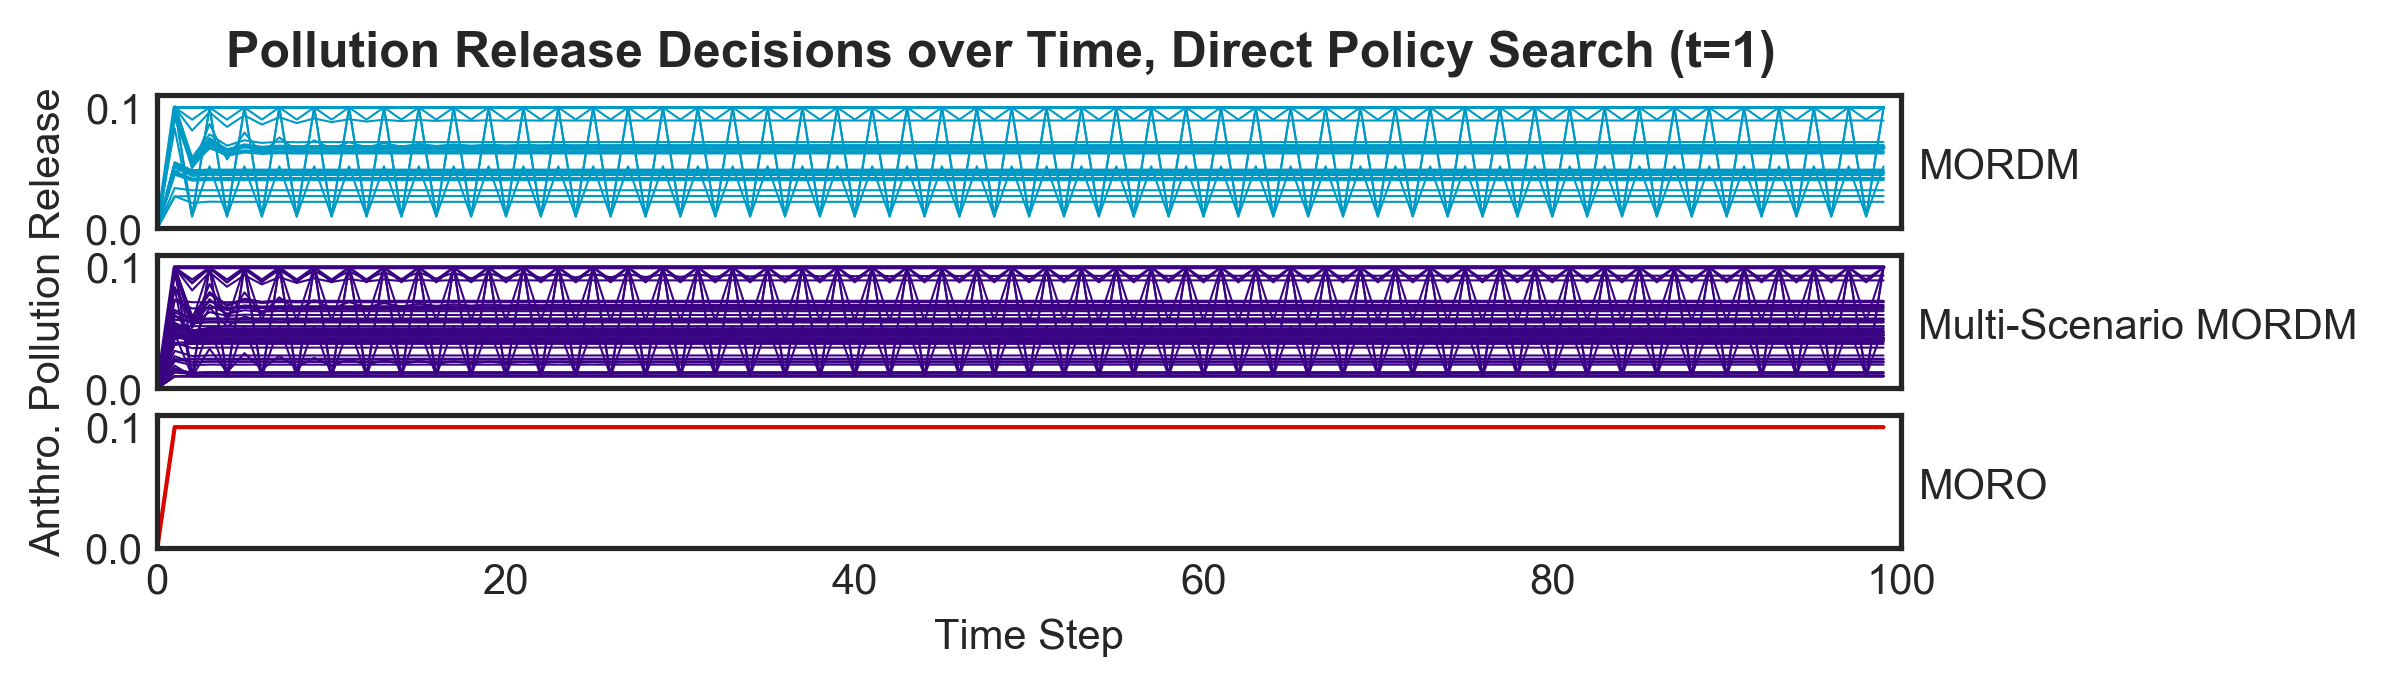
\includegraphics[width=\textwidth]{compare/overtime_dps_highres}
            \label{fig:dps-overtime}
        \end{subfigure}
        
        \caption[Trends in pollution release over time for all pairings]{Trends in pollution release over time of each policy alternative for each model variation and method pairing, assuming base reference scenario uncertainty settings and a starting pollution level of 0.}
        \label{fig:pollution-release-overtime}
    \end{figure}

    The more conservative approach may be driven by the nature of the planned adaptive DPS lake problem, which does not allow for as responsive of decision making as the DPS variation, which can adjust the release amount at every time step, or the intertemporal lake problem, which can also have different release amounts every time period. The anthropogenic pollution release amount over time for identified policy alternatives, shown in \cref{fig:pollution-release-overtime}, as well as the inertia-based robustness values, support this conclusion. The pollution release levels for the planned adapitve DPS lake problem always reach a steady release level, and do so quite quickly, while the other to variations involve frequently changing pollution release amounts over time.

    This trend may also be due to the reference scenarios that were selected for the multi-scenario search phase of the planned adaptive DPS lake problem. To test this theory, a random set of policy alternatives were generated, which were then used in a new multi-scenario MORDM analysis. This lead to a group of policy alternatives, with the mean robustness after uncertainty analysis shown in \cref{fig:robust-heatmap-planned-random}. Comparing robustness values of a random set of reference scenarios to the values generated using the primary set of scenarios generated following the process described in \cref{step2-scenarios} indicates that the selection of reference scenarios has a significant impact on the robustness of policy alternatives. Also, the fact that a random selection of reference scenarios produced robustness similar to MORDM results suggests that the spike in robustness for pollution and reliability (and corresponding drop in utility robustness) is primarily associated with the reference scenario selection and not with any characteristics of the model variation itself. 
    
    \begin{figure}[H]
        \centering
        \captionsetup{width=0.85\textwidth}
        
        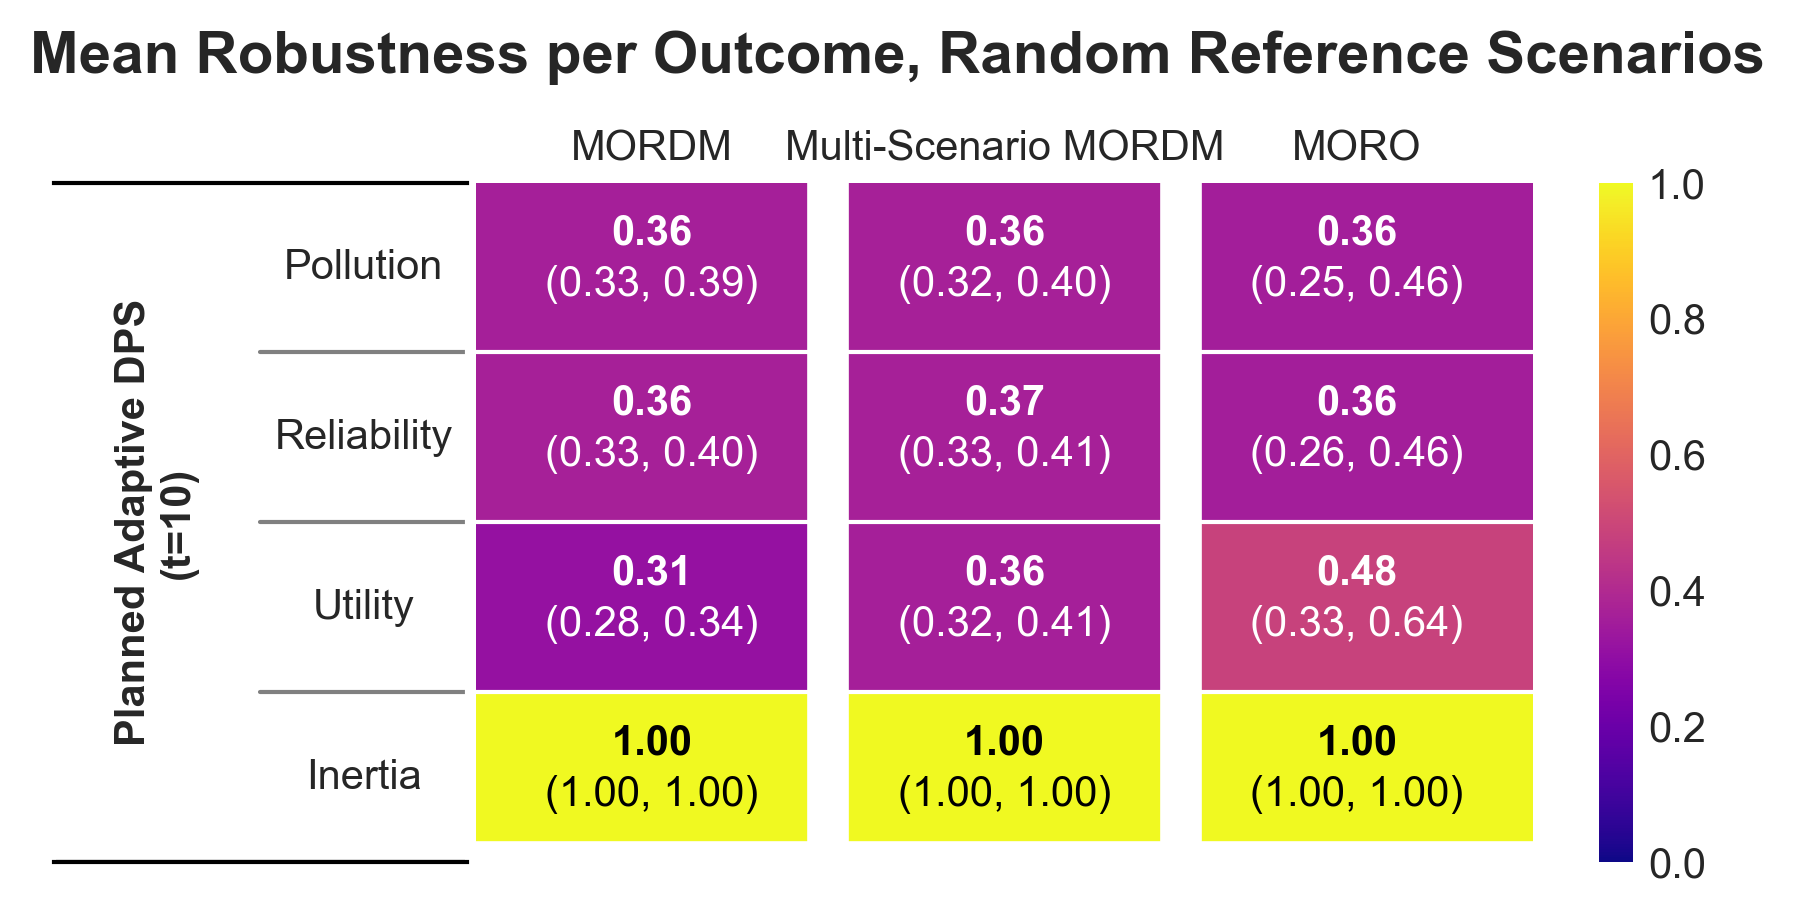
\includegraphics[width=0.85\textwidth]{compare/robust_heatmap_plannedrandom}
        \caption[Mean robustness for planned adaptive variation given random reference scenario selection]{Mean robustness for the planned adaptive DPS problem variation, where multi-scenario MORDM involves the use of a random set of 5 policies.}
        \label{fig:robust-heatmap-planned-random}
    \end{figure}

    \begin{figure}[H]
        \centering
        \captionsetup{width=\textwidth}
        
        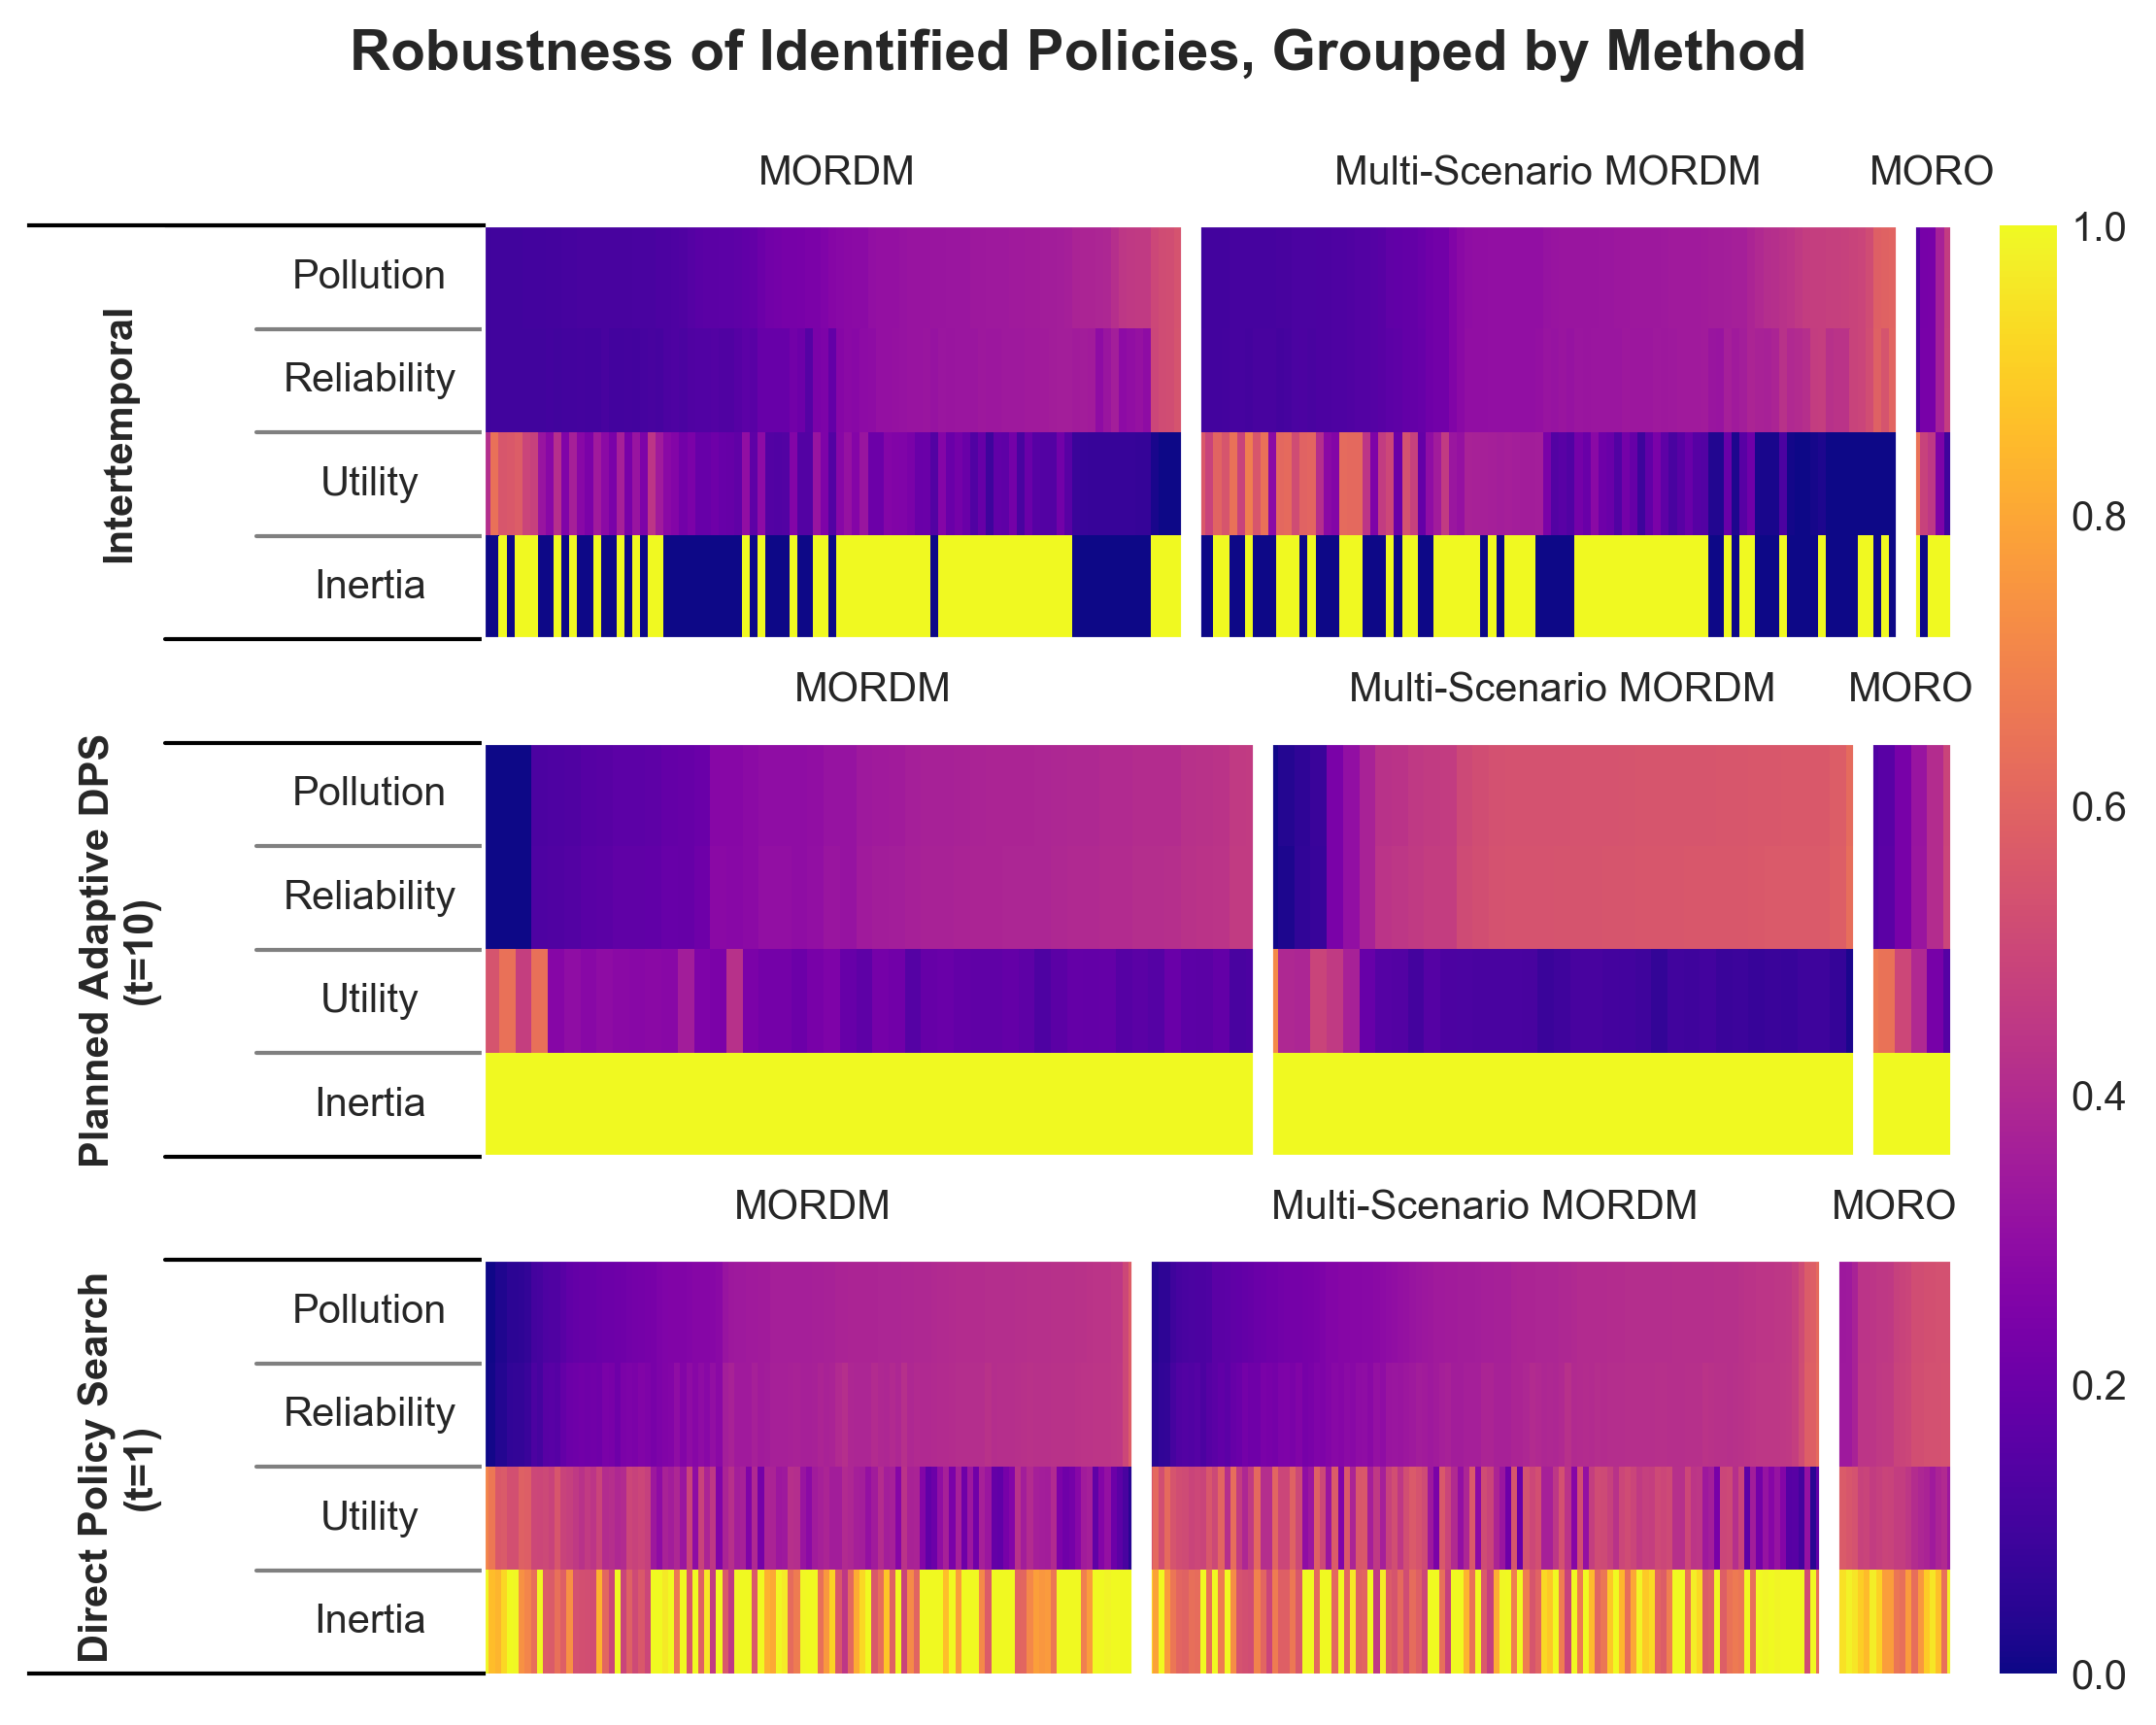
\includegraphics[width=\textwidth]{compare/perpolicyrobustness}
        \caption{Robustness of each outcome of interest per policy in a non-dominated set of alternatives.}
        \label{fig:perpolicy-robustness}
    \end{figure}

    \begin{figure}[H]
        \centering
        \captionsetup{width=\textwidth}
        
        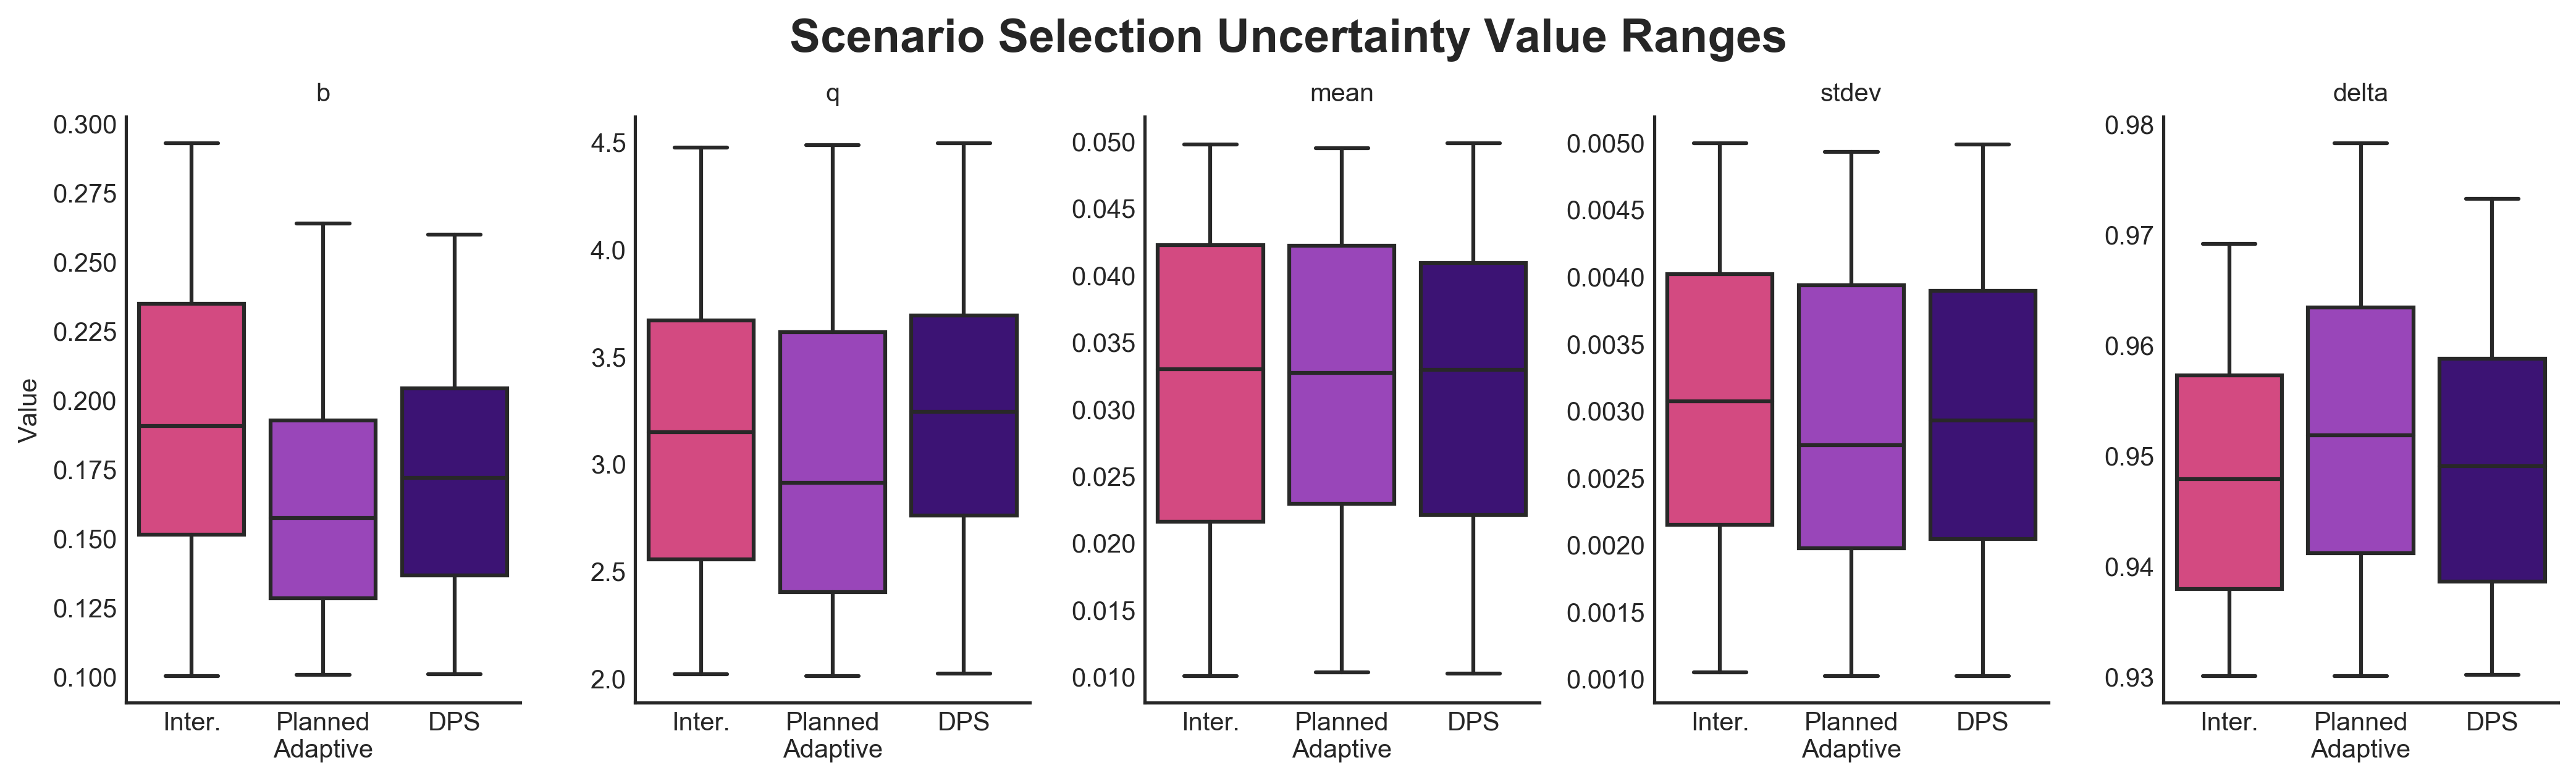
\includegraphics[width=\textwidth]{compare/leverranges_box_scens_highres}
        \caption[Uncertainty value ranges used to select reference scenarios for multi-scenario MORDM]{Ranges of values for each uncertainty parameter that is used to determine a maximally diverse set of 4 policies in the scenario selection process for multi-scenario MORDM.}
        \label{fig:scenarioselect-ranges}
    \end{figure}

    \cref{fig:scenarioselect-ranges} shows the value ranges of each uncertainty parameter that exists in the ensembles of uncertainty vectors that were used to build the sets of 4 maximally diverse policy alternatives for each of the three model variations. This shows that despite the set of reference scenarios for the planned adaptive DPS model variation leading to a set of quite conservative polices, those reference scenarios were selected from a larger ensemble with a relatively similar range of values to the intertemporal and DPS variations. This figure together with the results of the multi-scenario MORDM analysis of the different model variations may indicate that a multi-scenario MORDM analysis of a problem with a policy architecture similar to the planned adaptive DPS, which does not adapt as quickly is more strongly influenced by the reference scenarios selected than the other variations which do. 
    
    The existence of conservative policies with respect to pollution level, which also appears to negatively impacts utility-based robustness, also seems to have had an impact on the diversity of robust outcomes, which provides decision makers with less room for examining the trade-offs that exist when considering a problem with conflicting objectives. As \cref{fig:perpolicy-robustness} indicates, the multi-scenario MORDM analysis of the planned adaptive DPS lake problem does not offer as many policy alternatives that have higher utility robustness and lower pollution and reliability robustness when compared to every other pairing. 

    Also of note in \cref{fig:robust-heatmap-mean} with respect to the planned adaptive DPS model variation is that an increase in robustness of pollution and reliability is not seen in the MORO-based analysis with respect to the MORDM-based analysis, which contrasts with the intertemporal and DPS model variations. This is paired with an increase in robustness of utility for the town, which indicates that while the MORO-based analysis was not able to discover policies that yield a more robust policy with respect to pollution release, it was able to discover policies that maintain a similar level of robustness there while at the same time increasing utility to the town. 
    
    \begin{comparisonbox}{Summary: Robustness of recommended policy set}
        In general, the recommended policy set yielded more robust alternatives the more robustness was incorporated into the search phase of a method, with MORDM yielding the least robust options and MORO the most robust. The exception to this finding is with a multi-scenario MORDM analysis of the planned adaptive model variation. In this case, the policies identified were much more conservative and therefore robust with respect to pollution release and reliability, leading to lower effectiveness for the utility of the town. 
    \end{comparisonbox}
    
    \subsection{Comparison \thecomparison : Similarity of recommended policy sets} \stepcounter{comparison}
    Similarity is examined within method-generated sets of non-dominated policies and is defined as described in \cref{compare-policysimilarity}. The distribution of similarity values for both options, where each value represents the Euclidean distance between two policy alternatives, can be found in \cref{fig:lever-similarity}. 

    \begin{figure}[ht]
        \centering
        \captionsetup{width=0.9\textwidth}

        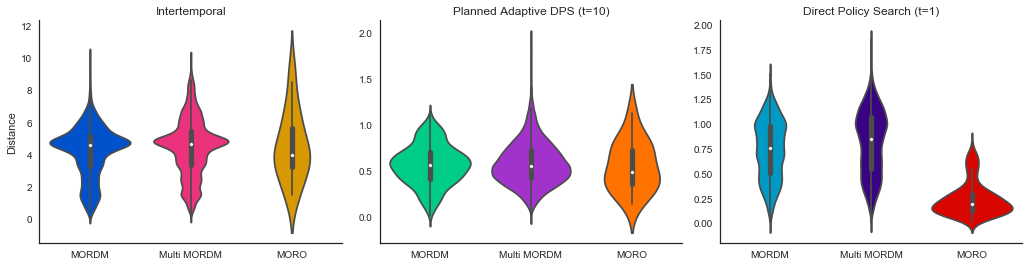
\includegraphics[width=\textwidth]{compare/lever_similarity_within}
        
        \caption{Similarity of lever values, determined between policies of the same method.}
        \label{fig:lever-similarity}
    \end{figure}
    
    \begin{figure}[ht]
        \centering
        \captionsetup{width=\textwidth}
        
        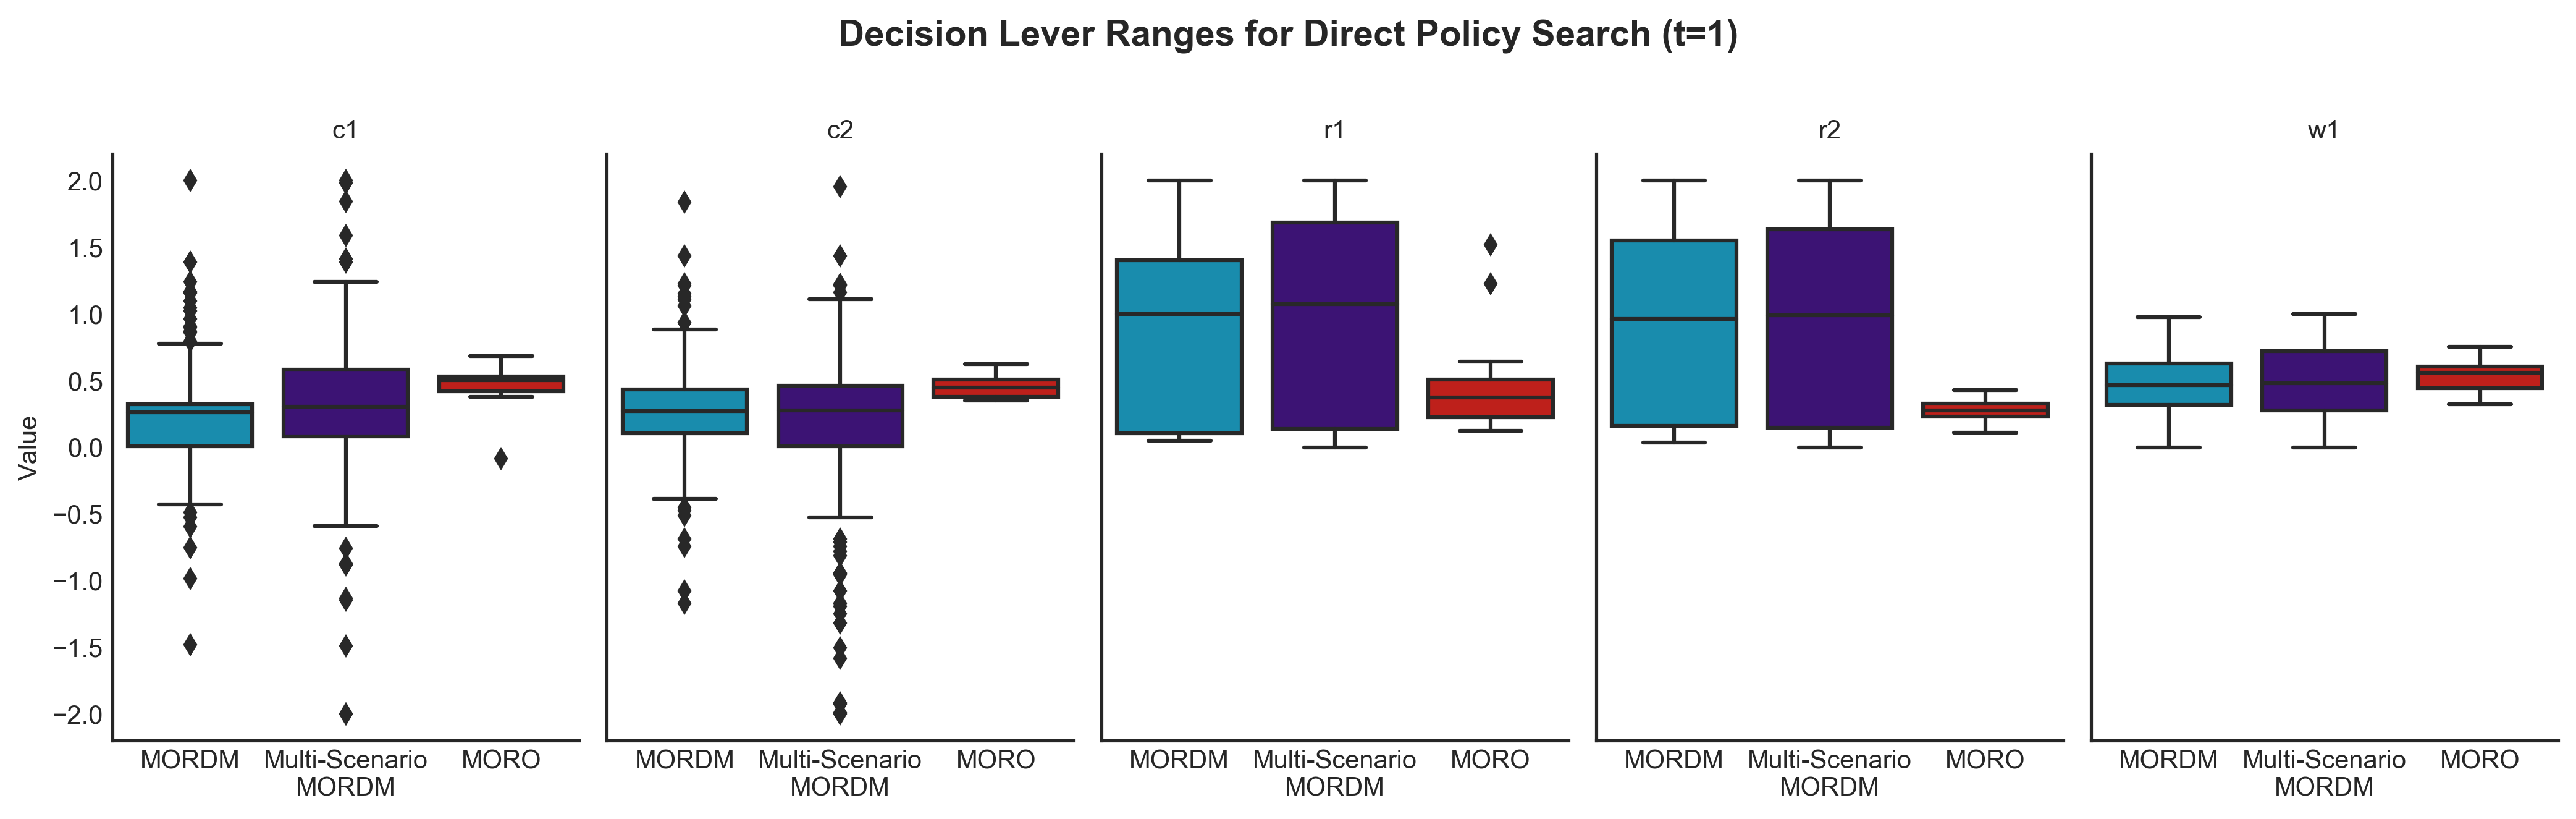
\includegraphics[width=\textwidth]{compare/leverranges_box_dps_highres}
        \caption{Ranges of values for each lever in the non-dominated policy set for the DPS model variation.}
        \label{fig:dps-lever-variation}
    \end{figure}

    \cref{fig:lever-similarity} shows the similarity of sets of policy alternatives to other policies in the same set. A smaller mean distance value, indicated by the white dot in each violin plot element. This chart indicates that there is fairly consistent similarity of policy alternatives within the intertemporal and planned adaptive DPS problem variations. A note within the pairing of the planned adaptive DPS variation and multi-scenario MORDM is the long tail on the upper part of the plot. This indicates that the multi-scenario MORDM method uncovered a small number of policies that are less similar than other policies in the set, given the larger distance value.

    There is an indication that the set of non-dominated policy alternatives generated for the DPS lake problem through MORO results in a less diverse policy set, due to the significantly smaller mean distance values shown in \cref{fig:lever-similarity}. This indicates that decision makers will have a less diverse set of options to work with, which may prove problematic as decision makers seek to balance conflicting objectives. This is born out in \cref{fig:dps-lever-variation}, which shows the ranges of values for each decision lever for the DPS model variation found with each method. With this plot, it is clear that the MORO analysis produces polices from a smaller range of values for each decision lever. At the same time, as seen in \cref{fig:robust-heatmap-mean}, a greater robustness was achieved for each of the outcomes of interest for the DPS + MORO pairing, indicating that despite MORO uncovering a less diverse set of policy alternatives, that set of alternatives is more robust overall, providing a stronger set of alternatives to decision makers for further analysis and development. 
    
    \begin{comparisonbox}{Summary: Similarity of recommended policy sets}
        Save a two identified exceptions, each method is produces sets of policy alternatives with fairly consistent similarity. The multi-scenario MORDM analysis of the planned adaptive DPS variation produces a small number of outlier policies that are less similar than the large majority of policies in that set. Finally, the MORO analysis of the DPS problem variation produces a significantly less diverse set of alternatives, but that set of alternatives is still able to produce a higher level of robustness than is found with the other two methods. 
    \end{comparisonbox}
    
    \subsection{Comparison \thecomparison : Similarity of robustness values} \stepcounter{comparison}
    The final point of comparison considers the similarity of robustness values given a set of similar policies. The purpose of this metric is to determine how robustness is reported for similar policies, to establish a better frame of reference for comparing robustness values of the different methods being studied. In the case of this research, the robustness measure is defined in an identical manner for all three methods. Therefore, the robustness values are directly comparable across method and model parings, and identical policies identified with different methods and tested against the same ensemble of uncertainty vectors in the computational exploration phase will result in identical robustness values. 
    
     \begin{comparisonbox}{Summary: Convergence of search}
        Because all three methods under consideration use the same robustness metric and share a common parameterization of that metric, robustness values will be the same for identical policies found with different methods. 
    \end{comparisonbox}
        

\part{Discussion} \label{part-discussion}
\chapter{Conclusions and Recommendations}
\label{chapter-conclusion}

\begin{abstract}
This study has, until now, involved three phases: 1) A review and development of key concepts, 2) A guide to the specification of three key robust decision support methods and three variations of the highly stylized lake problem, and 3) a conversation about the results of each method and model pairing and a comparison between pairings. In the first part of this final stage of the IMRAD structure, the key developments of this study will be discussed. Information from the first stages of this study will then be leveraged to answer the primary research question. 

\begin{researchquestion}{Research Question}
    What are the trade-offs between different methods of decision support when considering a wicked problems and varying policy implementation structures?
\end{researchquestion}

\end{abstract}

\newpage

\section{Process and Developments}
This first section will address the sub-questions that were developed in support of the primary research question in the original research definition. The structure of this section will follow that of the identified sub-questions, found in \cref{def-supporting-questions}. Each sub-question will be repeated as it is discussed for ease of reference. 

    \subsection{Key concepts}
    The first set of sub-questions identified in the research definition are addressed as key concepts in \cref{chapter-review} and are answered below. 
        
        \subsubsection{Robustness}
        \textit{How is robustness defined in policy analysis? }
        
        Robustness has been used in system and policy analysis as an alternative to address existing problems with a search for the optimal solution: the difficulties of precisely defining a model of the system under consideration and of balancing conflicting objectives, and the potential for catastrophic failure if the conditions required for an optimal solution are not maintained. A robust policy has been defined as one that performs well across a variety of possible future states of a system, due to both internal and external changes.
        
        A review of previous uses of robustness in policy analysis revealed a large variety of mechanisms that can be used to measure a policy's robustness. Selection of an appropriate robustness metric is a choice that decision makers and anlysts must make together, based on their threshold for risk and guided by the data provided by an analysis to assess robustness. 
        
        \subsubsection{Robust decision support methods}
        \textit{What are the origins of each of the selected robust decision support methods?}
        
        Through a review of previous literature on optimization and decision making under conditions of deep uncertainty, a generalized structure for a robust decision support framework was developed. The robust decision support methodology as described in this research originated as the robust decision making (RDM) method, which provided way to analyze wicked problems that are deeply uncertain in a structured manner. This early framework provided clear mechanisms for model specification, computational experimentation, and scenario discovery, but did not provide much guidance for specifying policy alternatives that properly balance conflicting objectives. Given that wicked and deeply uncertain problems will always include disagreements among involved decision makers and conflicting objectives, establishing a list of policy alternatives that will provide the highest potential for system robustness and balance the requirements of those conflicting objectives can be extremely difficult. 
        
        To address this gap in RDM, an extension was developed known as MORDM. This was one of the first commonly applied instances of the integration of a multi-objective search for policy alternatives into decision support analysis. The search in MORDM selects policy alternatives based on performance in a single reference scenario. Other extensions of the RDM framework have built on the work of MORDM and attempt to incorporate robustness more and more directly into the multi-objective search. Multi-scenario MORDM does this by using multiple independent reference scenarios across multiple repetitions of the multi-objective search to provide a more diverse mechanism with which to evaluate performance of a policy alternative. MORO, developed into a robust decision support framework in this study, goes even farther by evaluating policy alternatives based on their robustness over a small set of policies. 
        
        These three frameworks are based on the fundamental RDM structure and all use a multi-objective search for policy alternatives. Visual descriptions of the three methods are shown in \cref{fig:diff-flows-conclusion} and provide a clear communication of how each uses and customizes the RDM structure. 
                
        \begin{figure}[h]
            \centering
            \captionsetup{justification=centering}
            
            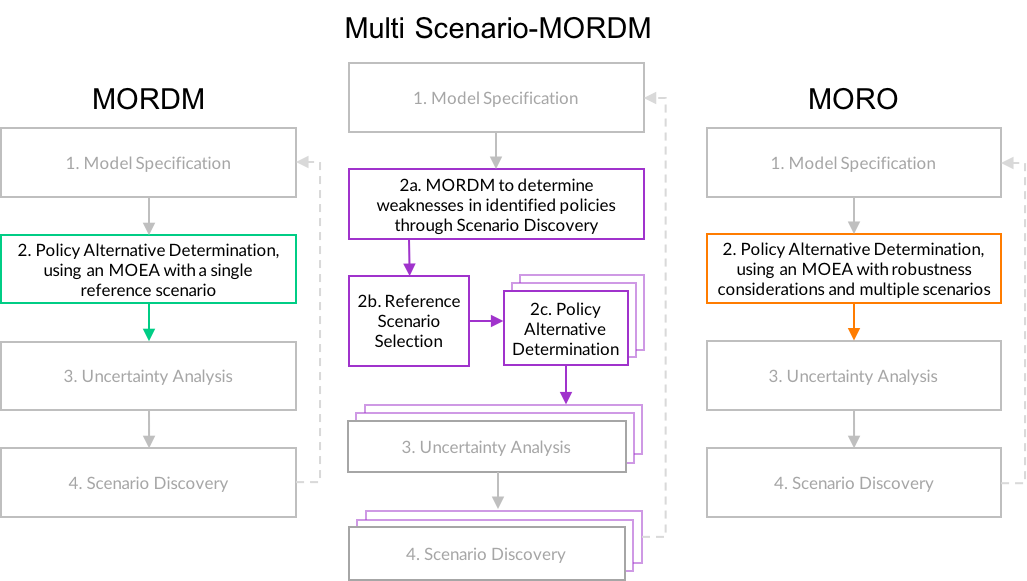
\includegraphics[width=\textwidth]{diff-flows}
            \caption{Comparison of robust decision support framework structures}
            \label{fig:diff-flows-conclusion}
        \end{figure}
    
        \cref{fig:diff-flows-conclusion} highlights the large similarities held by each of the three methods. In fact, steps 1, 3, and 4 are common for all three methods. The difference in methods exists only in step 2: policy alternative determination. And in this step, as described in \cref{dev-step2}, each method uses the same basic multi-objective search algorithm and instantiation of that algorithm, with the differences being concentrated in the mechanism the algorithm uses to compare policy alternatives. By limiting methodological differences to such a small piece of each method, any differences uncovered in this study will be more easily attributable to that single point of difference, providing a stronger foundation for comparison. 
                
        \subsubsection{Evaluating RDM frameworks}
        \textit{How have stylized policy problems been leveraged in previous research?} \newline
        \textit{How does the lake problem incorporate deep uncertainty tipping point behavior?}
        
        To evaluate the performance of each RDM framework against wicked problems with tipping point characteristics, a commonly used stylized problem will be employed: the lake problem. As problems that involve a tipping point generally contain high levels of uncertainty, a point of no return, and conflicting objectives, they are recognized as strong candidates to evaluate decision support frameworks \citep{Ward2015}. The lake problem is a classic tipping point problem that has been used frequently to develop and evaluate robust decision support frameworks \citep{Carpenter1999, Lempert2007, Quinn2017, Singh2015, Ward2015}. The lake problem revolves around a fictional town that is seeking to maximize economic productivity of industry and agriculture through the release of pollution, while at the same time to minimize risk of over-pollution of a nearby lake, represented as a series of four conflicting objectives. 
        
        \textit{What policy implementation structures are commonly recognized in literature?}
        
        Two different variations of the lake problem have been previously developed that represent extremes of static and adaptive policy structures. The intertemporal variation requires policies to use a set of predetermined decisions that define the pollution release level at every time step \citep{Ward2015}. And the direct policy search variation uses decision levers to build a release function that incorporates current pollution levels and is used to set the pollution release level every time step \citep{Quinn2017}. 
        
        Both the intertemporal and DPS policy structures include the ability to alter the amount of anthropogenic pollution release in every time step, which does not reflect typical real world conditions, where such a change often requires significant investment and decision making moves more slowly. A planned adaptive DPS variation of the lake problem was proposed that follows the policy implementation structure of the DPS variation, but updates the release amount every 10 time steps to more accurately reflect policy structure that is found in real world decision making. 
    
    \subsection{Methodology}
    Similar to the key concepts, the next section will address the methodological sub-questions developed as a part of the research definition. The methodology applied in this study was developed in \cref{part-develop}. 
        
        \subsubsection{Lake Problem Variations}
        \textit{What are definitions of the lake problem that represent the three essential types of policy implementation?}
        
        The intertemporal and DPS variations of the lake problem were implemented following the details of previous applications in literature \citep{Kwakkel2017, Quinn2017, Singh2015, Ward2015}. The proposed planned adaptive DPS variation follows the implementation structure of the DPS lake problem, but only refreshes the pollution release amount every 10 time steps instead of at every time step, as is done in the traditional DPS variation. No changes to any of the model variations were required across all three methods of analysis. This, again, limits the differences being considered and ensures a more fair comparison. 
        
        \subsubsection{Method Implementation}
        \textit{How can robustness be determined for each selected robust decision support method?} 
        
        A common robustness definition was used for all three robust decision support methods: Starr's domain criterion \citep{Starr1963}. The exact implementation of this metric was described in \cref{dev-step0}, including a definition of the outcomes of interest and threshold values that are based on previous applications of the lake problem \citep{Quinn2017, Ward2015}. Using a common robustness definition minimizes the differences between method and model variation pairings and allows for a straightforward comparison of results between the three robust decision support methods. 
        
        \textit{What are the implementation details for each robust decision support method identified for this study?}
        
        Further details of each method implementation are found in \cref{dev-step2}. Most notably, an auto-adaptive variation of the $\epsilon$-NSGAII algorithm was developed that combines an epsilon-based multi-objective search using techniques developed by \citet{Deb2002} with auto-adaptive operator selection introduced by \citet{HadkaReed2013} and previously used in the Borg framework. This auto-adaptive $\epsilon$-NSGAII algorithm aims to combine the strongest points of $\epsilon$-NSGAII, a generational MOEA with epsilon dominance, and Borg, which supports auto-adaptive operator selection and auto-adaptive population sizing, to allow for a more rapid convergence to a stable set of non-dominated policy alternatives. The same auto-adaptive $\epsilon$-NSGAII algorithm is used for all three methods in this study, with a common parameterization. The only difference lies in the mechanism used to compare potential policy alternatives during the search process, with each method using their own unique mechanism. These mechanisms were described in \cref{step2-scenarios} and are summarized in \cref{table:conclusion-searchevaluation}. The inclusion of robustness provides a indication of how much robustness was included in the search phase for each method relative to the other methods considered. It is by no means an absolute indication of the inclusion of robustness for each method. 
        
        \begin{table}[H]
            \centering
            \captionsetup{width=\textwidth}
            \caption{Policy alternative comparison mechanism used in the MOEA-based search for each method.}
            \label{table:conclusion-searchevaluation}
            
            \setlength\arrayrulewidth{1pt}\arrayrulecolor{white}
            \rowcolors{2}{odd-row-blue}{even-row-blue}
            \begin{tabularx}{\textwidth}{|l|X|l|}
                \rowcolor{tudelft-dark-blue!80}
                {\color{white} Method} &  {\color{white} Comparison Mechanism} & {\color{white} Inclusion of Robustness} \\ \hline
                
                MORDM & Absolute performance in single base reference scenario & Low \\ \hline
                Multi-Scenario MORDM & Absolute performance in one of a set of reference scenarios, with search repeated for each scenario & Medium \\ \hline
                MORO & Robustness score calculated using a small set of (50) scenarios & High \\ \hline
            \end{tabularx}
        \end{table}
        
        Details of the comparison mechanism for MORDM are quite straightforward, using a single base reference scenario. The multi-scenario MORDM method requires a clear definition of how the set of reference scenarios used is determined. In this case, a set of four scenarios are selected that are maximally diverse within vulnerable ranges identified in MORDM's scenario discovery step. Finally, the MORO method involved defining a constant set of 50 scenarios with which to test each possible policy alternative. Alternatives are then added to the non-dominated set of policy alternatives based on the robustness of each outcome of interest. Robustness is calculated using the established domain criterion metric and thresholds from \cref{dev-step0}. 
        
        In addition to the details established for each method's policy alternative determination step, \cref{dev-step3} and \cref{dev-step4} defined mechanisms for uncertainty analysis and scenario discovery that are shared across all three robust decision support methods and follow the implementation established when the MORDM method was introduced \citep{Kasprzyk2013}. 
        
        \subsubsection{Comparison Specification}
        \textit{What are the points of comparison which should be considered during analysis?}
        
        Existing literature that compare methods for policy analysis were examined to develop a comprehensive set of 11 comparison metrics. This set of metrics serves two purposes. First, to provide a strong and common foundation for future comparisons of policy analysis methods. Second, to establish the metrics with which to compare the three robust decision support methods considered in this study. These metrics include both qualitative and quantitative measures and were divided into three categories: setup complexity, communication, and results. Metrics include complexity of problem and method setup, ease of results communication and response to change, computational cost, robustness of policies, and similarity of results and robustness. Details of each metric are discussed in \cref{dev-comparisons}. 
                
    \subsection{Results}
    The final group of sub-questions address the results of each method and model variation pairing, along with the comparisons made. A detailed analysis of the results was included as \cref{part-analysis}. 
    
        \subsubsection{Individual Results}
        \textit{What are the results from each pairing of robust decision support method and variation of the stylized policy problem?}
        
        Considering the results of each method variation and method pairing separately provides the foundation for a comparative analysis by establishing the validity of each pairing before attempting any direct comparisons. These individual results were discussed in \cref{analysis-results}. The results showed that the MOEA search for each pairing stabilized successfully to a promising set of policy alternatives. The uncertainty and scenario discovery results were also summarized in \cref{analysis-results}. 
        
        %TODO EEB compare results to existing analysis (Quinn, Wade, etc. )
        
        \subsubsection{Comparison of Results}
        \textit{Based on the points of comparison defined in \cref{dev-comparisons}, how do the results of each pairing compare?}
        
        After the individual results were examined and validated, a comparison was made. Using the metrics defined in \cref{dev-comparisons}, \cref{chapter-comparison} compared the various method and model variation pairings. This section summarizes the key findings made during comparison and is divided into three categories, following the structure established with the comparison framework in \cref{dev-comparisons}. 
        
        \textbf{Setup} \newline
        With respect to problem complexity, each method is able to use the same implementation of each lake problem variation, so there is no difference in setup. 
        
        Method setup complexity includes some variable differences. Given the method implementations used for this study, the setup of multi-scenario MORDM requires a complete MORDM analysis and extensive additional computation to determine a maximally diverse set of reference scenarios, so setup is significantly more complicated than it is for the other two methods. It is important to note that the complexity of setup for multi-scenario MORDM can be reduced by using a different mechanism to build the set of reference scenarios than is used in this study.
        
        \textbf{Communication} \newline
        Each method is able to use the same definition of robustness and builds final results with the same processes of policy alternative determination, uncertainty analysis, and scenario discovery, so there is no difference in the communication of results or robustness for this study. 
        
        The common implementations for the final two steps in the RDM flow also mean that there is no significant difference in the updating the results of those two stages if the model or robustness metric changes. One exception lies in the impact of a change in robustness metric to the policy alternative determination process for MORO-based analyses. Because MORO directly integrates robustness into the search process, an update to the metric will require a restart of the policy alternative determination process. 
        
        \textbf{Results} \newline
        MORO requires significantly higher computational cost, given that each potentially promising policy alternative must be evaluated over 50 scenarios and not just one. With that cost, though, comes a generally smaller and more robust set of non-dominated alternatives than what is found with the other two methods. The robustness of each set of non-dominated policy alternatives indicate that the more robust considerations are incorporated into the search process, the higher the robustness of the final non-dominated set of alternatives will be. This is seen in the heatmap of mean robustness values for each method and model variation pairing that was included in \cref{results-compare-results} and is reproduced here as \cref{fig:conclusion-robust-heatmap-mean} for ease of reference.
        
        The exception to the general rule of increasing robustness can be seen with the results of the planned adaptive DPS model variation. A sharp increase in robustness with respect to pollution level and reliability was found in the multi-scenario MORDM analysis of the planned adaptive DPS variation that was not seen with the other two variations. A likely cause lies in the set of recommended policies for that pairing, which were much more conservative with respect to the amount of pollution released in each time step. The set of non-dominated policies for this pairing were also found to lead to a less diverse set of robustness outcomes, with most of the policies yielding high robustness with respect to pollution and reliability and lower robustness with respect to utility (as displayed in \cref{fig:perpolicy-robustness}).
        
        These facts together demonstrate the significant impact that the reference scenario selection process can have during a multi-scenario MORDM analysis, which can lead to results that prioritize one outcome of interest over another. Because it is impossible for problems characterized by deep uncertainty to include a consistent ranking of the preference of outcomes of interest, such a prioritization of one outcome in the policy alternative determination process should be avoided wherever possible.
        
        Additional study of the planned adaptive DPS model variation and multi-scenario MORDM pairing was completed that compared the results of the reference scenario selection method applied in this study with a random scenario selection. Robustness results using random scenario selection produced values similar to what was found with the traditional MORDM analysis, which adds emphasis to the importance of reference scenario selection on the analysis process. Given that the same mechanism is used to select reference scenarios for all three problem variations, there are also indications that the slower moving policy structure found in the planned adaptive DPS variation is more susceptible to strong influences from the selection of reference scenarios. 
      
        \begin{figure}[H]
            \centering
            \captionsetup{width=0.8\textwidth}
            
            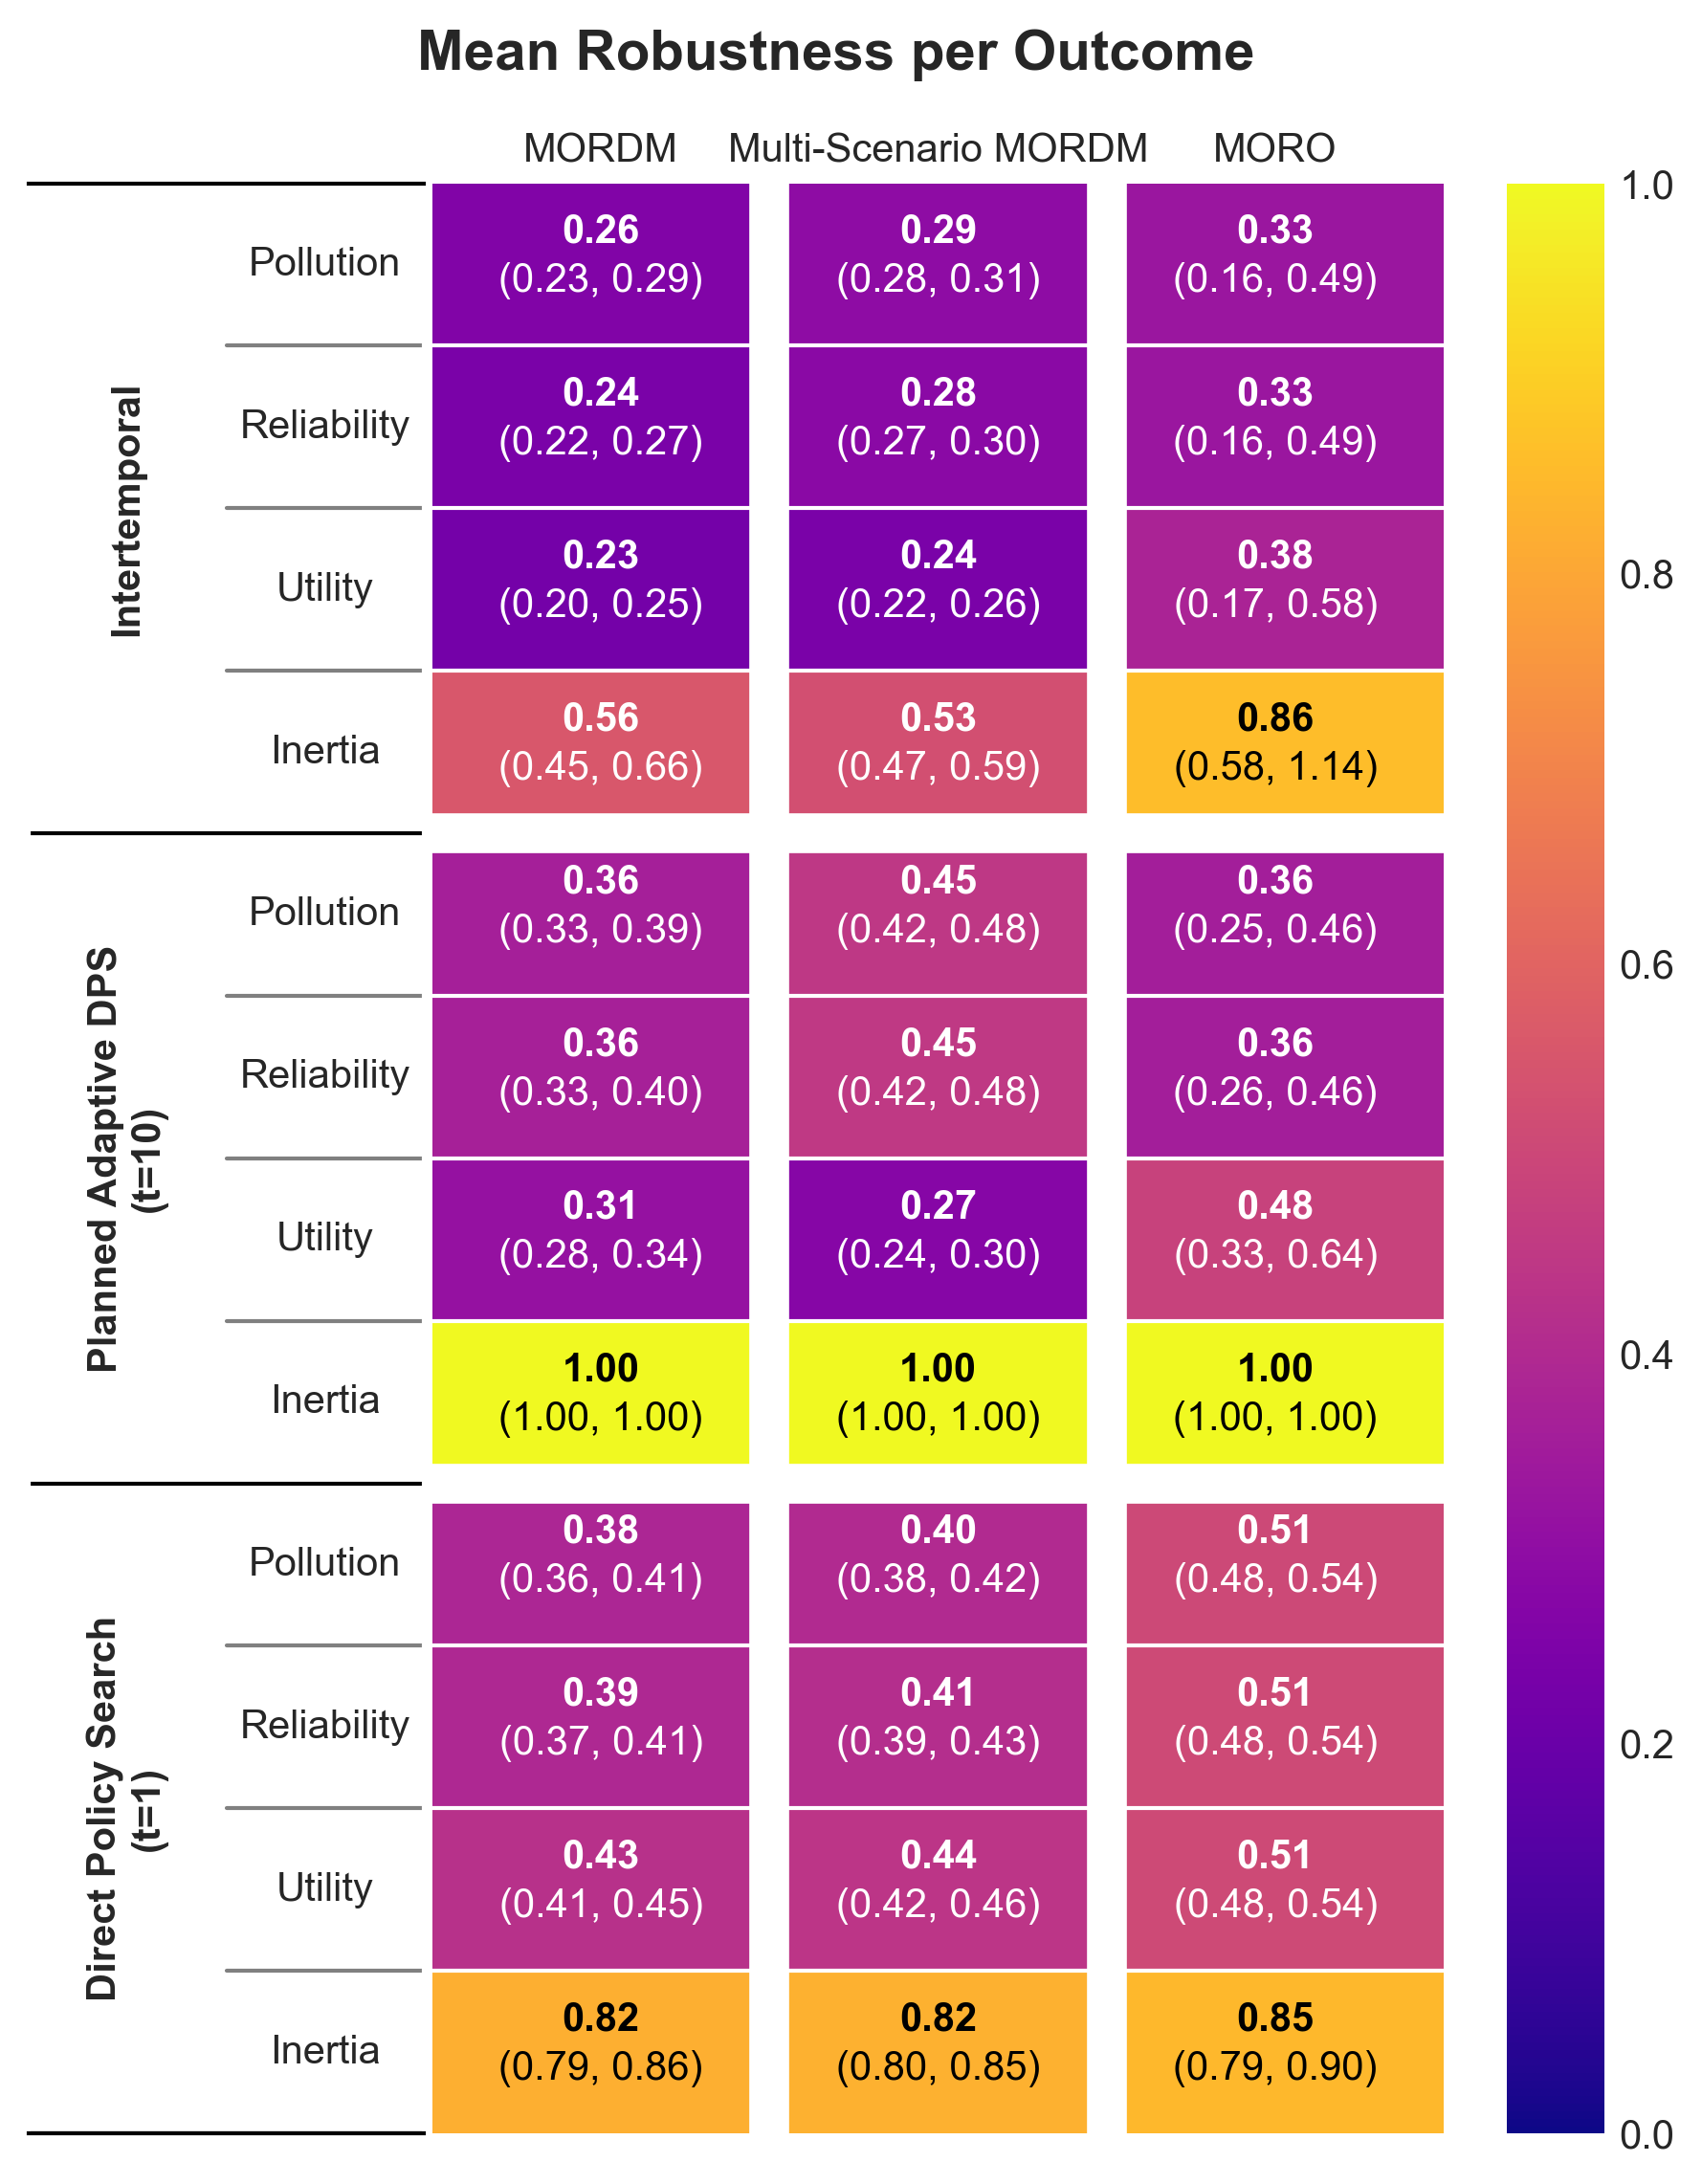
\includegraphics[width=0.8\textwidth]{compare/robust_heatmap_mean}
            \caption[Mean robustness per outcome of interest across all pairings]{Mean robustness per model variation and method pairing. This heat map is annotated to include the bounds of the 95 percent confidence interval surrounding the mean.}
            \label{fig:conclusion-robust-heatmap-mean}
        \end{figure}
              
\section{Answering the Primary Research Question}
The answers to each sub-question can now be used to answer the primary research question, repeated here. 

\begin{researchquestion}{Research Question}
    What are the trade-offs between different methods of decision support when considering a wicked problems and varying policy implementation structures? 
\end{researchquestion}

The categorization of each point of comparison considered in this analysis provide a structure for considering trade-offs that exist when determining which robust decision support method to use in an analysis of a wicked policy problem with tipping point characteristics. In this study, the first category, setup complexity, provides little guidance to distinguish the three methods, as each was executed using the same software tooling and has the same requirements for model implementation. Of course, as discussed in \cref{dev-step0}, there are other packages that support the policy analysis process as well that are not able to support all three analysis methods. In that case, there may be significant differences in the setup complexity for both the model and method being used. 

The second category, communication and interaction, provides some stronger trade-offs between methods. The MORDM method is least affected by changes in model or robustness specification. A change in robustness metrics during an MORDM-based analysis would only require recalculation of the robustness values of each policy alternative using an already completed ensemble of computational experiments. A change in robustness metric configuration may require a restart of part, in the case of multi-scenario MORDM, or all, in the case of MORO and multi-scenario MORDM, of the policy alternative determination process. Therefore, if the configuration of a robustness metric is more likely to change during the course of an analysis, decision makers may be more interested in an MORDM-based analysis. 

The final category of comparison metrics provides the most opportunity for differentiation between methods. As indicated by \cref{table:conclusion-computational-cost}, a MORO analysis has a significantly higher computational cost than for the other robust decision support methods. The increased computational cost had a significant impact on the time it took to complete the analysis even for a highly-stylized and relatively low computational cost problem like the lake problem used in this analysis and can have an even more significant impact when considering policy problems that require significantly more complex models with more sources of uncertainty than are present in the lake problem. 

\begin{table}[b!]
    \captionsetup{width=0.99\textwidth}
    \caption[Computational cost across all pairings]{Computational cost of the MOEA-based search determined for each model variation and method pairing. Total computational cost, calculated as number of model function executions, can be found in the last row.}
    \label{table:conclusion-computational-cost}
    
    \rowcolors{2}{odd-row-blue}{even-row-blue}
    \setlength\arrayrulewidth{1pt}\arrayrulecolor{white}
    \begin{tabularx}{0.99\linewidth}{l|l|R|R|R}
        \hline
        \rowcolor{tudelft-dark-blue!80}
        \multicolumn{2}{l|}{\color{white} \textbf{}} 
        & \multicolumn{1}{c|}{\color{white} \textbf{MORDM}} 
        & \multicolumn{1}{c|}{\color{white} \textbf{\begin{tabular}[c]{@{}c@{}}Multi-\\ Scenario \\ MORDM\end{tabular}}}
        & \multicolumn{1}{c}{\color{white} \textbf{MORO}} \\ \hline
        
        \cellcolor{even-row-blue}   & Intertemporal    & 500,000   & 500,000  &  300,000    \\ \cline{2-5} 
        \cellcolor{even-row-blue}   & \cellcolor{odd-row-blue}Planned Adaptive &
        \cellcolor{odd-row-blue}100,000   & \cellcolor{odd-row-blue}100,000  & \cellcolor{odd-row-blue}100,000     \\ \cline{2-5} 
        \multirow{-3}{*}{\cellcolor{even-row-blue}\begin{tabular}[c]{@{}l@{}}Number of \\ Function \\ Executions (NFE)\end{tabular}} & DPS             & 100,000   & 100,000  & 100,000      \\ \hline
        
        \multicolumn{2}{l|}{\cellcolor{odd-row-blue}Per Policy Executions} & 1 & 1 & 50 \\ \hline
        \multicolumn{2}{l|}{\cellcolor{even-row-blue}Search Repetitions} & 1 & 5 & 1 \\
        
        \noalign{\global\arrayrulewidth=4pt} \arrayrulecolor{tudelft-dark-blue!80}
        \hline
        \noalign{\global\arrayrulewidth=1pt} \arrayrulecolor{white}
        
        \cellcolor{odd-row-blue}    
        & \textbf{Intertemporal}    & 500,000  & 2,500,000 & 15,000,000  \\ \cline{2-5} 
        \cellcolor{odd-row-blue} 
        & \cellcolor{even-row-blue}\textbf{Planned Adaptive} & \cellcolor{even-row-blue}100,000  & \cellcolor{even-row-blue}500,000   & \cellcolor{even-row-blue}5,000,000    \\ \cline{2-5} 
        \multirow{-3}{*}{\cellcolor{odd-row-blue}\textbf{\begin{tabular}[c]{@{}l@{}}Computational \\ Cost (NFE) \end{tabular}}}      
        & \textbf{DPS}              & 100,000  & 500,000   & 5,000,000           \\ \hline
    \end{tabularx}
\end{table}

Contrasted with computational cost is the robustness of each recommended set of non-dominated policy alternatives. As highlighted earlier in this chapter, the robustness of a non-dominated set of alternatives is generally seen to increase as the consideration of robustness in the search process increases. The trade-off then becomes one between robustness of the recommended set of policy alternatives and computational cost of analysis, where decision makers who are able to sacrifice time and computational cost and who are interested in the most robust options may desire a MORO-based analysis, and decision makers who are unable to spend the additional computational cost may prefer a MORDM-based analysis. A multi-scenario MORDM-based analysis can provide a middle path between the two extremes of MORDM and MORO, but issues of setup complexity and the impact of reference scenario selection may outweigh the benefits of a small amount of added robustness obtained with multi-scenario MORDM.

Also worth consideration is the size of each set of non-dominated policy alternatives, summarized in \cref{table:conclusion-pareto-size}. Both MORDM and multi-scenario MORDM based analyses lead to a significantly larger number of non-dominated policies that must then be considered throughout the remaining steps of analysis. Methods that recommend larger sets of policy alternatives can prove to be more difficult for decision makers to digest in order to reach a final plan of action. 

At the same time, consideration of a larger set of policy alternatives can provide a more diverse set of options for decision makers to chose from, providing more opportunity to determine how best to balance conflicting objectives through discussion and debate after an a priori analysis has been completed with as minimal an influence from decision makers as possible. This represents the final trade-off discussed as a part of this study. Decision makers who are interested in a small set of robust policy options may prefer a MORO-based analysis, while decision makers who are more interested in a large and diverse set of alternatives to consider further may prefer either an MORDM or multi-scenario MORDM-based analysis. 

\begin{table}[h]
    \centering
    \captionsetup{width=0.85\textwidth}
    \caption[Size of non-dominated policy alternative sets]{Size of the Pareto non-dominated set of policy alternatives for each model variation and method pairing.}
    \label{table:conclusion-pareto-size}
    
    \rowcolors{2}{odd-row-blue}{even-row-blue}
    \setlength\arrayrulewidth{1pt}\arrayrulecolor{white}
    \begin{tabularx}{.85\linewidth}{l|R|r|R}
        \rowcolor{tudelft-dark-blue!80}
        & \multicolumn{1}{c|}{\color{white} \textbf{MORDM}}
        & \multicolumn{1}{c|}{\color{white} \textbf{Multi-Scenario MORDM}}
        & \multicolumn{1}{c}{\color{white} \textbf{MORO}} \\ \hline
        
        Intertemporal       & 90    & 291   & 7     \\ \hline
        Planned Adaptive    & 48    & 113   & 6     \\ \hline
        DPS                 & 110   & 209   & 22    \\ \hline
    \end{tabularx}
\end{table}

\chapter{Reflection}
\label{chapter-reflection}

\begin{abstract}
    Given the detailed analysis described throughout this thesis and the conclusions reached, this chapter will discuss the implications of these conclusions. The gaps identified in the introduction will be reviewed and addressed in \cref{reflect-gaps}. The contributions made by this study and their added value to both decision makers and analysts is discussed in \cref{reflect-goals}. Finally a discussion of what the two relevant parties, policy analysts and decision makers, can take away from this study is found in \cref{reflect-application}
\end{abstract}

\newpage

\section{Response to Identified Gaps} \label{reflect-gaps}
In the introduction of this thesis, three different gaps in current research were identified that should be addressed with this research. This section will review those gaps and the progress this study has made toward addressing those gaps. For reference, the identified gap is included at the start of each sub-section. 

    \subsection{Research Gap One}
    \textit{Robust optimization techniques have not yet been integrated into an RDM-based decision support process in literature.}
    
    In the review of concepts, this study developed a common RDM-based structure for the three methods considered. Through that effort, traditional robust optimization techniques were integrated into a method identified as multi-objective robust optimization (MORO). The common structure used for MORO and the other two identified methods of robust decision support (shown in \cref{fig:diff-flows-conclusion}) provide a strong foundation for comparisons made in this study by making the differences and similarities between methods very clear. There are, of course, remaining avenues of research with respect to the development of the MORO method, which are discussed in \cref{chapter-futurework}.
    
    \subsection{Research Gap Two}
    \textit{There is a lack of comparative analysis of the identified robust decision support methods that can help decision-makers determine which method is most suitable to their needs.}
    
    As one of the primary goals of this study was to provide an in-depth comparison of the identified methods of robust decision support, this study does provide an as of yet nonexistent comparison of these methods. Unlike most previous comparison literature, which compare different methods of decision support using an application to a single case and policy structure \citep{Gersonius2016,Hall2012,Roach2015}, this study uses three different policy structures for a single problem to develop a comparison, which provides a broader scope for comparing the methods of interest. 
    
    Also unlike several existing comparisons, this study uses a highly stylized policy problem that is not founded in a real-world wicked problem. Using a commonly referenced and highly stylized policy problem reduces the risk of skewed results due to a biased or poorly implemented model. At the same time, however, a simplified problem like the lake problem may not be able to provide enough complexity to fully test the capabilities of the methods under consideration, which may affect the validity of any conclusions made in a comparison using such a problem. The potential shortcomings held by the lake problem are discussed further in \cref{chapter-futurework}. 
    
    \subsection{Research Gap Three}
    \textit{Existing work that compares decision support methods focuses on one specific case and one policy implementation structure, and not the impact of varying policy structures on the results of analysis.}
    
    This study has introduced the concept of comparing decision support methods using three varying policy formulations by comparing three methods of robust decision support against three variations of the problem identified: the shallow lake problem. Two of the structures used have been commonly referenced in policy analysis literature and represent extreme implementations of both static and adaptive policies \citep{Carpenter1999, Quinn2017, Singh2015, Ward2015}. The intertemporal variation represents a static policy where the level of anthropogenic pollution released at every time step is static and defined through 100 independent decision variables. The direct policy search (DPS) variation represents the other extreme - a highly adaptive policy structure where the amount of pollution to be released is determined for every time step based on a formula that is parameterized using 5 decision levers. 
    
    This research proposed a third and more realistic policy implementation structure: planned adaptive DPS. This variation follows the basic structure of the DPS problem but updates the amount of anthropogenic pollution released every 10 time steps, instead of at every time step. This variation produced results that differed from the DPS and intertemporal variations, especially with respect to the robustness of the non-dominated set of alternatives generated with multi-scenario MORDM. Together, these three problem variations support the comparison of decision support methods against multiple policy variations from the same wicked problem. 
    
    Just like the previous two gaps, there is additional research that can be done regarding the development of policy implementation structures that best reflect real-world conditions of policy making. This, as well, is discussed in further detail in \cref{chapter-futurework}.
    
\section{Contemplating Goals of the Study} \label{reflect-goals}
This thesis began by introducing the concept of a wicked problem and the difficulties associated with attempting to solve wicked problems, especially those that include irreversible tipping point behaviors. As these problems are subject to conditions of deep uncertainty, which cannot be easily described, a new type of analysis is required. Several methods have been developed that, instead of attempting to use a single predictive model and seeking a single optimal solution, seek a series of robust policy alternatives which can inform decision making these methods are identified as robust decision support methods for the purposes of this study. 

Despite the existence of several methods of robust decision support, there remains no clear way for decision makers and analysts to compare methods and determine which is most suitable for each individual wicked problems. Previous literature has completed independent and unique comparisons using many different wicked problems and many different focuses for comparison. This leads to the first contribution that this study is making to the area of policy analysis for wicked problems.

    \subsection{A structured comparison framework}
    This study has developed a systematic framework for comparing many decision support methods. Several points of comparison are included and were developed through in-depth analysis of previous literature that has compared policy analysis methods \citep{Gersonius2016,Hall2012,Matrosov2013a,Roach2015}. These previous studies have used a wide variety of comparison metrics, which have led to conclusions that are less generalizable than a systematic approach may offer. 
    
    The comparison framework developed can be easily extended to compare new methods and new wicked problems, as the points of comparison will cover a broad set of differences between methods and problems. There exist points of comparison that are not relevant for the work done for this study, but may be relevant given different methods or models. This study, therefore, sought to develop a broad set of comparison metrics to ensure that it remains applicable for many other decision support methods. Several visualizations were developed to support these comparison metrics that can also be generalized to new methods and models.
    
    Care must be taken when attempting to compare methods of decision support, though. This study made great efforts to ensure that the differences in methods and problems being compared were kept to a minimum by using common definitions and implementations wherever possible. By doing this, any differences observed can be more easily attributed to the single component of each method that is different, and not to the decision support method in general. When considering new methods, it is important to keep in mind which aspects of each method are being compared, and to limit method variation to just those aspects of each method that are being compared. 
    
    For example, this study in the current form examines the impact of different policy alternative evaluation mechanisms in the MOEA-based search for alternatives. Apart from that variation, the remaining structure and implementation of each method is consistent. This allows the analyst to examine the impact of just that element of a robust decision support method. Alternatively, an analyst may want to examine the impact of different MOEAs altogether. If this is the case, the same method should be used with different MOEAs, keeping the remaining elements consistent (including the policy alternative comparison mechanism within each search algorithm), to more clearly examine the impact of different algorithms on the method itself.
    
    Instructions for extending the comparison completed in this thesis using the method, model, and execution implementations developed for this thesis can be found in \cref{appendix-code}. 
        
    \subsection{A comparison of three robust decision support methods}
    The framework for comparison is then used to compare the results from a series of three methods and three model variations. This is the primary goal sought by the main research question. Applying the comparison framework provides information about how each method handles a wicked problem with different policy implementation structures, and more generally demonstrates how the framework can be applied to other methods and models in the future. 
    
    The first significant contribution as a part of this comparison was the formalization of a common structure for all three methods under consideration, as seen in \cref{fig:diff-flows-conclusion}. This is the first time that the MORO method was formalized to follow the RDM structure, as well as the first time that all three methods are formalized in a common way. This structure provides a foundation for implementing each of the three methods consistently and ensuring that the focus of comparison remains on the variable element of the three methods: the comparison mechanism used in an MOEA-based search.  
    
    Given method implementations that follow the RDM-based structures in \cref{fig:diff-flows-conclusion} and model variations that follow the three identified policy structures from \cref{review-structure}, a structured comparison was made. As a significant portion of the three methods use common implementations, several points of comparison in the framework do not result in any significant conclusions about the trade-offs between methods. 
    
    The comparison framework did identify a couple of key differences. First that the more robustness is incorporated into the search process of a method, the more robust the identified policy alternatives will be. But the incorporation of robustness comes with additional computational costs. MORO, which uses robustness the most in the policy alternative determination step, also has a significantly higher computational cost than the other two methods of analysis. 
    
    The framework also revealed inconsistencies in the results for the planned adaptive DPS variation and multi-scenario MORDM method pairing. This pairing was shown to produce an extremely conservative set of policy alternatives, with respect to maintaining low levels of pollution in the lake. And, as utility is a conflicting outcome of interest, the increase in robustness seen for pollution level and reliability is paired with a sharp decrease in robustness with respect to utility for the town. Further analysis showed that the selection of reference scenarios themselves are what led to the conservative set of policy alternatives. Analysis using a set of random reference scenarios did not lead to a significant difference in robustness with respect to MORDM for any model variation. 
    
    It is unclear why an identical mechanism to select a set of reference scenarios led to such different results for the planned adaptive DPS variation as opposed to the intertemporal and DPS variations. This behavior deserves additional study and testing two primary reasons. First, as the planned adaptive DPS lake problem variation is a newly proposed alternative that better mimics real-world policy structures, more detailed study of the behavior of this variation is warranted. Also, as multi-scenario MORDM is a relatively new method, additional study about the impact of different mechanisms for reference scenario selection would be extremely valuable (a deeper discussion of this issue is found in \cref{chapter-futurework}). Together, these two points may shed more light onto the difference in robustness results seen for the planned adaptive DPS variation and multi-scenario MORDM method pairing.
    
    \subsection{A new multi-objective evolutionary search algorithm}
    A side effect of the development and execution of the comparisons found in this study is the development of a new MOEA identified as auto-adaptive $\epsilon$-NSGAII. As described in detail in \cref{hybridnsgaii}, this algorithm combines the best features of traditional $\epsilon$-NSGAII, a generational structure and epsilon dominance, with the strongest elements of Borg: auto-adaptive operator selection and adaptive population sizing. The algorithm was developed in response to the study completed by \citet{Ward2015}, which demonstrated that a search using the intertemporal lake problem fails in all cases except the Borg framework. The auto-adaptive  $\epsilon$-NSGAII algorithm now provides a generational and completely open-sourced alternative to Borg that proved effective in handling the search for all three variations of the lake problem used in this study, including the intertemporal variation as described by \citet{Ward2015}. 
    
    Implementation of this algorithm uses Platypus, a Python-based optimization library that is a translation of the Java-based MOEAFramework package. The implementation itself can be found in the GitHub repository associated with this thesis (see \cref{appendix-code} for more details).

\section{Using the Results}\label{reflect-application}
The contributions of this thesis can be used by both decision makers, also referred to as problem stakeholders, and policy analysts, who work with decision makers to develop models of an identified wicked problem and who provide advice to about potential courses of action and trade-offs within those options. This section discusses potential uses of this study for the two types of people. 

    \subsection{Relevance to Analysts}
    For policy analysts, the comparison framework can help to make an informed selection of which methods to use for an analysis by providing a structured mechanism with which to compare methods under consideration. The framework was developed to account for potential variation of many different aspects of an analysis, so should support consideration of new methods and new policy problems. This framework is most suited to support comparison of methods that generate policy alternatives following the same structure. For example, each of the robust decision support methods is able to search for policies following all three variations identified, and so the results of the different methods can be compared. There exist other decision support methods like dynamic adaptive policy pathways, which provide results of a different form, making it more difficult to compare with other methods when leveraging this comparative framework. 
    
    The specific results from the comparison made across the 9 method and model variation pairings provide analysts with tangible insight into the impact of different comparison mechanisms in a multi-objective search for alternatives. This comparison also provides guidance into how different policy implementation structures will affect the results of the identified methods. 
    
    Finally, the formalization of the MORO method and development of the auto-adaptive $\epsilon$-NSGAII algorithm can lead to stronger analysis of existing and new wicked problems by taking advantage of functionality that already exists. Along with that, the proposed new variation of the lake problem provides a more realistic stylized policy infrastructure which can help improve existing theoretical work that is developing and comparing the many elements of decision making under conditions of deep uncertainty. 
        
    \subsection{Relevance to Decision Makers}
    Decision makers can leverage this thesis to develop a stronger understanding of the impact a method of robust decision support can have on the policy alternatives that are uncovered by the method. The detailed comparison performed across three methods of decision support and three model variations can also give decision makers a stronger understanding about the goals, benefits, and costs of each of the three methods identified. This can help to inform their own method selection, by providing both theoretical and practical analysis of these methods. Care should be taken to generalizing the conclusions made in this study to other wicked policy problems, as these conclusions are founded on a single highly stylized problem and have not been validated using additional deeply uncertain problems. 
    
    Finally, improved theoretical and practical understanding of these methods and the robust decision support process in general can help decision makers and analysts have more productive interactions, leading to stronger models and better decision making, and more effective solutions to the many complex problems facing the world today. 
    
    

\chapter{Limitations and Future Work}
\label{chapter-futurework}

\begin{abstract}
    This study has involved the development and execution of three different robust decision support methods, the proposal of a new variation of the highly-stylized lake problem, and the comparison of nine model and method pairings. Through this process, several areas that require additional research were identified. This chapter will discuss those areas. Also included in this chapter is a conversation about the limitations of this study. These limitations are, in general, closely related to the areas of future research identified.
\end{abstract}

\newpage

\section{Cases for comparison}
One significant limitation of this study is the fact that only one stylized problem is used for comparison. One of the primary concerns of case-based research and of comparative studies is the ability to generalize conclusions to a broader set of cases, for example to all wicked policy problems with tipping point characteristics, which are of interest to this study. Because this study uses a single case, it is not known how well the conclusions reached will hold given different wicked problems. This limitation ties into a recognized area of future work with respect to this and other policy analysis studies. 

The lake problem is a common and regularly employed stylized case study in studies of policy analysis where there is deep uncertainty \citep{Quinn2017, Ward2015}. The lake problem has been identified as a proxy to a broad class of environmental planning problems \citep{Quinn2017,Singh2015}. However, the lake problem as it exists currently misses key features of many environmental and infrastructure planning problems, such as significant initial investments to avoid tipping points that cannot be undone once the decision is made. The lake problem, instead, uses small decisions every time step (or 10 time steps in the case of the planned adaptive DPS variation) to manage the pollution level, ignoring larger investment options that are often required in planning problems. This type of policy captures the common property of wicked problems in which decision makers have no right to be wrong because decisions are often one-shot operations \citep{Rittel1973}. 

The lake problem also misses a relationship between different policy options that affect the pollution level of the lake. For example, \citet{Kasprzyk2013} discusses the importance of considering both structural investment and non-structural approaches, and the importance of including multiple policy instruments in a planning problem to achieve greater levels of success. By including a single policy measure - the release of pollution into the lake at every time step - analysis that uses the lake problem as a benchmark is unable to represent the impact of managing multiple competing policy instruments. 

Development of additional stylized case studies that incorporates deep uncertainty will provide more established and reliable mechanisms with which to test and compare present and future methods of policy analysis. One possible option for such a stylized problem is the management of fisheries, which also displays tipping point characteristics and may be constructed to include conditions of deep uncertainty. Development of additional highly stylized problems in the policy analysis field would be beneficial not only for this study, but for many other areas of research, as policy analysis of deeply uncertain problems is still a rapidly developing field of research. 

\section{Method-specific limitations}
There are several points of limitation with respect to the implementation details provided for each of the robust decision support methods considered in this study. First, with respect to the MORO method, three points deserve more attention. First is a lack of consideration of the impact that the number of scenarios has on the policy alternative determination phase of MORO. This study specified 50 scenarios for the search process, but no analysis was performed to determine the impact of a smaller number of scenarios on the success of the search. As the number of scenarios has a significant impact on the computational cost of the most expensive robust decision support method, a study of the impact of a smaller number of scenarios on the results of a MORO-based analysis may prove extremely beneficial. Additional attention should be given to the sampling technique used to build the small ensemble of scenarios used in MORO's policy analysis determination phase, and to the effect of using robustness metrics other than domain criterion satisficing on the outcome of the search. The relationship between the number of scenarios used, sampling technique, and robustness metric applied also deserves additional attention. 

Related to the policy alternative determination process of the multi-scenario MORDM process, this study does not include in comparison different mechanisms to select a list of reference scenarios, or a study on the impact of a different number of reference scenarios on the final results of the various problem variations. Both of these elements are worth further study, especially given that multi-scenario MORDM is a newly proposed method to address a recognized shortcoming in traditional MORDM (selecting non-dominated alternatives based on performance in a single reference scenario). 

Also worth additional study is the developed auto-adaptive NSGAII algorithm that was used in the MOEA search for each of the three robust decision support methods. This algorithm is newly proposed and aims to combine benefits of both the NSGAII and Borg algorithms. The auto-adaptive NSGAII algorithm has been compared to traditional $\epsilon$-NSGAII for the intertemporal problem variation, showing more success than $\epsilon$-NSGAII in finding promising sets of policy alternatives. However, the algorithm deserves further study to determine its efficacy in relation to other recognized MOEAs given other policy structures identified in this research. Such an evaluation can follow an existing framework for comparing MOEAs such as was proposed by \citet{Reed2013}, who already assessed the effectiveness, efficiency, reliability, and controlability of several different MOEAs. 

This study also only considers robustness based on one metric. Given that each robustness metric can describe different facets of a policy's robustness and include varying levels of risk aversion, it is worth considering more than just a domain satisficing metric in a comparison to determine whether one method is more or less successful at finding robust policies. 

\section{Model-related limitations}
Finally, further consideration should be given to the proposed policy implementation structure of the planned adaptive DPS variation. Specifically, different lengths of time between updates to the amount of pollution release may be investigated to provide a more thorough exploration of the middle ground between the intertemporal and DPS variations that the planned adaptive variation is attempting to fill. A fourth alternative policy structure may also be considered that mimics the policy implementation structure of the intertemporal version, with fewer static points at which the pollution release amount is updated, instead of a pre-determined update at every time step.


% References
\clearpage
\pagestyle{plain}
\addcontentsline{toc}{chapter}{References}
\printbibliography[title=References]

% Use letters for the chapter numbers of the appendices.
\appendix 

\titleformat{\chapter}
    {\Large\headerstyle}
    {\chaptitlestyle\huge\color{title} Appendix \thechapter : }
    {0pt}
    {\chaptitlestyle\huge\color{title}}

\part{Appendices} \label{part-appendix}
\chapter{Usage and Replication Guide}
\label{appendix-code}

As this study involves the execution of three methods against three different problem variations, the data gathering and analysis process was quite intensive. This appendix will describe the work required to gather and analyze the necessary data. It will also provide guidance on replicating the results seen in this study and advice for extending the work done here to new methods and problems for comparison. 

All data gathering and analysis code is on GitHub: \href{https://github.com/eebart/RobustDecisionSupportComparison}{eebart/RobustDecisionSupportComparison}. 

\section{Implementation}
Methods and models used in this study were both implemented using Python to create an extendable library that will support not only the execution of the method and model pairings used in this study, but of newly added methods and models as the analyst sees fit. 

The models themselves were implemented using Cython, a programming language that is built on the Python language and provides a compiler that produces optimized C code, which will run more efficiently than a pure Python model. As each model needs to be executed hundreds of thousands of times, implementing the model in Cython can add significant processing time gains. 

All code needed to execute analysis for each model variation and method pairing is found in the \texttt{run_analysis/} folder on GitHub. Configuration for each model and method are found in the root of that folder. The primary file that will be executed is \texttt{start_run.py}, which contains flags to control which methods and model variations to execute, and connects to the configuration for the models, defined in \texttt{modelConfig.py} and methods, defined in \texttt{methodConfig.py}. Supporting functionality for method execution is found in \texttt{methodFuncs/}. 

Finally, the MOEA developed as a part of this study is found in \texttt{util/NSGAIIHybrid.py}, as well as the algorithm used to perform the Pareto sorting of results found across search repetitions. 

The remaining parts of this appendix will describe the work undertaken as a part of this study to execute each model variation + method pairing, how to replicate these results, what is required if you would like to add new methods or models to your own comparative analysis, and how the visualizations were generated that are seen in this thesis. 

\section{Execution}
Given the large number of function executions required for each of the 9 method and model variation pairings, a significant amount of computing power was required. The processing capabilities offered with a laptop, even one with 16 GB of RAM and a cutting edge processor, would have been required to run for multiple weeks and 24 hours a day to gather the data required for this study. 

There are also operating system dependencies. As Cython code is compiled down to C code, the models developed must be compiled on an operating system of the same type (Unix or Windows). Furthermore, the parallelization libraries used in EMA Workbench have been known to be problematic when running on a Windows environment. Those issues were confirmed in the process of gathering data for this research. Initial runs were made using a Windows server to obtain additional computing power, but deadlocking and parallelization errors prevented the use of Windows as the data gathering operating system for the majority of the analysis runs. 

The solution for this study was to rent a series of Amazon's AWS servers running Cloud Compute, which are designed to optimize computing power and parallelization. In total, three linux servers were leased for 4 days total, providing 64 virtual CPUs with 488 gigabytes of memory. These servers ran non-stop for those 4 days, generating the majority of the data for all 9 model variation + method pairings. This included steps 2 and 3 of each method structure. Step 4 - scenario discovery - was performed locally on a personal machine. 

During those 4 days, close monitoring was required. Despite the large amount of memory available, memory deadlocks were experienced when running MORO-based MOEA searches. Despite some investigation into the root cause, it is unclear what caused the memory deadlocks for those cases. When a deadlock occurred, the only solution was a complete restart of that particular search repetition. 

After the initial data gathering stage, all additional analysis and visualization development was performed on a high-performing linux-based laptop. No further problems with deadlocking was experienced. 

\section{Replication}
As a large amount of computing power is required, replicating this study is no small task. However, if there is interest in replication of these results, the process is described below: 

\textbf{Initial Setup: } The first part of any replication is to set up the environment. There are two non-standard python libraries that are required: 

\begin{itemize}
    \item Platypus: Version 1.0.2 is used in this study. Instructions for installing Platypus can be found \href{http://platypus.readthedocs.io/en/latest/getting-started.html#installing-platypus}{here}. A small change to the Platypus library was required to avoid a divide-by-zero error. In \texttt{platypus/tools.py}, update the following method to include the code in that is checking for a zero vector, v: 
    
    \begin{lstlisting}
    def project(u, v):
        if is_zero(v):
            return v
        return multiply(dot(u, v) / dot(v, v), v)
    \end{lstlisting}
    
    \item EMA Workbench: Version 1.2.1 is used in this study, with no customization required. Documentation for EMA Workbench can be found \href{https://emaworkbench.readthedocs.io/en/latest/}{here}.
\end{itemize}

Once the proper dependencies are installed, obtain the code used in this study from \href{https://github.com/eebart/RobustDecisionSupportComparison}{GitHub}. In \texttt{run_analysis/} is the code responsible for data gathering. All configuration for the three methods involved in the analysis can be found in \texttt{methodConfig.py}. As it is found on GitHub, it will be configured to run analysis as it is performed in this study.

\textbf{Building Models: } Because the models used in this study are built using Cython, the first step in replication is to compile the models into C code. Compilation must be done on using the same type of operating system that will be used when running the data gathering code (Unix or Windows). Models are found in \texttt{run_analysis/models/}. Building instructions are found in the \href{http://docs.cython.org/en/latest/src/quickstart/build.html#building-a-cython-module-using-distutils}{Cython documentation}. A single command is required, executed from the \texttt{run_analysis/models/} folder. No additional work should be required.

\begin{lstlisting}
    python setup.py build_ext --inplace
\end{lstlisting}

\textbf{Executing Analysis: }
The file \texttt{start_run.py} contains the structure for running data gathering. Included are a series of flags to control which methods and models are executed. As the work in this study used multiple independent server instances, the flags were used to control which pairings ran on which server instances. Also included in \texttt{start_run.py} is the configuration for which folder to save the generated data in, and whether to use EMA Workbench's built-in verbose logging. 

The methods used in this study can be further configured in \texttt{start_run.py} to control which steps will generate new data and which will load results from the file system. In this way, the analyst can control which steps of the model are run at one time, giving more freedom in the data gathering process to run steps on different machines based on computing power needs. For example, the policy alternative determination step easily requires the most significant computing power. Using the createNew flags in \texttt{start_run.py} for each method, that step can be run on more powerful machines, and the remaining steps can be run on more easily accessible and less powerful machines after the data is copied. 

There is one manual step in the analysis, the scenario selection process for multi-scenario MORDM. This work is found in the \texttt{scenario_selection} folder, which includes a usage guide providing instructions on how to determine maximally diverse sets of 4 reference scenarios for each method. If using the same scenario selection method as is found in this study, the complete MORDM analysis must be completed beforehand for each model variation, as scenario discovery results from that method will be required. 

\section{Extending the Project}
The code in \texttt{run_analysis} is configured in such a way that should allow for the introduction of different models and model variations, and different methods of analysis. 

\textbf{Model Changes: } New model variations can be added to \texttt{run_analysis/models/builder.py}. EMA Workbench provides native support for models of many forms, including Python, Vensim, Excel, and NetLogo. As a note, both the Vensim and Excel connectors must be run from a windows environment. This analysis can be run using models from any of these sources by adding a model implementation method in \texttt{run_analysis/models/builder.py} with the relevant configuration details. If there are common properties across model variations, those can be established in \texttt{run_analysis/modelConfig.py}. This file is also where the library of instantiated models will be created. 

\textbf{Method Changes: } Method-related functionality are found in \texttt{run_analysis/methodFuncs} and is configured in \texttt{run_analysis/methodConfig.py}. That Python file contains method parameterizations and information about the steps and methods required to execute each method. Methods that follow a structure unlike the basic RDM structure used by all methods in this analysis can be configured using an array of methods that describe the steps required. Each successive step in the analysis will accept the return value of the previous step as input. Add new methods of decision support by creating a new method parameter class that contains all of the specific parameterizations for that method, initialize that parameterization class in \texttt{methodParams}, and create a structure describing the steps required to complete an analysis (to be added to the \texttt{methodFuncs} dictionary. Both \texttt{methodParams} and \texttt{methodFuncs} can be found at the bottom of the \texttt{methodConfig.py} file).

The final component required to add new models or methods to an analysis is to update \texttt{start_run.py} to reflect those changes. This file will require only small changes. Simply update the run flags to reflect the new model or method that has been added. These flags control which pairings that will be run when gathering data.

\section{Visualization}
Also included in the GitHub repository is the code required to generate visualizations used in this thesis. These visualizations were generated using iPython notebooks, which can be found in \texttt{charting/}. That folder also includes the common code used in these notebooks to read in the data generated previously and to manage the color schemes and labeling used in the majority of these figures.  
\chapter{Epsilon Settings}
\label{appendix-epsilon}

The epsilon value settings are traditionally established through conversations between the analyst and decision maker to ensure the trade-off between computation time and a finer-grained search is balanced. Epsilon value settings are also model-specific, as different problems and their model implementations will require different epsilon value configurations, based on the model specification used. As indicated in \cref{step2-moea}, epsilon values used in this study were increased by a factor of 10 from commonly used epsilon values in previous studies involving the lake problem \citep{Quinn2017, Ward2015}. This appendix will explore the impact of the change in epsilon values on the convergence of the MOEA-based search process and on the diversity of the final recommended set of non-dominated policy alternatives. 

The smaller epsilon settings requires significant additional computation time, due to the much larger set of non-dominated alternatives that is discovered and that must be considered each time a new policy is tested to determine whether it is dominated by another policy already in that list. Because of this, epsilon values are compared only for the DPS model variation and MORDM method pairing alone. A comparison of results for the single pairing provides a suitable guideline for the impact of larger epsilon values in all other pairings, especially because each pairing uses the same MOEA for its search. Also due to computational constraints, the smaller epsilon values are tested with 5000 NFE instead of the 100,000 used in the primary study, and only 5 search repetitions were completed (as opposed to the 50 seen in full MORDM runs in this study). 

\begin{figure}[h]
    \centering
    \captionsetup{width=\textwidth}
    
    \begin{subfigure}[b]{\textwidth}
        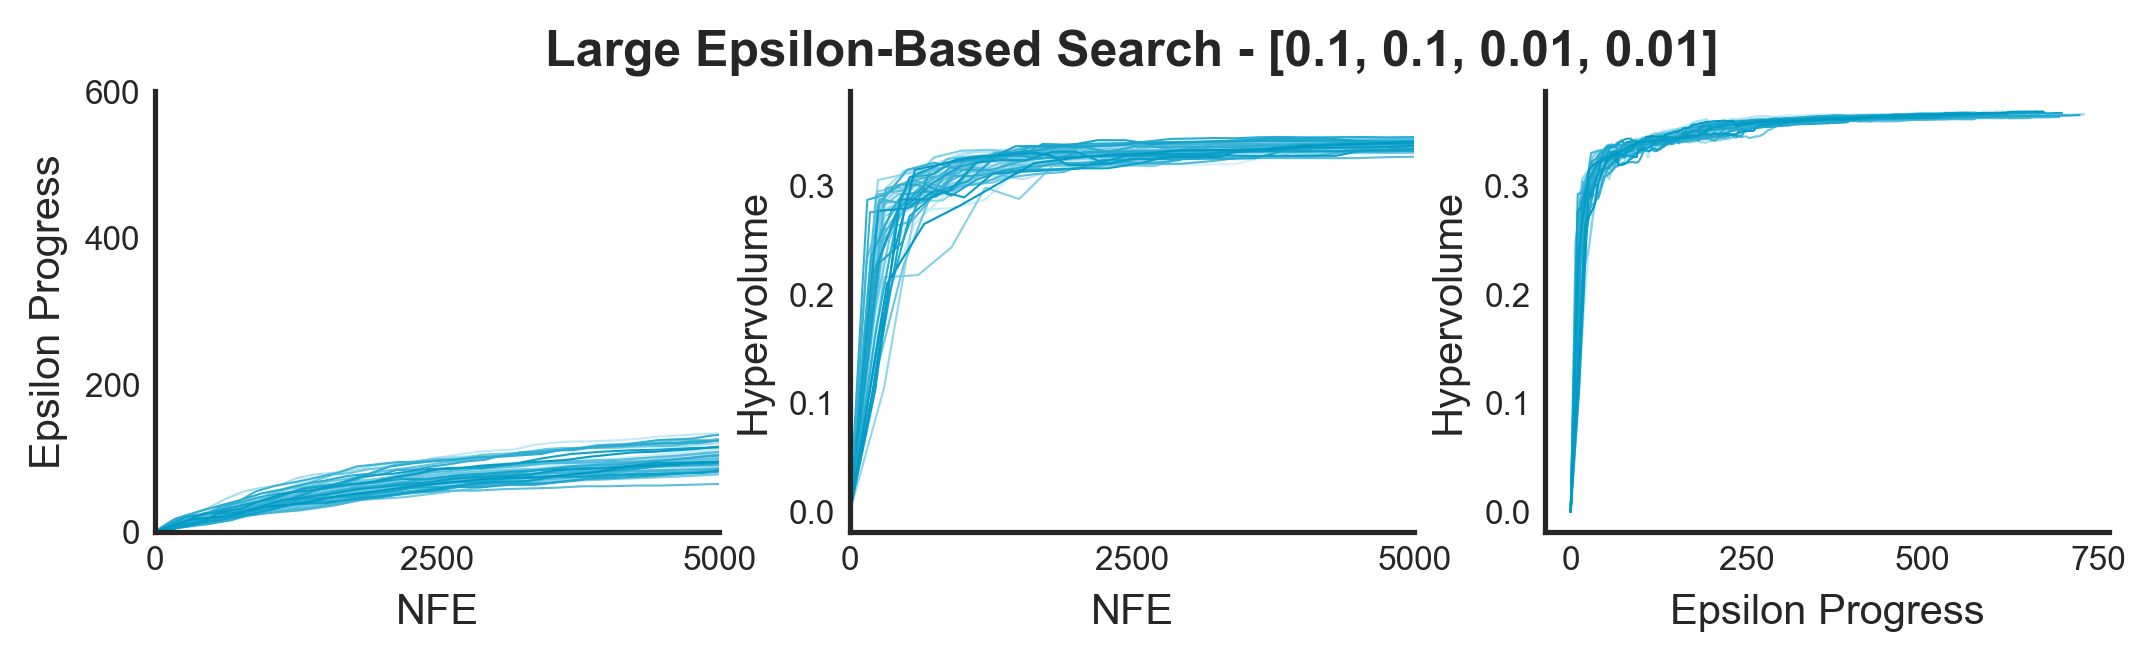
\includegraphics[width=\textwidth]{appendices/epsilon_settings/bigeps_convergence_dps_highres}
        \label{fig:appendix-bigeps}
    \end{subfigure}
    \begin{subfigure}[b]{\textwidth}
        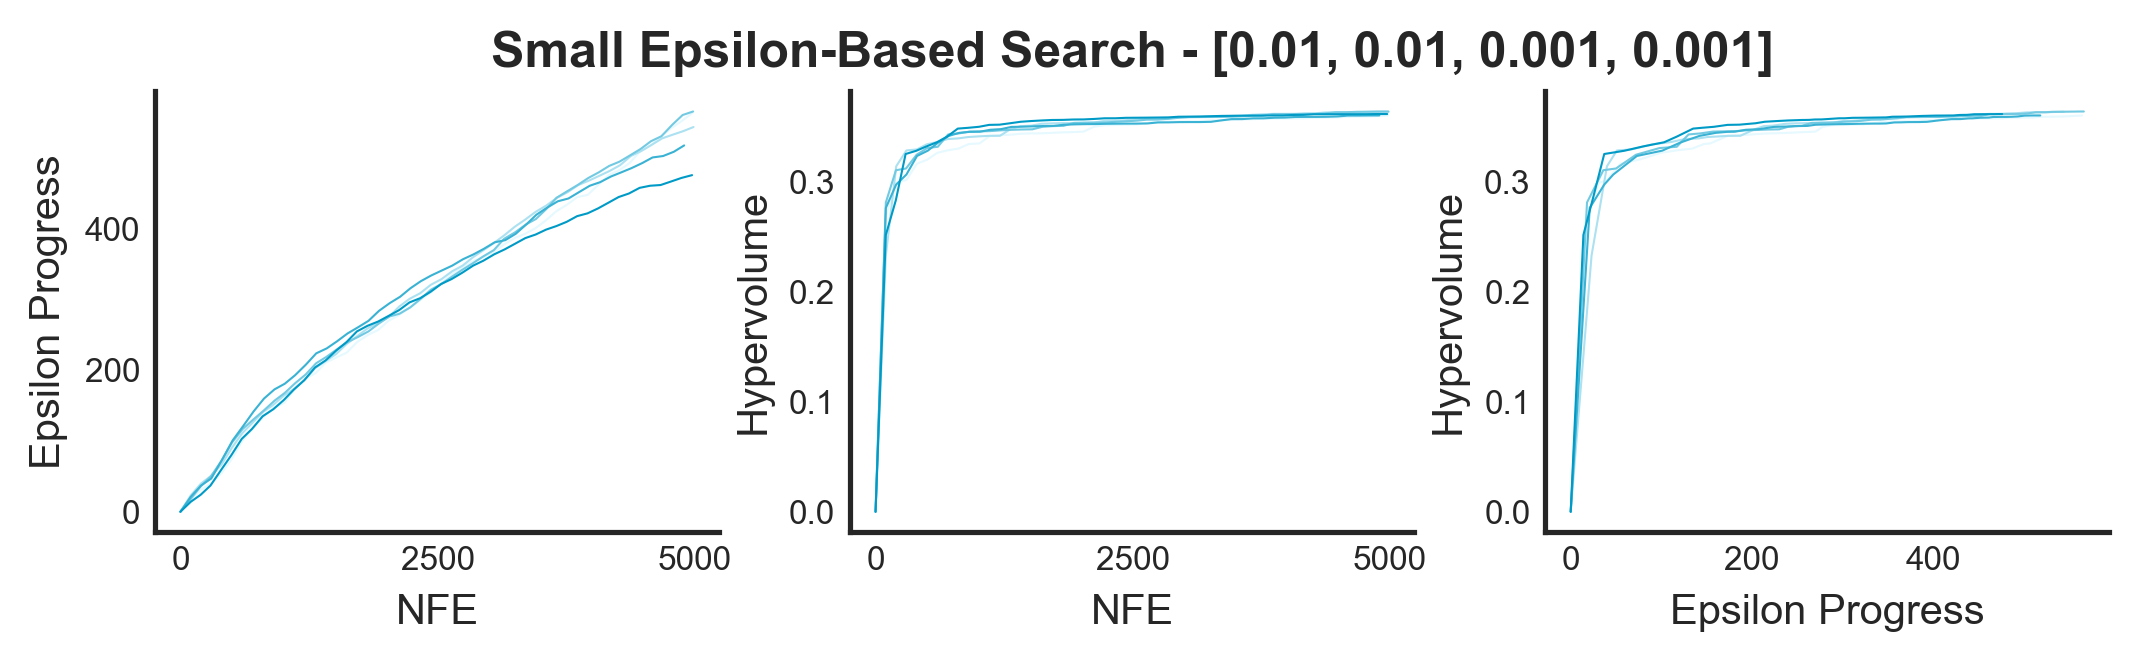
\includegraphics[width=\textwidth]{appendices/epsilon_settings/smalleps_convergence_dps_highres}
        \label{fig:appendix-smalleps}
    \end{subfigure}
    
    \caption[Comparing convergence with different epsilon value settings]{Comparison of the convergence of two MOEA-based searches of the DPS model variation and MORDM pairing using two different epsilon value settings, where the order follows [pollution level, utility, inertia, reliability]. }
    \label{fig:appendix-epsiloncompare}
\end{figure}

\cref{fig:appendix-epsiloncompare} shows the convergence plots for the two sets of epsilon values being compared here. For the sake of the comparison, the number of function executions visible in the case of the large epsilon-based search was limited to 5000, matching the number of function executions used for the small epsilon value. The epsilon progress numbers are quite different between the two settings, with the small epsilon values yielding a much larger epsilon progress value by function execution 5000. This is consistent with the size of epsilon values used in the two sets of charts. As epsilon progress tracks search progress based on the number of policies added to the non-dominated set of alternatives, and because a set of smaller epsilon values will yield a larger number of policies in that set, the epsilon progress should and does increase at a faster rate. 

Hypervolume convergence in \cref{fig:appendix-epsiloncompare}, however, is quite similar between the two settings, both in shape and in value. This indicates that despite significantly different epsilon progress, the sets of non-dominated policy alternatives are covering a similar volume of space within the space described by the set of decision levers and defined in \cref{table:moeaadditional}. 

\begin{table}[h]
    \centering
    \captionsetup{width=0.7\textwidth}
    \caption{Sizes of the non-dominated Pareto front for both small and large epsilon value settings.}
    \label{table:appendix-epsilon-paretosize}
    
    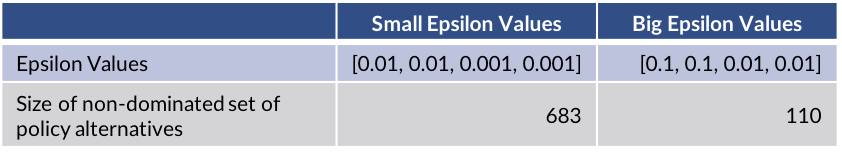
\includegraphics[width=0.7\textwidth]{appendices/epsilon_settings/sizeoffront}
\end{table}

\begin{figure}[h]
    \centering
    \captionsetup{width=\textwidth}
    
    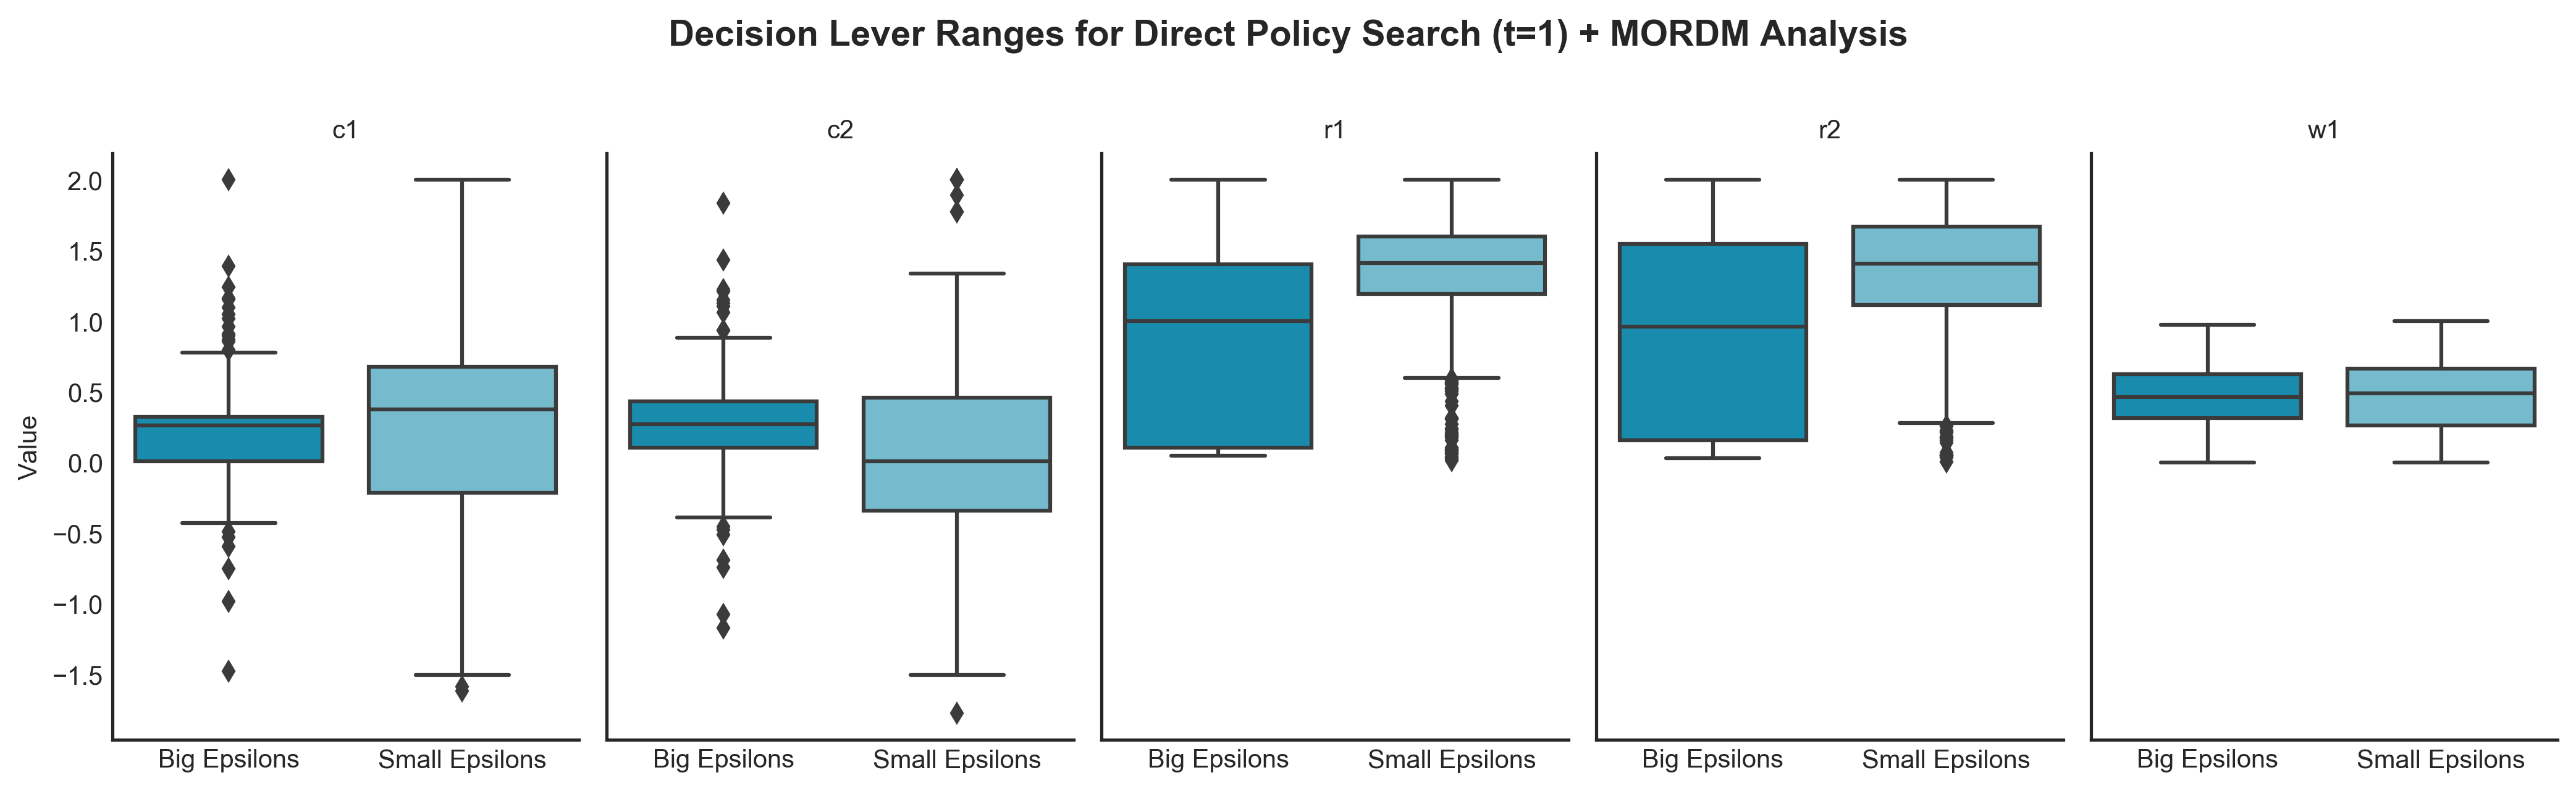
\includegraphics[width=\textwidth]{appendices/epsilon_settings/leverranges_epsilons_box_highres}
    
    \caption[Comparing decision lever values with different epsilon value settings]{Comparison of the ranges of decision lever values between changing epsilon values in the search phase.}
    \label{fig:appendix-epsilondecisionlevers}
\end{figure}

\begin{figure}[h]
    \centering
    \captionsetup{width=0.5\textwidth}
    
    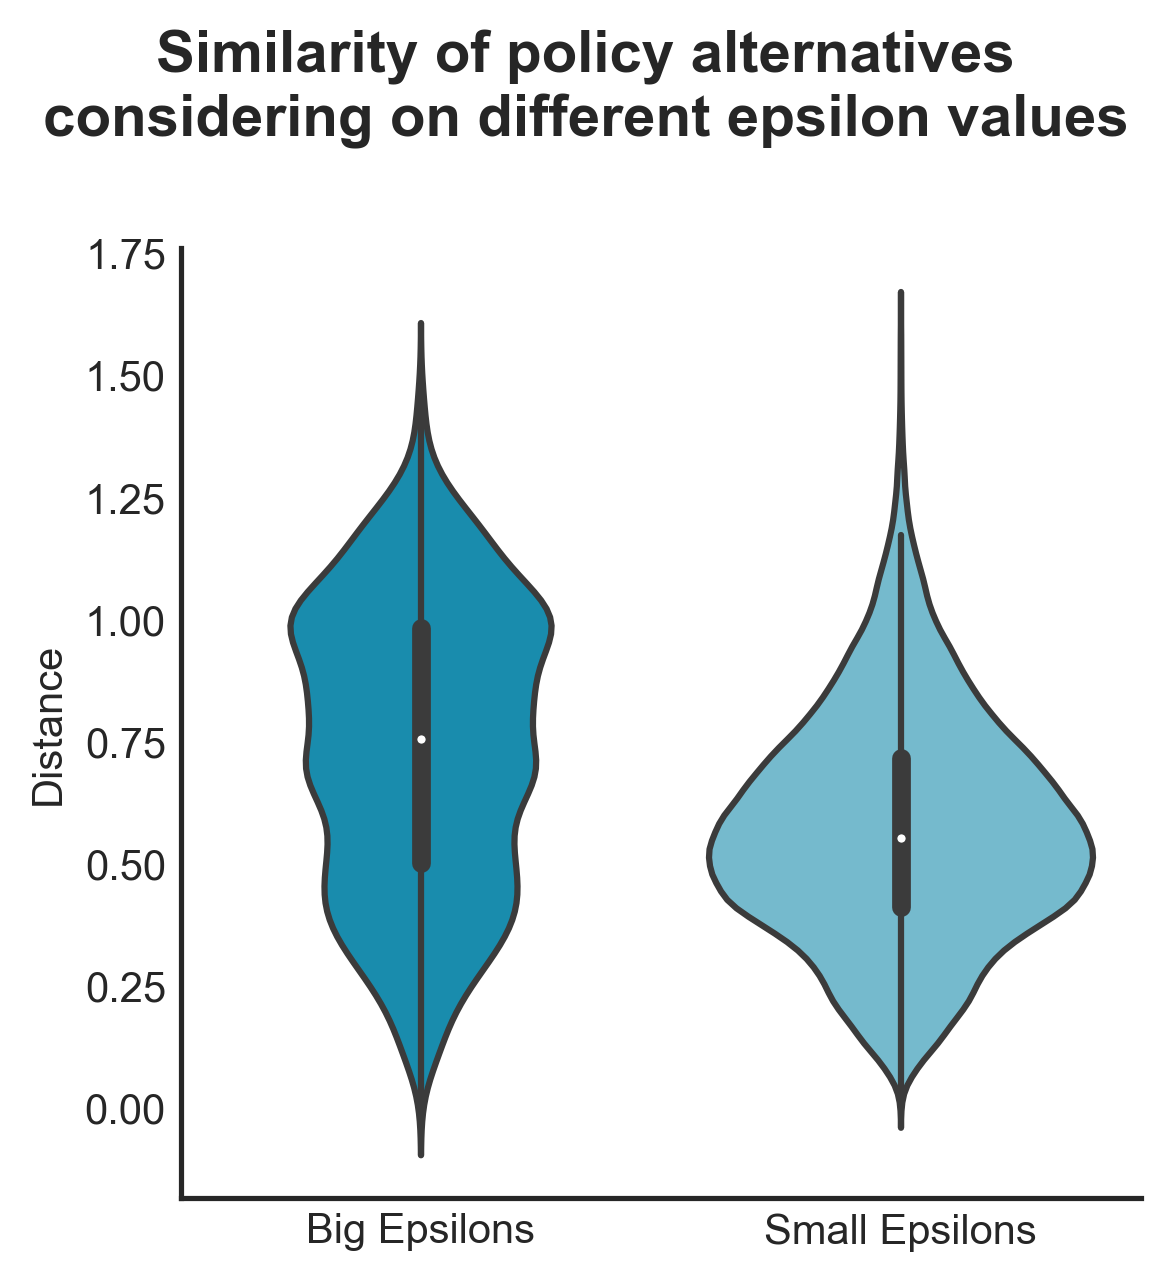
\includegraphics[width=0.3\textwidth]{appendices/epsilon_settings/epsilons_similarity_violin_highres}
    
    \caption[Comparing similarity of alternatives with different epsilon value settings]{Comparison of the similarity of non-dominated policy alternatives for different epsilon settings.}
    \label{fig:appendix-epsilonsimilarity}
\end{figure}

As mentioned earlier, a set of smaller epsilon values will lead to a larger set of non-dominated alternatives, because polices will be included in the set that are closer in value than would be with a set of larger epsilon values. This is borne out in \cref{table:appendix-epsilon-paretosize}, which shows the size of the non-dominated set of policy alternatives for both epsilon value settings. In this case, the number of policy alternatives is over six times larger with smaller epsilon values than seen in this study, which has made use of the larger values. 

The final comparison done is found in \cref{fig:appendix-epsilondecisionlevers}, and \cref{fig:appendix-epsilonsimilarity} which compares the ranges of values for each decision lever of the DPS model variation. Depending on the decision lever, both the larger and smaller epsilon values produce a set of polices with a wider range of values. This indicates that using smaller epsilon values will not necessarily lead to greater diversity of policy alternatives in the case of the lake problem. In fact, \cref{fig:appendix-epsilonsimilarity} seems to confirm that despite the significantly larger size of the non-dominated set of alternatives obtained with smaller epsilon values, the larger epsilon values produce a more diverse set of policy alternatives. It is possible that due to the significantly smaller number of function executions performed with the smaller epsilon values, that the diversity of the set of non-dominated alternatives would have been larger, but these results confirm, at least, that the larger epsilon values are able to produce a set of alternatives with a similar hypervolume and greater diversity than smaller epsilon values would have. Therefore, selecting larger epsilon values should have no negative impact to the results of this study. 

%TODO Also can show robustness changes. EEB


 %DONE for now
\chapter{MOEA Operator Convergence}
\label{appendix-operatorconvergence}

In addition to overall epsilon progress and hypervolume convergence, the likelihood of each operator being selected for a generation was tracked throughout the search process. The likelihood of selection is updated after each generation based on how successful that operator was at identifying non-dominated policy alternatives. To contrast with the five operators available to the auto-adaptive $\epsilon$-NSGAII algorithm, traditional $\epsilon$-NSGAII uses a single operator: simulated binary crossover (SBX) variator + polynomial mutation (PM) mutator \citep{Reed2013}.

\section{Intertemporal}
Each of the analyses using the intertemporal model, shown in \cref{fig:operatorconvergence-inter} quickly converge to using a uniform mutation (UM) almost 100 percent of the time. This indicates that the best operator for convergence with respect to the intertemporal problem is not the SBX operator used by traditional $\epsilon$-NSGAII, but another operator entirely. This result matches the failure of several MOEAs, including $\epsilon$-NSGAII, to find a strong set of policy alternatives \citep{Ward2015}. This same study also found Borg to be the only successful MOEA of the ones tested with respect to the intertemporal problem variation. Given the search success found in this study, the proposed auto-adaptive $\epsilon$-NSGAII algorithm remains a promising alternative to Borg. The SBX and parent-centric crossover (PCX) operators maintain some likelihood of use for a subset of the search repetitions. However, the maximum likelihood for both after the initial startup does not reach higher than the original likelihood of use of 15 percent, so use of those operators continued to be uncommon. 

\section{Planned adaptive DPS}
The planned adaptive DPS operator selection, shown in \cref{fig:operatorconvergence-planned} did not converge to a single operator like the intertemporal analyses did. The most commonly used operators in each of the intertemporal analyses are the PCX, SBX, and UM. There is wide variation between each repetition of the search process as to which operator is more likely to be selected, however.

\section{Direct Policy Search}
The DPS-based analyses and corresponding operator selection convergences are shown in \cref{fig:operatorconvergence-dps}. The multi-scenario MORDM and MORO analyses display similar behavior as with the planned adaptive DPS model variation. There is some interesting behavior in the MORDM analysis, however. As \cref{fig:convergences-dps} showed, the epsilon progress trend reaches a steady level initially and then begins to increase again at around 50,000 function executions, leveling out as progress reaches 100,000 function executions. Correspondingly with that behavior are the likelihood trends of both the UM and SBX operators. Initially, The UM operator is significantly more likely to be selected than the SBX operator. Then, at around 50,000 function executions, there is a transition between the two operators, and the SBX operator becomes more likely to be selected than the UM operator. This information indicates that the auto-adaptive $\epsilon$-NSGAII algorithm realized that it was no longer able to make progress with the UM operator, but that the SBX operator was still discovering new non-dominated policy alternatives, and was able to transition between the two operators to continue progressing in the search. However, referring to the hypervolume convergence in \cref{fig:convergences-dps}, the epsilon-based progress made using the SBX operator did not result in alternatives that contributed to an increase in hypervolume of the non-dominated set. 

\begin{figure}[ht]
    \centering
    \captionsetup{width=0.85\textwidth}
    
    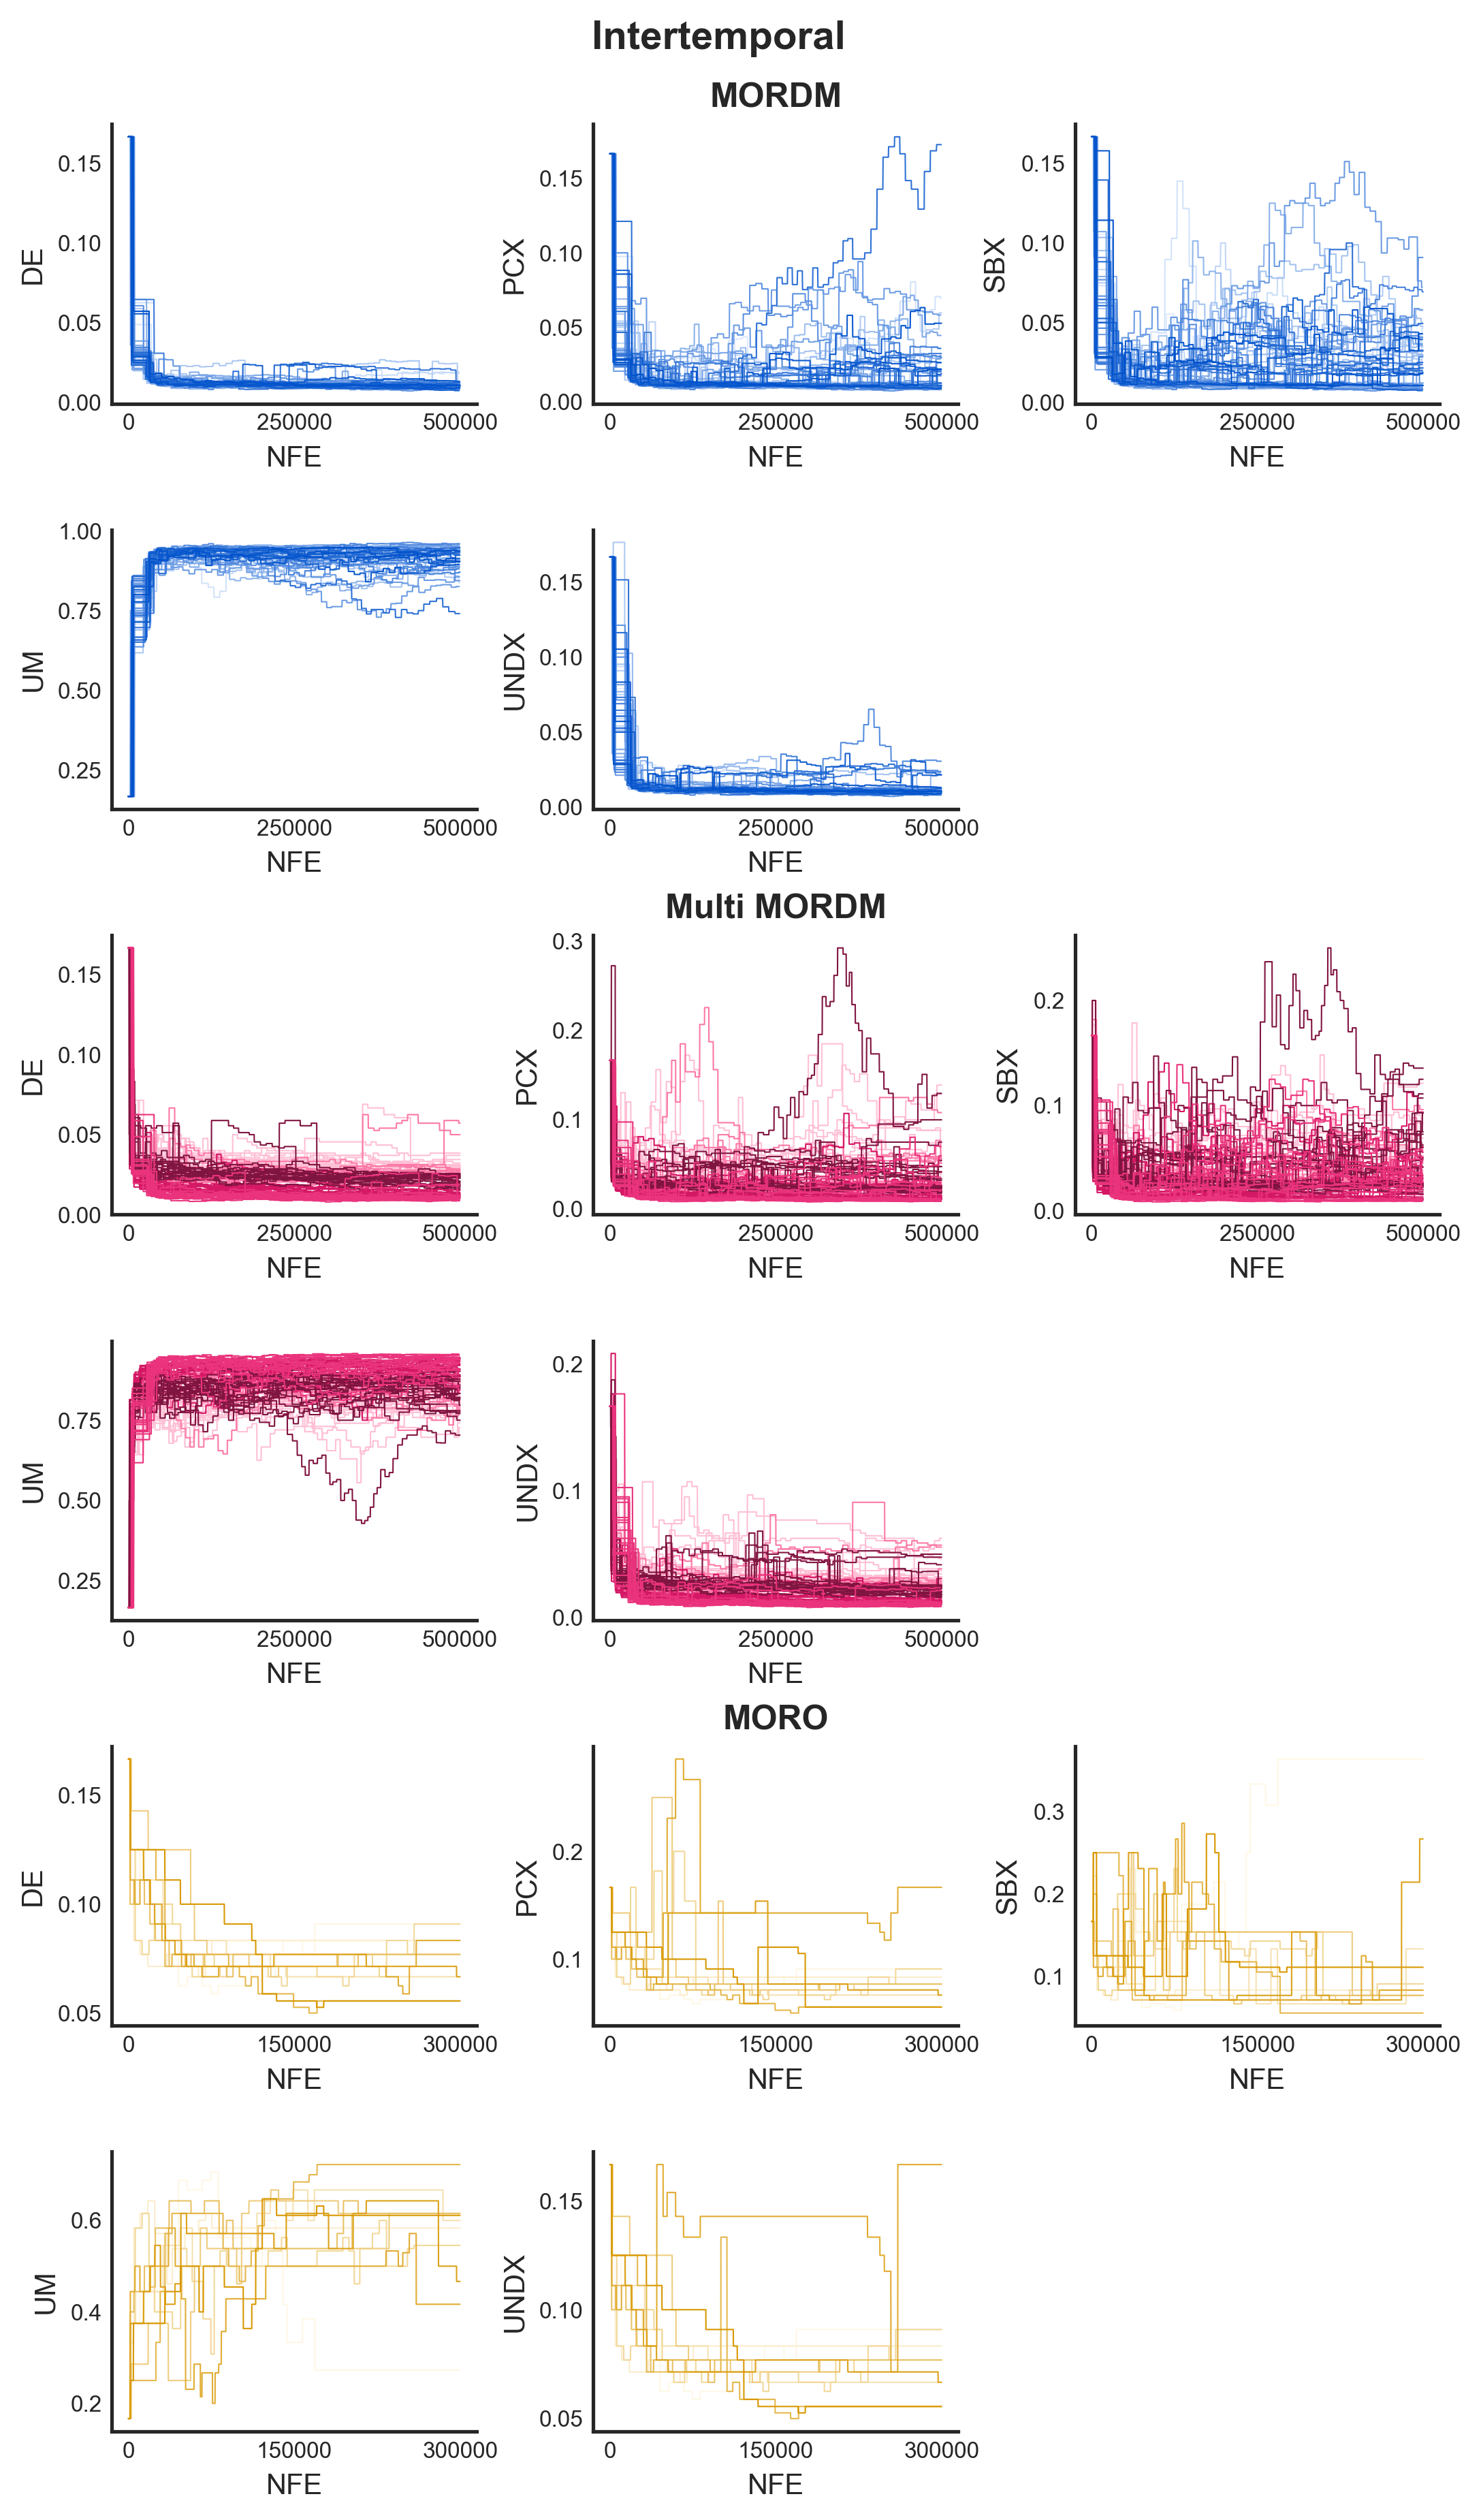
\includegraphics[width=0.85\textwidth]{appendices/operator_convergence/operatorconvergence_inter}
    \caption[Operator convergence for the intertemporal model variation]{The convergence of the five operators used in the Auto-Adaptive $\epsilon$-NSGAII operator selection for all methods using the intertemporal lake model variation.}
    \label{fig:operatorconvergence-inter}
\end{figure}

\begin{figure}[ht]
    \centering
    \captionsetup{width=0.85\textwidth}
    
    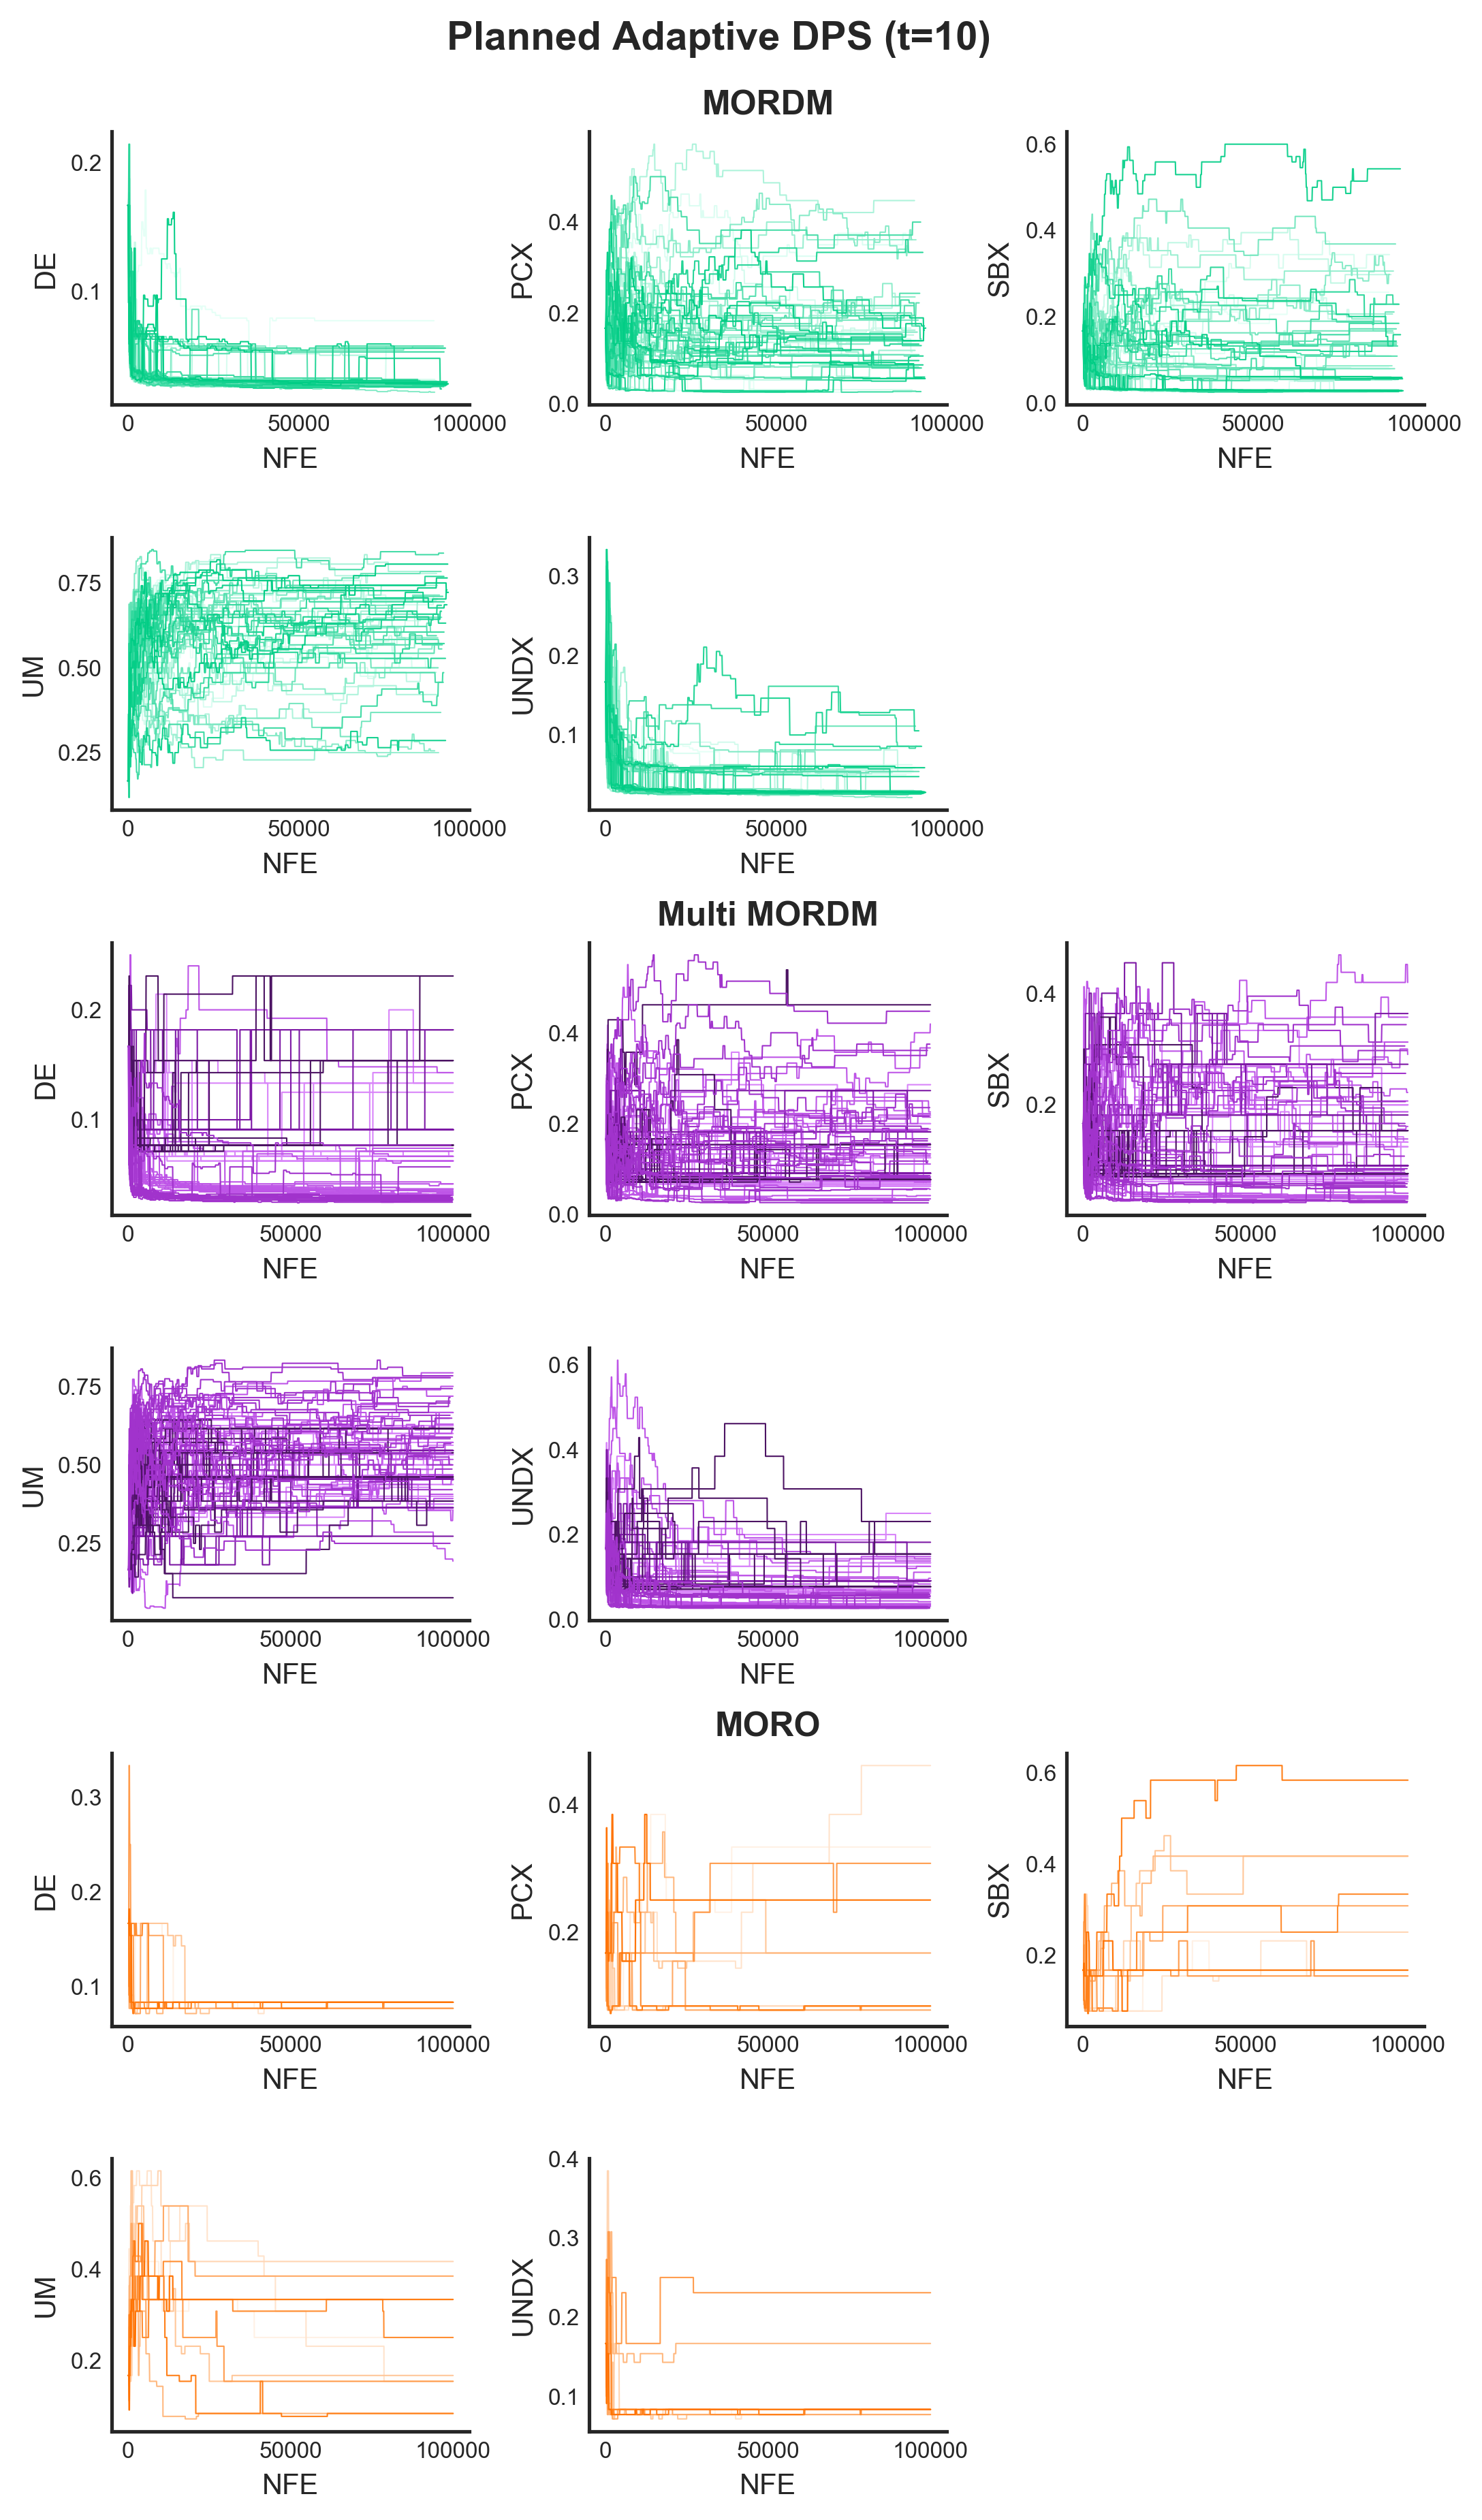
\includegraphics[width=0.85\textwidth]{appendices/operator_convergence/operatorconvergence_planned}
    \caption[Operator convergence for the planned adaptive DPS model variation]{The convergence of the five operators used in the Auto-Adaptive $\epsilon$-NSGAII operator selection for all methods using the planned adaptive DPS lake model variation.}
    \label{fig:operatorconvergence-planned}
\end{figure}

\begin{figure}[ht]
    \centering
    \captionsetup{width=0.85\textwidth}
    
    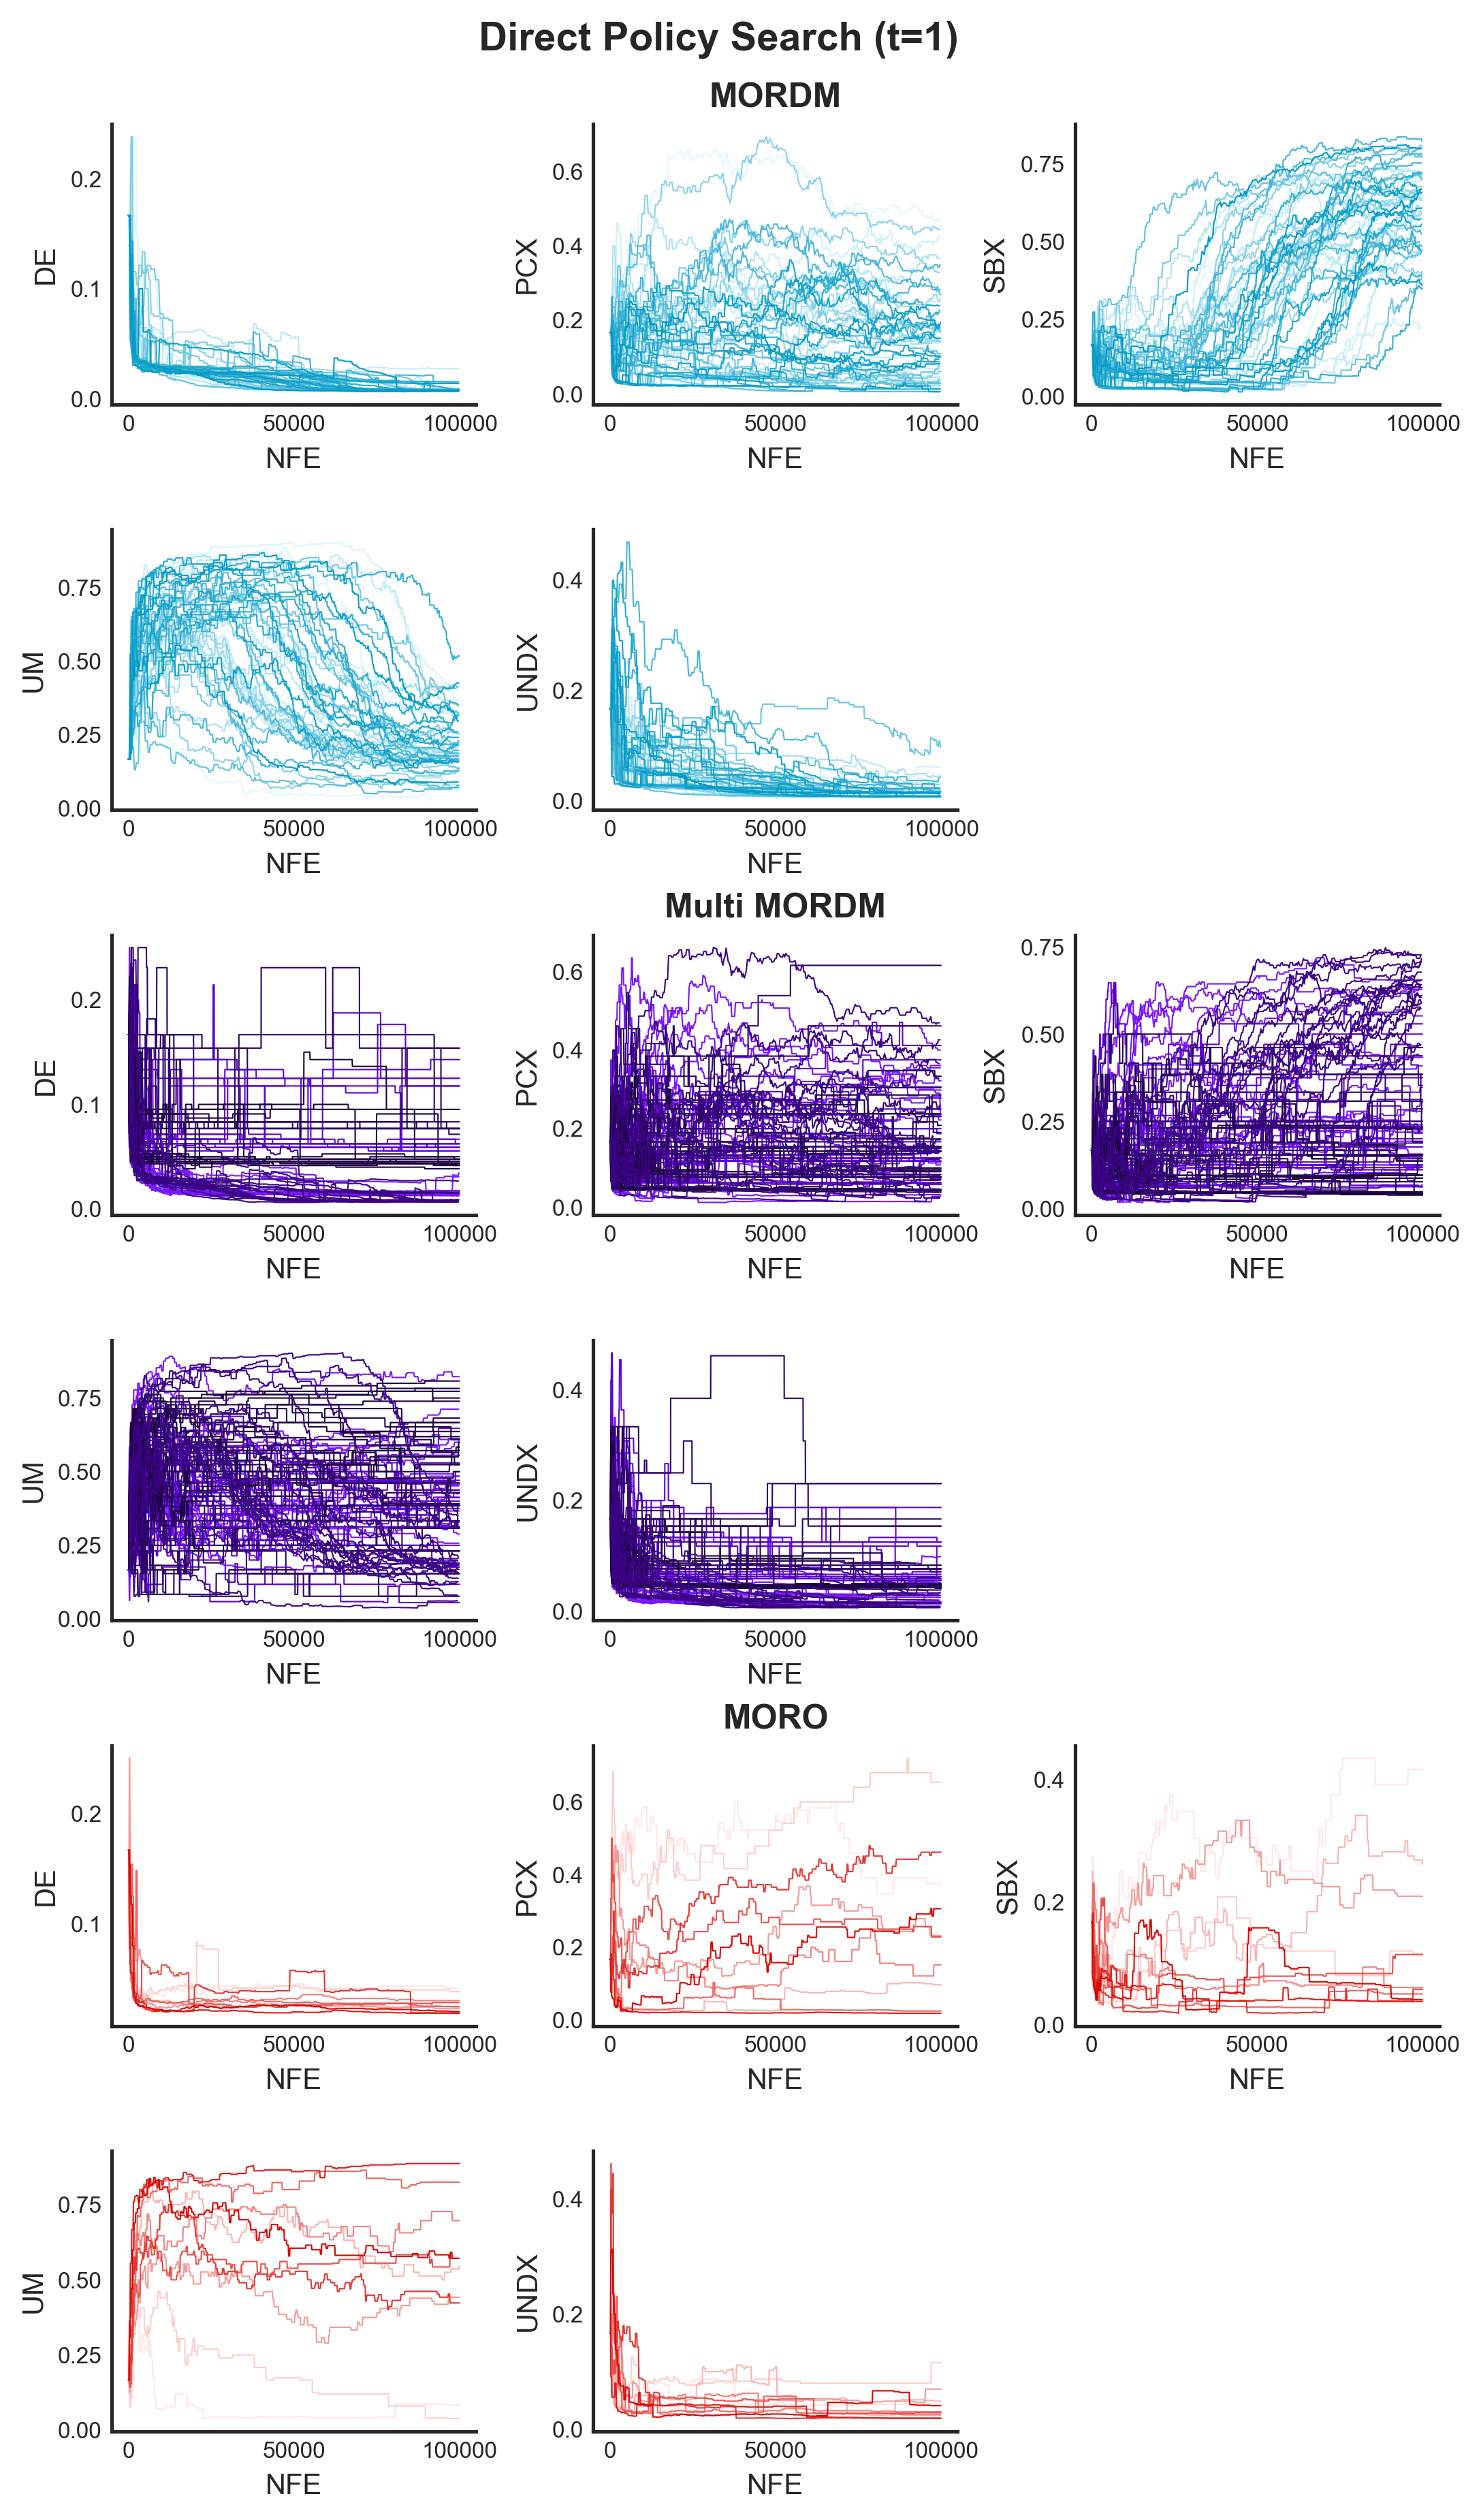
\includegraphics[width=0.85\textwidth]{appendices/operator_convergence/operatorconvergence_dps}
    \caption[Operator convergence for the DPS model variation]{The convergence of the five operators used in the Auto-Adaptive $\epsilon$-NSGAII operator selection for all methods using the DPS lake model variation.}
    \label{fig:operatorconvergence-dps}
\end{figure} %DONE
\chapter{MOEA Random Seed Analysis}
\label{appendix-seedanalysis}

This appendix considers the impact of the random seed to the results of the MOEA-based search process for each method. The random seed influences the initial population selection for each repetition, which uses Latin Hypercube Sampling, among other functionality. Analysis is broken down per robust decision support method. 

\section{MORDM} \label{seedanalysis-mordm}
The results of the random seed analysis for each MORDM-based analysis is shown in \cref{fig:pareto-mordm} and includes three types of plots. The first column displays the size of the identified non-dominated Pareto front size for each search repetition. The second column shows hypervolume of the final non- dominated policy set. The final column compares the size of the non-dominated set of policy alternatives to the hypervolume of each set. 

\begin{figure}[H]
    \centering
    
    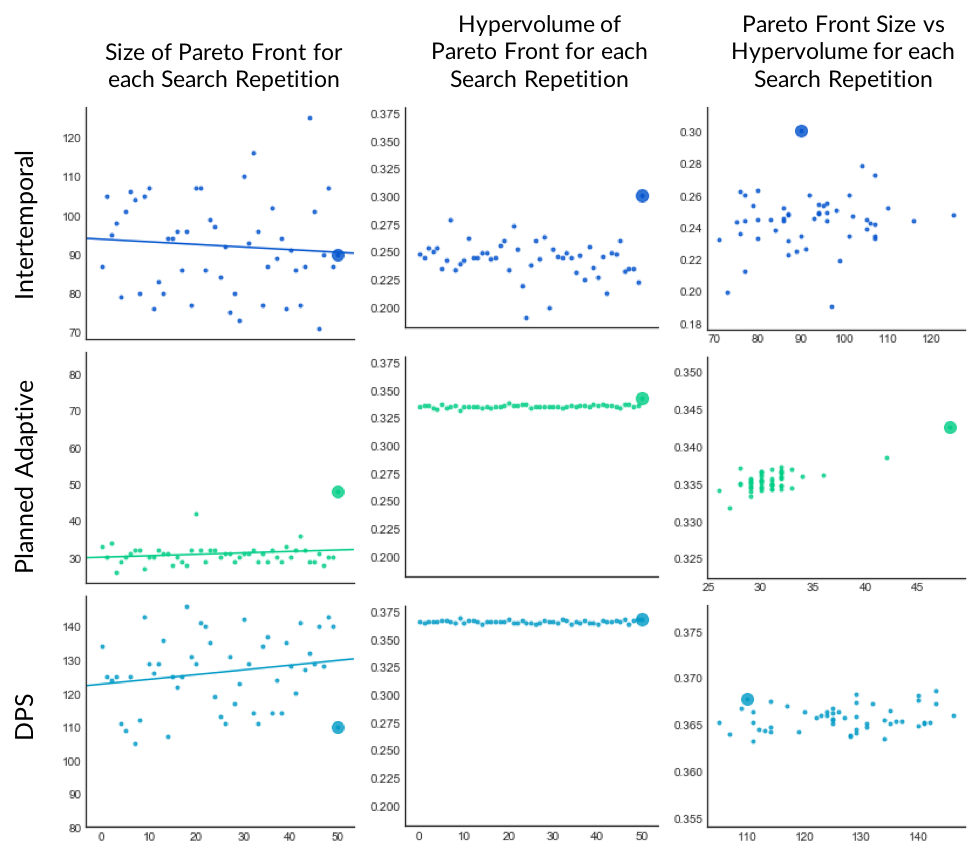
\includegraphics[width=0.75\textwidth]{appendices/seed_analysis/paretosize_mordm}
    \caption[Random seed analysis for all uses of MORDM]{Random seed analysis for the MORDM robust decision support method. The large circle represents the set of non-dominated alternatives that combines the results from each search repetition.}
    \label{fig:pareto-mordm}
\end{figure}

The final combined non-dominated set of policy alternatives for the intertemporal analysis yields a number of policy alternatives that is similar to the results found in each search repetition. However, as indicated by the plot in the second column, that final combined set does result in a larger hypervolume than a single search repetition. This indicates that using multiple search repetitions did improve the diversity of the final policy set without increasing the size of the set, providing a stronger foundation for the future steps in the analysis. 

In contrast, despite the combined non-dominated set of alternatives containing a larger number of policies, the hypervolume was not increased with respect to the planned adaptive DPS model variation. In fact, the hypervolume of each search repetition is extremely constant, indicating that the random seed does not have any real impact on the diversity of the final non-dominated set of policy alternatives. 

Finally, the combined results for the DPS model variation include a smaller number of policy alternatives than most of the stand-alone search repetitions. At the same time, that front is able to maintain a similar hypervolume as each stand-alone repetition. This indicates that considering multiple repetitions of an MOEA-based search leads to a smaller set of non-dominated alternatives that are just as diverse as an individual repetition. Such a smaller set may prove easier for decision makers to manage in the later steps of an analysis. 

\section{Multi-Scenario MORDM}

\begin{figure}[H]
    \centering
    
    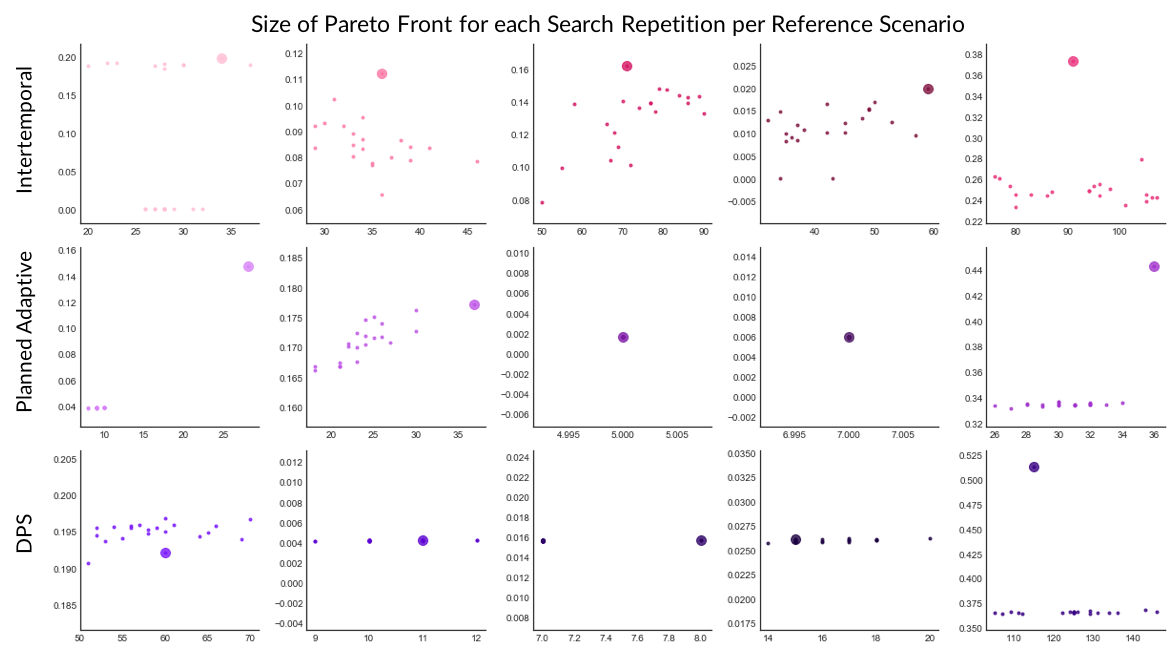
\includegraphics[width=0.95\textwidth]{appendices/seed_analysis/paretosize_multi_front}
    \caption[Pareto front size across search repetitions for multi-scenario MORDM]{Size of the pareto front for each search repetition of all multi-scenario MORDM analyses.}
    \label{fig:pareto-multi-size}
\end{figure}

\begin{figure}[H]
    \centering
    
    \includegraphics[width=0.95\textwidth]{appendices/seed_analysis/paretosize_multi_hypervolume}
    \caption{Hypervolume of the pareto front for all multi-scenario MORDM analyses.}
    \label{fig:pareto-multi-volume}
\end{figure}

\begin{figure}[H]
    \centering
    
    \includegraphics[width=0.95\textwidth]{appendices/seed_analysis/paretosize_multi_vs}
    \caption{The relationship between hypervolume and pareto front size across all multi-scenario MORDM analyses.}
    \label{fig:pareto-multi-versus}
\end{figure}

\begin{figure}[H]
    \centering
    
    \includegraphics[width=0.75\textwidth]{appendices/seed_analysis/paretosize_moro}
    \caption[Random seed analysis for all uses of MORO]{Random seed analysis for the MORO robust decision support method. The large circle represents the set of non-dominated alternatives that combines the results from each search repetition.}
    \label{fig:pareto-moro}
\end{figure}

\section{MORO}
The results of the random seed analysis for each MORO-based analysis is shown in \cref{fig:pareto-moro} and  includes three types of plots. The first column displays the size of the identified non-dominated Pareto front size for each search repetition. The second column shows hypervolume of the final set of policy alternatives. The final column compares the size of the non-dominated set of policy alternatives to the hypervolume of each set. 

The results of the random seed analysis for each of the lake problem variations is similar to what is identified in the MORDM-based seed analysis, despite the average size of the set of non-dominated policy alternatives being considerably smaller. With respect to the intertemporal analysis, a somewhat higher diversity is achieved with a smaller set of alternatives in the combined non-dominated set. The planned adaptive DPS analysis leads to a higher diversity of policy alternatives despite maintaining a similar size in the combined set of non-dominated policy alternatives. And finally, the DPS results lead to a somewhat higher hypervolume and a combined non-dominated set size that is among the smallest obtained across all search repetitions. 
 
\chapter{Results of Uncertainty Analysis}
\label{appendix-uncertainty}

A summary of the results of each model variation and method pairing was included in the main text of this study. This appendix will include a more detailed look at the individual results of the uncertainty analysis, for reference. To accomplish this, the data gathered will be visualized as pair plots, which visualize the relationships between each pair of outcome variables. These plots can reveal relationships between outcomes of interest that are useful in analysis and decision making. 

\section{Intertemporal Results}

\begin{figure}[h]
    \centering
    
    \includegraphics[width=\textwidth]{appendices/uncertainty_analysis/mordm_intertemporal}
    \caption[Intertemporal + MORDM pair plot]{Pair-plot showing the results of uncertainty analysis for a MORDM-based analysis of the intertemporal lake problem.}
    \label{fig:pairplot-mordm-inter}
\end{figure}

Very few relationships of any significance are revealed in \cref{fig:pairplot-mordm-inter}, graphing the results of the intertemporal and MORDM pairing. The plot does show a negative correlation between pollution level and reliability. Given that reliability refers to the ability of the policy to maintain low levels of pollution, it follows quite easily that higher pollution levels is paired with lower policy reliability. That same relationship is seen in \cref{fig:pairplot-multi-inter}, the plot of the results of the intertemporal and multi-scenairo MORDM pairing and even more significantly in \cref{fig:pairplot-moro-inter}, the results of the intertemporal and MORO pairing. 

\begin{figure}[h!]
    \centering
    
    \includegraphics[width=\textwidth]{appendices/uncertainty_analysis/multi_intertemporal}
    \caption[Intertemporal + multi-scenario MORDM pair plot]{Pair-plot showing the results of uncertainty analysis for a multi-scenario MORDM-based analysis of the intertemporal lake problem.}
    \label{fig:pairplot-multi-inter}
\end{figure}

\cref{fig:pairplot-moro-inter}, the results of the intertemporal and MORO pairing, also reveal interesting behavior with respect to the inertia of identified policies, where only very low and very high values for inertia are reported. This behavior was investigated in more detail in \cref{chapter-comparison}. 

\begin{figure}[H]
    \centering
    
    \includegraphics[width=\textwidth]{appendices/uncertainty_analysis/moro_intertemporal}
    \caption[Intertemporal + MORO pair plot]{Pair-plot showing the results of uncertainty analysis for a MORO-based analysis of the intertemporal lake problem.}
    \label{fig:pairplot-moro-inter}
\end{figure}

\newpage

\section{Planned Adaptive DPS Results} \label{pairplots-planned}
The relationship between pollution and reliability continues across all methods in the case of the planned adaptive DPS variation, though that relationship does not appear as strong in the multi-scenario MORDM case as it is for the other two methods. Both the multi-scenario MORDM and MORO methods seem to report a slight positive relationship between inertia and pollution level, where higher pollution levels lead to higher policy inertia. Given that policy inertia indicates that the amount of pollution released in each time step does not change significantly, it is not surprising that more constant rates of release may lead to higher levels of pollution in the lake. Interestingly, the opposite relationship is seen in the MORDM analysis of the planned adaptive DPS model, where higher levels of inertia lead to lower pollution levels. It is unclear given these pair plots why the relationship between the two outcomes of interest is different in the MORDM case than with the other two methods. 

\begin{figure}[H]
    \centering
    
    \includegraphics[width=\textwidth]{appendices/uncertainty_analysis/mordm_planned}
    \caption[Planned adaptive DPS + MORDM pair plot]{Pair-plot showing the results of uncertainty analysis for a MORDM-based analysis of the planned adaptive DPS lake problem.}
    \label{fig:pairplot-mordm-planned}
\end{figure}

\begin{figure}[H]
    \centering
    
    \includegraphics[width=\textwidth]{appendices/uncertainty_analysis/multi_planned}
    \caption[Planned adaptive DPS + multi-scenario MORDM pair plot]{Pair-plot showing the results of uncertainty analysis for a multi-scenario MORDM-based analysis of the planned adaptive DPS lake problem.}
    \label{fig:pairplot-multi-planned}
\end{figure}

\begin{figure}[H]
    \centering
    
    \includegraphics[width=\textwidth]{appendices/uncertainty_analysis/moro_planned}
    \caption[Planned adaptive DPS + MORO pair plot]{Pair-plot showing the results of uncertainty analysis for a MORO-based analysis of the planned adaptive DPS lake problem.}
    \label{fig:pairplot-moro-planned}
\end{figure}

\newpage

\section{Direct Policy Search Results}

The final set of pair plots involve the DPS model variation. The negative relationship between pollution level and reliability is not as strong for all three methods using the DPS model variation, as compared to the other two variations. There exists, however, a strong positive correlation between pollution and inertia for all three methods similar to what is seen and discussed in \cref{pairplots-planned}. An even stronger negative relationship between inertia and reliability is seen across all three methods as well, where higher levels of inertia lead to lower reliability. This relationship matches the relationships between pollution and reliability, and between inertia and reliability described previously. Higher levels of inertia mean the pollution level is not updated as frequently, which can make it more likely for the pollution level in the lake to rise and therefore reliability of that policy to decline.

\begin{figure}[H]
    \centering
    
    \includegraphics[width=\textwidth]{appendices/uncertainty_analysis/mordm_dps}
    \caption[DPS + MORDM pair plot]{Pair-plot showing the results of uncertainty analysis for a MORDM-based analysis of the DPS lake problem.}
    \label{fig:pairplot-mordm-dps}
\end{figure}

\begin{figure}[H]
    \centering
    
    \includegraphics[width=\textwidth]{appendices/uncertainty_analysis/multi_dps}
    \caption[DPS + multi-scenario MORDM pair plot]{Pair-plot showing the results of uncertainty analysis for a multi-scenario MORDM-based analysis of the DPS lake problem.}
    \label{fig:pairplot-multi-dps}
\end{figure}

\begin{figure}[H]
    \centering
    
    \includegraphics[width=\textwidth]{appendices/uncertainty_analysis/moro_dps}
    \caption[DPS + MORO pair plot]{Pair-plot showing the results of uncertainty analysis for a MORO-based analysis of the DPS lake problem.}
    \label{fig:pairplot-moro-dps}
\end{figure} %DONE

%% Turn off thumb indices for unnumbered chapters.
\thumbfalse

\end{document}
